% Options for packages loaded elsewhere
\PassOptionsToPackage{unicode}{hyperref}
\PassOptionsToPackage{hyphens}{url}
%
\documentclass[
  letterpaper,
  10pt,
  reqno,
  twopage,
  openany]{book}

\usepackage{amsmath,amssymb}
\usepackage{lmodern}
\usepackage{iftex}
\ifPDFTeX
  \usepackage[T1]{fontenc}
  \usepackage[utf8]{inputenc}
  \usepackage{textcomp} % provide euro and other symbols
\else % if luatex or xetex
  \usepackage{unicode-math}
  \defaultfontfeatures{Scale=MatchLowercase}
  \defaultfontfeatures[\rmfamily]{Ligatures=TeX,Scale=1}
\fi
% Use upquote if available, for straight quotes in verbatim environments
\IfFileExists{upquote.sty}{\usepackage{upquote}}{}
\IfFileExists{microtype.sty}{% use microtype if available
  \usepackage[]{microtype}
  \UseMicrotypeSet[protrusion]{basicmath} % disable protrusion for tt fonts
}{}
\makeatletter
\@ifundefined{KOMAClassName}{% if non-KOMA class
  \IfFileExists{parskip.sty}{%
    \usepackage{parskip}
  }{% else
    \setlength{\parindent}{0pt}
    \setlength{\parskip}{6pt plus 2pt minus 1pt}}
}{% if KOMA class
  \KOMAoptions{parskip=half}}
\makeatother
\usepackage{xcolor}
\setlength{\emergencystretch}{3em} % prevent overfull lines
\setcounter{secnumdepth}{5}
% Make \paragraph and \subparagraph free-standing
\ifx\paragraph\undefined\else
  \let\oldparagraph\paragraph
  \renewcommand{\paragraph}[1]{\oldparagraph{#1}\mbox{}}
\fi
\ifx\subparagraph\undefined\else
  \let\oldsubparagraph\subparagraph
  \renewcommand{\subparagraph}[1]{\oldsubparagraph{#1}\mbox{}}
\fi


\providecommand{\tightlist}{%
  \setlength{\itemsep}{0pt}\setlength{\parskip}{0pt}}\usepackage{longtable,booktabs,array}
\usepackage{calc} % for calculating minipage widths
% Correct order of tables after \paragraph or \subparagraph
\usepackage{etoolbox}
\makeatletter
\patchcmd\longtable{\par}{\if@noskipsec\mbox{}\fi\par}{}{}
\makeatother
% Allow footnotes in longtable head/foot
\IfFileExists{footnotehyper.sty}{\usepackage{footnotehyper}}{\usepackage{footnote}}
\makesavenoteenv{longtable}
\usepackage{graphicx}
\makeatletter
\def\maxwidth{\ifdim\Gin@nat@width>\linewidth\linewidth\else\Gin@nat@width\fi}
\def\maxheight{\ifdim\Gin@nat@height>\textheight\textheight\else\Gin@nat@height\fi}
\makeatother
% Scale images if necessary, so that they will not overflow the page
% margins by default, and it is still possible to overwrite the defaults
% using explicit options in \includegraphics[width, height, ...]{}
\setkeys{Gin}{width=\maxwidth,height=\maxheight,keepaspectratio}
% Set default figure placement to htbp
\makeatletter
\def\fps@figure{htbp}
\makeatother
\newlength{\cslhangindent}
\setlength{\cslhangindent}{1.5em}
\newlength{\csllabelwidth}
\setlength{\csllabelwidth}{3em}
\newlength{\cslentryspacingunit} % times entry-spacing
\setlength{\cslentryspacingunit}{\parskip}
\newenvironment{CSLReferences}[2] % #1 hanging-ident, #2 entry spacing
 {% don't indent paragraphs
  \setlength{\parindent}{0pt}
  % turn on hanging indent if param 1 is 1
  \ifodd #1
  \let\oldpar\par
  \def\par{\hangindent=\cslhangindent\oldpar}
  \fi
  % set entry spacing
  \setlength{\parskip}{#2\cslentryspacingunit}
 }%
 {}
\usepackage{calc}
\newcommand{\CSLBlock}[1]{#1\hfill\break}
\newcommand{\CSLLeftMargin}[1]{\parbox[t]{\csllabelwidth}{#1}}
\newcommand{\CSLRightInline}[1]{\parbox[t]{\linewidth - \csllabelwidth}{#1}\break}
\newcommand{\CSLIndent}[1]{\hspace{\cslhangindent}#1}


\def\authname{David A. Smith}
\def\website{https://basicsettheory.com}
\def\cred{B.S. Mathematics, M.S. Mathematics}
\def\firstTitle{Basic Set Theory}
\def\secondTitle{That Anyone Can Understand}
\def\publisher{David A. Smith}
\def\isbn{978-1-951290-27-6}
\def\edition{First}


% Geometry
\usepackage[includefoot]{geometry}
\geometry{
paperwidth=6.14in,
paperheight=9.21in,
vmargin=1.5cm, % top and bottom margins
inner=.75in, % inside margin
outer=.5in, % outside margin
bindingoffset=0.35in % gutter
}
\linespread{1}

% Math
\usepackage{amssymb}
\usepackage{amsmath}
\usepackage{amsthm}
%\usepackage{graphicx} 


% Header/Footer
\usepackage{fancyhdr}

\fancypagestyle{toc}{%
    \fancyhf{}%
    \fancyhead[RO]{\thepage}%
    \fancyhead[LO]{\textsl{Contents}}%
    \fancyhead[LE]{\thepage}%
    \fancyhead[RE]{\textsl{Contents}}%
}

\fancypagestyle{preface}{%
    \fancyhf{}%
    \fancyhead[RO]{\thepage}%
    \fancyhead[LO]{\textsl{Preface}}%
    \fancyhead[LE]{\thepage}%
    \fancyhead[RE]{\textsl{Preface}}%
}

\fancypagestyle{fancy}{%
    \fancyhf{}%
    \fancyhead{}
    \fancyfoot{}
    \rhead[]{\small{\textsf{\thesection. \rightmark \hfill \thepage}}}
    \lhead[\small{\textsf{\thepage \hfill Chapter \thechapter. \leftmark}}]{}
}
\renewcommand{\headrulewidth}{0pt}
\renewcommand{\chaptermark}[1]{\markboth{#1}{}}
\renewcommand{\sectionmark}[1]{\markright{#1}{}}


% Titlepage
\usepackage{afterpage}
\usepackage{anyfontsize}

% Links & References
\usepackage{url}
\usepackage{hyperref}
\hypersetup{
    colorlinks,
    linkcolor={black},
    citecolor={black},
    urlcolor={black}
}

\usepackage{tocloft}
\cftpagenumbersoff{part}
\renewcommand{\cftchapfont}{\normalsize\scshape}

\usepackage{lipsum}




\usepackage{makeidx}
\makeindex
%  Commands

\renewcommand\maketitle{}

\newcommand{\HRule}{\rule{\linewidth}{0.5mm}}

\renewcommand{\part}[1]{\addcontentsline{toc}{part}{#1}}

\newcommand{\vlist}[2]{#1_1,#1_2, ... ,#1_#2}




\makeatletter
\makeatother
\makeatletter
\@ifpackageloaded{bookmark}{}{\usepackage{bookmark}}
\makeatother
\makeatletter
\@ifpackageloaded{caption}{}{\usepackage{caption}}
\AtBeginDocument{%
\ifdefined\contentsname
  \renewcommand*\contentsname{Table of contents}
\else
  \newcommand\contentsname{Table of contents}
\fi
\ifdefined\listfigurename
  \renewcommand*\listfigurename{List of Figures}
\else
  \newcommand\listfigurename{List of Figures}
\fi
\ifdefined\listtablename
  \renewcommand*\listtablename{List of Tables}
\else
  \newcommand\listtablename{List of Tables}
\fi
\ifdefined\figurename
  \renewcommand*\figurename{Figure}
\else
  \newcommand\figurename{Figure}
\fi
\ifdefined\tablename
  \renewcommand*\tablename{Table}
\else
  \newcommand\tablename{Table}
\fi
}
\@ifpackageloaded{float}{}{\usepackage{float}}
\floatstyle{ruled}
\@ifundefined{c@chapter}{\newfloat{codelisting}{h}{lop}}{\newfloat{codelisting}{h}{lop}[chapter]}
\floatname{codelisting}{Listing}
\newcommand*\listoflistings{\listof{codelisting}{List of Listings}}
\usepackage{amsthm}
\theoremstyle{plain}
\newtheorem{lemma}{Lemma}[chapter]
\theoremstyle{definition}
\newtheorem{exercise}{Exercise}[chapter]
\theoremstyle{definition}
\newtheorem{definition}{Definition}[chapter]
\theoremstyle{definition}
\newtheorem{example}{Example}[chapter]
\theoremstyle{plain}
\newtheorem{corollary}{Corollary}[chapter]
\theoremstyle{plain}
\newtheorem{theorem}{Theorem}[chapter]
\theoremstyle{remark}
\renewcommand*{\proofname}{Proof}
\newtheorem*{remark}{Remark}
\newtheorem*{solution}{Solution}
\makeatother
\makeatletter
\@ifpackageloaded{caption}{}{\usepackage{caption}}
\@ifpackageloaded{subcaption}{}{\usepackage{subcaption}}
\makeatother
\makeatletter
\@ifpackageloaded{tcolorbox}{}{\usepackage[many]{tcolorbox}}
\makeatother
\makeatletter
\@ifundefined{shadecolor}{\definecolor{shadecolor}{rgb}{.97, .97, .97}}
\makeatother
\makeatletter
\makeatother
\ifLuaTeX
  \usepackage{selnolig}  % disable illegal ligatures
\fi
\IfFileExists{bookmark.sty}{\usepackage{bookmark}}{\usepackage{hyperref}}
\IfFileExists{xurl.sty}{\usepackage{xurl}}{} % add URL line breaks if available
\urlstyle{same} % disable monospaced font for URLs
\hypersetup{
  pdftitle={Basic Set Theory},
  hidelinks,
  pdfcreator={LaTeX via pandoc}}

\title{Basic Set Theory}
\author{}
\date{}

\begin{document}
\frontmatter
\maketitle

\def\blanktext{The rest of this page is intentionally left blank.}

\begin{titlepage}
\pagestyle{empty}
% First Title Page
\text{ }\\[1in]\begin{center} \Huge \textbf{\sc \firstTitle} \end{center} 
% Blank Page
\newpage\text{\blanktext} 
% Second Title Page
\clearpage \text{ }\\[30pt]
\noindent\Large \authname \\[50pt]
\noindent\Huge \textbf{\firstTitle} \\[20pt]
\noindent\Large\textbf{\secondTitle} 
\\[25pt] \noindent\large\edition \ Edition
\vfill \normalsize
% Copyright Page
\newpage \text{ } \vfill  \footnotesize  \text{ } \\[7pt]
ISBN: \isbn \\[10pt]
\copyright \authname. 
All rights reserved. \\ \\ \\ 
This work is subject to copyright. \\ \\ 
This work may not be translated in whole or in part without the written permission of \publisher\ except for brief excerpts in 
connection with reviews or scholarly analysis.  Use in connection with any form of information storage retrieval, 
electronic adaption, computer software, or by similar or dissimilar methodology now known or hereafter developed is forbidden. \\ \\ 
The use in this publication of trade names, trademarks, service marks, and similar terms, even if they are not identified as 
such, is not to be taken as an expression of opinion as to whether or not they are subject to proprietary rights. \\ \\ 
Neither the Authors, nor the Publishers, nor the Editors give any warranty, express or implied, with respect to the material 
contained herein or for any any errors or omissions that may have been made.  \\ \\  
Typeset with \LaTeX \, and written in the United States of America.  
\\[2pt] \HRule \\[0.5cm]  \authname \\ \cred \\ \website
\end{titlepage}


\ifdefined\Shaded\renewenvironment{Shaded}{\begin{tcolorbox}[frame hidden, borderline west={3pt}{0pt}{shadecolor}, sharp corners, breakable, enhanced, interior hidden, boxrule=0pt]}{\end{tcolorbox}}\fi

\mainmatter
\bookmarksetup{startatroot}

\hypertarget{preface}{%
\chapter*{Preface}\label{preface}}
\addcontentsline{toc}{chapter}{Preface}

\markboth{Preface}{Preface}

\pagenumbering{roman}
\pagestyle{preface}

\hypertarget{acknowledgements}{%
\section*{Acknowledgements}\label{acknowledgements}}

\markright{Acknowledgements}

\setcounter{secnumdepth}{1}
\setcounter{tocdepth}{1}
\clearpage
\pagestyle{toc} 
\tableofcontents
\mainmatter 
\pagenumbering{arabic}
\pagestyle{fancy}

\bookmarksetup{startatroot}

\hypertarget{propositional-logic}{%
\chapter{Propositional Logic}\label{propositional-logic}}

Logic is the study of correct reasoning. It can be used to figure out
whether an argument is valid, to find flaws in arguments, and to
construct new arguments. In mathematics, logic is used to develop proofs
-- short, convincing arguments that something is true. A proof is like a
puzzle: each piece (or step) fits together until the whole picture is
complete.

By a \index{mathematical statement} \textbf{mathematical statement} (or
\index{statement} \textbf{statement}, or \index{proposition}
\textbf{proposition}) we mean a declarative sentence that can be
classified as either true or false, but not both. For example, the
sentences

\begin{itemize}
\tightlist
\item
  \(1+3=4\),
\item
  \(1+3=5\), and
\item
  July is not a month
\end{itemize}

can be accepted as statements. The first one is true, and the second two
are false. It is currently unknown whether or not the following
statement (known as Goldbach's Conjecture) is true or false:

\begin{quote}
Every even integer greater than 2 is the sum of two primes.
\end{quote}

In either case, Goldbach's Conjecture is a mathematical statement.

Propositional logic is a system of reasoning that uses simple
statements, called ``propositions,'' to draw conclusions. For example,
consider the following argument:

\begin{quote}
All dogs are animals. Rover is a dog. Therefore, Rover is an animal.
\end{quote}

This argument is valid because it follows the rules of propositional
logic. The first two statements are called ``premises,'' and the last
statement is called the ``conclusion.''

\hypertarget{logical-connectives}{%
\section{Logical Connectives}\label{logical-connectives}}

We will define the following seven \index{logical connectives}
\textbf{logical connectives}: \[
\neg \quad \lor \quad \land \quad \rightarrow \quad \leftrightarrow \quad \downarrow \quad \uparrow
\]

and in doing so, we will use these symbols to represent the follows
words:

\begin{itemize}
\tightlist
\item
  \(\neg\) for \textbf{not} or \textbf{negation},\\
\item
  \(\lor\) for \textbf{and/or} or \textbf{disjunction},\\
\item
  \(\land\) for \textbf{and} or \textbf{conjunction},
\item
  \(\rightarrow\) for \textbf{implies} or \textbf{if \ldots{} then
  \ldots{} },\\
\item
  \(\leftrightarrow\) for \textbf{if and only if} or
  \textbf{equivalent},\\
\item
  \(\downarrow\) for \textbf{joint negation} or \textbf{not both}, and\\
\item
  \(\uparrow\) for \textbf{alternative negation} or \textbf{neither
  nor}.
\end{itemize}

Informally, we say a statement is \index{simple} \textbf{simple}
whenever it does not use one of the seven connectives. Examples of
simple statements are:

\begin{itemize}
\tightlist
\item
  \(3+4=7\)
\item
  Samuel is 46 years old.
\item
  \(3+4=8\)
\item
  The current month is December.
\item
  It is raining.
\item
  Right now it is 3 o'clock.
\end{itemize}

Statements that are made up of one or more simple statements using
logical connectives are called \index{compound} \textbf{compound}
statements.

The convention used here is that \(p\) or \(P\) may denote a statement.
We use \(P\) sometimes to emphasis that \(P\) may be a compound
statement.

Formally, compound statements are defined as follows.

\begin{enumerate}
\def\labelenumi{\arabic{enumi}.}
\tightlist
\item
  All simple statements are compound statements.
\item
  If \(p\) and \(q\) are compound statements, then so are \[
  \neg p \quad
  p \land q \quad
  p \lor q \quad
  p \rightarrow q \quad
  p \leftrightarrow q
  \]
\item
  Nothing else is a compound statement unless it can be obtained by a
  finite number of applications of statement (1) and (2) above.
\end{enumerate}

For instance, the propositional variables for the statement
\(p\land (q \lor r)\) are \(p, q,\) and \(r\). Using this definition one
can prove that every statement can be decomposed into a finite number of
simple statements in a unique way. For a given statement \(P\), it's
corresponding simple statements are called the
\index{statement variables} \textbf{statement variables} (or
\index{propositional variables} \textbf{propositional variables}) of
\(P\).

We now consider each one of these connectives in turn, starting with the
simplest first. As we do so, we illustrate truth values of statements,
using \textbf{T} for true and \textbf{F} for false.

\hypertarget{tbl-lc}{}
\begin{longtable}[]{@{}lll@{}}
\caption{\label{tbl-lc}The logical connective
\textbf{Negation}}\tabularnewline
\toprule()
\(p\) & \(\neg p\) & \\
\midrule()
\endfirsthead
\toprule()
\(p\) & \(\neg p\) & \\
\midrule()
\endhead
T & F & \\
F & T & \\
\bottomrule()
\end{longtable}

\leavevmode\vadjust pre{\hypertarget{def-negation}{}}%
\begin{definition}[]\label{def-negation}

The statement \(\neg p\), read \textbf{not \(p\)} and called the
\index{negation} \textbf{negation} of statement \(p\), is defined to be
the denial of statement \(p\). That is, \(\neg p\) is false if \(p\) is
true, and \(\neg p\) is true if \(p\) is false.

\end{definition}

Basically, the \index{not} \textbf{not} connective converts true to
false and false to true.

\leavevmode\vadjust pre{\hypertarget{def-conjunction}{}}%
\begin{definition}[]\label{def-conjunction}

The statement \(p\land q\), read \textbf{\(p\) and \(q\)} and called the
\index{conjunction} \textbf{conjunction} of \(p\) and \(q\), is true
when both \(p\) and \(q\) are true and is false otherwise.

\end{definition}

\hypertarget{tbl-and}{}
\begin{longtable}[]{@{}lll@{}}
\caption{\label{tbl-and}The logical connective
\textbf{And}}\tabularnewline
\toprule()
\(p\) & \(q\) & \(p\land q\) \\
\midrule()
\endfirsthead
\toprule()
\(p\) & \(q\) & \(p\land q\) \\
\midrule()
\endhead
T & T & T \\
T & F & F \\
F & T & F \\
F & F & F \\
\bottomrule()
\end{longtable}

Conjunction has the usually meaning of \textbf{and}, except that the two
statements need not be related. Thus we state \[
1+4=5 \quad \text{ and}\quad \text{ July is a month}
\] as being a true conjunction. If we associate \textbf{\(1+4=5\)} with
the propositional variable \(p\) and \textbf{July is a month} with
\(q\), then we have the conjunction \(p\land q\) which is easily seen to
be true.

\leavevmode\vadjust pre{\hypertarget{def-disjunction}{}}%
\begin{definition}[]\label{def-disjunction}

The statement \(p\lor q\), read \textbf{\(p\) or \(q\)} and called the
\index{disjunction} \textbf{disjunction} of \(p\) and \(q\), is false
when both \(p\) and \(q\) are false and is true otherwise.

\end{definition}

\hypertarget{tbl-or}{}
\begin{longtable}[]{@{}lll@{}}
\caption{\label{tbl-or}The logical connective
\textbf{Or}}\tabularnewline
\toprule()
\(p\) & \(q\) & \(p\lor q\) \\
\midrule()
\endfirsthead
\toprule()
\(p\) & \(q\) & \(p\lor q\) \\
\midrule()
\endhead
T & T & T \\
T & F & T \\
F & T & T \\
F & F & F \\
\bottomrule()
\end{longtable}

Disjunction is used logically in the inclusive \textbf{and/or} sense.
The word disjunction, as written in Latin, is \emph{vel.} and so we see
that the symbol for disjunction, namely \(\lor\), looks like its first
letter in its Latin form. Now we see that \[
1+4=5 \quad \text{ or} \quad \text{ July is a month}
\] is a true disjunction; and that \[
0+4=5 \quad \text{ or} \quad \text{ July is a month}
\] is also a true disjunction.

\leavevmode\vadjust pre{\hypertarget{def-implication}{}}%
\begin{definition}[]\label{def-implication}

The statement \(p\rightarrow q\), read \textbf{\(p\) implies \(q\)} and
called the \index{implication} \textbf{implication} (or
\index{conditional} \textbf{conditional} of \(p\) and \(q\), is false
when \(p\) is true and \(q\) is false, and is true otherwise.

\end{definition}

\hypertarget{tbl-implication}{}
\begin{longtable}[]{@{}lll@{}}
\caption{\label{tbl-implication}The logical connective
\textbf{Implication}}\tabularnewline
\toprule()
\(p\) & \(q\) & \(p\rightarrow q\) \\
\midrule()
\endfirsthead
\toprule()
\(p\) & \(q\) & \(p\rightarrow q\) \\
\midrule()
\endhead
T & T & T \\
T & F & F \\
F & T & T \\
F & F & T \\
\bottomrule()
\end{longtable}

In any implication \(p\rightarrow q\), \(p\) is called the
\index{hypothesis} \textbf{hypothesis} (or \index{antecedent}
\textbf{antecedent} or \index{premise} \textbf{premise}) and \(q\) is
called the \index{consequence} \textbf{consequence} (or
\index{conclusion} \textbf{conclusion}.

Notice that an implication \(p\rightarrow q\) is true when both \(p\)
and \(q\) are true, and is false only in the case that \(p\) is true and
\(q\) is false, and when \(p\) is false (no matter what truth value
\(q\) has) the implication is true. This way of defining implication is
more general than the meaning used in everyday English.

For example, the implication \[
\text{If it is cloudy today, then we will not go back to the beach.}
\] is an implication used in normal language, since there is a
relationship between the hypotheses and the conclusion. On the other
hand, the implication \[
\text{If today is Monday, then $1+4=6$.}
\] is true every day except Monday, from the definition of implication.

Using words and symbols is the usual approach the everyday mathematics.
Here are some common ways to express the conditional \(p\rightarrow q\).

\begin{itemize}
\tightlist
\item
  \(p\) implies \(q\)
\item
  if \(p\) then \(q\)
\item
  if \(p\), \(q\)
\item
  \(q\), if \(p\)
\item
  \(p\) only if \(q\)
\item
  \(p\) is sufficient for \(q\)
\item
  \(q\) is necessary for \(p\)
\item
  whenever \(p\), \(q\)
\item
  \(q\) whenever \(p\)
\end{itemize}

\leavevmode\vadjust pre{\hypertarget{def-equivalence}{}}%
\begin{definition}[]\label{def-equivalence}

\label{defbicond} The statement \(p\leftrightarrow q\), read
\textbf{\(p\) if and only if \(q\)} and called the \index{equivalence}
\textbf{equivalence} (or \index{biconditional} \textbf{biconditional})
of \(p\) and \(q\), is true if and only if \(p\) and \(q\) are true or
both are false.

\end{definition}

\hypertarget{tbl-biconditional}{}
\begin{longtable}[]{@{}lll@{}}
\caption{\label{tbl-biconditional}The logical connective
\textbf{Biconditional}}\tabularnewline
\toprule()
\(p\) & \(q\) & \(p\leftrightarrow q\) \\
\midrule()
\endfirsthead
\toprule()
\(p\) & \(q\) & \(p\leftrightarrow q\) \\
\midrule()
\endhead
T & T & T \\
T & F & F \\
F & T & F \\
F & F & T \\
\bottomrule()
\end{longtable}

Note that the biconditional \(p\leftrightarrow q\) is true precisely
when both implications \(q\rightarrow p\) and \(p\rightarrow q\) are
true. Here are some common ways to express the biconditional
\(p\leftrightarrow q\).

\begin{itemize}
\tightlist
\item
  \(p\) if and only if \(q\),
\item
  \(p\) is necessary and sufficient for \(q\),
\item
  \(p\) is equivalent to \(q\), and
\item
  \(p\) and \(q\) are equivalent.
\end{itemize}

As a summary of the truth tables for the logical connectives see
Table~\ref{tbl-sum}.

The connectives \(\downarrow\) and \(\uparrow\) will be explored in the
exercises.

\hypertarget{tbl-sum}{}
\begin{longtable}[]{@{}
  >{\raggedright\arraybackslash}p{(\columnwidth - 14\tabcolsep) * \real{0.1250}}
  >{\raggedright\arraybackslash}p{(\columnwidth - 14\tabcolsep) * \real{0.1250}}
  >{\raggedright\arraybackslash}p{(\columnwidth - 14\tabcolsep) * \real{0.1250}}
  >{\raggedright\arraybackslash}p{(\columnwidth - 14\tabcolsep) * \real{0.1250}}
  >{\raggedright\arraybackslash}p{(\columnwidth - 14\tabcolsep) * \real{0.1250}}
  >{\raggedright\arraybackslash}p{(\columnwidth - 14\tabcolsep) * \real{0.1250}}
  >{\raggedright\arraybackslash}p{(\columnwidth - 14\tabcolsep) * \real{0.1250}}
  >{\raggedright\arraybackslash}p{(\columnwidth - 14\tabcolsep) * \real{0.1250}}@{}}
\caption{\label{tbl-sum}Summary of logical connectives}\tabularnewline
\toprule()
\begin{minipage}[b]{\linewidth}\raggedright
\(p\)
\end{minipage} & \begin{minipage}[b]{\linewidth}\raggedright
\(q\)
\end{minipage} & \begin{minipage}[b]{\linewidth}\raggedright
\(p\land q\)
\end{minipage} & \begin{minipage}[b]{\linewidth}\raggedright
\(p\lor q\)
\end{minipage} & \begin{minipage}[b]{\linewidth}\raggedright
\(p\rightarrow q\)
\end{minipage} & \begin{minipage}[b]{\linewidth}\raggedright
\(p\leftrightarrow q\)
\end{minipage} & \begin{minipage}[b]{\linewidth}\raggedright
\(p\uparrow q\)
\end{minipage} & \begin{minipage}[b]{\linewidth}\raggedright
\(p\downarrow q\)
\end{minipage} \\
\midrule()
\endfirsthead
\toprule()
\begin{minipage}[b]{\linewidth}\raggedright
\(p\)
\end{minipage} & \begin{minipage}[b]{\linewidth}\raggedright
\(q\)
\end{minipage} & \begin{minipage}[b]{\linewidth}\raggedright
\(p\land q\)
\end{minipage} & \begin{minipage}[b]{\linewidth}\raggedright
\(p\lor q\)
\end{minipage} & \begin{minipage}[b]{\linewidth}\raggedright
\(p\rightarrow q\)
\end{minipage} & \begin{minipage}[b]{\linewidth}\raggedright
\(p\leftrightarrow q\)
\end{minipage} & \begin{minipage}[b]{\linewidth}\raggedright
\(p\uparrow q\)
\end{minipage} & \begin{minipage}[b]{\linewidth}\raggedright
\(p\downarrow q\)
\end{minipage} \\
\midrule()
\endhead
T & T & T & T & T & T & F & F \\
T & F & F & T & F & F & T & F \\
F & T & F & T & T & F & T & F \\
F & F & F & F & T & T & T & T \\
\bottomrule()
\end{longtable}

\hypertarget{constructing-truth-tables}{%
\section{Constructing Truth Tables}\label{constructing-truth-tables}}

From the point of view of logic, it is the structure of a compound
statement that makes it important. When constructing the truth table of
a statement we will take into account this structure by parsing a
statement into simpler statements.

\hypertarget{tbl-proptt}{}
\begin{longtable}[]{@{}lll@{}}
\caption{\label{tbl-proptt}Truth table conventions}\tabularnewline
\toprule()
p & q & r \\
\midrule()
\endfirsthead
\toprule()
p & q & r \\
\midrule()
\endhead
T & T & T \\
T & T & F \\
T & F & T \\
T & F & F \\
F & T & T \\
F & T & F \\
F & F & T \\
F & F & F \\
\bottomrule()
\end{longtable}

When constructing compound statements, parentheses are used to specify
the order in which the various logical connectives in a compound
statement are applied. In particular, the logical connectives in the
innermost parentheses are applied first. For example,
\((p\land q)\lor (\neg r)\) is the disjunction of \((p\land q)\) and
\(\neg r\). To cut down on the number of parentheses used, we specify
that the negation connective is applied before all other connectives.
For instance, \(\neg p\lor q\) is the disjunction of \(\neg p\) and
\(q\), namely \((\neg p)\lor q\), not the negation of the conjunction of
\(p\) and \(q\). Further, when working with compound propositions the
order from highest priority to lowest is \(\neg\), \(\land\), \(\lor\),
\(\rightarrow\), \(\leftrightarrow\).

We agree that, in any truth table, the symbols for the propositional
variables \(p, q, r, \ldots\) are in alphabetical order, and to make the
rightmost column \(T, F, T, F, \ldots\) the next column leftward
\(T, T, F, F, \ldots\), and so forth. As examples of this convention see
Table~\ref{tbl-sum} and Table~\ref{tbl-proptt}.

\hypertarget{tautologies-contradictions-and-contingencies}{%
\section{Tautologies, Contradictions, and
Contingencies}\label{tautologies-contradictions-and-contingencies}}

We sometimes classify statements according to whether or not they are
always true, always false, or otherwise.

\leavevmode\vadjust pre{\hypertarget{def-tcc}{}}%
\begin{definition}[]\label{def-tcc}

A proposition that is always true, regardless of what truth values are
assigned to its statement variables, is called a \index{tautology}
\textbf{tautology}; a proposition that is always false, regardless of
what truth values are assigned to its statement variables, is called a
\index{contradiction} \textbf{contradiction}; and otherwise a
proposition is called a \index{contingency} \textbf{contingency}.

\end{definition}

\leavevmode\vadjust pre{\hypertarget{exm-tautology}{}}%
\begin{example}[]\label{exm-tautology}

Determine whether or not the statement \[
(p\rightarrow (q\land p))\lor (q\rightarrow (p\land q))
\] is a tautology.

\end{example}

\begin{solution}

We begin by parsing the statement
\((p\rightarrow (q\land p))\lor (q\rightarrow (p\land q))\) into simpler
forms, namely, \(q\land p\), \(p\rightarrow (q\land p)\), and
\(q\rightarrow (p\land q)\). We place these simpler forms into three
columns in the table to aid in the computation of the values in the
final column. The following truth table Table~\ref{tbl-tautology} shows
that the statement
\((p\rightarrow (q\land p))\lor (q\rightarrow (p\land q))\) is a
tautology because every entry in the last column is true. More
precisely, regardless of what truth values are assigned to its statement
variables, \((p\rightarrow (q\land p))\lor (q\rightarrow (p\land q))\)
has a true truth value.

\end{solution}

\hypertarget{tbl-tautology}{}
\begin{longtable}[]{@{}
  >{\raggedright\arraybackslash}p{(\columnwidth - 10\tabcolsep) * \real{0.1667}}
  >{\raggedright\arraybackslash}p{(\columnwidth - 10\tabcolsep) * \real{0.1667}}
  >{\raggedright\arraybackslash}p{(\columnwidth - 10\tabcolsep) * \real{0.1667}}
  >{\raggedright\arraybackslash}p{(\columnwidth - 10\tabcolsep) * \real{0.1667}}
  >{\raggedright\arraybackslash}p{(\columnwidth - 10\tabcolsep) * \real{0.1667}}
  >{\raggedright\arraybackslash}p{(\columnwidth - 10\tabcolsep) * \real{0.1667}}@{}}
\caption{\label{tbl-tautology}Example of a
\textbf{tautology}}\tabularnewline
\toprule()
\begin{minipage}[b]{\linewidth}\raggedright
\(p\)
\end{minipage} & \begin{minipage}[b]{\linewidth}\raggedright
\(q\)
\end{minipage} & \begin{minipage}[b]{\linewidth}\raggedright
\(q\land p\)
\end{minipage} & \begin{minipage}[b]{\linewidth}\raggedright
\(p\rightarrow (q\land p)\)
\end{minipage} & \begin{minipage}[b]{\linewidth}\raggedright
\(q\rightarrow (p\land q)\)
\end{minipage} & \begin{minipage}[b]{\linewidth}\raggedright
\((p\rightarrow (q\land p))\lor (q\rightarrow (p\land q))\)
\end{minipage} \\
\midrule()
\endfirsthead
\toprule()
\begin{minipage}[b]{\linewidth}\raggedright
\(p\)
\end{minipage} & \begin{minipage}[b]{\linewidth}\raggedright
\(q\)
\end{minipage} & \begin{minipage}[b]{\linewidth}\raggedright
\(q\land p\)
\end{minipage} & \begin{minipage}[b]{\linewidth}\raggedright
\(p\rightarrow (q\land p)\)
\end{minipage} & \begin{minipage}[b]{\linewidth}\raggedright
\(q\rightarrow (p\land q)\)
\end{minipage} & \begin{minipage}[b]{\linewidth}\raggedright
\((p\rightarrow (q\land p))\lor (q\rightarrow (p\land q))\)
\end{minipage} \\
\midrule()
\endhead
T & T & T & T & T & T \\
T & F & F & F & T & T \\
F & T & F & T & F & T \\
F & F & F & T & T & T \\
\bottomrule()
\end{longtable}

In general if a proposition contains \(n\) variables then it takes
\(2^n\) rows to determine whether a proposition is a tautology or not.
The problem of determining whether any given proposition is a tautology
is called the \index{tautology problem} \textbf{tautology problem}.

\begin{quote}
Is there a better way to solve the tautology problem than the brute
force method of a truth table?
\end{quote}

We now list several important tautologies, leaving their proofs for the
reader as exercises. Each of the names of the tautologies are listed
also. It is important to know their names as well, as tautologies are
usually referred to by name.

\leavevmode\vadjust pre{\hypertarget{thm-tautologies-used-in-proofs}{}}%
\begin{theorem}[Tautologies Used in
Proofs]\label{thm-tautologies-used-in-proofs}

The following statements are tautologies.

\begin{longtable}[]{@{}
  >{\raggedright\arraybackslash}p{(\columnwidth - 2\tabcolsep) * \real{0.5000}}
  >{\raggedright\arraybackslash}p{(\columnwidth - 2\tabcolsep) * \real{0.5000}}@{}}
\toprule()
\begin{minipage}[b]{\linewidth}\raggedright
Statement
\end{minipage} & \begin{minipage}[b]{\linewidth}\raggedright
Name
\end{minipage} \\
\midrule()
\endhead
\(p \lor \neg p\) & \textbf{excluded middle} \\
\((p\land q) \rightarrow p\) & \textbf{simplification} \\
\(p \rightarrow (p\lor q)\) & \textbf{construction} \\
\(((p\lor q)\land \neg p ) \rightarrow q\) & \textbf{syllogism} \\
\((p\land (p\rightarrow q))\rightarrow q\) & \textbf{modus ponens} \\
\((\neg q\land (p\rightarrow q))\rightarrow \neg p\) & \textbf{modus
tollens} \\
\((p\rightarrow q) \leftrightarrow (\neg p \lor q)\) &
\textbf{conditional disjunction} \\
\((p \rightarrow q) \leftrightarrow (\neg q \rightarrow \neg p)\) &
\textbf{contrapositive} \\
\(((p\rightarrow r) \land (q\rightarrow r))\leftrightarrow ((p\lor q)\rightarrow r )\)
& \textbf{proof by cases} \\
\((p\rightarrow (q\land \neg q))\leftrightarrow \neg p\) &
\textbf{indirect proof} \\
\bottomrule()
\end{longtable}

\end{theorem}

\begin{proof}

The proof is left for the reader as
Exercise~\ref{exr-tautologies-used-in-proofs}.

\end{proof}

\leavevmode\vadjust pre{\hypertarget{thm-order-related-tautologies}{}}%
\begin{theorem}[Order Related
Tautologies]\label{thm-order-related-tautologies}

The following statements are tautologies.

\begin{longtable}[]{@{}
  >{\raggedright\arraybackslash}p{(\columnwidth - 2\tabcolsep) * \real{0.5000}}
  >{\raggedright\arraybackslash}p{(\columnwidth - 2\tabcolsep) * \real{0.5000}}@{}}
\toprule()
\begin{minipage}[b]{\linewidth}\raggedright
Statement
\end{minipage} & \begin{minipage}[b]{\linewidth}\raggedright
Name
\end{minipage} \\
\midrule()
\endhead
\(p \rightarrow p\) & \textbf{reflexive} \\
\(((p\rightarrow q)\land (q \rightarrow r))\rightarrow(p\rightarrow r)\)
& \textbf{transitivity} \\
\(((p\leftrightarrow q)\land (q \leftrightarrow r))\rightarrow(p\leftrightarrow r)\)
& \textbf{transitivity} \\
\bottomrule()
\end{longtable}

\end{theorem}

\begin{proof}

The proof is left for the reader as
Exercise~\ref{exr-order-related-tautologies}.

\end{proof}

\hypertarget{contrapositive-converse-and-inverse}{%
\section{Contrapositive, Converse, and
Inverse}\label{contrapositive-converse-and-inverse}}

Three important statements are associated with any implication
\(p\rightarrow q\), namely

\begin{itemize}
\tightlist
\item
  the statement \(\neg q\rightarrow \neg p\) is called the
  \index{contrapositive} \textbf{contrapositive} of \(p\rightarrow q\),
\item
  the statement \(q\rightarrow p\) is called the \index{converse}
  \textbf{converse} of \(p\rightarrow q\), and
\item
  the statement \(\neg p\rightarrow \neg q\) is called the
  \index{inverse} \textbf{inverse} of the implication
  \(p\rightarrow q\).
\end{itemize}

It is easy to show that every implication is logically equivalent to its
contrapositive. Try it. Notice that the inverse and converse of
\(p\rightarrow q\) are logically equivalent.

\begin{longtable}[]{@{}
  >{\raggedright\arraybackslash}p{(\columnwidth - 10\tabcolsep) * \real{0.1667}}
  >{\raggedright\arraybackslash}p{(\columnwidth - 10\tabcolsep) * \real{0.1667}}
  >{\raggedright\arraybackslash}p{(\columnwidth - 10\tabcolsep) * \real{0.1667}}
  >{\raggedright\arraybackslash}p{(\columnwidth - 10\tabcolsep) * \real{0.1667}}
  >{\raggedright\arraybackslash}p{(\columnwidth - 10\tabcolsep) * \real{0.1667}}
  >{\raggedright\arraybackslash}p{(\columnwidth - 10\tabcolsep) * \real{0.1667}}@{}}
\toprule()
\begin{minipage}[b]{\linewidth}\raggedright
\(p\)
\end{minipage} & \begin{minipage}[b]{\linewidth}\raggedright
\(q\)
\end{minipage} & \begin{minipage}[b]{\linewidth}\raggedright
\(\neg p\)
\end{minipage} & \begin{minipage}[b]{\linewidth}\raggedright
\(\neg q\)
\end{minipage} & \begin{minipage}[b]{\linewidth}\raggedright
\(\neg p\rightarrow \neg q\)
\end{minipage} & \begin{minipage}[b]{\linewidth}\raggedright
\(q\rightarrow p\)
\end{minipage} \\
\midrule()
\endhead
T & T & F & F & T & T \\
T & F & F & T & T & T \\
F & T & T & F & F & F \\
F & F & T & T & T & T \\
\bottomrule()
\end{longtable}

Further, an implication is not necessarily equivalent to its converse
(inverse).

\hypertarget{modus-ponens-and-substitution}{%
\section{Modus Ponens and
Substitution}\label{modus-ponens-and-substitution}}

In propositional logic, modus ponendo ponens (or \emph{modus ponens}),
which is Latin for \textbf{the way that affirms by affirming}, is a
valid, simple argument form and rule of inference.

\leavevmode\vadjust pre{\hypertarget{thm-modpon}{}}%
\begin{theorem}[Modus Ponens]\label{thm-modpon}

Let \(P\) and \(Q\) be statements. If the statements \(P\) and
\(P\rightarrow Q\) are tautologies, then so is the statement \(Q\).

\end{theorem}

\begin{proof}

Suppose the statements \(P\) and \(P\rightarrow Q\) are tautologies.
Assume for a contradiction that \(Q\) is not a tautology. Then it must
be possible to have a truth assignment to the statement variables of
\(Q\) which yields false.

However, since \(P\) is a tautology and \(P\rightarrow Q\) is a
tautology, we now have a truth assignment of \(P\rightarrow Q\) which
yields false. Yet all truth assignments for \(P\rightarrow Q\) yield
true. This contradiction shows that the hypothesis that \(Q\) is not a
tautology can not hold. Therefore \(Q\) must be a tautology.

\end{proof}

\leavevmode\vadjust pre{\hypertarget{thm-tautsub}{}}%
\begin{theorem}[Substitution Rule]\label{thm-tautsub}

Let \(P\) be a tautology, and suppose that \(P\) contains the distinct
statement variables \(p_1, p_2, \ldots, p_n\) (and perhaps others as
well). Suppose further that \(Q_1, Q_2, \ldots, Q_n\) are statements.
Then, if in the tautology \(P\), we replace \(p_1\) by \(Q_1\), replace
\(p_2\) by \(Q_2\), and so on, then the resulting statement is also a
tautology.

\end{theorem}

\begin{proof}

This proof is left as Exercise~\ref{exr-tautsub}.

\end{proof}

\leavevmode\vadjust pre{\hypertarget{exm-tautology-2}{}}%
\begin{example}[]\label{exm-tautology-2}

Show that the statement \begin{equation}
\label{scsex}
(p\land \neg q)\rightarrow [(\neg p\lor \neg q)\rightarrow (p\land \neg q)]
\end{equation} is a tautology.

\end{example}

\begin{solution}

Notice the compound statement in \eqref{scsex} has the form
\begin{equation}
\label{tauex2}
P\rightarrow (Q\rightarrow P)
\end{equation} where \(P:=p\land \neg q\) and \(Q:=\neg p\lor \neg q\).
Therefore, by Theorem~\ref{thm-tautsub}, it suffices to verify that
\eqref{tauex2} is in fact a tautology. We leave this verification to the
reader.

\end{solution}

\leavevmode\vadjust pre{\hypertarget{exm-tautology-3}{}}%
\begin{example}[]\label{exm-tautology-3}

Show that the statement \begin{equation}
\label{scsex2}
(p\rightarrow \neg q)\lor \neg (p\rightarrow \neg q)
\end{equation} is a tautology.

\end{example}

\begin{solution}

It is easy to see that the statement \(P\lor \neg P\) is a tautology;
and thus by Theorem~\ref{thm-tautsub}, we see that \eqref{scsex2} is
also a tautology.

\end{solution}

\hypertarget{inference-rules}{%
\section{Inference Rules}\label{inference-rules}}

By a \index{mathematical proof} \textbf{mathematical proof} (or
\index{proof} \textbf{proof}) we shall mean the assertion that a certain
statement (the \index{conclusion} \textbf{conclusion}) follows from
other statements (the \index{premises} \textbf{premises}). A proof will
be said to be (logically) \index{valid} \textbf{valid}, if and only if
the conjunction of the premises implies the conclusion, that is, if the
premises are all true, the conclusion \index{must} \textbf{must} also be
true. In order to determine whether a mathematical proof is valid we
need to be able to accomplish two goals: a valid
\index{logically argument} \textbf{logically argument} and
\index{justifications} \textbf{justifications} for each statement.

It's important to realize that a logically argument depends upon its
form in that it does not matter what the components of the argument are.
For example, is the following argument valid?

\begin{equation}
\label{argument}
\text{If $ p\rightarrow q$ and $q\rightarrow r$, then $p\rightarrow r$.}
\end{equation}

Since the implication
\((p\rightarrow q)\land (q\rightarrow r)\rightarrow (p\rightarrow r)\)
is a tautology, \eqref{argument} is a valid argument, as can be proven
by constructing a truth table. Indeed \eqref{argument} is valid as an
argument regardless of the meaning of \(p\), \(q\) and \(r\). A proof
demonstrates that the conclusion must happen and is a consequence of the
premises.

\leavevmode\vadjust pre{\hypertarget{thm-ProofTheorem}{}}%
\begin{theorem}[]\label{thm-ProofTheorem}

Suppose the statement \(r\) is a consequence of the premises
\(p_1, p_2, ... p_k\) and also suppose another statement \(q\) is a
consequence of the same premises \(p_1, p_2, ..., p_k\) and \(r\). Then
\(q\) is a consequence of just \(p_1, p_2, ..., p_k\).

\end{theorem}

\begin{proof}

Let \(P_k\) denote \(p_1 \land \cdots \land p_k\). For a rigorous proof
we need to show that \begin{equation}
\label{tautproof}
\left( (P_k \rightarrow r) \land (P_k \land r \rightarrow q) \right)
\rightarrow \left( P_k \rightarrow q \right)
\end{equation}

is a tautology. To understand why \eqref{tautproof} is a tautology, let
\(p\) be the variable for \(p_1\land p_2\land \cdots \land p_k\) and
consider the truth table for \(p\rightarrow q\). In any row where \(p\)
is false, \(p\rightarrow q\) is true by definition of \(\rightarrow\).
In any row where \(p\) is true, \(r\) must also be true, since
\(p\rightarrow r\) is a tautology. But since \((p\land r)\rightarrow q\)
is always true, this guarantees that in every row where \(p\) is true,
\(q\) must also be true. Therefore, \(p\rightarrow q\) is a tautology,
as desired.

\end{proof}

Before we begin writing proofs, let's review the following tautologies.

\begin{longtable}[]{@{}
  >{\raggedright\arraybackslash}p{(\columnwidth - 4\tabcolsep) * \real{0.3333}}
  >{\raggedright\arraybackslash}p{(\columnwidth - 4\tabcolsep) * \real{0.3333}}
  >{\raggedright\arraybackslash}p{(\columnwidth - 4\tabcolsep) * \real{0.3333}}@{}}
\toprule()
\begin{minipage}[b]{\linewidth}\raggedright
Inference Rule
\end{minipage} & \begin{minipage}[b]{\linewidth}\raggedright
Tautology
\end{minipage} & \begin{minipage}[b]{\linewidth}\raggedright
Name
\end{minipage} \\
\midrule()
\endhead
\(\begin{array}{l} p \\ \hline \therefore \, p\lor q \end{array}\) &
\(p\rightarrow (p\lor q)\) & Addition \\
\(\begin{array}{l} p\land q\\ \hline \therefore \, p \end{array}\) &
\((p\land q)\rightarrow p\) & Simplification \\
\(\begin{array}{l} p \\ q \\ \hline \therefore \, p\land q \end{array}\)
& \(((p)\land (q))\rightarrow (p\land q)\) & Conjunction \\
\(\begin{array}{l} p \\ p\rightarrow q \\ \hline \therefore \, q \end{array}\)
& \([p\land (p\rightarrow q)]\rightarrow q\) & Modus ponens \\
\(\begin{array}{l} \neg q \\ p\rightarrow q \\ \hline \therefore \, \neg p \end{array}\)
& \([\neg q \land (p\rightarrow q)]\rightarrow \neg p\) & Modus
tollens \\
\(\begin{array}{l} p\rightarrow q \\ q\rightarrow r \\ \hline \therefore \, p\rightarrow r \end{array}\)
&
\([(p\rightarrow q)\land (q\rightarrow r)]\rightarrow (p\rightarrow r)\)
& Hypothetical syllogism \\
\(\begin{array}{l} p\lor q \\ \neg p \\ \hline \therefore \, q \end{array}\)
& \([(p\lor q)\land \neg p]\rightarrow q\) & Disjunctive syllogism \\
\bottomrule()
\end{longtable}

\hypertarget{logical-equivalence}{%
\section{Logical Equivalence}\label{logical-equivalence}}

In propositional logic, statements \(p\) and \(q\) are logically
equivalent if they have the same semantic meaning. In other words, two
statements are equivalent if they have the same truth value for every
possible assignment.

Another way to say this is the following: for each assignment of truth
values to the simple statements which make up \(P\) and \(Q\), the
statements \(P\) and \(Q\) have identical truth values. We will see
that, from a practical point of view, we can replace a variable in a
tautology by any logically equivalent statement and still have a
tautology.

\leavevmode\vadjust pre{\hypertarget{def-equiv}{}}%
\begin{definition}[]\label{def-equiv}

Let \(P\) and \(Q\) be statements. We say that \(P\) is
\index{logically equivalent} \textbf{logically equivalent} to \(Q\),
denoted by \(P\equiv Q\), provided that \(P\) and \(Q\) have the same
truth-value for every possible choice of truth values of the
propositional variables involved in \(P\) and \(Q\).

\end{definition}

\leavevmode\vadjust pre{\hypertarget{exm-ex4}{}}%
\begin{example}[]\label{exm-ex4}

Verify the following are logical equivalencies:

\begin{enumerate}
\def\labelenumi{\arabic{enumi}.}
\tightlist
\item
  \(p\rightarrow q \equiv \neg p \lor q\)
\item
  \(\neg (p\rightarrow q) \equiv p\land \neg q\)
\end{enumerate}

\end{example}

\begin{solution}

The following truth table clearly demonstrates that \(p\rightarrow q\)
and \(\neg p\lor q\) are logically equivalent (columns 5 \& 6).

\begin{longtable}[]{@{}
  >{\raggedright\arraybackslash}p{(\columnwidth - 14\tabcolsep) * \real{0.0714}}
  >{\raggedright\arraybackslash}p{(\columnwidth - 14\tabcolsep) * \real{0.0714}}
  >{\raggedright\arraybackslash}p{(\columnwidth - 14\tabcolsep) * \real{0.1429}}
  >{\raggedright\arraybackslash}p{(\columnwidth - 14\tabcolsep) * \real{0.1429}}
  >{\raggedright\arraybackslash}p{(\columnwidth - 14\tabcolsep) * \real{0.1429}}
  >{\raggedright\arraybackslash}p{(\columnwidth - 14\tabcolsep) * \real{0.1429}}
  >{\raggedright\arraybackslash}p{(\columnwidth - 14\tabcolsep) * \real{0.1429}}
  >{\raggedright\arraybackslash}p{(\columnwidth - 14\tabcolsep) * \real{0.1429}}@{}}
\toprule()
\begin{minipage}[b]{\linewidth}\raggedright
\(p\)
\end{minipage} & \begin{minipage}[b]{\linewidth}\raggedright
\(q\)
\end{minipage} & \begin{minipage}[b]{\linewidth}\raggedright
\(\neg p\)
\end{minipage} & \begin{minipage}[b]{\linewidth}\raggedright
\(\neg q\)
\end{minipage} & \begin{minipage}[b]{\linewidth}\raggedright
\(p\rightarrow q\)
\end{minipage} & \begin{minipage}[b]{\linewidth}\raggedright
\(\neg p\lor q\)
\end{minipage} & \begin{minipage}[b]{\linewidth}\raggedright
\(\neg(p\rightarrow q )\)
\end{minipage} & \begin{minipage}[b]{\linewidth}\raggedright
\(p\land \neg q\)
\end{minipage} \\
\midrule()
\endhead
T & T & F & F & T & T & F & F \\
T & F & F & T & F & F & T & T \\
F & T & T & F & T & T & F & F \\
F & F & T & T & T & T & F & F \\
\bottomrule()
\end{longtable}

It also shows that \(\neg(p\rightarrow q )\) and \(p\land \neg q\) are
logically equivalent (columns 7 \& 8).

\end{solution}

There are, of course, an infinite number of tautologies and logical
equivalences. However, as we have seen, the method of truth tables is
exponential in the number of variables. Thus we need practical methods
of determining whether a given statement is a tautology or whether two
given statements are logical equivalent or not.

\leavevmode\vadjust pre{\hypertarget{thm-equitaut}{}}%
\begin{theorem}[Logical Equivalence]\label{thm-equitaut}

Two compound statements \(P\) and \(Q\) are logically equivalent if and
only if the compound statement \(P\leftrightarrow Q\) is a tautology.

\end{theorem}

\begin{proof}

If \(P\leftrightarrow Q\) is a tautology, then any assignment of truth
values to the statement variables makes the statement
\(P\leftrightarrow Q\) true, that is, it gives the same truth values to
both \(P\) and \(Q\). Therefore, \(P\) and \(Q\) are logically
equivalent.

Conversely, if \(P\) and \(Q\) are logically equivalent, then any
assignment of truth values to the statement variables of \(P\) and \(Q\)
gives the same truth value to both \(P\) and \(Q\). Whence
\(P\leftrightarrow Q\) is a tautology.

\end{proof}

\leavevmode\vadjust pre{\hypertarget{thm-ple}{}}%
\begin{theorem}[Properties of Logical Equivalence]\label{thm-ple}

Let \(p\) and \(q\) be statements.

\begin{itemize}
\tightlist
\item
  The \index{commutative} \textbf{commutative} properties:

  \begin{itemize}
  \tightlist
  \item
    \((p\land q)\equiv (q\land p)\)
  \item
    \((p\lor q)\equiv (q\lor p)\)
  \end{itemize}
\item
  The \index{associative} \textbf{associative} properties:

  \begin{itemize}
  \tightlist
  \item
    \(((p\land q)\land r) \equiv (p\land (q\land r))\)
  \item
    \(((p\lor q)\lor r) \equiv (p\lor (q\lor r))\)
  \end{itemize}
\item
  The \index{distributive} \textbf{distributive} properties:

  \begin{itemize}
  \tightlist
  \item
    \((p\land (q\lor r)) \equiv ((p\land q)\lor (p\land r))\)
  \item
    \((p\lor (q\land r)) \equiv ((p\lor q)\land (p\lor r))\)
  \end{itemize}
\item
  The \index{idempotent} \textbf{idempotent} properties:

  \begin{itemize}
  \tightlist
  \item
    \(p\lor p \equiv p\)
  \item
    \(p\land p \equiv p\)
  \end{itemize}
\item
  \index{De Morgan} \textbf{De Morgan} laws:

  \begin{itemize}
  \tightlist
  \item
    \(\neg (p\land q)\equiv \neg p \lor \neg q\)
  \item
    \(\neg (p\lor q)\equiv \neg p \land \neg q\)
  \end{itemize}
\item
  \index{Law of excluded middle} \textbf{Law of excluded middle}:

  \begin{itemize}
  \tightlist
  \item
    \(p\lor \neg p\) is a tautology
  \item
    \(p\land \neg p\) is a contradiction
  \end{itemize}
\end{itemize}

\end{theorem}

\begin{proof}

The proof is left for the reader as Exercise~\ref{exr-ple}.

\end{proof}

\leavevmode\vadjust pre{\hypertarget{thm-pletwo}{}}%
\begin{theorem}[Properties of Logical Equivalence II]\label{thm-pletwo}

Let \(p\) and \(q\) be statements.

\begin{itemize}
\tightlist
\item
  An implication and contrapositive are logically equivalent: \[
  p\rightarrow q \equiv \neg p \rightarrow \neg q. \]
\item
  The converse and inverse of the implication \(p\rightarrow q\) are
  logically equivalent:
  \[q\rightarrow p \equiv \neg q \rightarrow \neg p.\]
\item
  Let \(T\) denote a tautology and \(F\) denote a contradiction. Then

  \begin{itemize}
  \tightlist
  \item
    \(p\lor T \equiv T\)
  \item
    \(p\land T \equiv p\)
  \item
    \(p\lor F\equiv p\)
  \item
    \(p\land F \equiv F\)\\
  \end{itemize}
\end{itemize}

\end{theorem}

\begin{proof}

The proof is left for the reader as Exercise~\ref{exr-pletwo}.

\end{proof}

\leavevmode\vadjust pre{\hypertarget{thm-logicequivsub}{}}%
\begin{theorem}[Logical
Equivalence/Substituton]\label{thm-logicequivsub}

Let \(P\) and \(Q\) be logically equivalent statements, and suppose that
\(P\) and \(Q\) contain the statement variables
\(p_1, p_2, \ldots, p_n\) (and possible others). Suppose further that
\(Q_1, Q_2, \ldots, Q_n\) are statements. Then, if we replace \(p_1\) by
\(Q_1\), replace \(p_2\) by \(Q_2\), and so on, in both \(P\) and \(Q\),
then the resulting statements are still logically equivalent.

\end{theorem}

\begin{proof}

Denote the statements obtained by replacing \(p_1\) by \(Q_1\), \(p_2\)
by \(Q_2\), and so on, in \(P\) and \(Q\) by \(P'\) and \(Q'\),
respectively. We will show that \(P'\) and \(Q'\) are logically
equivalent. By Theorem~\ref{thm-equitaut}, \(P'\) and \(Q'\) are
logically equivalent if and only if the statement
\(P'\leftrightarrow Q'\) is a tautology. Now since our hypothesis is
that \(P\) and \(Q\) are logically equivalent we know that
\(P\leftrightarrow Q\) is a tautology, also by
Theorem~\ref{thm-equitaut}. Therefore, by Theorem~\ref{thm-tautsub}\} we
see that \(P'\leftrightarrow Q'\) is a tautology as needed.

\end{proof}

\leavevmode\vadjust pre{\hypertarget{exm-tautology-5}{}}%
\begin{example}[]\label{exm-tautology-5}

Use properties of logical equivalence to show that \begin{equation}
\neg (p\leftrightarrow q)\equiv \neg q\leftrightarrow p
\end{equation} is a tautology.

\end{example}

\begin{solution}

We apply the properties of logical equivalence as follows:

\begin{align*}
\neg (p\leftrightarrow q) & \equiv \neg [(p\rightarrow q)\land (q\rightarrow p)] \\
& \equiv \neg (p\rightarrow q)\lor \neg (q\rightarrow p) \\
& \equiv (p\land \neg q) \lor (q\land \neg p) \\
& \equiv [(p\land \neg q)\lor q]\land [(p\land \neg q)\lor \neg p] \\
& \equiv [(p\lor q)\land (\neg q\lor q)] \land [(p\lor \neg p) \land (\neg q \lor \neg p) ] \\
& \equiv [(p\lor q) \land T] \land [T\land (\neg q \lor \neg p)] \\
& \equiv (p\lor q) \land (\neg q \lor \neg p) \\
& \equiv (q\lor p) \land (\neg p \lor \neg q) \\
& \equiv (\neg q\rightarrow p)\land (p\rightarrow \neg q) \\
& \equiv \neg q \leftrightarrow p
\end{align*}

\end{solution}

\hypertarget{exercises}{%
\section{Exercises}\label{exercises}}

\leavevmode\vadjust pre{\hypertarget{exr-1-1}{}}%
\begin{exercise}[]\label{exr-1-1}

Consider the following statement: \[
\text{If $x=0$, then $x^2=0$ and if $x^2=0$, then $x=0$.}
\]

\begin{enumerate}
\def\labelenumi{\arabic{enumi}.}
\tightlist
\item
  Express this statement in symbolic form using only conjunction and
  conditional.
\item
  Express this statement in symbolic form using only biconditional.
\end{enumerate}

\end{exercise}

\leavevmode\vadjust pre{\hypertarget{exr-1-2}{}}%
\begin{exercise}[]\label{exr-1-2}

Rewrite each statement in the form \textbf{If \ldots, then \ldots{}}.

\begin{enumerate}
\def\labelenumi{\arabic{enumi}.}
\tightlist
\item
  A nessary condition for two triangles to be congruent is that three
  sides of one be equal respectively to the three sides of the other.
\item
  A sufficient condition for two triangles to be congruent is that the
  three sides of one be equal respectively to the three sides of the
  other.
\item
  The base angles of an isosceles triangle are equal.
\end{enumerate}

\end{exercise}

\leavevmode\vadjust pre{\hypertarget{exr-1-3}{}}%
\begin{exercise}[]\label{exr-1-3}

Construct a truth table and identify whether the proposition is either a
tautology, contradiction, or a contingency.

\begin{enumerate}
\def\labelenumi{\arabic{enumi}.}
\tightlist
\item
  \((p\land q)\rightarrow (p\lor q)\)
\item
  \((p\lor q)\lor (p\rightarrow q)\)
\item
  \((p\rightarrow q)\lor (p\land \neg q)\)
\item
  \((\neg p\land q) \land \neg (p\rightarrow \neg q)\)
\item
  \(\neg (p\lor q)\land \neg (p\rightarrow q)\)
\item
  \((p\land q)\land \neg (p\lor \neg q)\)
\item
  \(((p\land q)\lor r) \rightarrow \neg q\)
\item
  \(((r\land q)\lor p) \rightarrow \neg q\)
\end{enumerate}

\end{exercise}

\leavevmode\vadjust pre{\hypertarget{exr-1-4}{}}%
\begin{exercise}[]\label{exr-1-4}

Show the following statements are contingencies.

\begin{enumerate}
\def\labelenumi{\arabic{enumi}.}
\tightlist
\item
  \((p\land q)\land (p\rightarrow q)\)
\item
  \(((p\land q)\rightarrow (p\lor q))\rightarrow p\land q\)
\end{enumerate}

\end{exercise}

\leavevmode\vadjust pre{\hypertarget{exr-1-5}{}}%
\begin{exercise}[]\label{exr-1-5}

Find a tautology that contains the statement
\(p\land (q\rightarrow \neg p)\). Find a contingency that contains the
statement \((p\land q)\land (p\lor \neg q)\). Find a contradiction that
contains the statement \(p\land (p\land \neg q)\).

\end{exercise}

\leavevmode\vadjust pre{\hypertarget{exr-1-6}{}}%
\begin{exercise}[]\label{exr-1-6}

Construct truth tables for each of the following and arrange them so
that each compound statement implies all the following ones.

\begin{enumerate}
\def\labelenumi{\arabic{enumi}.}
\tightlist
\item
  \(\neg \, p\leftrightarrow q\)
\item
  \(p \rightarrow (\neg \, p\rightarrow q )\)
\item
  \(\neg \, ( p\rightarrow (q\rightarrow p ) )\)
\item
  \(p\lor q\)
\item
  \(\neg \, p \land q\)
\end{enumerate}

\end{exercise}

\leavevmode\vadjust pre{\hypertarget{exr-tautologies-used-in-proofs}{}}%
\begin{exercise}[]\label{exr-tautologies-used-in-proofs}

Prove Theorem~\ref{thm-tautologies-used-in-proofs}.

\end{exercise}

\leavevmode\vadjust pre{\hypertarget{exr-ple}{}}%
\begin{exercise}[]\label{exr-ple}

Prove Theorem~\ref{thm-ple}.

\end{exercise}

\leavevmode\vadjust pre{\hypertarget{exr-pletwo}{}}%
\begin{exercise}[]\label{exr-pletwo}

Prove Theorem~\ref{thm-pletwo}.

\end{exercise}

\leavevmode\vadjust pre{\hypertarget{exr-order-related-tautologies}{}}%
\begin{exercise}[]\label{exr-order-related-tautologies}

Prove Theorem~\ref{thm-order-related-tautologies}.

\end{exercise}

\leavevmode\vadjust pre{\hypertarget{exr-1-20}{}}%
\begin{exercise}[]\label{exr-1-20}

First explain why all propositional forms with just one variable are
logically equivalent with one of the following four: \(P\) or \(\neg P\)
or \(P\lor \neg P\) or \(P\land \neg P\). Now do the following:

\begin{enumerate}
\def\labelenumi{\arabic{enumi}.}
\tightlist
\item
  Explain why all propositional forms with two variables are logically
  equivalent with 1 of 16 possibilities.
\item
  Using only \(\lor\) and \(\land\), together with the variables \(P\)
  and \(Q\), give examples of all 16 possibilities in part (b), using
  the fewest number of symbols.\\
\item
  Find a formula for the number of logically nonequivalent types of
  propositional forms of three variables.\\
\item
  Repeat with \(n\) variables.
\item
  Explain why your formulas are correct.
\item
  Explain how to rewrite all of the possibilities in part (c), using
  only \(\lor\) and \(\neg\). Repeat using only \(\land\) and
  \(\neg\).\\
\end{enumerate}

\end{exercise}

\leavevmode\vadjust pre{\hypertarget{exr-121}{}}%
\begin{exercise}[]\label{exr-121}

Write the converse, contrapositive, and inverse of each statement.
Further, determine whether the given statement and/or its converse is
true.

\begin{enumerate}
\def\labelenumi{\arabic{enumi}.}
\tightlist
\item
  If \(x\neq 0\), then \(x^2\neq 0\).
\item
  If \(xy=0\), then \(x=0\)
\item
  If \(x\) is a real number, then \(x\) is a rational number.\\
\item
  If \(x\) is positive and \(x^2=4\), then \(x=2\).
\item
  If \(x\neq 2\) and \(x^2+3x+1=0\), then \(x=1\).
\item
  If \(n\) is an even integer or a prime number, then \(n\) is not an
  even nonnegative integer.
\end{enumerate}

\end{exercise}

A collection of logical connectives is called
\index{functionally complete} \textbf{functionally complete} if every
compound statement is logically equivalent to a compound statement
involving only these logical connectives.

\leavevmode\vadjust pre{\hypertarget{exr-122}{}}%
\begin{exercise}[]\label{exr-122}

Show that \(\neg\), \(\lor\), and \(\land\) form a functionally complete
collection of logical connectives.

\end{exercise}

\leavevmode\vadjust pre{\hypertarget{exr-fcor}{}}%
\begin{exercise}[]\label{exr-fcor}

Show that \(\neg\) and \(\lor\) form a functionally complete collection
of logical connectives.

\end{exercise}

\leavevmode\vadjust pre{\hypertarget{exr-1-23}{}}%
\begin{exercise}[]\label{exr-1-23}

Show that \(\neg\) and \(\land\) form a functionally complete collection
of logical connectives.

\end{exercise}

\leavevmode\vadjust pre{\hypertarget{exr-24}{}}%
\begin{exercise}[]\label{exr-24}

In this exercise we will show that \(\uparrow\) forms a functionally
complete collection of logical connectives.

\begin{enumerate}
\def\labelenumi{\arabic{enumi}.}
\tightlist
\item
  Show that \(p\downarrow p\) is logically equivalent to \(\neg p\).
\item
  Show that \((p\downarrow q)\downarrow (p\downarrow q)\) is logically
  equivalent to \(p\lor q\).
\item
  Explain how Exercise~\ref{exr-fcor} applies.
\end{enumerate}

\end{exercise}

\leavevmode\vadjust pre{\hypertarget{exr-25}{}}%
\begin{exercise}[]\label{exr-25}

Show that \(\neg\) and \(\rightarrow\) form a functionally complete
collection of logical connectives.

\end{exercise}

\leavevmode\vadjust pre{\hypertarget{exr-26}{}}%
\begin{exercise}[]\label{exr-26}

Show that the five connectives \(\neg\), \(\land\), \(\lor\),
\(\rightarrow\), \(\leftrightarrow\) can each be defined in terms of
only \(\uparrow\). Do the same as (a) with \(\downarrow\).

\end{exercise}

\leavevmode\vadjust pre{\hypertarget{exr-logequi}{}}%
\begin{exercise}[]\label{exr-logequi}

Prove that if \(P\) is logically equivalent to \(Q\), and \(Q\) is
logically equivalent to \(R\), then \(P\) is logically equivalent to
\(R\).

\end{exercise}

\leavevmode\vadjust pre{\hypertarget{exr-27}{}}%
\begin{exercise}[]\label{exr-27}

Use Exercise~\ref{exr-logequi}, to prove that any two of the following
three statements are logically equivalent.

\begin{enumerate}
\def\labelenumi{\arabic{enumi}.}
\tightlist
\item
  \(p\rightarrow q\)
\item
  \((p\land \neg q)\rightarrow \neg p\)
\item
  \((p\land \neg q)\rightarrow q\)
\end{enumerate}

\end{exercise}

\leavevmode\vadjust pre{\hypertarget{exr-28}{}}%
\begin{exercise}[]\label{exr-28}

Use Theorem~\ref{thm-logicequivsub} to prove the logical equivalences.

\begin{enumerate}
\def\labelenumi{\arabic{enumi}.}
\tightlist
\item
  \(\neg[(p\leftrightarrow q)\lor (p\land \neg q)]\equiv \neg(p\leftrightarrow q)\land \neg(p\land \neg q)\)
\item
  \((p\lor q)\rightarrow (p\land q)\equiv [((p\lor q)\land \neg(p\land q))\rightarrow \neg(p\lor q)]\)
\item
  \((r\land \neg p)\land ((r\land \neg p)\lor (p\land \neg q))\equiv r\land \neg p\)
\item
  \((p\land r)\land ((p\rightarrow q)\lor r)\equiv [(p\land r)\land (p\rightarrow q)]\lor [(p\land r)\land r]\)
\end{enumerate}

\end{exercise}

\leavevmode\vadjust pre{\hypertarget{exr-tautsub}{}}%
\begin{exercise}[]\label{exr-tautsub}

Prove Theorem~\ref{thm-tautsub}.

\end{exercise}

\bookmarksetup{startatroot}

\hypertarget{predicate-logic}{%
\chapter{Predicate Logic}\label{predicate-logic}}

Predicate logic is a more powerful system of reasoning that can be used
to express more complicated ideas. In predicate logic, we can make
statements about things that have certain properties. For example,
consider the following argument:

\begin{quote}
Every animal that is a mammal has fur. Rover is a mammal. Therefore,
Rover has fur.
\end{quote}

This argument is also valid because it follows the rules of predicate
logic. In this case, the first statement is called the ``universal
quantifier,'' the second statement is the ``existential quantifier,''
and the last statement is the ``conclusion.''

Variables in mathematical statements can be quantified in different
ways. First, the symbol \(\forall\) is called a
\index{universal quantifier} \textbf{universal quantifier} and is used
to express that a variable may take on any value in a given collection.
For example, \(\forall x\) is a symbolic representation for any of the
following

\begin{itemize}
\tightlist
\item
  For any \(x\), \ldots{}\\
\item
  For every \(x\), \ldots{}\\
\item
  For all \(x\), \ldots{}\\
\item
  Given any \(x\), \ldots{}
\item
  If \(x\) is any \ldots{}
\end{itemize}

Another quantifier \(\exists\) is called an
\index{existential quantifier} \textbf{existential quantifier} and is
used to express that a variable can take on at least one value in a
given collection. For example \(\exists x\) is a symbolic representation
for any of the following

\begin{itemize}
\tightlist
\item
  For some \(x\), \ldots{}
\item
  There exists an \(x\), \ldots{}\\
\item
  There is an \(x\), \ldots{}\\
\item
  There are \(x\), \ldots{}
\end{itemize}

Mathematical statements are sometimes written with hidden quantifiers
and so you may want to rephrase a given statement before writing it in
symbolic form or before applying a logic rule. For example, what are the
hidden quantifiers in the following statement?

\begin{quote}
In 1941, Joe Dimaggio had a 56-game hitting streak.
\end{quote}

Namely,

\begin{quote}
In 1941, there existed a sequence of 56 consecutive games, such that for
all games in this sequence, there was at least one at-bat in which Joe
Dimaggio got a hit.
\end{quote}

In this section, we discuss quantified statements and logic rules for
working with them. Here are some examples of logic rules.

\begin{itemize}
\item
  \textbf{Logic Rule 1}: The negation of the statement: \[
  \forall \, x, P(x)
  \] is the statement \[
  \exists \, x, \neg P(x)
  \]
\item
  \textbf{Logic Rule 2}: The negation of the statement:\\
  \[
  \exists \, x, P(x)
  \] is the statement \[
  \forall \, x, \neg P(x)
  \]
\end{itemize}

Before we discuss quantifiers in detail, let's first understand what
\(P(x)\) means.

\hypertarget{propositional-functions}{%
\section{Propositional Functions}\label{propositional-functions}}

Notice that the statement

\begin{quote}
\(x\) is less than 5
\end{quote}

has two parts. The first is the variable \(x\) which is the subject of
the statement. The second part, \textbf{is less than 5} is called the
\index{predicate} \textbf{predicate} and refers to a property that the
subject of the statement can have. We denote the statement ``\(x\) is
less than 5'' by \(P(x)\), where \(P\) denotes the predicate and \(x\)
is the variable. Once a value as been assigned to the variable \(x\),
the sentence \(P(x)\) becomes a proposition and has a truth value. For
instance, what are the truth values of \(P(1)\) and \(P(2)\)?

\leavevmode\vadjust pre{\hypertarget{def-propositional-function}{}}%
\begin{definition}[]\label{def-propositional-function}

A \index{propositional function} \textbf{propositional function} in the
variable \(x\) is a sentence \(P(x)\) about \(x\) that becomes a
statement when \(x\) is given a particular value.

\end{definition}

In general, a sentence involving the \(n\) variables
\(x_1, x_2, \ldots, x_n\) is denoted by \[
P(x_1, x_2, \dots, x_n).
\] A statement of the form \(P(a_1, a_2, \ldots, a_n)\) is the value of
the \index{propositional function} \textbf{propositional function} \(P\)
at the \(n\)-tuple \((a_1, a_2, \ldots, a_n)\) and \(P\) is called the
\index{predicate} \textbf{predicate}.

\leavevmode\vadjust pre{\hypertarget{exm-tvprop}{}}%
\begin{example}[]\label{exm-tvprop}

Let \(P(x,y,z)\) denote the sentence ``\(x-y=z\)''. What are the truth
values of the propositions \(P(2,3,-1)\) and \(P(5,0,7)\)?

\end{example}

\begin{solution}

The statement \(P(2,3,-1)\) corresponds to \(2-3=-1\) which is true; and
the statement \(P(5,0,7)\) corresponds to \(5-0=7\) which is false.

\end{solution}

\hypertarget{universal-quantifier}{%
\section{Universal Quantifier}\label{universal-quantifier}}

\leavevmode\vadjust pre{\hypertarget{def-universal-quantifier}{}}%
\begin{definition}[]\label{def-universal-quantifier}

\label{uqdef} The statement \[
\text{For all $x$, $P(x)$.}
\] is symbolized by the formula \[
\forall x, P(x).
\] The symbol \(\forall\) is called an \index{universal quantifier}
\textbf{universal quantifier} and translates as ``for all''.

\end{definition}

Is this statement true or false?

\leavevmode\vadjust pre{\hypertarget{exm-us}{}}%
\begin{example}[]\label{exm-us}

Express the statement

\begin{quote}
Every student in this class has studied calculus. as a universal
quantification.
\end{quote}

\end{example}

\begin{solution}

Let \(P(x)\) denote the statement: ``\(x\) has studied calculus''. Then
the statement can be written \(\forall \, x, P(x)\) where the universe
of discourse is the set of students in this class.

\end{solution}

\leavevmode\vadjust pre{\hypertarget{exm-ud-1}{}}%
\begin{example}[]\label{exm-ud-1}

Let \(P(x)\) be the statement ``\(x>3\)''. What is the truth value of
the quantification \(\forall x, P(x)\), where the universe of discourse
is the set of real numbers?

\end{example}

\begin{solution}

Notice that \(P(x)\) is not true for all real numbers \(x\), since we
can find one value in the universe of discourse, say \(2\), and \(P(2)\)
is false. Consequently \(\forall x, P(x)\) is false.

\end{solution}

When the universe of discourse is finite, say \(x_1, x_2, \ldots, x_n\),
then the universal quantification \(\forall x, P(x)\) has the same truth
value as the conjunction \begin{equation}
P(x_1)\land P(x_2) \land \cdots \land P(x_n)
\end{equation} since \(P(x_1)\), \(P(x_2)\), \ldots, \(P(x_n)\) are all
true if and only if the conjunction is true.

\leavevmode\vadjust pre{\hypertarget{exm-tass}{}}%
\begin{example}[]\label{exm-tass}

What is the truth value of the statement \(\forall x, P(x)\) where
\(P(x)\) is the statement

\begin{quote}
\(x^2<5\)
\end{quote}

and the universe of discourse is the set of the negative integers not
less than \(-3\)?

\end{example}

\begin{solution}

The statement \(\forall x, P(x)\) is the same as the conjunction \[
P(-3)\land P(-2)\land P(-1)
\] since the universe of discourse consists of the integers \(-3, -2\),
and \(-1\). Since \(P(-3)\) is false, it follows that the statement
\(\forall x, P(x)\) is false.

\end{solution}

\hypertarget{existential-quantifier}{%
\section{Existential Quantifier}\label{existential-quantifier}}

\leavevmode\vadjust pre{\hypertarget{def-existential-quantifier}{}}%
\begin{definition}[]\label{def-existential-quantifier}

The statement \[
\text{There exists an $x$ such that $P(x)$.}
\] is symbolized by the formula \[
\exists x, P(x).
\] The symbol \(\exists\) is called an \index{existential quantifier}
\textbf{existential quantifier} and translates as ``there exists''.

\end{definition}

Notice that P(1) is also true and that \(1\) is a rational number.

\leavevmode\vadjust pre{\hypertarget{exm-eq-1}{}}%
\begin{example}[]\label{exm-eq-1}

Let \(P(x)\) denote the statement

\begin{quote}
\(x<5\)
\end{quote}

What is the truth value of the quantification \(\exists x, P(x)\), where
the universe of discourse is the set of rational numbers?

\end{example}

\begin{solution}

In order for the statement \(\exists x, P(x)\) to be true, we need to
demonstrate at least one value \(x\) in the universe of discourse where
\(P(x)\) is true. Since \(2\) is a rational number number and \(P(2)\)
is true, we see that \(\exists x, P(x)\) is true.

\end{solution}

What if we change the universe of discourse to the set of complex
numbers?

\leavevmode\vadjust pre{\hypertarget{exm-eq-2}{}}%
\begin{example}[]\label{exm-eq-2}

Let \(P(x)\) be the statement

\begin{quote}
\(x^2=-1\)
\end{quote}

What is the truth value of the quantification \(\exists x, P(x)\), where
the universe of discourse is the set of rational numbers?

\end{example}

\begin{solution}

Since \(x^2=-1\) is false for every rational number \(x\), the
existential quantification of \(P(x),\) namely \(\exists x, P(x)\) is
false.

\end{solution}

When the universe of discourse is finite, say \(x_1, x_2, \ldots, x_n\),
then the existential quantification \(\exists x, P(x)\) has the same
truth value as the disjunction \begin{equation}
P(x_1)\lor P(x_2) \lor \cdots \lor P(x_n)
\end{equation} since at least one of \(P(x_1)\), \(P(x_2)\), \ldots,
\(P(x_n)\) is true if and only if the disjunction is true.

\leavevmode\vadjust pre{\hypertarget{exm-existex}{}}%
\begin{example}[]\label{exm-existex}

What is the truth value of \(\exists x, P(x)\) where \(P(x)\) is the
statement

\begin{quote}
\(x^4<1\)
\end{quote}

and the universe of discourse consists of the negative integers not less
than \(-5\)?

\end{example}

\begin{solution}

Since the universe of discourse is \(\{-5, -4, -3, -2, -1\}\), the
proposition \(\exists x, P(x)\) is the same as the disjunction \[
P(-5)\lor P(-4)\lor P(-3)\lor P(-2)\lor P(-1).
\] Since \(P(-5), P(-4), P(-3), P(-2)\), and \(P(-1)\) are all false, it
follows that the statement \(\exists x, P(x)\) is false.

\end{solution}

\hypertarget{uniqueness-quantifier}{%
\section{Uniqueness Quantifier}\label{uniqueness-quantifier}}

What are other ways of expressing his quantifier in English?

\leavevmode\vadjust pre{\hypertarget{def-uniqueness-quantifier}{}}%
\begin{definition}[]\label{def-uniqueness-quantifier}

The statement \[
\text{There exists a unique $x$ such that $P(x)$.}
\] is symbolized by the formula \[
\exists! \, x, P(x).
\] The symbol \(\exists!\) is called an \index{uniqueness quantifier}
\textbf{uniqueness quantifier} and translates as ``there exists a
unique''.

\end{definition}

\leavevmode\vadjust pre{\hypertarget{exm-uq}{}}%
\begin{example}[]\label{exm-uq}

What is the truth value of \(\exists! \, x, P(x)\) where \(P(x)\) is the
statement

\begin{quote}
\(x^4\leq 1\)''
\end{quote}

and the universe of discourse consists of the negative integers not less
than \(-5\)?

\end{example}

\begin{solution}

The universe of discourse is the set \(\{-5, -4, -3, -2, -1\}\) and
since \(P(-5), P(-4), P(-3), P(-2)\) are all false and \(P(-1)\) is
true, we see that exactly one, namely \(P(-1)\) is true. Hence, it
follows that the statement \(\exists!\, x, P(x)\) is true.

\end{solution}

\hypertarget{negating-quantifiers}{%
\section{Negating Quantifiers}\label{negating-quantifiers}}

Now we discuss the two logic rules mentioned above.

\leavevmode\vadjust pre{\hypertarget{thm-thmnqlab}{}}%
\begin{theorem}[Negating Quantifiers]\label{thm-thmnqlab}

Let \(P(x)\) be a propositional function and let \(A\) be a set. Then,

\begin{enumerate}
\def\labelenumi{\arabic{enumi}.}
\tightlist
\item
  \(\neg [\forall x\in A, P(x)]\) is a true proposition if and only if
  \(\exists x\in A, \neg P(x)\) is a true proposition.
\item
  \(\neg [\exists x\in A, P(x)]\) is a true proposition if and only if
  \(\forall x\in A, \neg P(x)\) is a true proposition.
\end{enumerate}

\end{theorem}

\begin{proof}

We prove (2) and leave the first part as Exercise~\ref{exr-nqlab}.
Suppose that \[\neg [\exists x\in A, P(x)]\] is a true proposition. Then
there is no \(x\) in \(A\) such that \(P(x)\) is true. Thus, for each
\(x\in A\), \(P(x)\) is false. Therefore, \(\neg P(x)\) is true for
every \(x\) in the set \(A\), and so \(\forall x\in A, \neg P(x)\) is a
true proposition.

Conversely, assume that \(\forall x\in A, \neg P(x)\) is a true
proposition. Then \(\neg P(x)\) is a true statement for every \(x\) in
the set \(A\). So \(P(x)\) is false for every \(x\) in the set \(A\);
that is, there does not exist an element \(x\) of the set \(A\) such
that \(P(x)\) is true. Therefore, we see that
\(\neg [\exists x\in A, P(x)]\) is a true proposition.

\end{proof}

\leavevmode\vadjust pre{\hypertarget{exm-nq-1}{}}%
\begin{example}[]\label{exm-nq-1}

Write the negation of the statements

\begin{enumerate}
\def\labelenumi{\arabic{enumi}.}
\tightlist
\item
  \(\forall \, n\in \mathbb{N}, n^2-n+3=0\)
\item
  \(\exists \, n\in \mathbb{N}, n^2-n+3=0,\)
\end{enumerate}

and for each one, explain whether it or its negation is true.

\end{example}

\begin{solution}

By Theorem~\ref{thm-thmnqlab},\\
\[
\forall \, n\in \mathbb{N}, n^2-n+3=0
\quad \text{ has negation: } \quad 
\exists \, n\in \mathbb{N}, n^2-n+3\neq 0
\] and \begin{equation}
\exists \, n\in \mathbb{N}, n^2-n+3=0
\quad \text{ has negation: } \quad 
\forall \, n\in \mathbb{N}, n^2-n+3\neq 0
\end{equation} The first statement
\(\forall \, n\in \mathbb{N}, n^2-n+3=0\) is not true simply note that
when \(n=2\), then \((2)^2-(2)+3=5\neq 0\). Therefore its negation must
be true. The second statement \(\exists \, n\in \mathbb{N}, n^2-n+3=0\)
is false since there does not exist \(n\in \mathbb{N}\) such that
\(n^2-n+3=0\).

\end{solution}

\leavevmode\vadjust pre{\hypertarget{exm-nq-2}{}}%
\begin{example}[]\label{exm-nq-2}

Write the negation of the statement \[
\exists !\, n\in \mathbb{N}, n^2-n+3=0.
\]

\end{example}

\begin{solution}

We want to write negation of the statement

\begin{quote}
There is one and only one \(n\in \mathbb{N}\) such that \(n^2-n+3=0\).
\end{quote}

The negation is ``There is no \(n\in \mathbb{N}\) such that
\(n^2-n+3=0\) or there is more than one \(n\in \mathbb{N}\) such that
\(n^2-n+3=0\)''. Another way of saying this is ``For each
\(n\in \mathbb{N}\), \(n^2-n+3\neq 0\) or there exists at least two
natural numbers \(n\) such that \(n^2-n+3=0\).''

\end{solution}

\hypertarget{counterexamples}{%
\section{Counterexamples}\label{counterexamples}}

How can we show that a statement of the form \(\forall x, P(x)\) is
false? Or equivalently, how can we show that the negation of
\(\forall x, P(x)\) is true? By Theorem~\ref{thm-thmnqlab}, this simply
means we need to show that \(\exists x, \neg P(x)\) is true. If we can
find a value for \(x\) such that \(\neg P(x)\) is true, then we have a
ounterexample and have shown that \(\forall x, P(x)\) is false.
Intuitively for example, suppose that \(P\) is the predicate ``is
wearing a red shirt'', then a counterexample to the statement ``everyone
is wearing a red shirt'' is the statement ``found someone, not wearing a
red shirt''.

\leavevmode\vadjust pre{\hypertarget{def-counterexample}{}}%
\begin{definition}[]\label{def-counterexample}

If \(P(x)\) is a propositional function and \(x\) is a member of the set
\(A\), then a \index{counterexample} \textbf{counterexample} to
\(\forall x\in A, P(x)\) is a member \(c\) of the set \(A\) such that
\(P(c)\) is false.

\end{definition}

\leavevmode\vadjust pre{\hypertarget{exm-ce-1}{}}%
\begin{example}[]\label{exm-ce-1}

Show that the statement ``All primes are odd'' is false.

\end{example}

\begin{solution}

The statement ``All primes are odd'' is written in universal
quantification form as \(\forall x, P(x)\) where \(p\) is the predicate
``is odd'' and the universe of discourse is the set of primes. It is
easy to see that \(2\) is a counterexample because \(2\) is in the
domain of discourse and is not prime.

\end{solution}

\hypertarget{combining-quantifiers}{%
\section{Combining Quantifiers}\label{combining-quantifiers}}

Of course quantifiers can be nested, that is, it is possible to have a
statement involving several quantifiers. Consider the following two
statements:

\begin{enumerate}
\def\labelenumi{\arabic{enumi}.}
\tightlist
\item
  There exists an integer \(x\) such that for every integer \(y\),
  \(x+y=5\).
\item
  For every integer \(y\) there exists an integer \(x\) such that
  \(x+y=5\).
\end{enumerate}

These statements represented in symbolic form are, respectively,

\begin{enumerate}
\def\labelenumi{\arabic{enumi}.}
\tightlist
\item
  \(\exists x\in \mathbb{Z}, [ \forall y\in \mathbb{Z}, (x+y=5) ]\)
\item
  \(\forall x\in \mathbb{Z}, [ \exists y\in \mathbb{Z}, (x+y=5) ]\)
\end{enumerate}

These statements have very different meanings. In order for statement
(1)), to be true we need to demonstrate at least one \(x\) such that for
any given \(y\) (in the domain of discourse) that \(x+y=5\) is true.
Since we can not specify an integer \(x\) such that \(x+y=5\) is true
for all integers \(y\) we see that statement (1) is false.

In order for (2) to be true, we need to be able to specify an integer
\(y\) once a given integer \(x\) has been specified, such that \(x+y=5\)
is true. For example, if \(x=3\), then \(y=2\), then \(3+2+5\) is true.
However this is just one value for \(x\), in order for (2) to be true,
we need to specify an integer \(y\) \emph{for any given integer \(x\)}.
We can specify an integer \(y\) when \(x\) is given just use \(y=5-x\).
Since, if we are given an integer \(x\), we know that \(y=5-x\) is also
an integer and \(x+y=x+(5-x)=5\). Thus we see that statement (2) is
true.

The reader is encourage to practice writing out the negation of the
definition of a limit.

\leavevmode\vadjust pre{\hypertarget{exm-dl}{}}%
\begin{example}[Definition of Limit]\label{exm-dl}

Recall from calculus, that the definition of a limit of a real-valued
function is:

\begin{quote}
For every real number \(\epsilon>0\) there exists a real number
\(\delta>0\) such that \(|f(x)-L|<\epsilon\) whenever
\(0<|x-a|<\delta\).
\end{quote}

Express the definition of a limit using quantifiers.

\end{example}

\begin{solution}

This definition of limit can be phrased in term of quantifiers by \[
\forall \epsilon, \exists \delta, \forall x, (0<|x-a|<\delta \rightarrow |f(x)-L|<\epsilon) 
\] where the universe of discourse for the variables \(\epsilon\) and
\(\delta\) is the set of positive real numbers and for \(x\) is the set
of real numbers.

\end{solution}

\leavevmode\vadjust pre{\hypertarget{exm-nq-2}{}}%
\begin{example}[]\label{exm-nq-2}

Find the negation of the statement \begin{equation}
\label{negformone}
\exists x\in \mathbb{N}, \forall y\in \mathbb{N}, (xy=y)
\end{equation}

\end{example}

\begin{solution}

This statement has the form \[
\exists x, [\forall y, P(x,y)]
\] where \(P(x,y)\) represents the propositional function \(xy=y\). We
find the negation to be:

\begin{align*}
\neg [\exists x, [\forall y, P(x,y)]]
& \equiv \forall x, [\neg [\forall y, P(x,y)]]  \\
& \equiv \forall x, [\exists y, [\neg P(x,y)]
\end{align*}

So the negation of \eqref{negformone} is \begin{equation*}
\forall x\in \mathbb{N}, [\exists y\in N, (xy\neq y)].
\end{equation*}

\end{solution}

The next example uses the logical equivalence
\(p\rightarrow q \equiv p\land \neg q\) and DeMorgan's Law.

\leavevmode\vadjust pre{\hypertarget{exm-nq-3}{}}%
\begin{example}[]\label{exm-nq-3}

Find the negation of the statement \begin{equation}
\label{negformonea}
\forall x, \forall y, [ x < y \rightarrow \exists z, (x < z \land z < y) ]
\end{equation}

\end{example}

If the domain of discourse for \(x\), \(y\) and \(z\) is \(\mathbb{R}\),
then is this statement true or false?

\begin{solution}

This statement has the form \[
\forall x, \forall y, [ P(x,y)\rightarrow \exists z, [Q(x,z)\land R(y,z)]
\] where \(P(x,y)\), \(Q(x,z)\), and \(R(x,y)\) represent the
propositional functions \(x<y\), \(x<z\), and \(z<y\), respectively. We
find the negation to be: \begin{align*}
& 
\neg \big{[}\forall x, \forall y, [ P(x,y)\rightarrow \exists z, [Q(x,z)\land R(y,z)] \big{]} 
\\
& \qquad 
\equiv 
\exists x, \neg \big{[} \forall y, [ P(x,y)\rightarrow \exists z, [Q(x,z)\land R(y,z)] \big{]} 
\\
& \qquad 
\equiv 
\exists x, \exists y, \neg [ P(x,y)\rightarrow \exists z, [Q(x,z)\land R(y,z)]  
\\
& \qquad 
\equiv 
\exists x, \exists y, [ P(x,y)\land \neg [\exists z, [Q(x,z)\land R(y,z)]  
\\
& \qquad 
\equiv 
\exists x, \exists y, [ P(x,y)\land [\forall z, \neg [Q(x,z)\land R(y,z)]  
\\
& \qquad 
\equiv 
\exists x, \exists y, [ P(x,y)\land [\forall z, [\neg Q(x,z)\lor \neg R(y,z)]  
\end{align*} So the (working) negation of \eqref{negformonea} is
\begin{equation*}
\exists x, \exists y, [ (x < y) \land (\forall z, (x\geq z \lor z\geq y )]  
\end{equation*}

\end{solution}

\begin{figure}

{\centering 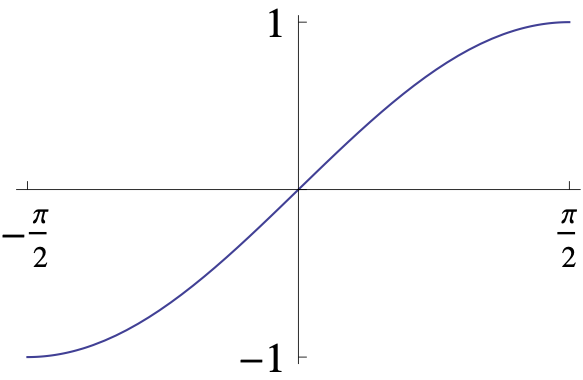
\includegraphics[width=2.60417in,height=\textheight]{./images/pplot1.png}

}

\caption{\label{fig-sinefunc}The sine function on \([-\pi/2,\pi,2]\).}

\end{figure}

\leavevmode\vadjust pre{\hypertarget{exm-nq-4}{}}%
\begin{example}[]\label{exm-nq-4}

Let \(P(x,y)\) be the statement \[
\text{If $x<y$, then $\sin x < \sin y$.}
\] The domain of discourse is the closed interval
\(I=\left[-\frac{\pi}{2},\frac{\pi}{2}\right]\). Determine which of the
following statements \[
\exists x, \exists y, P(x,y) \quad
\exists x, \forall y, P(x,y) \quad
\forall x, \exists y, P(x,y) \quad
\forall x, \forall y, P(x,y)
\] are true and which are false.

\end{example}

\begin{solution}

The first statement \(\exists x\in I, \exists y\in I, P(x,y)\) is true.
To see this simply let \(x=0\) and \(y=\pi/2\) because \(0<1\) and
\(\sin 0=0<1 =\sin \pi/2\).

The second statement
\(\exists x\in \mathbb{R}, \forall y\in \mathbb{R}, P(x,y)\) is true. To
see this let \(x=-\pi/2\), and then notice that
\(\forall y\in I, P(-\pi/2,y)\) is a true statement. That is, \[
\forall y\in I, \text{ if $-\frac{\pi}{2}<y$, then $-1<\sin y$}
\] is true. Recall the graph of the sine function restricted to the
domain of \(I\) (see Figure~\ref{fig-sinefunc}).

The third statement \(\forall x\in I, \exists y\in I, P(x,y)\) is true.
We can not prove this statement is true with one value for \(x\). Let
\(x\in I\) be an arbitrary element in \(I\). Now that \(x\) is given we
can set \(y=x\). Then \(P(x,y)\) is a true implication since it has a
false hypothesis.

The fourth statement \(\forall x\in I, \forall y\in I, P(x,y)\) is true.
Again we can not prove this statement is true with one value for \(x\).
Moreover, for any given value of \(x\), the value of \(y\) must also be
arbitrary. Let \(x\in I\) be an arbitrary element in \(I\). If
\(y\leq x\), then the implication \(P(x,y)\) is true by a false
hypothesis; and thus the statement
\(\forall x\in I, \exists y\in I, P(x,y)\) is true in this case. If
\(x<y\), then the hypothesis in the implication \(P(x,y)\) is true, but
in fact the conclusion in \(P(x,y)\) is also true since the sine
function is increasing on \(I\). Therefore, no matter what \(x\) in
\(I\) is given we see that \(P(x,y)\) is true for all \(y\) in \(I\).

\end{solution}

\hypertarget{inference-rules-for-quantified-statements}{%
\section{Inference Rules for Quantified
Statements}\label{inference-rules-for-quantified-statements}}

Before we begin proving theorems, we need to discuss the inference rules
for quantified statements. However, before we do so, the reader is
encourage to complete Exercise~\ref{exr-incidaxioms}, that is, write out
each incidence axiom in symbolic form and also write the negation of
each one in both symbolic and English form.

Suppose that \(\exists x\in U\), \(P(x)\) is true, where \(U\) is the
domain of discourse. By Definition~\ref{def-existential-quantifier},
\(P(x)\) is true for some \(x\) in \(U\). Thus, there exists \(c\in U\)
such that \(P(c)\) is true. Hence we have shown that the argument \[
\begin{array}{l} 
\exists x, P(x)
\\ \hline
\therefore \, \text{$P(c)$ for some element $c\in U$} 
\end{array} 
\] is valid. Now suppose that \(\forall x\in U\), \(P(x)\) is true. By
Definition~\ref{def-uniqueness-quantifier}, \(P(x)\) is true for every
\(x\) in \(U\). In particular, if \(c\in U\), then \(P(c)\) is true.
Hence we have shown that the argument \[
\begin{array}{l} 
\forall x, P(x)
\\ \hline
\therefore \, \text{$P(c)$ if $c\in U$}
\end{array}
\] is valid. The reader should write careful arguments to justify the
other two inference rules. All four are listed below.

\hypertarget{tbl-inference-rules}{}
\begin{longtable}[]{@{}
  >{\raggedright\arraybackslash}p{(\columnwidth - 2\tabcolsep) * \real{0.5000}}
  >{\raggedright\arraybackslash}p{(\columnwidth - 2\tabcolsep) * \real{0.5000}}@{}}
\caption{\label{tbl-inference-rules}Inference Rules for
Universe}\tabularnewline
\toprule()
\begin{minipage}[b]{\linewidth}\raggedright
Inference Rules for Universe \(U\)
\end{minipage} & \begin{minipage}[b]{\linewidth}\raggedright
Name
\end{minipage} \\
\midrule()
\endfirsthead
\toprule()
\begin{minipage}[b]{\linewidth}\raggedright
Inference Rules for Universe \(U\)
\end{minipage} & \begin{minipage}[b]{\linewidth}\raggedright
Name
\end{minipage} \\
\midrule()
\endhead
\(\begin{array}{l} \forall x, P(x) \\ \hline \therefore \, \text{$P(c)$ if $c\in U$} \end{array}\)
& Universal instantiation \\
\(\begin{array}{l} P(c) \text{ for an arbitrary $c\in U$} \\ \hline \therefore \, \forall x, P(x) \end{array}\)
& Universal generalization \\
\(\begin{array}{l} \exists x, P(x) \\ \hline \therefore \, \text{$P(c)$ for some element $c\in U$} \end{array}\)
& Existential instantiation \\
\(\begin{array}{l} P(c) \text{ for some element $c\in U$} \\ \hline \therefore \, \exists x, P(x) \end{array}\)
& Existential generalization \\
\bottomrule()
\end{longtable}

\hypertarget{exercises-1}{%
\section{Exercises}\label{exercises-1}}

\leavevmode\vadjust pre{\hypertarget{exr-forall-negation-for-each-statement}{}}%
\begin{exercise}[]\label{exr-forall-negation-for-each-statement}

Write the negation for each statement.

\begin{enumerate}
\def\labelenumi{\arabic{enumi}.}
\tightlist
\item
  \(\forall x, p(x) \land q(x)\)
\item
  \(\forall x, p(x)\lor q(x)\)
\item
  \(\forall x, p(x)\rightarrow q(x)\)
\item
  \(\forall x, p(x)\leftrightarrow q(x)\)
\item
  \(\forall x, \neg p(x)\)
\end{enumerate}

\end{exercise}

\leavevmode\vadjust pre{\hypertarget{exr-exists-negation-for-each-statement}{}}%
\begin{exercise}[]\label{exr-exists-negation-for-each-statement}

Write the negation for each statement.

\begin{enumerate}
\def\labelenumi{\arabic{enumi}.}
\tightlist
\item
  \(\exists x, p(x) \land q(x)\)
\item
  \(\exists x, p(x)\lor q(x)\)
\item
  \(\exists x, p(x)\rightarrow q(x)\)
\item
  \(\exists x, p(x)\leftrightarrow q(x)\)
\item
  \(\exists x, \neg p(x)\)
\end{enumerate}

\end{exercise}

Let \(\mathbb{N}\), \(\mathbb{Z}\), \(\mathbb{Q}\), \(\mathbb{R}\), and
\(\mathbb{C}\) denote the natural numbers, integers, the rational
numbers, the real numbers and the complex numbers, respectively.

\leavevmode\vadjust pre{\hypertarget{exr-exists-true-false}{}}%
\begin{exercise}[]\label{exr-exists-true-false}

Decide which of the following propositions are true and which are false.

\begin{enumerate}
\def\labelenumi{\arabic{enumi}.}
\tightlist
\item
  \(\exists \ x\in \mathbb{Q}, x^3+3=0.\)
\item
  \(\exists \ x\in \mathbb{R}, x^3+3=0.\)
\item
  \(\exists \ x\in \mathbb{C}, x^3+3=0.\)
\item
  \(\exists! \ x\in \mathbb{Q}, x^3+3=0.\)
\item
  \(\exists! \ x\in \mathbb{R}, x^3+3=0.\)
\item
  \(\exists! \ x\in \mathbb{C}, x^3+3=0.\)
\end{enumerate}

\end{exercise}

\leavevmode\vadjust pre{\hypertarget{exr-propositions-are-true-and-which-are-false}{}}%
\begin{exercise}[]\label{exr-propositions-are-true-and-which-are-false}

Decide which of the following propositions are true and which are false.

\begin{enumerate}
\def\labelenumi{\arabic{enumi}.}
\tightlist
\item
  \(\forall \ x\in \mathbb{N}, \exists \ y\in \mathbb{N}, x\leq y\)
\item
  \(\forall \ x\in \mathbb{Z}, \exists \ y\in \mathbb{Z}, x\leq y\)
\item
  \(\exists \ x\in \mathbb{Q}, \exists \ y\in \mathbb{N}, x\leq y\)
\item
  \(\exists \ x\in \mathbb{N}, \forall \ y\in \mathbb{N}, x\leq y\)
\item
  \(\forall \ x\in \mathbb{Z}, \forall \ y\in \mathbb{Z}, x\leq y\)
\item
  \(\exists \ x\in \mathbb{Q}, \forall \ y\in \mathbb{N}, x\leq y\)
\end{enumerate}

\end{exercise}

\leavevmode\vadjust pre{\hypertarget{exr-symbolically-with-the-quantifiers-explicit}{}}%
\begin{exercise}[]\label{exr-symbolically-with-the-quantifiers-explicit}

Rewrite the following propositions symbolically with the quantifiers
explicit and in the correct place.

\begin{enumerate}
\def\labelenumi{\arabic{enumi}.}
\tightlist
\item
  For every two distinct points \(A\) and \(B\) there exists a unique
  line \(l\) incident with \(A\) and \(B\).
\item
  For every line \(l\) there exist at least two distinct points incident
  with \(l.\)
\item
  There exist three distinct points with the property that no line is
  incident with all three of them.
\end{enumerate}

\end{exercise}

\leavevmode\vadjust pre{\hypertarget{exr-write-negation-in-symbols-words}{}}%
\begin{exercise}[]\label{exr-write-negation-in-symbols-words}

If the statement is written in symbols, then rewrite the statement using
words; and conversely. For each also write its negation in both symbols
and words.

\begin{enumerate}
\def\labelenumi{\arabic{enumi}.}
\tightlist
\item
  \((\exists \, x\in \mathbb{Z})(\forall \, y\in \mathbb{Z})(x+y=0)\)
\item
  There exists an integer \(x\) such that for all real numbers \(y\) the
  sum of \(x\) and \(y\) is zero.
\item
  There exists an integer \(y\) such that for all rational numbers \(x\)
  the sum of \(x\) and \(y\) is zero.
\item
  There exists a natural number \(x\) such that for all integers \(y\)
  the sum of \(x\) and \(y\) is zero.
\item
  There exists an natural number \(y\) such that for all natural numbers
  \(x\) the sum of \(x\) and \(y\) is zero.
\item
  \((\forall \, x\in \mathbb{N})(\exists \, y\in \mathbb{N})(x y=x)\)
\item
  There exists an integer \(x\) such that for all real numbers \(y\) the
  product of \(x\) and \(y\) is \(x\).
\item
  There exists an integer \(y\) such that for all real numbers \(x\) the
  product of \(x\) and \(y\) is \(x\).
\item
  There exists a natural number \(x\) such that for all integers \(y\)
  the product of \(x\) and \(y\) is \(x\).
\item
  There exists an natural number \(y\) such that for all rational
  numbers \(x\) the product of \(x\) and \(y\) is \(x\).
\item
  Given any two distinct real numbers, some rational number lies
  strictly between them.
\item
  \(\forall \, x,y\in \mathbb{R}, (x\neq y\rightarrow \exists \, z\in \mathbb{Q}, x<z<y)\)
\item
  \(\exists \, x,y\in \mathbb{R}, (x\neq y\rightarrow \exists \, z\in \mathbb{Q}, x<z<y)\)
\item
  \(\exists \, x,y\in \mathbb{R}, (x\neq y\rightarrow \forall \, z\in \mathbb{Q}, x<z<y)\)
\item
  \(\forall \, x,y\in \mathbb{R}, (x\neq y\rightarrow \forall \, z\in \mathbb{Q}, x<z<y)\)
\item
  \(\exists \, x,y\in \mathbb{R}, (x\neq y \rightarrow \exists \, z\in \mathbb{Q}, x<z<y)\)
\item
  \((\exists \, x\in \mathbb{Z})(\forall \, y\in \mathbb{Q})(x+y=0)\)
\item
  \((\forall \, y\in \mathbb{Z})(\exists \, x\in \mathbb{Z})(x+y=0)\)
\item
  \((\forall \, x\in \mathbb{N})(\exists \, y\in \mathbb{N})(x y=x)\)
\item
  \((\exists \, y\in \mathbb{N})(\forall \, x\in \mathbb{N})(x y=x)\)
\item
  \((\forall \, x\in \mathbb{N})(\exists \, y\in \mathbb{N})(x=y-7)\)
\item
  \((\exists \, y\in \mathbb{N})(\forall \, x\in \mathbb{N})(x=y-7)\)
\item
  \((\forall \, y\in \mathbb{N})(\forall \, x\in \mathbb{N})(y=x-7)\)
\item
  \((\exists \, x\in \mathbb{N})(\exists \, y\in \mathbb{N})(y=x-7)\)
\item
  For all integers \(x\) and \(y\), the numbers \(x y\) and \(y x\) are
  equal.
\item
  Given any real number \(x,\) there exists a natural number \(n\) such
  that \(x<n\)
\item
  Given any real number \(x,\) there exists a natural number \(y\) such
  that \(x+y=0.\)
\item
  Given any nonnegative real number \(x,\) there exists a natural number
  \(y\) such that \(y^2=x.\)
\item
  Given any nonzero real number \(x,\) there exists a natural number
  \(y\) such that \(x y=1.\)
\item
  There exists a smallest natural number.
\item
  There is no largest integer.
\item
  Given any two distinct real numbers, some rational number lies
  strictly between them.
\item
  Given any positive real number \(\epsilon ,\) there exists a natural
  number \(k\) such that \(\frac{1}{n} < \epsilon\) whenever \(n\) is a
  natural number greater than \(k.\)
\item
  For each real number \(\epsilon ,\) if \(\epsilon >0\) then there
  exists a positive real number \(\delta\) such that for each number
  \(x,\) if \(|x-2|<\delta\) then \(\left|x^2-4\right|<\epsilon .\)
\end{enumerate}

\end{exercise}

\leavevmode\vadjust pre{\hypertarget{exr-nqlab}{}}%
\begin{exercise}[]\label{exr-nqlab}

Finish the proof of Theorem~\ref{thm-thmnqlab}.

\end{exercise}

\bookmarksetup{startatroot}

\hypertarget{mathematical-proofs}{%
\chapter{Mathematical Proofs}\label{mathematical-proofs}}

In addition, proofs can help us to understand complicated concepts. By
breaking down an argument into small, manageable steps, we can see how
each piece fits together to form a larger whole.

Finally, proofs can be aesthetically pleasing. There is a certain beauty
in a well-constructed argument, just as there is beauty in a finely
crafted piece of art.

We now discuss valid arguments, inference rules, and various methods of
proof including direct proofs, indirect proofs, proof by contrapositive,
and proof by cases.

An \index{argument} \textbf{argument} is defined as a statement \(q\)
being asserted as a consequence of some list of statements
\(p_1, p_2, ...,p_k\). The statements \(p_1, p_2, ..,p_k\) are called
the \index{premises} \textbf{premises} (or \index{hypothesis})
\textbf{hypothesis} of the argument; and the statement \(q\) is called
the \index{conclusion} \textbf{conclusion}.

\leavevmode\vadjust pre{\hypertarget{def-valargu}{}}%
\begin{definition}[]\label{def-valargu}

A statement \(q\) is called a \index{propositional consequence}
\textbf{propositional consequence} of statements \(p_1, p_2, ..., p_k\)
if and only if the single statement
\((p_1 \land p_2 \land \cdots \land p_k) \rightarrow q\) is a tautology.

\end{definition}

\leavevmode\vadjust pre{\hypertarget{exm-test-validity}{}}%
\begin{example}[]\label{exm-test-validity}

Test the validity of the following arguments.

\[\begin{array}{ccc} 
\begin{array}{l} 
p \longleftrightarrow q \\
q \lor r  \\ 
\neg \, r \\ \hline
\therefore \, \neg \, p 
\end{array}
& \qquad &
\begin{array}{l}
p \lor q \\
\neg \, q \rightarrow r \\ 
\neg \, p \lor \neg \, r \\ \hline
\therefore \, \neg \, p
\end{array}
\end{array}\]

\end{example}

\begin{solution}

By Definition~\ref{def-valargu}, the arguments can be shown to be valid
or not by constructing a truth table for the following statements

\begin{enumerate}
\def\labelenumi{\arabic{enumi}.}
\tightlist
\item
  \([(p \longleftrightarrow q)\land (q \lor r ) \land (\neg \, r )] \longleftrightarrow (\neg p)\)
\item
  \([(p \lor q)\land (\neg \, q \rightarrow r)\land (\neg \, p \lor \neg \, r)] \longrightarrow (\neg p)\)
\end{enumerate}

and determining whether or not these are tautologies. The reader should
verify that the first statement is not a tautology, and so the argument
in (a) is not valid. What about the second statement?

\end{solution}

\hypertarget{logical-discourse}{%
\section{Logical Discourse}\label{logical-discourse}}

The pattern of logical discourse goes as follows:

\begin{itemize}
\tightlist
\item
  A collection of primitive (undefined terms) is given.
\item
  A collection of axioms (unproven statements) about the primitive terms
  is also given.\\
\item
  Then all of the terms of the discourse are defined by means of the
  primitive terms or by previously defined terms that were defined using
  primitive terms.\\
\item
  All other statements in the system are logically deduced from the
  axioms. These are the theorems of the system.
\end{itemize}

In mathematical exposition, we often communicate by distinguishing
different types of theorems. For example, a theorem is sometimes called
a \index{result} \textbf{result}. There is an air of humility in calling
a theorem merely a result. Other alternatives to \index{theorem}
\textbf{theorem} are listed below.

\textbf{Fact}. A very minor theorem, but important enough to number and
refer to latter, i.e., the statement \(1+1=2\) is a fact.

\textbf{Proposition}. Also a minor theorem, but more important (usually
more general) than a fact --but not as prestigious as a theorem.

\textbf{Lemma}. Often a technical theorem, which is used to help prove
another more important theorem. Stating lemmas, before proving a
difficult complicated theorem, is functional.

\textbf{Claim}. Similar to lemma but less formal. A claim will often be
referred to only a small number of times, whereas a lemma may be
referenced many times and is a useful result in itself. For example,
stating a claim inside the proof theorem is a great way to help organize
key steps in a proof.

\textbf{Corollary}. An important enough result to state on its own whose
proof requires a previously proved theorem as its main step.

\hypertarget{writing-proofs}{%
\section{Writing Proofs}\label{writing-proofs}}

\hypertarget{direct-proofs}{%
\subsection{Direct Proofs}\label{direct-proofs}}

Basically, direct proofs are proofs that do not use the Law of Excluded
middle tautology. In each of the following examples, we use inference
rules to write a proof in column format -- and we also write a paragraph
proof.

\leavevmode\vadjust pre{\hypertarget{exm-direct-proofs}{}}%
\begin{example}[]\label{exm-direct-proofs}

Given the three previously proven theorems:

\begin{itemize}
\tightlist
\item
  Theorem 1: \(p\rightarrow q\),
\item
  Theorem 2: \(q\rightarrow r\), and
\item
  Theorem 3: \(r\rightarrow s\).
\end{itemize}

We can now prove the next theorem. \[
\text{Theorem: If $p$ then $s$.}
\]

\end{example}

\begin{solution}

We begin with a column proof.

\begin{longtable}[]{@{}lll@{}}
\toprule()
Conclusions & Justifications & \\
\midrule()
\endhead
\(p\) & premise & \\
\(p\rightarrow q\) & theorem 1 & \\
\(q\) & steps 1 and 2, modus ponens & \\
\(q\rightarrow r\) & theorem 2 & \\
\(r\) & steps 3 and 4, modus ponens & \\
\(r\rightarrow s\) & theorem 3 & \\
\(s\) & steps 5 and 6, modus ponens & \\
\bottomrule()
\end{longtable}

We end with a paragraph proof.

\begin{quote}
Assume \(p\). By Theorem 1, we know \(q\), and so by Theorem 2, we now
have \(r\). Hence by Theorem 3, we have \(s\) as needed.
\end{quote}

\end{solution}

\leavevmode\vadjust pre{\hypertarget{exm-proof-example}{}}%
\begin{example}[]\label{exm-proof-example}

Prove: if \(p\lor q\) and \(\neg \, q\), then \(p\).

\end{example}

\begin{solution}

We begin with a column proof.

\begin{longtable}[]{@{}ll@{}}
\toprule()
Conclusions & Justifications \\
\midrule()
\endhead
\(\neg q\) & premise \\
\(p\lor q\) & premise \\
\(p\) & disjunctive syllogism \\
\bottomrule()
\end{longtable}

We end with a paragraph proof:

\begin{quote}
Assume \(\neg q\) and \(p\lor q\). We can not have \(q\) and \(\neg q\),
thus \(p\) follows immediately.
\end{quote}

\end{solution}

\leavevmode\vadjust pre{\hypertarget{exm-proof-example-2}{}}%
\begin{example}[]\label{exm-proof-example-2}

Assume the following:

\begin{itemize}
\tightlist
\item
  Definition: \(a\) is said to be \(b\) iff \(r\rightarrow s\),
\item
  Axiom 1: \(r\rightarrow q\),
\item
  Theorem 1: If \(a\) is \(c\) then \(q\rightarrow t\),
\item
  Theorem 2: \(t\rightarrow s\).
\end{itemize}

Prove the following theorem. \[
\text{Theorem: If $a$ is $c$ then $a$ is $b.$}
\]

\end{example}

\begin{solution}

We begin with a column proof.

\begin{longtable}[]{@{}ll@{}}
\toprule()
Conclusions & Justifications \\
\midrule()
\endhead
\(a\) is \(c\) & premise \\
if \(a\) is \(c\) then \(q\rightarrow t\) & theorem 1 \\
\(q\rightarrow t\) & steps 2 and 3, modus ponens \\
\(r\) & premise \\
\(r\rightarrow q\) & axiom 1 \\
\(q\) & steps 4 and 5, modus ponens \\
\(t\) & steps 3 and 6, modus ponens \\
\(t\rightarrow s\) & theorem 2 \\
\(s\) & steps 7 and 8, modus ponens \\
\(r\rightarrow s\) & steps 4 through 9 \\
\(a \text{ is } b\) & definition of \(a\) is \(b\) \\
\bottomrule()
\end{longtable}

We end with a paragraph proof:

\begin{quote}
Assume \(a\) is \(c\). By Theorem 1, we have \(q\rightarrow t\). To
prove that \(a\) is \(b\) we assume \(r\). Then by Axiom 1, we have
\(q\), which now yields \(t\). By Theorem 2, it follows that \(s\).
Therefore we have shown \(r\rightarrow s\) as needed.
\end{quote}

\end{solution}

\hypertarget{indirect-proofs}{%
\subsection{Indirect Proofs}\label{indirect-proofs}}

\leavevmode\vadjust pre{\hypertarget{exm-indirect-proofs}{}}%
\begin{example}[]\label{exm-indirect-proofs}

Given the two previously proven theorems:

\begin{itemize}
\tightlist
\item
  Theorem 1: \(\neg q\rightarrow r\),
\item
  Theorem 2: If \(r\) then either \(\neg p\) or \(q\).
\end{itemize}

Prove the following theorem. \[
\text{Theorem: $p\rightarrow q.$}
\]

\end{example}

\begin{solution}

We begin with a column proof.

\begin{longtable}[]{@{}
  >{\raggedright\arraybackslash}p{(\columnwidth - 2\tabcolsep) * \real{0.5000}}
  >{\raggedright\arraybackslash}p{(\columnwidth - 2\tabcolsep) * \real{0.5000}}@{}}
\toprule()
\begin{minipage}[b]{\linewidth}\raggedright
Conclusions
\end{minipage} & \begin{minipage}[b]{\linewidth}\raggedright
Justifications
\end{minipage} \\
\midrule()
\endhead
\(p\) & premise \\
\(q \lor \neg q\) & excluded middle \\
\(\neg\) & premise \\
\(\neg q\rightarrow r\) & theorem 1 \\
\(r\) & steps 3 and 4, modus ponens \\
\(r\rightarrow (\neg p \lor q)\) & theorem 2 \\
\(\neg p \lor q\) & steps 5 and 6, modus ponens \\
\(p\land \neg q\) & steps 1 and 3 \\
\(\neg(\neg p)\land \neg q\) & double negation \\
\(\neg (\neg p \lor q)\) & step 9, De Morgan \\
\((\neg p \lor q) \land \neg (\neg p \lor q)\) & steps 7 and 10,
contradiction \\
\(q\) & steps 3 and 11, indirect proof \\
\bottomrule()
\end{longtable}

We end with a paragraph proof:

\begin{quote}
Assume \(p\). Suppose \(\neg q\) for otherwise we are finished. Then
\(r\) by Theorem 1. By hypothesis we cannot have \(\neg p\), and so by
Theorem 2, we have \(q\) as needed.
\end{quote}

\end{solution}

\leavevmode\vadjust pre{\hypertarget{exm-indirect-proofs}{}}%
\begin{example}[]\label{exm-indirect-proofs}

Prove: if \(p\leftrightarrow q\) and \(q\rightarrow \neg \, p\), then
\(\neg \, p\).

\end{example}

\begin{solution}

We begin with a column proof.

\begin{longtable}[]{@{}
  >{\raggedright\arraybackslash}p{(\columnwidth - 2\tabcolsep) * \real{0.5000}}
  >{\raggedright\arraybackslash}p{(\columnwidth - 2\tabcolsep) * \real{0.5000}}@{}}
\toprule()
\begin{minipage}[b]{\linewidth}\raggedright
Conclusions
\end{minipage} & \begin{minipage}[b]{\linewidth}\raggedright
Justifications
\end{minipage} \\
\midrule()
\endhead
\(p\leftrightarrow q\) & premise \\
\((p\rightarrow q) \land (q\rightarrow p\) & definition of
\(\leftrightarrow\) \\
\(p\rightarrow q\) & simplification \\
\(q\rightarrow \neg p\) & premise \\
\(p\lor \neg p\) & excluded middle \\
\(p\) & premise \\
\(q\) & steps 3 and 6, modus ponens \\
\(\neg p\) & steps 4 and 7, modus ponens \\
\(p\land \neg p\) & steps 6 and 9, contradiction \\
\(\neg p\) & steps 5-9, indirect proof \\
\bottomrule()
\end{longtable}

We end with a paragraph proof:

\begin{quote}
Assume for a contradiction \(p\). Since \(p\) and \(q\) are equivalent,
we have \(q\). By hypothesis, we then have \(\neg p\). Since \(\neg p\)
and \(p\) is a contradiction, our original premise of \(p\) can not
happen. Whence \(\neg p\).
\end{quote}

\end{solution}

\leavevmode\vadjust pre{\hypertarget{exm-indirect-proofs-2}{}}%
\begin{example}[]\label{exm-indirect-proofs-2}

Assume the following:

\begin{itemize}
\tightlist
\item
  Axiom 1: \(p\) implies either \(r\) or \(s\),
\item
  Theorem 1: \(y\rightarrow \neg p\),
\item
  Theorem 2: \(r\rightarrow x\),
\item
  Theorem 3: \(s\rightarrow y\),
\item
  Theorem 4: \(x\rightarrow q\).
\end{itemize}

Prove the following theorem. \[
\text{Theorem: $p\rightarrow q.$}
\]

\end{example}

\begin{solution}

We begin with a column proof.

\begin{longtable}[]{@{}ll@{}}
\toprule()
Conclusions & Justifications \\
\midrule()
\endhead
\(p\) & premise \\
\(p\rightarrow (r\lor s)\) & axiom 1 \\
\(r\lor s\) & steps 1 and 2, modus ponens\} \\
\(s\) & premise \\
\(s\rightarrow y\) & theorem 3 \\
\(y\) & steps 4 and 5, modus ponens \\
\(y\rightarrow \neg p\) & theorem 1 \\
\(\neg p\) & steps 6 and 7, modus ponens \\
\(p\land \neg p\) & steps 1 and 8, contradiction \\
\(\neg s\) & steps 4-9, indirect proof \\
\(r\) & steps 3 and 10, disjunctive syllogism \\
\(r\rightarrow x\) & theorem 2 \\
\(x\) & steps 11 and 12, modus ponens \\
\(x\rightarrow q\) & theorem 4 \\
\(q\) & steps 13 and 14, modus ponens \\
\bottomrule()
\end{longtable}

We end with a paragraph proof:

\begin{quote}
Assume \(p\). If we have \(s\), then by Theorem 3, we have \(y\); yet by
Theorem 1 this yields \(\neg p\). Since we can not have both \(\neg p\)
and \(p\) we see that we can not have \(s\). Hence we have \(\neg s\).
By Axiom 1, we must have \(r\). By Theorem 2, we now have \(x\), and so
by Theorem 4, we conclude with \(q\) as needed.
\end{quote}

\end{solution}

\hypertarget{proof-by-contrapositive}{%
\subsection{Proof by Contrapositive}\label{proof-by-contrapositive}}

\leavevmode\vadjust pre{\hypertarget{exm-proof-by-contrapositive}{}}%
\begin{example}[]\label{exm-proof-by-contrapositive}

Assume the following:

\begin{itemize}
\tightlist
\item
  Axiom 1: \(p\rightarrow \neg y\).
\item
  Axiom 2: \(\neg q\rightarrow r\).
\item
  Theorem 1: \(p\rightarrow \neg z\).
\item
  Theorem 2: \(x\rightarrow \text{ either } q \text{ or } z.\).
\item
  Theorem 3: \(r\rightarrow \text{ either } x \text{ or } y\). \[
  \text{Theorem: $\neg p\rightarrow \neg q.$}
  \]
\end{itemize}

\end{example}

\begin{solution}

We prove the (logical equivalent) contrapositive statement
\(p\rightarrow q\).\\
We begin with a column proof.

\begin{longtable}[]{@{}ll@{}}
\toprule()
Conclusions & Justifications \\
\midrule()
\endhead
\(p\) & premise \\
\(p\rightarrow \neg y\) & axiom 1 \\
\(\neg y\) & steps 1 and 2, modus ponens \\
\(q \lor \neg q\) & excluded middle \\
\(\neg q\) & premise \\
\(\neg q\rightarrow r\) & axiom 2 \\
\(r\) & steps 5 and 6, modus ponens \\
\(r\rightarrow x \lor y\) & theorem 3 \\
\(x \lor y\) & steps 7 and 8, modus ponens \\
\(x\) & steps 3 and 9, disjunctive syllogism \\
\(x\rightarrow q\lor z\) & theorem 2 \\
\(q\lor z\) & steps 10 and 11, modus ponens \\
\(z\) & premise \\
\(p\rightarrow \neg z\) & theorem 1 \\
\(z \rightarrow \neg p\) & contrapositive \\
\(\neg p\) & steps 13 and 15, modus ponens \\
\(p\land \neg p\) & steps 1 and 16, contradiction \\
\(\neg z\) & steps 13 and 17, indirect proof \\
\(q\) & steps 12 and 18, disjunctive syllogism \\
\(\neg (\neg q)\) & steps 5 and 19, contradiction \\
\(q\) & steps 4 and 20, disjunctive syllogism \\
\bottomrule()
\end{longtable}

We end with a paragraph proof:

\begin{quote}
Assume \(p\). Then by Axiom 1 we have \(\neg y\). Assume for a
contradiction that \(\neg q\). Then by Axiom 2 we have \(r\), and so
either \(x\) or \(y\) by Theorem 3. In case we have \(x\), then by
Theorem 2 we have \(z\). Now \(\neg p\) follows by Theorem 1 and so this
contradiction show that \(x\) can not happen. Hence \(y\) follows. Yet
now we have \(y\) and \(\neg y\) and so it fact we cannot have
\(\neg q\). Therefore \(q\) as needed.
\end{quote}

\end{solution}

\hypertarget{proof-by-cases}{%
\subsection{Proof by Cases}\label{proof-by-cases}}

\leavevmode\vadjust pre{\hypertarget{exm-proof-by-cases}{}}%
\begin{example}[]\label{exm-proof-by-cases}

Assume the following:

\begin{itemize}
\tightlist
\item
  Theorem 1: \(r\rightarrow \, \neg p\),
\item
  Theorem 2: \(s\rightarrow \, \neg p\),
\item
  Theorem 3: A complete set of logical possibilities is: \(r, s,\) and
  \(q;\) that is, one of the statements \(r, s,\) and \(q\) is true and
  only one.
\end{itemize}

Prove the following theorem. \[
\text{Theorem: If $p$ then $q$.}
\]

\end{example}

\begin{solution}

We begin with a column proof.

\begin{longtable}[]{@{}ll@{}}
\toprule()
Conclusions & Justifications \\
\midrule()
\endhead
\(p\) & premise \\
one and only one holds: \(r, s, q\) & theorem 3 \\
\(r\) & premise (case 1) \\
\(r\rightarrow \neg p\) & theorem 1 \\
\(\neg p\) & steps 3 and 4, modus ponens \\
\(p \land \neg p\) & steps 1 and 5, contradiction \\
\(\neg r\) & steps 3 and 6, indirect proof \\
\(s\) & premise (case 2) \\
\(s\rightarrow \neg p\) & theorem 2 \\
\(\neg p\) & steps 8 and 9, modus ponens \\
\(p \land \neg p\) & steps T and 10, contradiction \\
\(\neg s\) & steps 8 and 11, indirect proof \\
\(q\) & step 2 \\
\bottomrule()
\end{longtable}

We end with a paragraph proof:

\begin{quote}
Assume \(p\). By Theorem 3, there are exactly three cases two consider.
If \(r\), then we have \(\neg p\) by Theorem 1 which is contrary to
hypothesis. Similarly, \(s\) is contrary to hypothesis. Hence we have
\(q\) as needed.
\end{quote}

\end{solution}

We end this section with a short discussion on how you might have seen
these types of arguments (proofs) before in precalculus. We will
demonstrate three ways to prove the statement: \[
\text{If  $x^3-x^2+x-1=0$, then $x=1$.}
\]

\begin{itemize}
\tightlist
\item
  (\textbf{Direct Proof}) Assume \(x^3-x^2+x-1=0\). Then
  \((x-1)(x^2+1)=0\), which implies that either \(x-1=0\) or
  \(x^2+1=0\). But we know that \(x^2+1\neq 0\) (since \(x\) is real),
  and so it must be the case that \(x-1\)=0. Hence \(x=1\).
\item
  (\textbf{Proof by Contrapositive}) Assume \(x\neq 1\). Then
  \(x-1\neq 0\). Also, since \(x\) is real, \(x^2+1\neq 0\). It follows
  that \((x-1)(x^2+1)\neq 0\). Upon multiplication we obtain the result
  \(x^3-x^2+x-1\neq 0\).
\item
  (\textbf{Proof by Contradiction}) Suppose \(x^3-x^2+x-1\) and assume
  for a contradiction that \(x\neq 1\). Then \(x-1\neq 0\). Since
  \(x^4-x^2+x-1=(x-1)(x^2+1))\) and \(x-1\neq 0\), it must be that
  \(x^2+1=0\). This is a contradiction because \(x\) is a real number.
  Therefore, we conclude \(x=1\).
\end{itemize}

\hypertarget{axiomatic-systems}{%
\section{Axiomatic Systems}\label{axiomatic-systems}}

In this chapter we discuss axiomatic systems and inference rules for
quantified statements. To give an example of this process, we carry out
a simple logical discourse for incidence geometry involving points,
lines, and incidence.

An \index{axiomatic} \textbf{axiomatic} (or \index{formal}
\textbf{formal}) system must contain a set of technical terms that are
deliberately chosen as undefined, called \index{undefined terms}
\textbf{undefined terms}, and are subject to the interpretation (an
intuition) of the reader. All other technical terms of the system are
ultimately defined by means of the undefined terms, and are called
\index{definitions} \textbf{definitions}. An axiomatic system contains a
set of statements, dealing with undefined terms and definitions, that
are chosen to remain unproved, and are called \index{axioms}
\textbf{axioms}.

\hypertarget{incidence-geometry}{%
\subsection{Incidence Geometry}\label{incidence-geometry}}

Below is an example of a simple axiomatic system where the terms
\emph{point}, \emph{line}, and \emph{incidence} only have the meaning
given by a small collection of axioms.

We assume that we have a collection of points and a collection of lines.
The only other assumptions we make about these points and lines, and
their behavior, is given solely by the axioms.

\begin{quote}
The goal is not to say what a point is or what a line is, but rather to
discover how they behave, relatively to each other.
\end{quote}

\textbf{Axioms}. Let \index{point} \textbf{point}, \index{line}
\textbf{line}, and \index{incidence} \textbf{incidence} be undefined
terms. Collectively the following three axioms are called the
\index{Incidence Axioms} \textbf{Incidence Axioms}.

\textbf{(A1)} For every two distinct points \(A\) and \(B\) there exists
a unique line \(l\) incident with \(A\) and \(B\), and is denoted by
\(l(A,B)\).

\textbf{(A2)} For every line \(l\) there exist at least two distinct
points incident with \(l.\)

\textbf{(A3)} There exist three distinct points with the property that
no line is incident with all three of them.

We will use the following convention: uppercase letters denote points,
i.e.~\(A\), \(B\), \ldots \(P\), \(Q\), etc, and lowercase letters
denote lines, i.e.~\(l, m, n\).

\leavevmode\vadjust pre{\hypertarget{def-collcom}{}}%
\begin{definition}[]\label{def-collcom}

Three or more points are called \index{collinear} \textbf{collinear} if
there exists a line incident with all of them. Three or more lines are
called \index{concurrent} \textbf{concurrent} if there exists a point
incident with all of them.

\end{definition}

Notice the definitions of collinear and concurrent are dual notions, in
the sense that they are defined the same way except that the roles of
point and line are interchanged. We use the terms \index{noncollinear}
\textbf{noncollinear} and \index{nonconcurrent} \textbf{nonconcurrent}
to mean not collinear and not concurrent, respectively.

Lines \(l\) and \(m\) are called \index{equal lines} \textbf{equal
lines} , denoted by \(l=m\), if every point incident with \(l\) is also
incident with \(m\), and conversely. Lines \(l\) and \(m\) are called
\index{parallel lines} \textbf{parallel lines} if \(l=m\) or if no point
is incident with both of them. The notation \(l\parallel m\) means line
\(l\) is parallel to line \(m\).

\leavevmode\vadjust pre{\hypertarget{thm-incidence1}{}}%
\begin{theorem}[]\label{thm-incidence1}

If \(l\) and \(m\) are distinct lines that are not parallel, then \(l\)
and \(m\) have a unique point in common.

\end{theorem}

\begin{figure}

{\centering 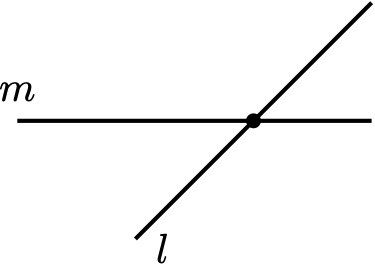
\includegraphics[width=1.5625in,height=\textheight]{./images/incidence-geometry-1-pics.png}

}

\caption{\label{fig-notpar}Unique point in common.}

\end{figure}

\begin{proof}

We begin with a column proof.

\begin{longtable}[]{@{}
  >{\raggedright\arraybackslash}p{(\columnwidth - 4\tabcolsep) * \real{0.1429}}
  >{\raggedright\arraybackslash}p{(\columnwidth - 4\tabcolsep) * \real{0.5714}}
  >{\raggedright\arraybackslash}p{(\columnwidth - 4\tabcolsep) * \real{0.2857}}@{}}
\toprule()
\begin{minipage}[b]{\linewidth}\raggedright
No.
\end{minipage} & \begin{minipage}[b]{\linewidth}\raggedright
Conclusions
\end{minipage} & \begin{minipage}[b]{\linewidth}\raggedright
Justifications
\end{minipage} \\
\midrule()
\endhead
1 & Lines \(l\) and \(m\) are distinct lines that are not parallel. &
Hypothesis \\
2 & Exactly one must hold: \(l\) and \(m\) either have no points in
common or not & Law of Excluded Middle \\
3 & There does not exists any points incident with both \(l\) and \(m\).
& Case 1 \\
4 & Lines \(l\) and \(m\) are parallel. & Definition of parallel \\
5 & \(\rightarrow\leftarrow\) & Steps 1, 4 \\
6 & Lines \(l\) and \(m\) have points in common. & Case 2 \\
7 & Exactly one must hold: lines \(l\) and \(m\) have exactly one point
in common or more. & Law of Excluded Middle \\
8 & There exists distinct points \(P\) and \(Q\) that are both incident
with both lines \(l\) and \(m\). & Case 2.1 \\
9 & \(l=m\) & Axiom 1 \\
10 & \(\rightarrow\leftarrow\) & Step 1 \\
11 & There exists exactly one point incident with lines \(l\) and \(m\).
& Case 2.2 \\
\bottomrule()
\end{longtable}

We end with a paragraph proof.

\begin{quote}
Assume \(l\) and \(m\) are distinct lines that are not parallel. By
definition of parallel lines, these lines must have at least one point
in common. If they have another point in common, then they are the same
line by Axiom 1. Therefore, they have a unique point in common.
\end{quote}

\end{proof}

\leavevmode\vadjust pre{\hypertarget{thm-incidence2}{}}%
\begin{theorem}[]\label{thm-incidence2}

There exist three distinct lines that are nonconcurrent.

\end{theorem}

\begin{figure}

{\centering 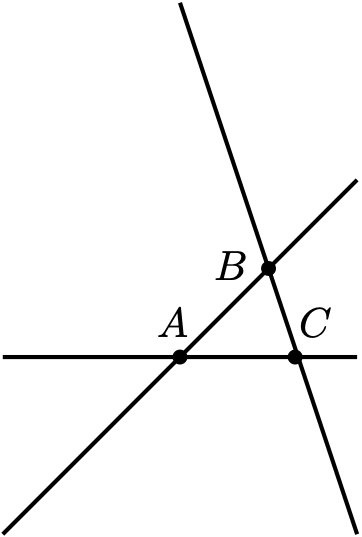
\includegraphics[width=1.5625in,height=\textheight]{./images/incidence-geometry-2-pics.png}

}

\caption{\label{fig-noncon}Nonconcurrent lines.}

\end{figure}

\begin{proof}

We begin with a column proof.

\begin{longtable}[]{@{}
  >{\raggedright\arraybackslash}p{(\columnwidth - 4\tabcolsep) * \real{0.1429}}
  >{\raggedright\arraybackslash}p{(\columnwidth - 4\tabcolsep) * \real{0.5714}}
  >{\raggedright\arraybackslash}p{(\columnwidth - 4\tabcolsep) * \real{0.2857}}@{}}
\toprule()
\begin{minipage}[b]{\linewidth}\raggedright
No.
\end{minipage} & \begin{minipage}[b]{\linewidth}\raggedright
Conclusions
\end{minipage} & \begin{minipage}[b]{\linewidth}\raggedright
Justifications
\end{minipage} \\
\midrule()
\endhead
1 & \(A\), \(B\), and \(C\) are distinct noncollinear points. & Axiom
3 \\
2 & There exists a line \(\overleftrightarrow{AB}\) incident with \(A\)
and \(B\). & Axiom 1 \\
3 & There exists a line \(\overleftrightarrow{BC}\) incident with \(B\)
and \(C\). & Axiom 1 \\
4 & There exists a line \(\overleftrightarrow{AC}\) incident with \(A\)
and \(C\). & Axiom 1 \\
5 & \(\overleftrightarrow{AB}=\overleftrightarrow{BC}\) & RAA
Hypothesis \\
6 & \(A\) is incident with \(\overleftrightarrow{BC}\) & Definition of
equality \\
7 & \(A\), \(B\), and \(C\) are collinear points. & Definition of
collinear \\
8 & \(\rightarrow\leftarrow\) & Steps 1, 7 \\
9 & \(\overleftrightarrow{AB}\neq\overleftrightarrow{BC}\) & RAA
Conclusion \\
10 & \(\overleftrightarrow{AB}=\overleftrightarrow{AC}\) & RAA
Hypothesis \\
11 & \(B\) is incident with \(\overleftrightarrow{AC}\) & Definition of
equality \\
12 & \(A\), \(B\), and \(C\) are collinear points. & Definition of
collinear \\
13 & \(\rightarrow\leftarrow\) & Steps 1, 12 \\
14 & \(\overleftrightarrow{AB}\neq\overleftrightarrow{AC}\) & RAA
Conclusion \\
15 & \(\overleftrightarrow{AC}=\overleftrightarrow{BC}\) & RAA
Hypothesis \\
16 & \(A\) is incident with \(\overleftrightarrow{BC}\) & Definition of
equality \\
17 & \(A\), \(B\), and \(C\) are collinear points. & Definition of
collinear \\
18 & \(\rightarrow\leftarrow\) & Steps 1, 17 \\
19 & \(\overleftrightarrow{AC}\neq\overleftrightarrow{BC}\) & RAA
Conclusion \\
20 & Lines \(\overleftrightarrow{AB}\), \(\overleftrightarrow{BC}\),
\(\overleftrightarrow{AC}\) are three distinct lines. & Steps 9, 14,
19 \\
21 & There exists a point \(X\) incident with all three lines
\(\overleftrightarrow{AB}\), \(\overleftrightarrow{BC}\),
\(\overleftrightarrow{AC}\). & RAA Hypothesis \\
22 & One and only one must hold: \(X=A\) or \(X\neq A\). & Law of
Excluded Middle \\
23 & \(X=A\) & Case 1 \\
24 & Point \(A\) is incident with all three lines
\(\overleftrightarrow{AB}\), \(\overleftrightarrow{BC}\), and
\(\overleftrightarrow{AC}\). & Steps 21, 23 \\
25 & \(A\), \(B\), \(C\) are collinear points. & Definition of
Collinear \\
26 & \(\rightarrow\leftarrow\) & Steps 1, 25 \\
27 & \(X\neq A\) & Case 2 \\
28 & Lines \(\overleftrightarrow{AB}\) and \(\overleftrightarrow{AC}\)
are not parallel. & Def. of Parallel Lines \\
29 & \(X=A\) & Theorem 2 \\
30 & \(\rightarrow\leftarrow\) & Steps 27, 29 \\
31 & There does not exist a point \(X\) incident with all three lines
\(\overleftrightarrow{AB}\), \(\overleftrightarrow{BC}\),
\(\overleftrightarrow{AC}\). & RAA Conclusion \\
32 & lines \(\overleftrightarrow{AB}\), \(\overleftrightarrow{BC}\),
\(\overleftrightarrow{AC}\) are nonconcurrent. & Def. of
nonconcurrent \\
\bottomrule()
\end{longtable}

We end with a paragraph proof.

\begin{quote}
By Axiom 3, there exists three distinct points \(A\), \(B\), and \(C\)
and by axiom 1, we have lines \(l(A,B)\), \(l(B,C)\), and \(l(A,C)\). If
\(l(A,B)=l(B,C)\), then points \(A\), \(B\), and \(C\) are collinear,
contrary to hypothesis. Hence \(l(A,B)\neq l(B,C)\). Similarly, it
follows \(l(B,C)\neq l(A,C)\) and \(l(A,B)\neq l(A,C)\). Thus we have
three distinct lines. Assume these lines are concurrent with point
\(X\). If \(X=A\), then \(A\) is on all three lines and again we
contradict the hypothesis. Hence \(X\neq A\), and so the nonparallel
lines \(l(A,B)\) and \(l(A,C)\) have more than one point in common. This
contradicts Theorem 2, and so \(X\) can not exist. Whence these three
distinct lines are nonconcurrent.
\end{quote}

\end{proof}

\leavevmode\vadjust pre{\hypertarget{thm-incidence4}{}}%
\begin{theorem}[]\label{thm-incidence4}

For every point, there is at least one line not passing through it.

\end{theorem}

\begin{figure}

{\centering 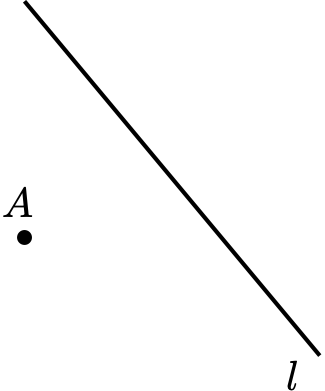
\includegraphics[width=1.5625in,height=\textheight]{./images/incidence-geometry-3-pics.png}

}

\caption{\label{fig-onelinenot}Point not on line.}

\end{figure}

\begin{proof}

We begin with a column proof.

\begin{longtable}[]{@{}
  >{\raggedright\arraybackslash}p{(\columnwidth - 4\tabcolsep) * \real{0.1429}}
  >{\raggedright\arraybackslash}p{(\columnwidth - 4\tabcolsep) * \real{0.5714}}
  >{\raggedright\arraybackslash}p{(\columnwidth - 4\tabcolsep) * \real{0.2857}}@{}}
\toprule()
\begin{minipage}[b]{\linewidth}\raggedright
No.
\end{minipage} & \begin{minipage}[b]{\linewidth}\raggedright
Conclusions
\end{minipage} & \begin{minipage}[b]{\linewidth}\raggedright
Justifications
\end{minipage} \\
\midrule()
\endhead
1 & \(A\) is a point & Hypothesis \\
2 & \(A\) is incident with every line. & RAA Hypothesis \\
3 & There exists 3 noncollinear points \(E\), \(D\), \(F\). & Axiom 3 \\
4 & There exists a line \(\overleftrightarrow{ED}\) incident with \(E\)
and \(D\). & Axiom 1 \\
5 & There exists a line \(\overleftrightarrow{DF}\) incident with \(D\)
and \(F\). & Axiom 1 \\
6 & One and only one must hold: \(A=D\) or \(A\neq D\). & Law of
Excluded Middle \\
7 & \(A\neq D\) & Case 1 \\
8 & \(A\) and \(D\) are incident with \(\overleftrightarrow{ED}\) and
\(\overleftrightarrow{DF}\). & Steps 2, 4, 5 \\
9 & \(\overleftrightarrow{ED}\)= \(\overleftrightarrow{DF}\) & Axiom
1 \\
10 & \(F\) is incident with \(\overleftrightarrow{ED}\). & Definition of
Equal Lines \\
11 & \(E\), \(D\), and \(F\) are collinear points. & Definition of
collinear \\
12 & \(\rightarrow\leftarrow\) & Steps 3 and 11 \\
13 & \(A=D\) & Case 2 \\
14 & \(D\) is incident with every line. & Steps 2, 13 \\
15 & There exists a line \(\overleftrightarrow{EF}\) incident with \(E\)
and \(F\). & Axiom 1 \\
16 & \(D\) is incident with \(\overleftrightarrow{EF}\). & Step 1 \\
17 & \(E\), \(D\), and \(F\) are collinear points. & Definition of
Collinear \\
18 & \(\rightarrow\leftarrow\) & Steps 3, 17 \\
19 & There exists a line not incident with \(A\). & RAA conclusion \\
\bottomrule()
\end{longtable}

We end with a paragraph proof.

\begin{quote}
Let \(A\) be an arbitrary point. Assume every line is incident with
\(A\). By Axiom 3, there exists three distinct points, say \(D\), \(E\),
and \(F\). Point \(A\) is not one of these points, say \(D\). By Axiom
1, we have lines \(l(E,D)\) and \(l(D,F)\). Further, since \(A\) and
\(D\) are distinct points and both are on \(l(E,D)\) and \(l(D,F)\) we
have \(l(E,D)=l(D,F)\), by Axiom 1. Hence \(E, D\), and \(F\) are
collinear. Therefore, point \(A\) is not incident with at least one
line.
\end{quote}

\end{proof}

\hypertarget{peanos-axioms}{%
\subsection{Peano's Axioms}\label{peanos-axioms}}

\textbf{Peano's Axioms} \(\mathbb{N}\) is a set with the following
properties.

\begin{itemize}
\tightlist
\item
  \(\mathbb{N}\) has a distinguished element which we call \textbf{1}.
\item
  There exists a distinguished set map \(s: \mathbb{N} \to \mathbb{N}\).
\item
  The mapping \(s\) is injective.
\item
  There does not exists an element \(n\in \mathbb{N}\) such that
  \(s(n)=1\).
\item
  If \(S\) is a subset of \(\mathbb{N}\) with the properties: \(1\in S\)
  and if \(n\in S\), then \(s(n)\in S\), then \(S=\mathbb{N}\).
\end{itemize}

We call such a set \(\mathbb{N}\) to be the set of natural numbers and
elements of this set to be natural numbers.

\leavevmode\vadjust pre{\hypertarget{thm-wdef}{}}%
\begin{theorem}[]\label{thm-wdef}

If \(n\in\mathbb{N}\) and \(n\neq 1\), then there exists a unique
\(m\in \mathbb{N}\) such that \(s(m)=n\).

\end{theorem}

\begin{proof}

Consider the subset \begin{equation}
S=\{n\in \mathbb{N} \mid n=1 \text{ or } n=s(m), \text{ for some } m\in \mathbb{N}\}.
\end{equation} By definition, \(1\in S\). If \(n\in S\), clearly
\(s(n)\in S\), again by definition of \(S\). Thus by induction, we see
that \(S=\mathbb{N}\). Further injectivity of \(s\) implies uniqueness
as claimed.

\end{proof}

By \ref{wdef}, the following definition of addition is well-defined.

\leavevmode\vadjust pre{\hypertarget{def-}{}}%
\begin{definition}[]\label{def-}

Let \emph{addition} be the operation \(+:X\times X\to X\) recursively
defined on \(y\) by \begin{equation}
x+y:=
\begin{cases}
x & \text{if $y=0$} \\
s(x+z) & \text{if $y\in s(X)$ and $y=s(z)$} \\
\end{cases}
\end{equation}

\end{definition}

Notice \(0+0=0\) and that \(x+0=x\), for all \(x\in X\).

\leavevmode\vadjust pre{\hypertarget{lem-}{}}%
\begin{lemma}[]\label{lem-}

\label{prop1} For all \(x\in X\), \(x+1=s(x)\).

\end{lemma}

\begin{proof}

Let \(x\in X\). Immediately, \(x+1=x+s(0)=s(x+0)=s(x)\).

\end{proof}

\leavevmode\vadjust pre{\hypertarget{lem-}{}}%
\begin{lemma}[]\label{lem-}

\label{prop2} For all \(x\in X\), \(0+x=x\).

\end{lemma}

\begin{proof}

We use induction on \(x\). First, \(0+1=0+s(0)=s(0+0)=s(0)=1\). Assume
that \(0+y=y\). We must show that \(0+s(y)=s(y)\). We have
\(0+s(y)=s(0+y)=s(y)\). Therefore, \(0+x=x\), for all \(x\in X\).

\end{proof}

\leavevmode\vadjust pre{\hypertarget{lem-}{}}%
\begin{lemma}[]\label{lem-}

\label{prop3} For all \(x,y\in X\), \(s(x+y)=s(x)+y\).

\end{lemma}

\begin{proof}

Let \(x\in X\). We use induction on \(y\). First,
\(s(x+0)=s(x)=s(x)+0\). Let \(z\in X\) and assume that
\(s(x+z)=s(x)+z\). We must show that \(s(x+s(z))=s(x)+s(z)\). We have
\(s(x+s(z))=s(s(x+z))=s(s(x)+z)=s(x)+s(z)\). Therefore,
\(s(x+y)=s(x)+y\), for all \(x,y\in X\).

\end{proof}

\leavevmode\vadjust pre{\hypertarget{lem-}{}}%
\begin{lemma}[]\label{lem-}

\label{prop4} For all \(x,y\in X\), \(x+y=y+x\).

\end{lemma}

\begin{proof}

Let \(x\in X\). We use induction on \(y\). The case \(y=0\) follows from
\ref{prop2}. Let \(z\in X\) and assume that \(x+z=z+x\). We must show
that \(x+s(z)=s(z)+x\). We have \(x+s(z)=s(x+z)=s(z+x)=s(z)+x\), where
the last equality follows by \ref{prop3}. Therefore, \(x+y=y+x\), for
all \(x,y\in X\).

\end{proof}

\leavevmode\vadjust pre{\hypertarget{lem-}{}}%
\begin{lemma}[]\label{lem-}

For all \(x,y,z\in X\), \((x+y)+z=x+(y+z)\).

\end{lemma}

\begin{proof}

Let \(x,y\in X\). We use induction on \(z\). First,
\((x+y)+0=x+y=x+(y+0)\). Let \(w\in X\) and assume \((x+y)+w=x+(y+w)\),
we must show \(s(w)\) has the same property. In fact,
\((x+y)+s(w)=s((x+y)+w)=s(x+(y+w))=x+s(y+w)=x+(y+s(w))\) as we needed.
Therefore, \((x+y)+z=x+(y+z)\), for all \(x,y,z\in X\).

\end{proof}

\leavevmode\vadjust pre{\hypertarget{lem-}{}}%
\begin{lemma}[]\label{lem-}

\label{addcan} For all \(x,y,z\in X\), \begin{equation}
\label{canadd}
x+y=z+y\implies x=z. 
\end{equation}

\end{lemma}

\begin{proof}

Let \(x,z\in X\). We use induction on \(y\). If \(y=0\), then
\eqref{canadd} holds. Let \(w\in X\) and assume that \eqref{canadd}
holds for \(w\).\\
We must show that \(x+s(w)=z+(w)\) implies \(x=z\). Notice
\(x+s(w)=z+s(w)\) is equivalent to \(s(x+w)=s(z+w)\). Since \(s\) is
injective, this implies \(x+w=z+w\) as needed.

\end{proof}

By \ref{wdef}, the following definition of multiplication is
well-defined.

\leavevmode\vadjust pre{\hypertarget{def-}{}}%
\begin{definition}[]\label{def-}

We define \emph{multiplication} \(x\cdot y\), recursively on \(y\), by
\begin{equation}
x\cdot 0=0, \qquad x\cdot s(y)=x\cdot y +x.
\end{equation}

\end{definition}

\leavevmode\vadjust pre{\hypertarget{lem-}{}}%
\begin{lemma}[]\label{lem-}

For all \(x\in X\), \(x\cdot 1=x\).

\end{lemma}

\begin{proof}

Let \(x\in X\). Immediately, \(x\cdot 1=x\cdot s(0)=x\cdot 0+x=0+x=x\).

\end{proof}

\leavevmode\vadjust pre{\hypertarget{lem-}{}}%
\begin{lemma}[]\label{lem-}

For all \(y\in X\), \(0\cdot y=0\).

\end{lemma}

\begin{proof}

We use induction on \(y\). First, \(0\cdot 0=0\). Let \(z\in X\) and
assume \(0\cdot z=0\). We must show that \(0\cdot s(z)=0\). We have
\(0\cdot s(z)=0\cdot z +0=0+0=0\). Therefore, \(0\cdot y=0\), for all
\(y\in X\).

\end{proof}

\leavevmode\vadjust pre{\hypertarget{lem-}{}}%
\begin{lemma}[]\label{lem-}

For all \(x,y\in X\), \(s(x)\cdot y=x\cdot y+y\).

\end{lemma}

\begin{proof}

Let \(x\in X\). We use induction on \(y\). First,
\(s(x)\cdot 0=0=0+0=x\cdot 0+0\). Let \(z\in X\) and assume
\(s(x)\cdot z=x\cdot z+z\). We must show that
\(s(x)\cdot s(z)=x\cdot s(z)+s(z)\). We have
\(s(x)\cdot s(z) =s(x)\cdot z +s(x) =x\cdot z+z +(x+1) =x\cdot z+x +(z+1)=x\cdot s(z)+s(z)\).
Therefore, \(s(x)\cdot y=x\cdot y+y\), for all \(x,y\in X\).

\end{proof}

\leavevmode\vadjust pre{\hypertarget{lem-}{}}%
\begin{lemma}[]\label{lem-}

For all \(x,y\in X\), \(x\cdot y = y\cdot x\).

\end{lemma}

\begin{proof}

Let \(x\in X\). We use induction on \(y\). First,
\(x\cdot 0 =0= 0\cdot x\). Let \(z\in X\) and assume
\(x\cdot z = z\cdot x\). We must show that
\(x\cdot s(z) = s(z)\cdot x\). We have
\(x\cdot s(z) = x\cdot z+x=z\cdot x+x=s(z)\cdot x\). Therefore,
\(x\cdot y = y\cdot x\), for all \(x,y\in X\).

\end{proof}

\leavevmode\vadjust pre{\hypertarget{lem-}{}}%
\begin{lemma}[]\label{lem-}

For all \(x,y,z\in X\), \((x+y)\cdot z=x\cdot z+y\cdot z\).

\end{lemma}

\begin{proof}

Let \(x,y\in X\). We use induction on \(z\). Clearly,
\((x+y)\cdot 0=x\cdot 0+y\cdot 0\). Let \(w\in X\) and assume
\((x+y)\cdot w=x\cdot w+y\cdot w\). We must show that
\((x+y)\cdot s(w)=x\cdot s(w)+y\cdot s(w)\). We have \begin{align*}
(x+y)\cdot s(w) & =(x+y) \cdot w+(x+y) = x\cdot w+y \cdot w+(x+y) \\
& = (x\cdot w+x)+(y \cdot w+y) =x\cdot s(w)+y\cdot s(w)
\end{align*} which follow by the commutative and associative laws for
addition. Therefore, \((x+y)\cdot z=x\cdot z+y\cdot z\), for all
\(x,y,z\in X\).

\end{proof}

\leavevmode\vadjust pre{\hypertarget{lem-}{}}%
\begin{lemma}[]\label{lem-}

For all \(x,y,z\in X\), \((x\cdot y)\cdot z=x\cdot (y\cdot z)\).

\end{lemma}

\begin{proof}

Let \(x,y\in X\). We use induction on \(z\). Clearly,
\((x\cdot y)\cdot 0=x\cdot (y\cdot 0)\). Let \(w\in X\) and assume
\((x\cdot y)\cdot w=x\cdot (y\cdot w)\). We must show that
\((x\cdot y)\cdot s(w)=x\cdot (y\cdot s(w))\). We have \begin{align*}
(x\cdot y)\cdot s(w)
& =(x\cdot y)\cdot w+(x\cdot y)
=x\cdot (y\cdot w)+(x\cdot y) \\
& =x\cdot (y\cdot w+ y)
=x\cdot (y\cdot s(w))
\end{align*} which follow from the commutative law of multiplication and
the distributive law. Therefore,
\((x\cdot y)\cdot z=x\cdot (y\cdot z)\), for all \(x,y,z\in X\).

\end{proof}

\leavevmode\vadjust pre{\hypertarget{lem-}{}}%
\begin{lemma}[]\label{lem-}

\label{lemorder} For all \(x,y\in X\), \begin{equation}
\label{greadd}
x> y \text{ if and only if } x=y+u \text{ for some } 0\neq u\in X.
\end{equation}

\end{lemma}

\begin{proof}

We use induction on \(y\). The case for \(y=0\) is clear. Let
\(z\in X\). Assume \ref{greadd} holds for \(z\), for all \(x\in X\). We
will prove that \[
t>s(z) \Leftrightarrow t=s(z)+v \text{ for some } 0\neq v\in X. 
\] Assume \(t>s(z)\). Then \(t>s(z)>z\) and so by hypothesis, there
exists \(0\neq v\in X\) such that \(t=z+v\). Since \(s\) is onto, let
\(v=s(u)\). Then \(t=z+v=z+s(u)=s(z+u)=s(z)+u\). If \(u=0\), then
\(t=s(z)\) contrary to hypothesis.

\par

To prove conversely, assume \(t=s(z)+v\) for some nonzero element \(v\).
If \(t=s(z)\), then \(v=0\) contrary to hypothesis. Suppose \(t<s(z)\).
Case: \(t>z\). Then \(z<t<s(z)\) which can not happen. Case: \(t=z\).
Then \(z=s(z)+v\) and so \(s(z)=z+1=s(z)+v+1\). Hence
\(0=v+1=v+s(0)=s(v+0)=s(v)\) which implies \(v=1\) since \(s\) is
injective. Hence \(0=1+1\), this absurdity implies that this case can
not happen. Case: \(t>z\). Then \(s(z)+v<z\) and so
\(x=z+v<s(z+v)=s(z)+v<z\). By induction hypothesis \(x>z\). Therefore,
this case cannot happen either. All cases considered, it now follows
that \(t>s(z)\). Whence, \ref{greadd} holds for all \(x,y\in X\).

\end{proof}

\leavevmode\vadjust pre{\hypertarget{lem-}{}}%
\begin{lemma}[]\label{lem-}

For all \(w,x,y,z\in X\), if \(w<x\) and \(y<z\), then \(w+y<x+z\).

\end{lemma}

\begin{proof}

Assume \(w<x\) and \(y<z\). Then there exists nonzero \(s\) and \(t\)
such that \(x=w+s\) and \(z=y+t\). Then \(x+z=w+y+(s+t)\) and so by
\ref{lemorder}, \(w+y<x+z\).

\end{proof}

\leavevmode\vadjust pre{\hypertarget{lem-}{}}%
\begin{lemma}[]\label{lem-}

\label{canlemma} For all \(x,y,z\in X\), \begin{equation}
\label{canmult}
x\cdot y=x\cdot z, x\neq 0 \implies y=z. 
\end{equation}

\end{lemma}

\begin{proof}

Assume \(x\cdot y = x\cdot z.\) If \(y<z\) then there exists \(w>0\)
such that \(z=y+w\). Then
\(x\cdot y=x\cdot z=x\cdot (y+w)=x\cdot y+x\cdot w\). By \ref{addcan},
we have \(x\cdot w=0\). Since \(x\neq0\) and \(w\neq 0\), let \(x=s(u)\)
and \(w=s(t)\). Then
\(x\cdot w=x\cdot s(t)=x\cdot t+s(u)=s(x\cdot t+u)\neq 0\). Hence, we
find that \(y<z\) cannot happen. Similarly, the case for \(y>z\) cannot
happen, and thus \(y=z\).

\end{proof}

\leavevmode\vadjust pre{\hypertarget{lem-}{}}%
\begin{lemma}[]\label{lem-}

For all \(x,y,z\in X\), if \(x<y\) and \(0<z\), then \(xz<yz\).

\end{lemma}

\begin{proof}

Assume \(x<y\) and \(0<z.\) Then there exist nonzero \(s\) such that
\(y=x+s\). Then \(yz=(x+s)z=xz+sz\) If \(sz=0\), then \(yz=xz\). By
\ref{canlemma}, we have \(y=x\), contrary to hypothesis. Therefore,
\(sx\neq 0\) and so we have \(xz<yz\).

\end{proof}

\hypertarget{exercises-2}{%
\section{Exercises}\label{exercises-2}}

\leavevmode\vadjust pre{\hypertarget{exr-incidaxioms}{}}%
\begin{exercise}[]\label{exr-incidaxioms}

Using the Incidence Axioms do each of the following.

\begin{enumerate}
\def\labelenumi{\arabic{enumi}.}
\tightlist
\item
  Write each Incidence Axiom in symbolic form.
\item
  Write the negation of each Incidence Axiom in symbolic form.
\item
  Write the negation of each Incidence Axiom in words.
\end{enumerate}

\end{exercise}

\leavevmode\vadjust pre{\hypertarget{exr-quantified-statements}{}}%
\begin{exercise}[]\label{exr-quantified-statements}

Write careful arguments to explain why each inference rule
Table~\ref{tbl-inference-rules} for quantified statements is valid.

\end{exercise}

\leavevmode\vadjust pre{\hypertarget{exr-geoproofst}{}}%
\begin{exercise}[]\label{exr-geoproofst}

Prove each of the following statements using the Incidence Axioms. First
write a column proof and then write a paragraph proof.

\begin{enumerate}
\def\labelenumi{\arabic{enumi}.}
\tightlist
\item
  For every line \(l\), \(l=l\).
\item
  For every line \(l\) and every line \(m\), if \(l=m\) then \(m=l\).
\item
  For every line \(l\), \(m\), and \(n\), if \(l=m\) and \(m=n\), then
  \(l=n\).
\end{enumerate}

\end{exercise}

\leavevmode\vadjust pre{\hypertarget{exr-inaxst}{}}%
\begin{exercise}[]\label{exr-inaxst}

Prove each of the following statements using the Incidence Axioms. First
write a column proof and then write a paragraph proof.

\begin{enumerate}
\def\labelenumi{\arabic{enumi}.}
\tightlist
\item
  There exists at least one line.
\item
  There exists at least two lines.
\item
  There exists at least three points.
\item
  There exists at least three lines.
\item
  Every point is on at least one line.
\end{enumerate}

\end{exercise}

\leavevmode\vadjust pre{\hypertarget{exr-incidence3}{}}%
\begin{exercise}[]\label{exr-incidence3}

Prove each of the following statements using the Incidence Axioms. First
write a column proof and then write a paragraph proof.

\begin{enumerate}
\def\labelenumi{\arabic{enumi}.}
\tightlist
\item
  For every line \(l\), there is at least one point not lying on \(l\).
\item
  For every point \(A\), there exist at least two distinct lines through
  \(A.\)
\item
  If \(C\) is on \(l(A,B)\) and distinct from \(A\) and \(B\), then
  \(l(C,A) = l(B,C) = l(A,B)\)
\item
  If \(l(A,B) = l(A,C)\) and \(B\) and \(C\) are distinct, then
  \(l(A,B) = l(B,C)\).
\item
  If \(l\) is any line, then there exists lines \(m\) and \(n\) such
  that \(l\), \(m\), and \(n\) are distinct and both \(m\) and \(n\)
  have a point in common with \(l\).
\item
  If \(A\) is any point, then there exist points \(B\) and \(C\) such
  that \(A\), \(B\), and \(C\) are noncollinear.
\item
  If \(A\) and \(B\) are two distinct points, then there exists a point
  \(C\) such that \(A\), \(B\), and \(C\) are noncollinear.
\end{enumerate}

\end{exercise}

\leavevmode\vadjust pre{\hypertarget{exr-propositions}{}}%
\begin{exercise}[]\label{exr-propositions}

Determine which of the following sentences or pairs of sentences are
propositions. For those that are not, explain why not.

\begin{enumerate}
\def\labelenumi{\arabic{enumi}.}
\tightlist
\item
  A bird has two legs or an insect has six legs.
\item
  The lake water is boiling hot.
\item
  Does ice float?
\item
  Do pigs tell lies?
\item
  This sentence has four errors.
\item
  The following sentence is false. The preceding sentence is true.
\end{enumerate}

\end{exercise}

\leavevmode\vadjust pre{\hypertarget{exr-truth-table}{}}%
\begin{exercise}[]\label{exr-truth-table}

Write a truth table for each of the following propositional forms.

\begin{enumerate}
\def\labelenumi{\arabic{enumi}.}
\tightlist
\item
  \(p\lor (q \land \neg p)\)
\item
  \(p\land \neg(p\land p)\)
\item
  \((p\lor q)\land (p\land c)\)
\item
  \((\neg p\lor q)\land (r\lor \neg q)\)
\item
  \((p\lor \neg (r\land \neg q))\land \neg p\)
\item
  \((p \lor \neg q)\land (q\land \neg r)\)
\end{enumerate}

\end{exercise}

\leavevmode\vadjust pre{\hypertarget{exr-propositional-forms}{}}%
\begin{exercise}[]\label{exr-propositional-forms}

Determine whether the following given propositional forms is a
tautology, a contradiction, or neither. Justify.

\begin{enumerate}
\def\labelenumi{\arabic{enumi}.}
\tightlist
\item
  \((p\land \neg q)\land (q\lor \neg p)\)
\item
  \((q\lor \neg p)\lor(r\land \neg q)\)
\item
  \((p\land \neg r)\lor (r\land \neg q)\)
\item
  \(\neg(q\lor r\lor \neg p)\land (p\land r\land \neg q)\)
\item
  \((p\lor (q\land r))\lor (q\lor \neg r)\)
\end{enumerate}

\end{exercise}

\leavevmode\vadjust pre{\hypertarget{exr-true-false-counterexample}{}}%
\begin{exercise}[]\label{exr-true-false-counterexample}

Decide which of the following propositions that follow are true and
which are false. If a proposition is false, provide a counterexample to
it.

\begin{enumerate}
\def\labelenumi{\arabic{enumi}.}
\tightlist
\item
  \(\forall x \in \mathbb{N}, x^2+3x+2\geq 0\)
\item
  \(\forall x \in \mathbb{Z}, x^2+3x+2\geq 0\)
\item
  \(\forall x \in \mathbb{Q}, x^2+3x+2\geq 0\)
\item
  \(\forall x \in \mathbb{R}, x^2+3x+2\geq 0\)
\end{enumerate}

\end{exercise}

\leavevmode\vadjust pre{\hypertarget{exr-working-negation-in-words}{}}%
\begin{exercise}[]\label{exr-working-negation-in-words}

Write a working negation of each of the following statements. If the
statement is in words, write the negation in words; if it is symbols,
write the negation in symbols.

\begin{enumerate}
\def\labelenumi{\arabic{enumi}.}
\tightlist
\item
  Every integer is even or odd.
\item
  Every line segment has a unique midpoint.
\item
  \(\forall \epsilon>0, \exists \ K\in \mathbb{N}, \forall n,m\in \mathbb{N} \text{ s.t. } ((n>K \land m>K)\rightarrow |x_n -x_m|<\epsilon)\)
\item
  Every natural number has a prime divisor.
\item
  There is no largest integer.
\item
  \(\forall n\in \mathbb{N}, \exists m\in \mathbb{N} \text{ s.t. } m>n\)
\end{enumerate}

\end{exercise}

\leavevmode\vadjust pre{\hypertarget{exr-statement-in-words}{}}%
\begin{exercise}[]\label{exr-statement-in-words}

Let \(x\) be a positive integer and define the following propositional
functions: \[
p(x): \,  x \text{ is prime,} 
\qquad 
q(x): \, x \text{ is even,} 
\qquad
r(x): \, x>2. 
\] Write out each statement in words.

\begin{enumerate}
\def\labelenumi{\arabic{enumi}.}
\tightlist
\item
  \(\exists x, p(x)\)
\item
  \(\exists x, [p(x)\land q(x)]\)
\item
  \(\forall x, r(x)\)
\item
  \(\forall x, [r(x)\rightarrow (p(x)\lor q(x))]\)
\item
  \(\forall x, [(p(x)\land q(x))\rightarrow \neg r(x)]\)
\item
  \(\exists x, [p(x)\land (q(x)\lor r(x))]\)
\end{enumerate}

\end{exercise}

\leavevmode\vadjust pre{\hypertarget{exr-working-negation}{}}%
\begin{exercise}[]\label{exr-working-negation}

Find the working negation (negation in simplest form) of each formula.

\begin{enumerate}
\def\labelenumi{\arabic{enumi}.}
\tightlist
\item
  \(\forall x, [p(x)\lor q(x)]\)
\item
  \(\forall x, [\exists y, (p(x,y)\rightarrow q(x,y))]\)
\item
  \(\exists x, [(\forall x, p(x,y)\rightarrow q(x,y))\land \exists z, r(x,z)]\)
\item
  \(\forall x, \forall y, [p(x,y)\rightarrow q(x,y)]\)
\end{enumerate}

\end{exercise}

\leavevmode\vadjust pre{\hypertarget{exr-show-logically-equivalent}{}}%
\begin{exercise}[]\label{exr-show-logically-equivalent}

Let \(x\) be an integer and use the following propositional functions

\begin{itemize}
\tightlist
\item
  \(p(x)\): \(x \text{ is even }\)
\item
  \(q(x)\): \(x \text{ is odd }\)
\item
  \(r(x)\): \(x^2<0\)
\end{itemize}

to show that formulas \(u\) and \(v\) are not logically equivalent.

\begin{enumerate}
\def\labelenumi{\arabic{enumi}.}
\tightlist
\item
  \(u: \forall x, [p(x)\lor q(x)]\);
  \quad \(v: [\forall x, p(x)] \lor [\forall x, q(x)]\)
\item
  \(u: \exists x, [p(x)\land q(x)]\);
  \quad \(v: [\exists x, p(x)] \land [\exists x, q(x)]\)
\item
  \(u: \forall x, [p(x)\rightarrow q(x)]\);
  \quad \(v: [\forall x, p(x)] \rightarrow [\forall x, q(x)]\)
\item
  \(u: \exists x, [p(x)\rightarrow r(x)]\);
  \quad \(v: [\exists x, p(x)] \rightarrow [\exists x, r(x)]\)
\end{enumerate}

\end{exercise}

\leavevmode\vadjust pre{\hypertarget{exr-verify-equiv}{}}%
\begin{exercise}[]\label{exr-verify-equiv}

Let \(A\) be a set. Verify that

\begin{enumerate}
\def\labelenumi{\arabic{enumi}.}
\tightlist
\item
  \(\exists x\in A,[p(x)\lor q(x)]\equiv [\exists x\in A, p(x)]\lor [\exists x\in A, q(x)]\)
\item
  \(\forall x\in A,[p(x)\land q(x)]\equiv [\forall x\in A, p(x)]\land [\forall x\in A, q(x)]\)
\item
  \(\exists x\in A,[p(x)\rightarrow q(x)]\equiv [\exists x\in A, P(x)]\rightarrow [\exists x\in A, q(x)]\)
\end{enumerate}

\end{exercise}

\leavevmode\vadjust pre{\hypertarget{exr-statements-true-false}{}}%
\begin{exercise}[]\label{exr-statements-true-false}

Assume the domain of discourse is the set of integers and determine
which of the following statements are true and which are false. Explain
your answers.

\begin{enumerate}
\def\labelenumi{\arabic{enumi}.}
\tightlist
\item
  \(\forall x, \forall y, x=y\)
\item
  \(\forall x, \exists y, xy=1\)
\item
  \(\exists x, \forall y, xy=y\)
\item
  \(\forall x, \forall y, \exists z, xy=z\)
\item
  \(\forall x, \forall y, xy=yx\)
\item
  \(\forall x, \exists y , xy=x\)
\item
  \(\forall x, \exists x, \forall z, xy=z\)
\end{enumerate}

\end{exercise}

\leavevmode\vadjust pre{\hypertarget{exr-explian-true}{}}%
\begin{exercise}[]\label{exr-explian-true}

Assume the domain of discourse is the set of integers and write the
negation of the statement without using any negative words. Then explain
if the statement is true or not.

\begin{enumerate}
\def\labelenumi{\arabic{enumi}.}
\tightlist
\item
  \(\exists!\, n, n^2=4\)
\item
  \(\exists! n, n \text{ has exactly two positive divisors}\)
\item
  \(\exists ! n, n<100 \text{ and } n^2>50\)
\end{enumerate}

\end{exercise}

\leavevmode\vadjust pre{\hypertarget{exr-truth-table-proof}{}}%
\begin{exercise}[]\label{exr-truth-table-proof}

Verify the following argument is valid by constructing a truth table.
Write a column proof. Write a paragraph proof.\\
\[ 
\begin{array}{l} p \lor q \\ \neg \, q \rightarrow r \\  \neg \, p \lor \neg \, r \\ \hline \therefore \, p \end{array}
\]

\end{exercise}

\leavevmode\vadjust pre{\hypertarget{exr-exclusive-or}{}}%
\begin{exercise}[]\label{exr-exclusive-or}

Another logical connective is called the \emph{exclusive or} and is
denoted by \(\underline{\lor}\). It is defined by the following table:

\begin{longtable}[]{@{}lll@{}}
\toprule()
\(p\) & \(q\) & \(p\underline{\lor} q\) \\
\midrule()
\endhead
T & T & F \\
T & F & T \\
F & T & T \\
F & F & F \\
\bottomrule()
\end{longtable}

\begin{enumerate}
\def\labelenumi{\arabic{enumi}.}
\tightlist
\item
  Prove that \(\underline{\lor}\) obeys the commutative and associative
  properties.
\item
  Prove that
  \(p\underline{\lor}q\equiv (p\land \neg q)\lor ((\neg q)\land y)\).
\item
  Prove that
  \(p\underline{\lor}q\equiv (p\lor q)\land (\neg (q\land y))\).
\item
  Explain why (2) and (3) are important to know.
\end{enumerate}

Explain why \(\underline{\lor}\) is called the exclusive or.

\end{exercise}

\leavevmode\vadjust pre{\hypertarget{exr-contradiction-irrational}{}}%
\begin{exercise}[]\label{exr-contradiction-irrational}

Use the method of contradiction to prove the following.

\begin{enumerate}
\def\labelenumi{\arabic{enumi}.}
\tightlist
\item
  \(\sqrt{3}\) is irrational,
\item
  \(\sqrt[5]{3}\) is irrational.
\end{enumerate}

\end{exercise}

\leavevmode\vadjust pre{\hypertarget{exr-contradiction-to-prove}{}}%
\begin{exercise}[]\label{exr-contradiction-to-prove}

Let \(x\) be a real number. Use the method of contradiction to prove: \[
\text{If $x^3+4x=0$, then $x=0$.} 
\]

\end{exercise}

\leavevmode\vadjust pre{\hypertarget{exr-counterexample-to-disprove}{}}%
\begin{exercise}[]\label{exr-counterexample-to-disprove}

Use a counterexample to disprove the statement \[
\text{If $p$ is an odd prime, then $p^2+4$ is prime.}
\]

\end{exercise}

\leavevmode\vadjust pre{\hypertarget{exr-simple-as-possible}{}}%
\begin{exercise}[]\label{exr-simple-as-possible}

Let \(q\), \(q\), and \(r\) denote the following statements:

\begin{itemize}
\tightlist
\item
  \(p\): Sam knows who to write proofs.
\item
  \(q\): Sam knows who to find counterexamples.
\item
  \(r\): Sam has taken Math 3300.
\end{itemize}

Express, as simple as possible, each formula in words.

\begin{enumerate}
\def\labelenumi{\arabic{enumi}.}
\tightlist
\item
  \(r\leftrightarrow (p\lor q)\)
\item
  \(r\rightarrow \neg q\)
\item
  \(r\land \neg p\)
\item
  \(q\leftrightarrow (r\land \neg p)\)
\item
  \((p\land q)\lor \neg r\)
\item
  \(p\land (r\rightarrow q)\)
\end{enumerate}

\end{exercise}

\leavevmode\vadjust pre{\hypertarget{exr-simplify-the-negation}{}}%
\begin{exercise}[]\label{exr-simplify-the-negation}

Find and simplify the negation of each formula.

\begin{enumerate}
\def\labelenumi{\arabic{enumi}.}
\tightlist
\item
  \(p\land q \land r\)
\item
  \(p\rightarrow (q\rightarrow r)\)
\item
  \(p\rightarrow (q\lor r)\)
\item
  \(p\land (p\rightarrow q)\land (q\rightarrow r)\)
\item
  \([p\land (q\rightarrow r)]\lor (\neg q\land p)\)
\item
  \(p\leftrightarrow q\)
\item
  \(p\land (q\lor r)\)
\item
  \(\neg p \land (q\rightarrow p)\)
\end{enumerate}

\end{exercise}

\leavevmode\vadjust pre{\hypertarget{exr-verify-logical-equivalencies}{}}%
\begin{exercise}[]\label{exr-verify-logical-equivalencies}

Verify each of the following logical equivalencies.

\begin{enumerate}
\def\labelenumi{\arabic{enumi}.}
\tightlist
\item
  \([(p\land q)\rightarrow r]\equiv [p\rightarrow (q\rightarrow r)]\)
\item
  \([(p\lor q)\rightarrow r]\equiv[(p\rightarrow r)\land (q\rightarrow r)]\)
\item
  \([p\rightarrow (q\land r)]\equiv[(p \rightarrow q)\land (p\rightarrow r)]\)
\item
  \([p\rightarrow (q\lor r)]\equiv[(p\land \neg r)\rightarrow q]\)
\end{enumerate}

\end{exercise}

\leavevmode\vadjust pre{\hypertarget{exr-one}{}}%
\begin{exercise}[]\label{exr-one}

Verify if the argument is valid.

\(\begin{array}{ll} 1. \qquad \begin{array}{l} p \rightarrow q \\ \neg \, r \rightarrow \neg \, q \\ \hline \therefore \, \neg \, r \rightarrow \neg \, p \end{array} & \qquad \qquad 2. \qquad \begin{array}{l} p\longleftrightarrow q\\ p \\ \hline \therefore \, q \end{array} \end{array}\)

\(\begin{array}{ll} 3. \qquad \begin{array}{l} \\ p\lor q\\ \neg \, p \\ \hline \therefore \, q \end{array} & \qquad \qquad \qquad \qquad 4. \qquad \begin{array}{l} \\ p\land q\\ \neg \, p \rightarrow q \\ \hline \therefore \, \neg \, q \end{array} \end{array}\)

\(\begin{array}{ll} 5. \qquad \begin{array}{l} \\ p\rightarrow q \\ p \\ \hline \therefore \, q \end{array} & \qquad \qquad \qquad \qquad 6. \qquad \begin{array}{l} \\ p\rightarrow q \\ \neg \, q \\ \hline \therefore \, p\rightarrow r \end{array} \end{array}\)

\(\begin{array}{ll} 7. \qquad \begin{array}{l} \\ p\rightarrow q \\ q \\ \hline \therefore \, p \end{array} & \qquad \qquad \qquad \qquad 8. \qquad \begin{array}{l} \\ p\rightarrow q \\ \neg \, p \\ \hline \therefore \, \neg \, q \end{array} \end{array}\)

\(\begin{array}{ll} 9. \qquad \begin{array}{l} \\ p\rightarrow q\\ \neg \, q \rightarrow \neg \, r \\ \hline \therefore \, r \rightarrow p \end{array} & \qquad \qquad \qquad 10. \qquad \begin{array}{l} p \rightarrow q \\ \neg \, p \rightarrow \neg \, q \\ p \land \neg \, r \\ \hline \therefore \, s \end{array} \end{array}\)

\end{exercise}

\leavevmode\vadjust pre{\hypertarget{exr-two}{}}%
\begin{exercise}[]\label{exr-two}

Write a column proof for each of the arguments in Exercise~\ref{exr-one}
that are valid.

\end{exercise}

\leavevmode\vadjust pre{\hypertarget{exr-three}{}}%
\begin{exercise}[]\label{exr-three}

Write a paragraph proof for each of the arguments in
Exercise~\ref{exr-one} that are valid.

\end{exercise}

\leavevmode\vadjust pre{\hypertarget{exr-write-column-proof-paragraph-proof}{}}%
\begin{exercise}[]\label{exr-write-column-proof-paragraph-proof}

Write both a column proof and a paragraph proof.

\begin{enumerate}
\def\labelenumi{\arabic{enumi}.}
\item
  Given the four previously proven theorems:

  \begin{itemize}
  \tightlist
  \item
    Theorem 1: \(\neg p \land q\),\\
  \item
    Theorem 2: \(r\rightarrow p\),\\
  \item
    Theorem 3: \(\neg r \rightarrow s\).
  \item
    Theorem 4: \(s\rightarrow t\).
  \end{itemize}
\end{enumerate}

Prove the next theorem: Theorem: \(t\).

\begin{enumerate}
\def\labelenumi{\arabic{enumi}.}
\setcounter{enumi}{1}
\item
  Given the three previously proven theorems:

  \begin{itemize}
  \tightlist
  \item
    Theorem 1: \(p\rightarrow q\),
  \item
    Theorem 2: \(\neg p \rightarrow r\), and
  \item
    Theorem 3: \(r\rightarrow s\).
  \end{itemize}
\end{enumerate}

Prove the next theorem: Theorem: \(\neg q \rightarrow s\).

\end{exercise}

\leavevmode\vadjust pre{\hypertarget{exr-incidaxioms}{}}%
\begin{exercise}[]\label{exr-incidaxioms}

Using the Incidence Axioms do each of the following.

\begin{enumerate}
\def\labelenumi{\arabic{enumi}.}
\tightlist
\item
  Write each Incidence Axiom in symbolic form.
\item
  Write the negation of each Incidence Axiom in symbolic form.
\item
  Write the negation of each Incidence Axiom in words.
\end{enumerate}

\end{exercise}

\leavevmode\vadjust pre{\hypertarget{exr-quantified-statements}{}}%
\begin{exercise}[]\label{exr-quantified-statements}

Write careful arguments to explain why each inference rule
Table~\ref{tbl-inference-rules} for quantified statements is valid.

\end{exercise}

\leavevmode\vadjust pre{\hypertarget{exr-geoproofst}{}}%
\begin{exercise}[]\label{exr-geoproofst}

Prove each of the following statements using the Incidence Axioms. First
write a column proof and then write a paragraph proof.

\begin{enumerate}
\def\labelenumi{\arabic{enumi}.}
\tightlist
\item
  For every line \(l\), \(l=l\).
\item
  For every line \(l\) and every line \(m\), if \(l=m\) then \(m=l\).
\item
  For every line \(l\), \(m\), and \(n\), if \(l=m\) and \(m=n\), then
  \(l=n\).
\end{enumerate}

\end{exercise}

\leavevmode\vadjust pre{\hypertarget{exr-inaxst}{}}%
\begin{exercise}[]\label{exr-inaxst}

Prove each of the following statements using the Incidence Axioms. First
write a column proof and then write a paragraph proof.

\begin{enumerate}
\def\labelenumi{\arabic{enumi}.}
\tightlist
\item
  There exists at least one line.
\item
  There exists at least two lines.
\item
  There exists at least three points.
\item
  There exists at least three lines.
\item
  Every point is on at least one line.
\end{enumerate}

\end{exercise}

\leavevmode\vadjust pre{\hypertarget{exr-incidence3}{}}%
\begin{exercise}[]\label{exr-incidence3}

Prove each of the following statements using the Incidence Axioms. First
write a column proof and then write a paragraph proof.

\begin{enumerate}
\def\labelenumi{\arabic{enumi}.}
\tightlist
\item
  For every line \(l\), there is at least one point not lying on \(l\).
\item
  For every point \(A\), there exist at least two distinct lines through
  \(A.\)
\item
  If \(C\) is on \(l(A,B)\) and distinct from \(A\) and \(B\), then
  \(l(C,A) = l(B,C) = l(A,B)\)
\item
  If \(l(A,B) = l(A,C)\) and \(B\) and \(C\) are distinct, then
  \(l(A,B) = l(B,C)\).
\item
  If \(l\) is any line, then there exists lines \(m\) and \(n\) such
  that \(l\), \(m\), and \(n\) are distinct and both \(m\) and \(n\)
  have a point in common with \(l\).
\item
  If \(A\) is any point, then there exist points \(B\) and \(C\) such
  that \(A\), \(B\), and \(C\) are noncollinear.
\item
  If \(A\) and \(B\) are two distinct points, then there exists a point
  \(C\) such that \(A\), \(B\), and \(C\) are noncollinear.
\end{enumerate}

\end{exercise}

\leavevmode\vadjust pre{\hypertarget{exr-propositions}{}}%
\begin{exercise}[]\label{exr-propositions}

Determine which of the following sentences or pairs of sentences are
propositions. For those that are not, explain why not.

\begin{enumerate}
\def\labelenumi{\arabic{enumi}.}
\tightlist
\item
  A bird has two legs or an insect has six legs.
\item
  The lake water is boiling hot.
\item
  Does ice float?
\item
  Do pigs tell lies?
\item
  This sentence has four errors.
\item
  The following sentence is false. The preceding sentence is true.
\end{enumerate}

\end{exercise}

\leavevmode\vadjust pre{\hypertarget{exr-truth-table}{}}%
\begin{exercise}[]\label{exr-truth-table}

Write a truth table for each of the following propositional forms.

\begin{enumerate}
\def\labelenumi{\arabic{enumi}.}
\tightlist
\item
  \(p\lor (q \land \neg p)\)
\item
  \(p\land \neg(p\land p)\)
\item
  \((p\lor q)\land (p\land c)\)
\item
  \((\neg p\lor q)\land (r\lor \neg q)\)
\item
  \((p\lor \neg (r\land \neg q))\land \neg p\)
\item
  \((p \lor \neg q)\land (q\land \neg r)\)
\end{enumerate}

\end{exercise}

\leavevmode\vadjust pre{\hypertarget{exr-propositional-forms}{}}%
\begin{exercise}[]\label{exr-propositional-forms}

Determine whether the following given propositional forms is a
tautology, a contradiction, or neither. Justify.

\begin{enumerate}
\def\labelenumi{\arabic{enumi}.}
\tightlist
\item
  \((p\land \neg q)\land (q\lor \neg p)\)
\item
  \((q\lor \neg p)\lor(r\land \neg q)\)
\item
  \((p\land \neg r)\lor (r\land \neg q)\)
\item
  \(\neg(q\lor r\lor \neg p)\land (p\land r\land \neg q)\)
\item
  \((p\lor (q\land r))\lor (q\lor \neg r)\)
\end{enumerate}

\end{exercise}

\leavevmode\vadjust pre{\hypertarget{exr-true-false-counterexample}{}}%
\begin{exercise}[]\label{exr-true-false-counterexample}

Decide which of the following propositions that follow are true and
which are false. If a proposition is false, provide a counterexample to
it.

\begin{enumerate}
\def\labelenumi{\arabic{enumi}.}
\tightlist
\item
  \(\forall x \in \mathbb{N}, x^2+3x+2\geq 0\)
\item
  \(\forall x \in \mathbb{Z}, x^2+3x+2\geq 0\)
\item
  \(\forall x \in \mathbb{Q}, x^2+3x+2\geq 0\)
\item
  \(\forall x \in \mathbb{R}, x^2+3x+2\geq 0\)
\end{enumerate}

\end{exercise}

\leavevmode\vadjust pre{\hypertarget{exr-working-negation-in-words}{}}%
\begin{exercise}[]\label{exr-working-negation-in-words}

Write a working negation of each of the following statements. If the
statement is in words, write the negation in words; if it is symbols,
write the negation in symbols.

\begin{enumerate}
\def\labelenumi{\arabic{enumi}.}
\tightlist
\item
  Every integer is even or odd.
\item
  Every line segment has a unique midpoint.
\item
  \(\forall \epsilon>0, \exists \ K\in \mathbb{N}, \forall n,m\in \mathbb{N} \text{ s.t. } ((n>K \land m>K)\rightarrow |x_n -x_m|<\epsilon)\)
\item
  Every natural number has a prime divisor.
\item
  There is no largest integer.
\item
  \(\forall n\in \mathbb{N}, \exists m\in \mathbb{N} \text{ s.t. } m>n\)
\end{enumerate}

\end{exercise}

\leavevmode\vadjust pre{\hypertarget{exr-statement-in-words}{}}%
\begin{exercise}[]\label{exr-statement-in-words}

Let \(x\) be a positive integer and define the following propositional
functions: \[
p(x): \,  x \text{ is prime,} 
\qquad 
q(x): \, x \text{ is even,} 
\qquad
r(x): \, x>2. 
\] Write out each statement in words.

\begin{enumerate}
\def\labelenumi{\arabic{enumi}.}
\tightlist
\item
  \(\exists x, p(x)\)
\item
  \(\exists x, [p(x)\land q(x)]\)
\item
  \(\forall x, r(x)\)
\item
  \(\forall x, [r(x)\rightarrow (p(x)\lor q(x))]\)
\item
  \(\forall x, [(p(x)\land q(x))\rightarrow \neg r(x)]\)
\item
  \(\exists x, [p(x)\land (q(x)\lor r(x))]\)
\end{enumerate}

\end{exercise}

\leavevmode\vadjust pre{\hypertarget{exr-working-negation}{}}%
\begin{exercise}[]\label{exr-working-negation}

Find the working negation (negation in simplest form) of each formula.

\begin{enumerate}
\def\labelenumi{\arabic{enumi}.}
\tightlist
\item
  \(\forall x, [p(x)\lor q(x)]\)
\item
  \(\forall x, [\exists y, (p(x,y)\rightarrow q(x,y))]\)
\item
  \(\exists x, [(\forall x, p(x,y)\rightarrow q(x,y))\land \exists z, r(x,z)]\)
\item
  \(\forall x, \forall y, [p(x,y)\rightarrow q(x,y)]\)
\end{enumerate}

\end{exercise}

\leavevmode\vadjust pre{\hypertarget{exr-show-logically-equivalent}{}}%
\begin{exercise}[]\label{exr-show-logically-equivalent}

Let \(x\) be an integer and use the following propositional functions

\begin{itemize}
\tightlist
\item
  \(p(x)\): \(x \text{ is even }\)
\item
  \(q(x)\): \(x \text{ is odd }\)
\item
  \(r(x)\): \(x^2<0\)
\end{itemize}

to show that formulas \(u\) and \(v\) are not logically equivalent.

\begin{enumerate}
\def\labelenumi{\arabic{enumi}.}
\tightlist
\item
  \(u: \forall x, [p(x)\lor q(x)]\);
  \quad \(v: [\forall x, p(x)] \lor [\forall x, q(x)]\)
\item
  \(u: \exists x, [p(x)\land q(x)]\);
  \quad \(v: [\exists x, p(x)] \land [\exists x, q(x)]\)
\item
  \(u: \forall x, [p(x)\rightarrow q(x)]\);
  \quad \(v: [\forall x, p(x)] \rightarrow [\forall x, q(x)]\)
\item
  \(u: \exists x, [p(x)\rightarrow r(x)]\);
  \quad \(v: [\exists x, p(x)] \rightarrow [\exists x, r(x)]\)
\end{enumerate}

\end{exercise}

\leavevmode\vadjust pre{\hypertarget{exr-verify-equiv}{}}%
\begin{exercise}[]\label{exr-verify-equiv}

Let \(A\) be a set. Verify that

\begin{enumerate}
\def\labelenumi{\arabic{enumi}.}
\tightlist
\item
  \(\exists x\in A,[p(x)\lor q(x)]\equiv [\exists x\in A, p(x)]\lor [\exists x\in A, q(x)]\)
\item
  \(\forall x\in A,[p(x)\land q(x)]\equiv [\forall x\in A, p(x)]\land [\forall x\in A, q(x)]\)
\item
  \(\exists x\in A,[p(x)\rightarrow q(x)]\equiv [\exists x\in A, P(x)]\rightarrow [\exists x\in A, q(x)]\)
\end{enumerate}

\end{exercise}

\leavevmode\vadjust pre{\hypertarget{exr-statements-true-false}{}}%
\begin{exercise}[]\label{exr-statements-true-false}

Assume the domain of discourse is the set of integers and determine
which of the following statements are true and which are false. Explain
your answers.

\begin{enumerate}
\def\labelenumi{\arabic{enumi}.}
\tightlist
\item
  \(\forall x, \forall y, x=y\)
\item
  \(\forall x, \exists y, xy=1\)
\item
  \(\exists x, \forall y, xy=y\)
\item
  \(\forall x, \forall y, \exists z, xy=z\)
\item
  \(\forall x, \forall y, xy=yx\)
\item
  \(\forall x, \exists y , xy=x\)
\item
  \(\forall x, \exists x, \forall z, xy=z\)
\end{enumerate}

\end{exercise}

\leavevmode\vadjust pre{\hypertarget{exr-explian-true}{}}%
\begin{exercise}[]\label{exr-explian-true}

Assume the domain of discourse is the set of integers and write the
negation of the statement without using any negative words. Then explain
if the statement is true or not.

\begin{enumerate}
\def\labelenumi{\arabic{enumi}.}
\tightlist
\item
  \(\exists!\, n, n^2=4\)
\item
  \(\exists! n, n \text{ has exactly two positive divisors}\)
\item
  \(\exists ! n, n<100 \text{ and } n^2>50\)
\end{enumerate}

\end{exercise}

\leavevmode\vadjust pre{\hypertarget{exr-truth-table-proof}{}}%
\begin{exercise}[]\label{exr-truth-table-proof}

Verify the following argument is valid by constructing a truth table.
Write a column proof. Write a paragraph proof.\\
\[ 
\begin{array}{l} p \lor q \\ \neg \, q \rightarrow r \\  \neg \, p \lor \neg \, r \\ \hline \therefore \, p \end{array}
\]

\end{exercise}

\leavevmode\vadjust pre{\hypertarget{exr-exclusive-or}{}}%
\begin{exercise}[]\label{exr-exclusive-or}

Another logical connective is called the \emph{exclusive or} and is
denoted by \(\underline{\lor}\). It is defined by the following table:

\begin{longtable}[]{@{}lll@{}}
\toprule()
\(p\) & \(q\) & \(p\underline{\lor} q\) \\
\midrule()
\endhead
T & T & F \\
T & F & T \\
F & T & T \\
F & F & F \\
\bottomrule()
\end{longtable}

\begin{enumerate}
\def\labelenumi{\arabic{enumi}.}
\tightlist
\item
  Prove that \(\underline{\lor}\) obeys the commutative and associative
  properties.
\item
  Prove that
  \(p\underline{\lor}q\equiv (p\land \neg q)\lor ((\neg q)\land y)\).
\item
  Prove that
  \(p\underline{\lor}q\equiv (p\lor q)\land (\neg (q\land y))\).
\item
  Explain why (2) and (3) are important to know.
\end{enumerate}

Explain why \(\underline{\lor}\) is called the exclusive or.

\end{exercise}

\leavevmode\vadjust pre{\hypertarget{exr-contradiction-irrational}{}}%
\begin{exercise}[]\label{exr-contradiction-irrational}

Use the method of contradiction to prove the following.

\begin{enumerate}
\def\labelenumi{\arabic{enumi}.}
\tightlist
\item
  \(\sqrt{3}\) is irrational,
\item
  \(\sqrt[5]{3}\) is irrational.
\end{enumerate}

\end{exercise}

\leavevmode\vadjust pre{\hypertarget{exr-contradiction-to-prove}{}}%
\begin{exercise}[]\label{exr-contradiction-to-prove}

Let \(x\) be a real number. Use the method of contradiction to prove: \[
\text{If $x^3+4x=0$, then $x=0$.} 
\]

\end{exercise}

\leavevmode\vadjust pre{\hypertarget{exr-counterexample-to-disprove}{}}%
\begin{exercise}[]\label{exr-counterexample-to-disprove}

Use a counterexample to disprove the statement \[
\text{If $p$ is an odd prime, then $p^2+4$ is prime.}
\]

\end{exercise}

\leavevmode\vadjust pre{\hypertarget{exr-simple-as-possible}{}}%
\begin{exercise}[]\label{exr-simple-as-possible}

Let \(q\), \(q\), and \(r\) denote the following statements:

\begin{itemize}
\tightlist
\item
  \(p\): Sam knows who to write proofs.
\item
  \(q\): Sam knows who to find counterexamples.
\item
  \(r\): Sam has taken Math 3300.
\end{itemize}

Express, as simple as possible, each formula in words.

\begin{enumerate}
\def\labelenumi{\arabic{enumi}.}
\tightlist
\item
  \(r\leftrightarrow (p\lor q)\)
\item
  \(r\rightarrow \neg q\)
\item
  \(r\land \neg p\)
\item
  \(q\leftrightarrow (r\land \neg p)\)
\item
  \((p\land q)\lor \neg r\)
\item
  \(p\land (r\rightarrow q)\)
\end{enumerate}

\end{exercise}

\leavevmode\vadjust pre{\hypertarget{exr-simplify-the-negation}{}}%
\begin{exercise}[]\label{exr-simplify-the-negation}

Find and simplify the negation of each formula.

\begin{enumerate}
\def\labelenumi{\arabic{enumi}.}
\tightlist
\item
  \(p\land q \land r\)
\item
  \(p\rightarrow (q\rightarrow r)\)
\item
  \(p\rightarrow (q\lor r)\)
\item
  \(p\land (p\rightarrow q)\land (q\rightarrow r)\)
\item
  \([p\land (q\rightarrow r)]\lor (\neg q\land p)\)
\item
  \(p\leftrightarrow q\)
\item
  \(p\land (q\lor r)\)
\item
  \(\neg p \land (q\rightarrow p)\)
\end{enumerate}

\end{exercise}

\leavevmode\vadjust pre{\hypertarget{exr-verify-logical-equivalencies}{}}%
\begin{exercise}[]\label{exr-verify-logical-equivalencies}

Verify each of the following logical equivalencies.

\begin{enumerate}
\def\labelenumi{\arabic{enumi}.}
\tightlist
\item
  \([(p\land q)\rightarrow r]\equiv [p\rightarrow (q\rightarrow r)]\)
\item
  \([(p\lor q)\rightarrow r]\equiv[(p\rightarrow r)\land (q\rightarrow r)]\)
\item
  \([p\rightarrow (q\land r)]\equiv[(p \rightarrow q)\land (p\rightarrow r)]\)
\item
  \([p\rightarrow (q\lor r)]\equiv[(p\land \neg r)\rightarrow q]\)
\end{enumerate}

\end{exercise}

\bookmarksetup{startatroot}

\hypertarget{set-theory}{%
\chapter{Set Theory}\label{set-theory}}

Set theory is the study of sets, which are (informally speaking)
collections of objects. The objects in a set can be anything: numbers,
points in space, people, etc. Sets can be finite or infinite (more
numerous?).

The basic concepts of set theory include sets, subsets, unions,
intersections, power sets, products, functions, and relations. The
objects in a set are called elements of the set. A subset is a set that
is contained within another set. The union of two sets is the set of all
elements that are in either of the two sets. The intersection of two
sets is the set of all elements that are in both of the two sets. There
is so much to dicusss because set theory is quite rich with ideas and
results.

Set theory is a branch of mathematics that is used in many other areas
of mathematics, such as geometry, algebra, and analysis. It is also used
in computer science, particularly in the design and analysis of
algorithms.

Set theory has a long and rich history. Some of the earliest work on
sets was done by the Greek philosopher Aristotle, who studied sets of
objects that could be added together to form a whole. In the late 19th
century, Georg Cantor developed the axiomatic approach to set theory and
made major contributions to the study of infinite sets. In the early
20th century, Kurt Gödel proved that set theory was consistent, and in
the 1940s, he used set theory to prove the existence of infinitely many
different types of sets.

In the axiomatic approach to set theory, sets are defined using a set of
axioms, or rules. The most famous of these axioms is the Axiom of
Extensionality, which states that two sets are equal if they have the
same elements.

\hypertarget{what-is-a-set}{%
\section{What is a set?}\label{what-is-a-set}}

We leave the term \index{set} \textbf{set} undefined. We also leave the
term \index{belonging} \textbf{belonging} undefined. We say \(x\)
belongs to a set \(A\) and we write \(x\in A\). We instead, sometimes
say \(x\) is an \index{element} \textbf{element} of \(A\), or even \(x\)
is a \index{member} \textbf{member} of a set \(A\). We will say that a
set is a collection of objects. The \index{universe} \textbf{universe},
or universal set, usually denoted by \(U,\) is the set of all elements
under discussion.

For example, if \(U\) consists of the elements: 0, 1, 2, 3, 4, 5, 6, 7,
8, 9, and 10, then the equation \[
A=\{0,1,2,3,4,5\}
\] describes a set \(A\) made up of the six elements \(0,\) 1, 2, 3, 4,
and \(5.\)

A set is determined by its elements and not by any particular order. In
other words, set \(A\) is just as easily specified by \[
A=\{5,4,3,2,1,0\}.
\]

Sets are often described by properties of the elements using the
\index{set-builder notation} \textbf{set-builder notation}\\
\[
\{ \qquad  \mid \qquad  \qquad \}
\qquad  \text{ or } \qquad  
\{ \qquad  :  \qquad  \qquad \}
\]

A variable is indicated before the colon, and the properties are given
after the colon. For example,

\begin{equation}
\label{setbuilder}
\{n \mid n\in \mathbb{N} \text{ and $n$ is odd}\}.
\end{equation}

represents the set of nonnegative odd integers, i.e.~the set
\(\{0,1,3,5,7,\ldots \}.\) The colon is alway read \index{such that} and
so \eqref{setbuilder} can be read as ``the set of all \(n\) such that
\(n\) is a natural number and is odd''.

Throughout we use \(\mathbb{N}\), \(\mathbb{Z}\), and \(\mathbb{Q}\) to
denote the set of natural numbers, the set of integers, and the set of
rational numbers, respectfully. Note that we include 0 among the
\index{natural numbers} \textbf{natural numbers}: \[
\mathbb{N}=\{0,1,2,3,4,5,6,\ldots\}.
\]

The set of all positive, zero, or negative numbers, are called the
\index{integers} \textbf{integers}. Numbers of the form \(m/n,\) where
\(m,n\) are integers and \(n\neq 0\) are called the
\index{rational numbers} \textbf{rational numbers} since they are ratios
of integers. The set of \index{real numbers} \textbf{real numbers},
rational or not, contains all the numbers in \(\mathbb{Q},\) and many
others as well such as \(\sqrt{2},\) \(\sqrt{3},\) \(\sqrt[3]{3},\)
\(\sqrt[5]{3},\) \(\pi,\) and \(e\) and so on.

The most basic property of belonging is that of \index{equality}
\textbf{equality}. For example, if \[
A=\{x\in \mathbb{R} \mid -9+21 x-10 x^2=0\}, \quad
B=\left\{\frac{3}{5},\frac{3}{2}\right\}
\] then \(A=B.\) To see this notice that
\(-9+21 x-10 x^2=(2x-3)(3-5x)=0\) precisely when \(x=3/5\) or \(x=3/2.\)

\hypertarget{principle-of-extension}{%
\section{Principle of Extension}\label{principle-of-extension}}

\index{Extension}\textbf{Extension}. Two sets are equal if and only if
they contain the same elements.

\leavevmode\vadjust pre{\hypertarget{def-equal}{}}%
\begin{definition}[]\label{def-equal}

Two sets \(A\) and \(B\) are called \index{equal}\textbf{equal}, denoted
by \(A=B,\) provided they consist of the same elements. If \(A\) and
\(B\) are not equal we write \(A\neq B.\)

\end{definition}

Let \(A\) and \(B\) be sets. If every element of \(A\) is an element of
\(B,\) we say \(A\) is a \index{subset} \textbf{subset} of \(B,\) or
\(B\) \index{contains} \textbf{contains} \(A,\) and we write
\(A\subseteq B,\) or \(B\supseteq A.\) Notice that \index{set inclusion}
\textbf{set inclusion} \(\subseteq\) has a few nice properties. It is
\index{reflexive} \textbf{reflexive}, meaning \(A\subseteq A\) for any
set \(A\); and is \index{transitive} \textbf{transitive}, meaning, if
\(A \subseteq B\) and \(B\subseteq C\) then \(A\subseteq C\) for all
sets \(A, B, C.\)

By the principle of extension, set inclusion is also
\index{antisymmetric} meaning \(A\subseteq B\) and \(B\subseteq A\)
together imply \(A=B.\) You might have noticed that equality is also
reflexive and transitive. Equality is also
\index{symmetric}\textbf{symmetric}, meaning if \(A=B\) then \(B=A,\)
for all sets \(A, B.\)

\hypertarget{specification}{%
\section{Specification}\label{specification}}

The next principle is designed to produce new sets out of known ones. We
use the notation \(P(x)\) to mean a mathematical statement \(P\) which
depends on the free variable \(x.\)

\textbf{Specification}. To every set \(A\) and to every condition
\(P(x)\) there corresponds a set \(B\) whose elements are exactly those
elements \(x\) of \(A\) for which \(P(x)\) holds.

By Extension, the set \(B\) in the Specification is uniquely determined.
Also by Specification, the set \(\{x\in A \mid x\neq x \},\) denoted by
\(\emptyset,\) exists and is called the \index{empty set} \textbf{empty
set}. This of course assumes that there exists a set \(A\) in the first
place, as we have assumed all along. Of course the empty set is a subset
of every set. The next question that comes to mind is: are there enough
sets to ensure that every set belongs to some set?

Let \(A\) and \(B\) be sets. If every element of \(A\) is an element of
\(B\), we say \(A\) is a \index{subset} \textbf{subset} of \(B\), or
sometimes we say \(B\) \index{contains} \textbf{contains} \(A\), and we
write \(A\subseteq B\), or \(B\supseteq A\). For example,
\(\{1,4,a\}\subseteq \{0,1,3,4,a,b\}\) or as another example the
inclusions hold
\(\mathbb{N} \subseteq \mathbb{Z} \subseteq \mathbb{Q}\subseteq \mathbb{R}.\)

\leavevmode\vadjust pre{\hypertarget{def-subset}{}}%
\begin{definition}[]\label{def-subset}

A set \(A\) is called a \index{subset} \textbf{subset} of a set \(B,\)
denoted by \(A\subseteq B,\) provided every element of \(A\) is also an
element of \(B.\)

\end{definition}

The symbol \(\emptyset\) is the last letter in the Danish-Norwegian
alphabet.

\leavevmode\vadjust pre{\hypertarget{def-emptyset}{}}%
\begin{definition}[]\label{def-emptyset}

The unique set that has no elements is called the
\index{empty set}\textbf{empty set} and is denoted by \(\emptyset.\)

\end{definition}

Recall the
\protect\hyperlink{thm-tautologies-used-in-proofs}{tautologies}
\(p\rightarrow p\) and
\(((p\rightarrow q)\land (q\rightarrow r))\rightarrow (p\rightarrow r).\)

\leavevmode\vadjust pre{\hypertarget{thm-universal}{}}%
\begin{theorem}[]\label{thm-universal}

Let \(A\), \(B\), and \(C\) be subsets of a universal set \(U.\)

\begin{enumerate}
\def\labelenumi{\arabic{enumi}.}
\tightlist
\item
  \(A\subseteq A\)
\item
  \((A\subseteq B \land B\subseteq C) \rightarrow A\subseteq C.\)\\
\end{enumerate}

\end{theorem}

\begin{proof}

Let \(x\) be an arbitrary element of \(A.\) Then \(x\) is in \(A\) and
so \(A\subseteq A.\) For the second statement, assume \(x\) be an
arbitrary element of \(A.\) Since \(A\subseteq B,\) we have \(x\in B\)
by definition of subset. Since \(B\subseteq C,\) we have \(x\in C\) by
definition of subset, whence \(A\subseteq C.\)

\end{proof}

To show that \(A=B\) one must prove that
\(x\in A\leftrightarrow x\in B\); that is, \(x\in A\) if and only if
\(x\in B.\) This is equivalent to proving that
\(x\in A\rightarrow x\in B\) and \(x\in B\rightarrow x\in A.\) There are
two parts to such a proof: first assume that \(x\in A\) and show that
\(x\in B\) follows. Then assume, independently, that \(x\in B\) and show
that \(x\in A\) follows.

The reader is encourage to justify each step in this proof.

\leavevmode\vadjust pre{\hypertarget{thm-universal}{}}%
\begin{theorem}[]\label{thm-universal}

For any two subsets \(A\) and \(B\) of a universal set \(U,\)
\begin{equation}
\label{eqsetsone}
A=B \leftrightarrow (A\subseteq B \land B\subseteq A).
\end{equation}

\end{theorem}

\begin{proof}

We proceed as follows \begin{align*}
A=B & \leftrightarrow 
\forall x, (x\in A \leftrightarrow x\in B) \\
& \leftrightarrow 
\forall x, [(x\in A\rightarrow x\in B)\land (x\in B\rightarrow x\in A)] \\
& \leftrightarrow [\forall x, x\in A \rightarrow x\in B]\land [\forall x, (x\in B\rightarrow x\in A)]\\
& \leftrightarrow (A\subseteq B) \land (B\subseteq A)
\end{align*} as needed.

\end{proof}

\leavevmode\vadjust pre{\hypertarget{thm-subsetsmean}{}}%
\begin{theorem}[]\label{thm-subsetsmean}

For any two subsets \(A\) and \(B\) of a universal set \(U,\)
\begin{equation}
\label{subsetsmean}
A\subseteq B \leftrightarrow \forall C (C\subseteq A \rightarrow C\subseteq B).
\end{equation}

\end{theorem}

\begin{proof}

First we show that \begin{equation}
\forall C, (C\subseteq A\rightarrow C\subseteq B)\rightarrow A\subseteq B.
\end{equation} Assume that for any set \(C,\) if \(C\subseteq A,\) then
\(C\subseteq B.\) Since \(A\subseteq A,\) it follows that
\(A\subseteq B\) as needed. Next it must be shown that \begin{equation}
A\subseteq B \rightarrow \forall C, (C\subseteq A \rightarrow C\subseteq B).
\end{equation} Assume \(A\subseteq B\) and let \(C\) be any set such
that \(C\subseteq A.\) Then we have \(C\subseteq A\) and
\(A\subseteq B,\) and so we have \(C\subseteq B.\)

\end{proof}

\leavevmode\vadjust pre{\hypertarget{thm-elesubst}{}}%
\begin{theorem}[]\label{thm-elesubst}

Let \(A\) be a subset of a universal subset \(U.\) Then for all
\(x\in U,\) \begin{equation}
\label{elesubst}
x\in A \leftrightarrow \{x\}\subseteq A.
\end{equation}

\end{theorem}

\begin{proof}

The proof is left for the reader as Exercise~\ref{exr-elesubst}.

\end{proof}

Set inclusion is also \index{antisymmetric} \textbf{antisymmetric}
meaning \(A\subseteq B\) and \(B\subseteq A\) together imply \(A=B\).
Equality is also \index{symmetric} \textbf{symmetric}, meaning if
\(A=B\) then \(B=A\), for all sets \(A, B\).

\leavevmode\vadjust pre{\hypertarget{thm-aasym}{}}%
\begin{theorem}[]\label{thm-aasym}

For any two subsets \(A\) and \(B\) of a universal set \(U,\)

\begin{enumerate}
\def\labelenumi{\arabic{enumi}.}
\tightlist
\item
  \(A=B \leftrightarrow B=A,\) and
\item
  \((A\subseteq B \land B\subseteq A) \rightarrow A=B.\)
\end{enumerate}

\end{theorem}

\begin{proof}

The proof is left for the reader as Exercise~\ref{exr-aasym}.

\end{proof}

\hypertarget{proper-subset}{%
\section{Proper Subset}\label{proper-subset}}

A subset \(B\) of a set \(A\) is said to be a proper subset of \(A\) if
it is not equal to \(A\) itself. Thus all subsets of \(A\) are proper
subsets except the set \(A\) itself, which is referred to as the
\index{improper subset} \textbf{improper subset} of \(A.\)

\leavevmode\vadjust pre{\hypertarget{def-proper-subset}{}}%
\begin{definition}[]\label{def-proper-subset}

A set \(A\) is called a \index{proper subset} \textbf{proper subset} of
a set \(B\) provided \(A\subseteq B\) and \(A\neq B.\) We write
\(A\subset B\) to denote that \(A\) is a proper subset of \(B.\)

\end{definition}

\leavevmode\vadjust pre{\hypertarget{thm-subseteq}{}}%
\begin{theorem}[]\label{thm-subseteq}

For any two subsets \(A\) and \(B\) of a universal set \(U,\)
\begin{equation}
A\subset B \leftrightarrow [A\subseteq B \land \exists x, (x\in B \land x\notin A)].
\label{eqsets}
\end{equation}

\end{theorem}

\begin{proof}

Assume \(A\subset B.\) Then \(A\subseteq B\) and \(A\neq B.\) By
definition of \(A\neq B,\) one must hold \[
\exists x, (x\in A\land x\notin B)
\quad \text{ or }\quad 
\exists x, (x\in B \land x\notin A).
\]

If the first one holds, then we have \(x\in B\) and \(x\notin B,\) a
contradiction. Hence the former holds as needed. Conversely, assume
\(A\subseteq B\) and \({\exists x, (x\in B \land x\notin A).}\) Then by
definition of \(A\neq B,\) since \(B\) contains an element not in \(A,\)
we have \(A\neq B.\) Therefore we have \(A\subseteq B\) and \(A\neq B,\)
and thus \(A\subset B.\)

\end{proof}

\hypertarget{why-elelmentary-set-theory}{%
\section{Why elelmentary set theory?}\label{why-elelmentary-set-theory}}

In the foundations of mathematics, Russell's paradox, discovered by
Bertrand Russell in 1901, showed that the naive set theory created by
Georg Cantor leads to a contradiction. According to naive set theory,
any definable collection is a set.

Let \(R\) be the set of all sets that are not members of themselves. If
\(R\) is not a member of itself, then its definition dictates that it
must contain itself, and if it contains itself, then it contradicts its
own definition as the set of all sets that are not members of
themselves.

This contradiction is called \index{Russell's paradox}\textbf{Russell's
paradox}. Symbolically: \[
\text{If $R = \{ x \mid x \notin x \},$ then $R \in R \leftrightarrow R \not \in R$.}
\] In 1908, two ways of avoiding the paradox were proposed, Russell's
type theory and the Zermelo set theory. There is a long interesting
history of this problem and the reader is encourage to explore.

\hypertarget{axiom-of-choice}{%
\section{Axiom of Choice}\label{axiom-of-choice}}

In 1904, Ernst Zermelo formulated the Axiom of Choice to prove the
Well-Ordering Theorem \cite{zermelo1904beweis}. Of course, we now know
that these two statements are logically equivalent and in fact, there
are many equivalents forms Adamson (1998).

\leavevmode\vadjust pre{\hypertarget{thm-zf-equivalent}{}}%
\begin{theorem}[]\label{thm-zf-equivalent}

In Zermelo-Fraenkel set theory, the following statements are equivalent:

\begin{enumerate}
\def\labelenumi{\arabic{enumi}.}
\tightlist
\item
  (Axiom of Choice) Given any set \(X\) of pairwise disjoint non-empty
  sets, there exists at least one set \(B\) that contains exactly one
  element in common with each of the sets in \(X\). Suppes (1972)
\item
  (Well-Ordering) Every set can be well-ordered. (Cantor 1883)
\end{enumerate}

\end{theorem}

Said differently, and in particular, the Axiom of Choice guarantees that
every finite collection of nonempty sets has a choice function. However,
in Zermelo-Fraenkel set theory, this is easily proven using mathematical
induction (Tourlakis 2003). The following statements are also weaker
than the Axiom of Choice.

Harzheim (2005)

\leavevmode\vadjust pre{\hypertarget{thm-extendord}{}}%
\begin{theorem}[]\label{thm-extendord}

Every partial order can be extended to a total order and every
well-founded partial order can be extended to a well-order.

\end{theorem}

\hypertarget{set-operations}{%
\section{Set Operations}\label{set-operations}}

\hypertarget{power-sets}{%
\subsection{Power Sets}\label{power-sets}}

The next question that comes to mind is: is the collection of subsets of
a set, a set itself? In other words, given a set \(A\) does there exist
a set \(\mathcal{P}\) such that if \(X\subseteq A\) then
\(X\in \mathcal{P}\,\)?

\leavevmode\vadjust pre{\hypertarget{def-power-set}{}}%
\begin{definition}[]\label{def-power-set}

The set consisting of all subsets of a given set \(A\) is called the
\index{power set} \textbf{power set} of \(A\) and is denoted by
\(\mathcal{P}(A).\)

\end{definition}

\leavevmode\vadjust pre{\hypertarget{thm-power-set}{}}%
\begin{theorem}[]\label{thm-power-set}

If \(A\) is a set, then \(\emptyset \in \mathcal{P}(A)\) and
\(A\in \mathcal{P}(A).\)

\end{theorem}

\begin{proof}

Notice that the empty set is a subset of every set (including itself).
Thus, \(\emptyset \in \mathcal{P}(A)\) is immediate. The second
statement follows immediately; that is, \(A\subseteq A\) implies
\(A\in \mathcal{P}(A).\)

\end{proof}

\leavevmode\vadjust pre{\hypertarget{thm-power-set-n}{}}%
\begin{theorem}[]\label{thm-power-set-n}

If \(A\) has \(n\) elements, then \(\mathcal{P}(A)\) has \(2^n\)
elements.

\end{theorem}

\begin{proof}

If \(n=0,\) then \(A\) is the empty set. The only subset of the empty
set is the set itself; thus the number of elements in \(\mathcal{P}(A)\)
is \(1\) which is \(2^0\) as needed to verify the basis step.

Assume that the statement holds for \(n.\) Let \(X\) be a set with
\(n+1\) elements and assume \(x\in X.\) We claim that exactly half of
the subsets of \(X\) contain \(x,\) and half do not. To see this, notice
that each subset of \(X\) that contains \(x\) can be paired uniquely
with a subset obtained by removing \(x\). \[
\begin{matrix}
\text{ subsets of $A$ that contain $x$ }
&
\text{ subsets of $A$ that do not contain $x$ } 
\\ \hline
\{x\} & \emptyset \\
\{x,y\} & \{y\} \\
\{x,z\} & \{z\} \\
\{x,y,z\} & \{y,z\}
\end{matrix}
\] If we let \(Y\) be the set obtained from \(X\) by deleting \(x,\)
\(Y\) has \(n\) elements. By the inductive hypothesis \(\mathcal{Y}\)
has exactly \(2^n\) elements. But the subsets of \(Y\) are precisely the
subsets of \(X\) that do not contain \(x.\) It follows that the number
of elements in \(\mathcal{Y}\) is one-half the number of elements in
\(\mathcal{X}.\) Therefore, the number of elements in \(\mathcal{X}\) is
twice the number of elements in \(\mathcal{Y}.\) Whence the number of
elements in \(\mathcal{X}\) is \(2^{n+1}.\)

\end{proof}

\leavevmode\vadjust pre{\hypertarget{thm-infinite-set}{}}%
\begin{theorem}[]\label{thm-infinite-set}

If \(A\) is an infinite set, then \(\mathcal{P}(A)\) is also.

\end{theorem}

\begin{proof}

The proof is left for the reader as Exercise~\ref{exr-infinite-set}.

\end{proof}

\hypertarget{principle-of-unions}{%
\subsection{Principle of Unions}\label{principle-of-unions}}

\textbf{Union}. For every collection of sets there exists a set that
contains all the elements that belong to at least one set of the given
collection.

Given a collection of sets \(\mathcal{C}\) we want their union to
consist of only those elements that belong to at least one of the
subsets in the collection. So we apply the principle of specification to
the set \(U\) and define the \index{union} \textbf{union} of a
collection of sets as \[
\bigcup_{X\in \mathcal{C}}X=\{x\in U \mid x\in X \text{ for some $X$ in $\mathcal{C}$\}}.
\] This set exists by the principle of specification and is unique by
the principle of extension. In the case \(\mathcal{C}=\{A, B\}\) we
usually write \[
A\cup B=\{x \mid x\in A \text{ or } x\in B\}.
\]

\leavevmode\vadjust pre{\hypertarget{thm-unions}{}}%
\begin{theorem}[]\label{thm-unions}

Let \(A,\) \(B,\) and \(C\) be sets. Then

\begin{enumerate}
\def\labelenumi{\arabic{enumi}.}
\tightlist
\item
  \(A\cup \emptyset =A ,\)
\item
  \(A\cup B=B\cup A,\)
\item
  \(A\cup (B \cup C) =(A\cup B)\cup C,\)
\item
  \(A \cup A =A,\) and
\item
  \(A\subseteq B\) if and only if \(A\cup B=B.\)
\end{enumerate}

\end{theorem}

\begin{proof}

The proof is left for the reader as Exercise~\ref{exr-unions}.

\end{proof}

If \(A\) and \(B\) are sets we then define, using the principle of
specification, their intersection as the set
\(A \cap B=\{x\in A \mid x\in B\}.\) It is very easy to show the more
familiar form, \(A\cap B=\{x \mid x\in A \text{ or } x\in B\}.\) More
generally, let \(\mathcal{C}\) be a non-empty collection of sets, the
principle of specification allows us to define a set \[
I=\{x \in A \mid x\in X \text{ for every $X$ in $\mathcal{C}$}\}
\] where \(A\) is some set in \(\mathcal{C}.\) In fact the use of a set
\(A\) is arbitrary (but necessary in order to use the principle of
specification). Thus we are lead to the definition of the
\index{intersection} \textbf{intersection} of a collection of sets \[
\bigcap_{X\in \mathcal{C}} X=\{x\mid x\in X \text{ for all $X$ in 
$\mathcal{C}$ }\}
\] where uniqueness is guaranteed by the principle of extension.

\leavevmode\vadjust pre{\hypertarget{thm-emptyset-prop}{}}%
\begin{theorem}[]\label{thm-emptyset-prop}

Let \(A\), \(B\), and \(C\) be sets. Then

\begin{enumerate}
\def\labelenumi{\arabic{enumi}.}
\tightlist
\item
  \(A\cap \emptyset =\emptyset ,\)
\item
  \(A\cap B=B\cap A,\)
\item
  \(A\cap (B \cap C) =(A\cap B)\cap C,\)
\item
  \(A \cap A =A,\) and
\item
  \(A\subseteq B\) if and only if \(A\cap B=A.\)
\end{enumerate}

\end{theorem}

\begin{proof}

The proof is left for the reader as Exercise~\ref{exr-emptyset-prop}.

\end{proof}

Let \(A\) and \(B\) be subsets of a set \(C.\) The \index{difference}
between \(A\) and \(B,\) known as the \index{relative complement} of
\(B\) in \(A,\) is the set defined by
\(A-B=\{x\in A \mid x\not\in B \}\); and the
\index{symmetric difference} \textbf{difference\} between \(A\) and
\(B,\) known as the \index{relative complement} of \(B\) in \(A,\) is
the set defined by \(A-B=\{x\in A \mid x\not\in B \}\); and the
\textbackslash index\{symmetric difference} of \(A\) and \(B\) is
defined by \(A+B=(A-B)\cup (B-A).\) Notice that the principle of
specification guarantees existence and the principle of extension
guarantees uniqueness of these sets for a given \(A\) and \(B.\) These
sets are of course, by definition, also subsets of \(C.\)

The next question that comes to mind is: is the collection of subsets of
\(C\) a set itself? In other words, given a set \(C\) does there exist a
set \(\mathcal{P}\) such that if \(X\subseteq S\) then
\(X\in \mathcal{P}\,\)?

\hypertarget{principle-of-powers}{%
\subsection{Principle of Powers}\label{principle-of-powers}}

\textbf{Principle of Powers}. For each set there exists a collection of
sets that contains among its elements all the subsets of the given set.

Thus, given a set \(C\) we can form a collection of sets, denoted by
\(\mathcal{P},\) that contains the subsets of \(C.\) We can use the
principle of specification to ensure that this set will consist only of
subsets of \(C\) and the principle of extension to ensure that this set
is unique. We call this set the \index{power set} \textbf{power set} of
\(C,\) and denote it by \(\mathcal{P}(S)=\{X \mid X\subseteq S\}\) or
sometimes even \(2^S.\)

The fundamental most frequently used operations of set theory are union,
intersection, and difference.

In this section we discuss these operations and some of their
properties.

The \index{union} \textbf{union} of a collection of sets is the set of
all distinct elements in the collection.

\leavevmode\vadjust pre{\hypertarget{def-union}{}}%
\begin{definition}[]\label{def-union}

Let \(A\) and \(B\) be subsets of some universal set \(U.\) The
\index{union} \textbf{union} of \(A\) and \(B\) is the set \(A\cup B\)
defined by \[
A\cup B =\{x\mid x\in A \lor x\in B\}.
\]

\end{definition}

Recall that \(p\rightarrow (p\lor q)\) is a tautology. This immediately
yields that for any sets \(A\) and \(B,\) \begin{equation}
\label{subsetcup}
A\subseteq A\cup B
\qquad \text{ and } \qquad 
B\subseteq A\cup B. 
\end{equation} This follows because \(A\subseteq A\cup B\) is equivalent
to \(\forall x, x\in A\rightarrow (x\in A \lor x\in B)\) by definition
of subset. Similarly for \(B\subseteq A\cup B.\)

\leavevmode\vadjust pre{\hypertarget{exm-union}{}}%
\begin{example}[]\label{exm-union}

Let \(U=\{1,2,3,\ldots, 10\},\) \(A=\{2,4,6\},\) \(B=\{1,3,5,7,9\}\) and
\(C=\{5,10\}.\) Find and compare the sets: \(A\cup (B \cup C)\) and
\((A\cup B)\cup C\)

\end{example}

\begin{proof}

We find \(B\cup C=\{1,3,5,7,9,10\}\) and so \[
A\cup(B\cup C)=\{1,2,3,4,5,6,7,9,10\}.
\] Also, \(A\cup B=\{1,2,3,4,5,6,7,9\}\) and so \[
(A\cup B)\cup C)=\{1,2,3,4,5,6,7,9,10\}.
\] Therefore we find that \(A\cup (B \cup C)=(A\cup B)\cup C\).

\end{proof}

\leavevmode\vadjust pre{\hypertarget{thm-set-union}{}}%
\begin{theorem}[]\label{thm-set-union}

Let \(A\) and \(B\) be subsets of some universal set \(U.\)

\begin{enumerate}
\def\labelenumi{\arabic{enumi}.}
\tightlist
\item
  \(A\cup \emptyset =A\)
\item
  (\index{commutativity} \textbf{commutativity}) \(A\cup B=B\cup A\)
\item
  (\index{associativity} \textbf{associativity})
  \(A\cup (B \cup C) =(A\cup B)\cup C\)
\item
  (\index{idempotence} \textbf{idempotence}) \(A \cup A =A\)
\item
  \(A\subseteq B\) if and only if \(A\cup B=B\).
\end{enumerate}

\end{theorem}

\begin{proof}

We prove (1) and (5) and leave the remainder of the proof for the reader
as Exercise~\ref{exr-set-union}.

(1): Let \(x\) be an arbitrary element of \(A\cup \emptyset.\) Then, by
definition of union, either \(x\in A\) or \(x\in \emptyset.\) Since
there are no elements in \(\emptyset,\) we must have \(x\in A\); hence
\(A\cup \emptyset\subseteq A.\) Conversely, follows from
\eqref{subsetcup}.

(5): Assume \(A\subseteq B.\) We must show that \(A\cup B=B.\) By
\eqref{subsetcup} we immediately see that \(B\subseteq A\cup B.\) To
show the remaining inclusion, let \(x\in A\cup B.\) Then either
\(x\in A\) or \(x\in B.\) In the case that \(x\in A,\) then we have
\(x\in B\) by hypothesis. Thus, in either case we have \(x\in B,\) and
so \(A\cap B\subseteq B.\) Therefore, we have shown that if
\(A\subseteq B,\) then \(A\cap B=B.\)

Conversely, we now assume that \(A\cup B=B\) and we wish to conclude
that \(A\subseteq B.\) To do so, let \(x\) be an arbitrary element of
\(A.\) Then \(x\in A\cup B\) by \eqref{subsetcup}, and so
\(x\in A\cup B=B.\) Hence \(A\subseteq B\) as needed.

\end{proof}

The intersection of a collection of sets is the set that contains all
elements, each of which are in each of the sets in the collection, and
no other elements.

\hypertarget{principle-of-intersections}{%
\subsection{Principle of
Intersections}\label{principle-of-intersections}}

\leavevmode\vadjust pre{\hypertarget{def-intersection}{}}%
\begin{definition}[]\label{def-intersection}

Let \(A\) and \(B\) be subsets of some universal set \(U.\) The
\index{intersection} \textbf{intersection} of \(A\) and \(B\) is the set
\(A\cap B\) defined by \[
A\cap B =\{x\mid x\in A \land x\in B\}.
\]

\end{definition}

\leavevmode\vadjust pre{\hypertarget{thm-set-intersection}{}}%
\begin{theorem}[]\label{thm-set-intersection}

Let \(A\) and \(B\) be subsets of some universal set \(U.\)

\begin{enumerate}
\def\labelenumi{\arabic{enumi}.}
\tightlist
\item
  \(A\cap \emptyset =\emptyset\)
\item
  (\index{commutativity} \textbf{commutativity}) \(A\cap B=B\cap A\)
\item
  (\index{associativity} \textbf{associativity})
  \(A\cap (B \cap C) =(A\cap B)\cap C\)
\item
  (\index{idempotence} \textbf{idempotence}) \(A \cap A =A\)
\item
  \(A\subseteq B\) if and only if \(A\cap B=A\).
\end{enumerate}

\end{theorem}

\begin{proof}

We prove (2) and (3) and leave the remainder of the proof for the reader
as Exercise~\ref{exr-set-intersection}.

(2): Let \(x\) be an arbitrary element in \(A\cap B.\) Then
\begin{align*}
& x\in A \cap B & \qquad & \\
& \quad \rightarrow  x\in A\land x\in B & &  \text{by Definition of $\cap$} \\
& \quad \rightarrow x\in B\land x\in A & &  \text{by commutativity of $\land$} \\
& \quad \rightarrow x\in B \cap A  & &  \text{by Definition of $\cap$}
\end{align*} Thus \(x\in A\cap B\rightarrow x\in B\cap A\) and
consequently \[
A\cap B\subseteq B\cap A.
\]

In a similar fashion (simply reverse the implications) one may prove
that \(B\cap A\subseteq A\cap B.\) Therefore, \(A\cap B=B\cap A\).

(3): Let \(x\) be an arbitrary element in \((A \cap B)\cap C.\) Then
\begin{align*}
& x\in (A \cap B)\cap C & \qquad & \\
& \quad \rightarrow [ x\in (A \cap B) \land x\in C ] & & \text{by Definition of $\cap$} \\
& \quad \rightarrow [ (x\in A \land x\in B)\land x\in C ]& & \text{by Definition of $\cap$} \\
& \quad \rightarrow [ x\in A \land ( x\in B \land x\in C) ] & & 
\text{by associativity of $\land$} \\
& \quad \rightarrow [ x\in A \land ( x\in B \cap C) ]& & 
\text{by Definition of $\cap$} \\
& \quad \rightarrow [ x\in (A \cap B) \cap C ] & & 
\text{by Definition of $\cap$}
\end{align*}

Thus \(x\in (A\cap B)\cap C \rightarrow x\in A\cap (B\cap C)\) and
consequently \[
(A\cap B)\cap C\subseteq A\cap (B\cap C).
\] In a similar fashion (simply reverse the implications) one may prove
that \(A\cap (B\cap C)\subseteq (A\cap B)\cap C.\) Therefore,
\(A\cap (B\cap C)=(A\cap B)\cap C.\)

\end{proof}

\leavevmode\vadjust pre{\hypertarget{thm-cap-cup}{}}%
\begin{theorem}[]\label{thm-cap-cup}

Let \(A\), \(B\), \(C\) be subsets of some universal set \(U.\)

\begin{enumerate}
\def\labelenumi{\arabic{enumi}.}
\tightlist
\item
  \(A\cap (B \cup C) = (A\cap B)\cup (A\cap C)\)
\item
  \(A\cup (B \cap C) = (A\cup B)\cap (A\cup C)\)
\end{enumerate}

\end{theorem}

\begin{proof}

We prove (1) and leave the remainder of the proof for the reader as
Exercise~\ref{exr-cap-cup}.

(1): Let \(x\) be an arbitrary element in \(A\cap (B \cup C).\) Then
\begin{align*}
& x\in A\cap (B \cup C) & \qquad & \\
& \quad \rightarrow [ x\in A \land x\in B\cup C ] & &  \text{by Definition of $\cap$} \\
& \quad \rightarrow [ x\in A \land (x\in B \lor x\in C) ]& &  \text{by Definition of $\cup$} \\
& \quad \rightarrow [ (x\in A \land x\in B) \lor (x\in A \land x\in C) ] & &  \text{by distributivity of $\land$} \\
& \quad \rightarrow [ (x\in A \cap B) \lor (x\in A \cap C) ] & &  \text{by Definition of $\cap$} \\
& \quad \rightarrow [ (x\in A \cap B) \cup (A \cap C) ] & &  \text{by Definition of $\cup$} 
\end{align*}

Thus \(x\in A\cap (B \cup C) \rightarrow x\in (A\cap B)\cup (A\cap C)\)
and consequently \[
A\cap (B \cup C) \subseteq (A\cap B)\cup (A\cap C).
\]

In a similar fashion (simply reverse the implications) one may prove
that \((A\cap B)\cup (A\cap C) \subseteq A\cap (B \cup C).\) Therefore,
\(A\cap (B \cup C)=(A\cap B)\cup (A\cap C).\)

\end{proof}

\hypertarget{relative-complement}{%
\subsection{Relative Complement}\label{relative-complement}}

The relative complement of \(B\) with respect to a set \(A\) is the set
of elements in \(A\) but not in \(B.\)

\leavevmode\vadjust pre{\hypertarget{def-relative-complement}{}}%
\begin{definition}[]\label{def-relative-complement}

Let \(A\) and \(B\) be subsets of some universal set \(U.\) The
\index{relative complement} \textbf{relative complement} of \(B\) in
\(A\) is the set \(A-B\) defined by \[
A-B =\{x\mid x\in A \land x\notin B\}.
\] The relative complement of \(B\) in \(A\) is also denoted by
\(A\setminus B.\)

\end{definition}

When all sets under consideration are considered to be subsets of a
given set \(U,\) the absolute \index{complement} \textbf{complement} of
\(A\) is the set of all elements in \(U\) but not in \(A,\) and is
denoted by \(A',\) that is, the complement of a set \(A\) is defined by
\[
A'=\{x\in U \mid x\not\in A\}. 
\] To be redundant, by definition \(A'=U-A.\)

\leavevmode\vadjust pre{\hypertarget{exm-relative-complement}{}}%
\begin{example}[]\label{exm-relative-complement}

Let \(S=\{a,b,c\},\) \(T=\{1,a\},\) and \(V=\{1,2,3,c\}.\) Find and
compare the sets, \((S-T)-V\) and \(S-(T-V).\)

\end{example}

\begin{proof}

We find \(S-T=\{b,c\}\) and \(T-V=\{a\},\) and so \((S-T)-V=\{b\}\) and
\(S-(T-V)=\{b,c\}.\) Thus, \((S-T)-V\subseteq S-(T-V).\)

\end{proof}

\hypertarget{de-morgans-laws}{%
\subsection{De Morgan's Laws}\label{de-morgans-laws}}

\leavevmode\vadjust pre{\hypertarget{thm-de-morgans-laws}{}}%
\begin{theorem}[]\label{thm-de-morgans-laws}

Let \(A\) and \(B\) be subsets of some universal set \(U.\)

\begin{enumerate}
\def\labelenumi{\arabic{enumi}.}
\tightlist
\item
  \((A \cup B)'=A' \cap B'\)
\item
  \((A \cap B)'=A' \cup B'\).
\end{enumerate}

\end{theorem}

\begin{proof}

We prove (1) and leave the remainder of the proof for the reader as
Exercise~\ref{exr-de-morgans-laws}. Let \(x\) be an arbitrary element in
\((A \cup B)'.\) Then \begin{align*}
& x\in (A \cup B)' & \qquad & \\
& \quad \rightarrow [x\notin A \cup B] & &  \text{by Definition of complement} \\
& \quad \rightarrow [\neg(x\in A \cup B)] & &  \text{by Definition of $\notin$} \\
& \quad \rightarrow [\neg(x\in A \lor x\in B)] & &  \text{by Definition of $\cup$} \\
& \quad \rightarrow [\neg(x\in A) \land \neg(x\in B)] & &  \text{DeMorgan's Law} \\
& \quad \rightarrow [x\notin A \land x\notin B] & &  \text{by Definition of $\notin$} \\
& \quad \rightarrow [x\in A' \land x\in B'] & &  \text{by Definition of complement} \\
& \quad \rightarrow [x\in A' \cap B'] & &  \text{by Definition of $\cap$}
\end{align*}

Thus \(x\in (A \cup B)' \rightarrow x\in A' \cap B'\) and consequently
\((A \cup B)' \subseteq x\in A' \cap B'.\) In a similar fashion (simply
reverse the implications) one may prove that
\(A' \cap B' \subseteq (A \cup B)'.\) Therefore,
\((A \cup B)'=A' \cap B'\).

\end{proof}

\leavevmode\vadjust pre{\hypertarget{thm-emptyset-cup-cap}{}}%
\begin{theorem}[]\label{thm-emptyset-cup-cap}

Let \(A\) and \(B\) be subsets of some universal set \(U.\)

\begin{enumerate}
\def\labelenumi{\arabic{enumi}.}
\tightlist
\item
  \((A')'=A\)
\item
  \(\emptyset '=U\)
\item
  \(U'=\emptyset\)
\item
  \(A \cap A'=\emptyset\)
\item
  \(A \cup A' =U\)
\item
  \(A-B=A\cap B'\)
\end{enumerate}

\end{theorem}

\begin{proof}

The proof is left for the reader as Theorem~\ref{thm-emptyset-cup-cap}.

\end{proof}

\leavevmode\vadjust pre{\hypertarget{thm-subseteq-subseteq}{}}%
\begin{theorem}[]\label{thm-subseteq-subseteq}

Let \(A\) and \(B\) be subsets of some universal set \(U.\)

\begin{enumerate}
\def\labelenumi{\arabic{enumi}.}
\tightlist
\item
  \(A \subseteq B\) if and only if \(B'\subseteq A'\)
\item
  \(A\subseteq B\) if and only if \(A-B=\emptyset\)
\end{enumerate}

\end{theorem}

\begin{proof}

We prove (1) and leave the remainder of the proof for the reader as
Exercise~\ref{exr-subseteq-subseteq}. Assume \(A\subseteq B\) and let
\(x\) be an arbitrary element in \(B'.\) Thus, \(x\notin B.\) Assume for
a contradiction that \(x\in A.\) By hypothesis, we have \(x\in B\) and
\(x\notin B.\) Thus, \(x\in A'\) must occur. Conversely, assume
\(B'\subseteq A'\) and let \(x\) be an arbitrary element of \(A.\)
Assume for a contradiction that \(x\in B'.\) By hypothesis, we have
\(x\in A\) and \(x\notin A.\) Thus, \(x\in B\) must occur.

\end{proof}

\hypertarget{symmetric-difference}{%
\subsection{Symmetric Difference}\label{symmetric-difference}}

The symmetric difference of two sets is the set of elements which are in
either of the sets and not in their intersection.

\leavevmode\vadjust pre{\hypertarget{def-symmetric-difference}{}}%
\begin{definition}[]\label{def-symmetric-difference}

If \(A\) and \(B\) are sets, we define the \index{symmetric difference}
\textbf{symmetric difference} of \(A\) and \(B\) by \[
A\bigtriangleup B=(A-B)\cup (B-A).
\]

\end{definition}

\leavevmode\vadjust pre{\hypertarget{thm-symmetric-difference}{}}%
\begin{theorem}[]\label{thm-symmetric-difference}

Let \(A\) and \(B\) be subsets of some universal set \(U.\) Then
\begin{equation}
\label{symmdiff}
A\bigtriangleup B=(A\cup B)-(A\cap B).
\end{equation}

\end{theorem}

\begin{proof}

Let \(x\) be an arbitrary element of \(A\bigtriangleup B.\) Then
\begin{align*}
& x\in A\bigtriangleup B & \\
& \qquad  \rightarrow x\in (A-B) \cup (B-A) &  \\
& \qquad  \rightarrow x\in A-B \lor x\in B-A &  \\
& \qquad  \rightarrow (x\in A \land x\notin B) \lor (x\in B\land x\notin A) & \\
& \qquad  \rightarrow (x\in B\land x\notin A)  \lor (x\in A \land x\notin B) &  \\
& \qquad  \rightarrow [(x\in A\land x\notin A) \lor (x\in B\land x\notin A)]  \\ 
& \qquad \qquad  \qquad \lor [(x\in A \land x\notin B)\lor (x\in B \land x\notin B)]  \\
& \qquad  \rightarrow [(x\in A \lor x\in B)\land x\notin A)]  \lor [(x\in A \lor x\in B) \land x\notin B)] &  \\
& \qquad  \rightarrow (x\in A \lor x\in B) \land (x \notin A \lor x\notin B) &  \\
& \qquad  \rightarrow (x\in A \lor x\in B) \land \neg (x\in A \land x\in B) &  \\
& \qquad  \rightarrow  x\in (A\cup B) \land \neg (x\in A \cap B) &  \\
& \qquad  \rightarrow  x\in (A\cup B) \land x\notin A\cap B &  \\
& \qquad  \rightarrow  x\in (A\cup B) -(A\cap B) & 
\end{align*} The justification of the above steps and the remainder of
the proof is left for the reader as
Exercise~\ref{exr-symmetric-difference}.

\end{proof}

\leavevmode\vadjust pre{\hypertarget{thm-symmetric-difference-2}{}}%
\begin{theorem}[]\label{thm-symmetric-difference-2}

Let \(A\), \(B\), and \(C\) be subsets of some universal set \(U.\)

\begin{enumerate}
\def\labelenumi{\arabic{enumi}.}
\tightlist
\item
  \(A\bigtriangleup B=B\bigtriangleup A\)
\item
  \(A\bigtriangleup (B\bigtriangleup C)=(A\bigtriangleup B)\bigtriangleup C\)
\item
  \(A\bigtriangleup \emptyset = A\)
\item
  \(A\bigtriangleup A=\emptyset\)
\end{enumerate}

\end{theorem}

\begin{proof}

The proof is left for the reader as
Exercise~\ref{exr-symmetric-difference-2}.

\end{proof}

\leavevmode\vadjust pre{\hypertarget{thm-set-sum}{}}%
\begin{theorem}[]\label{thm-set-sum}

Let \(A\) and \(B\) be sets. Then

\begin{enumerate}
\def\labelenumi{\arabic{enumi}.}
\tightlist
\item
  \(A+B=B+A,\)
\item
  \(A+(B+C)=(A+B)+C,\)
\item
  \(A+\emptyset = A,\) and
\item
  \(A+A=\emptyset .\)
\end{enumerate}

\end{theorem}

\begin{proof}

The proof is left for the reader as Exercise~\ref{exr-set-sum}.

\end{proof}

A collection of sets is called \index{disjoint} \textbf{disjoint} if
they have no elements in common.

\leavevmode\vadjust pre{\hypertarget{def-disjoint}{}}%
\begin{definition}[]\label{def-disjoint}

If \(A\) and \(B\) are sets and \(A\cap B=\emptyset,\) then \(A\) and
\(B\) are \index{disjoint sets} \textbf{disjoint sets} .

\end{definition}

\leavevmode\vadjust pre{\hypertarget{thm-disjoint}{}}%
\begin{theorem}[]\label{thm-disjoint}

Let \(A\) and \(B\) be subsets of some universal set \(U.\) Then \(A\)
and \(B\) are disjoint if and only if \(A\cup B=A\bigtriangleup B.\)

\end{theorem}

\begin{proof}

The proof is left for the reader as Exercise~\ref{exr-disjoint}.

\end{proof}

\hypertarget{principle-of-pairing}{%
\subsection{Principle of Pairing}\label{principle-of-pairing}}

\index{Principle of Pairing}\textbf{Principle of Pairing}. For any two
sets there exists a set that they both belong to.

For example, suppose \(a\) and \(b\) are sets that are elements of the
set \(A,\) then by the principle of specification the set
\(\{a, b\}:=\{x\in A \mid x=a \text{ or } x=b \}\) exists, and by the
principle of extension is unique. This set is called the \index{pair}
\textbf{pair} (or \index{unordered pair} \textbf{unordered pair}) formed
by \(a\) and \(b.\) Given any set \(a\) we have the pair \(\{a,a\}\)
which is usually just denoted by \(\{a\},\) and is called the
\index{singleton set} \textbf{singleton set} of \(a.\)

Let \(\mathcal{C}\) denote a collection of sets. By the following
principle we can define the set \(U\) consisting of those elements \(x\)
such that if \(x\in X\) for some \(X\in \mathcal{C},\) then \(x\in U.\)

An ordered pair \((a, b)\) is a pair of mathematical objects. The order
in which the objects appear in the pair is significant: the ordered pair
\((a, b)\) is different from the ordered pair \((b, a)\) unless
\(a = b.\) (In contrast, the unordered pair \(\{a, b\}\) equals the
unordered pair \(\{b, a\}.\))

\hypertarget{cartesian-product}{%
\subsection{Cartesian Product}\label{cartesian-product}}

\leavevmode\vadjust pre{\hypertarget{def-cartesian-product}{}}%
\begin{definition}[]\label{def-cartesian-product}

Given any two sets \(A\) and \(B,\) the \index{Cartesian product}
\textbf{Cartesian product} of \(A\) and \(B\) is the set \(A\times B\)
defined by \[
A\times B =\{(a,b)\mid a\in A \land b\in B)\}.
\]

\end{definition}

\leavevmode\vadjust pre{\hypertarget{thm-cartesian-product-union-intersection}{}}%
\begin{theorem}[]\label{thm-cartesian-product-union-intersection}

If \(A\), \(B\), and \(C\) are sets, then

\begin{enumerate}
\def\labelenumi{\arabic{enumi}.}
\tightlist
\item
  \(A\times (B\cup C)=(A\times B)\cup (A\times C)\)
\item
  \(A\times (B\cap C)=(A\times B)\cap (A\times C)\)
\item
  \(A\times (B- C)=(A\times B)- (A\times C)\)
\item
  \(A\times (B\bigtriangleup C)=(A\times B)\bigtriangleup (A\times C)\)
\end{enumerate}

\end{theorem}

\begin{proof}

The proof is left for the reader as
Exercise~\ref{exr-cartesian-product-union-intersection}.

\end{proof}

The idea of ordered pair can be extended to more than two elements.
Given \(n\) elements \(a_1, a_2, \ldots, a_n,\) where \(n\geq 3,\) we
can define the \index{ordered} \textbf{ordered} \(n\)-tuple
\((a_1, a_2, \ldots a_n),\) in which \(a_1\) is the first element,
\(a_2\) is the second element, and so on, and \(a_n\) is the \(n\)-th
element. We can now generalize the idea of Cartesian product.

\leavevmode\vadjust pre{\hypertarget{def-cartesian-product}{}}%
\begin{definition}[]\label{def-cartesian-product}

Given any \(n\) sets \(A_1, A_2, \ldots, A_n,\) the Cartesian product of
\(A_1, A_2, \ldots, A_n\) is the set defined by \[
A_1\times A_2 \times \cdots \times A_n
=\{(a_1, a_2, \ldots, a_n) \mid a_i\in A_i \text{ for each $i,$ $1\leq i \leq n$}\}.
\]

\end{definition}

It follows immediately, \[
(a_1, a_2, \ldots, a_n)=(b_1, b_2, \ldots, b_n)
\text{ if and only if $a_i=b_i$ for each $i,$ $1\leq i \leq n.$}
\] Also notice that \(A_1\times A_2 \times \cdots \times A_n=\emptyset\)
if and only if \(A_i=\emptyset\) for some \(i,\) \(1\leq i \leq n.\) For
this reason, when working with Cartesian products of sets, it is
normally the case that each of the sets is nonempty.

\leavevmode\vadjust pre{\hypertarget{exm-cartesian-product}{}}%
\begin{example}[]\label{exm-cartesian-product}

Prove or disprove that \[
\mathcal{P}(A\times B)=\mathcal{P}(A)\times \mathcal{P}(B),
\] for any sets \(A\) and \(B.\)

\end{example}

The \index{ordered pair} \textbf{ordered pair} of \(a\) and \(b,\) with
first coordinate \(a\) and second coordinate \(b\) is defined as the set
\(\{\{a\},\{a,b\}\}\) and is denoted more naturally by \((a,b).\) The
reader should show that this definition is well-defined by proving the
following lemma.

\leavevmode\vadjust pre{\hypertarget{lem-ordered-pair}{}}%
\begin{lemma}[]\label{lem-ordered-pair}

If \((a,b)\) and \((x,y)\) are ordered pairs and if \((a,b)=(x,y)\) then
\(x=a\) and \(y=b.\)

\end{lemma}

\begin{proof}

The proof is left as an exercise for the reader as
Exercise~\ref{exr-ordered-pair}.

\end{proof}

The next question that comes to mind is: if \(A\) and \(B\) are sets,
does there exist a set that contains all the ordered pairs \((a,b)\)
with \(a\in A\) and \(b\in B.\) Surely so; for example,
\(\{a\}\subseteq A\) and \(\{b\}\subseteq B,\) and therefore
\(\{a,b\}\subseteq A\cup B.\) Thus, by definition,
\((a,b)=\{\{a\},\{a,b\}\}\subseteq \mathcal{P}(A\cup B).\) It follows
that \({(a,b)\in \mathcal{P}(\mathcal{P}(A\cup B)).}\) We can do much
better than this though.

The Cartesian product of two sets is a set of ordered pairs. Conversely,
every set of ordered pairs is a subset of the Cartesian product of two
sets. By the above argument, every set of ordered pairs is contained in
some subset, via \[
(a,b)\in  \mathcal{P}(\mathcal{P}(A\cup B)) \quad \text{whenever } \quad a\in A, b\in B.
\] By the principle of specification, we define a set \[
A\times B = \{x \in \mathcal{P}(\mathcal{P}(A\cup B)) \mid x=(a,b) \text{ for some $a\in A$ and $b\in B$}\}.
\] By the principle of extension, this set is unique; and is called the
\index{Cartesian product} \textbf{Cartesian product} of \(A\) and \(B.\)
Thus, as desired, the Cartesian product of two sets is a set of ordered
pairs. Conversely, let \(P\) be a set that consists of ordered pairs and
let \(x\in P.\) Then by definition of ordered pair
\(x=\{\{a\},\{a,b\}\}\) for some \(a\) and for some \(b.\) Since \(P\)
is a set consisting of sets, we form the union and observe
\(\{a,b\}\in \cup_{X\in P} P.\)

Observe further that \({\cup_{X\in P} P:=P'}\) is a set consisting of
sets, so it follows both \(a\) and \(b\) are elements of \[
U:=\bigcup_{Y\in P'} \bigcup_{X\in P} P.
\] Let \(A\) and \(B\) be such that \(A=B=U.\) Thus \(P,\) a set of
ordered pairs, is a subset of the Cartesian product of two sets, namely
\(U\times U.\) We can use the principle of specification to refine the
sets \(A\) and \(B,\) namely \[
A=\{ a \in U \mid (a,b) \in P \text{ for some } b \} 
\] and \[
B=\{ b \in U \mid (a,b) \in P \text{ for some } a \}.
\] These sets are unique by the principle of extension and are called
the \index{projections} \textbf{projections} of \(P\) onto the first and
second coordinates, respectively.

\leavevmode\vadjust pre{\hypertarget{thm-projections}{}}%
\begin{theorem}[]\label{thm-projections}

Let \(A\), \(B\), \(X\), and \(Y\) be sets. Then

\begin{enumerate}
\def\labelenumi{\arabic{enumi}.}
\tightlist
\item
  \((A \cup B)\times X=(A\times X)\cup (B\times X),\)
\item
  \((A \cap B)\times (X\cap Y)=(A\times X)\cap (B\times Y),\)
\item
  \((A-B)\times X=(A\times X)-(B\times X),\)
\item
  \(\left( A=\emptyset \text{ or } B=\emptyset \right)\) if and only if
  \(A\times B=\emptyset,\) and
\item
  If \(A\times B\neq \emptyset\) then,
  \(\left( A\subseteq X \text{ and } B\subseteq Y \right)\) if and only
  if \(A\times B \subseteq X\times Y.\)
\end{enumerate}

\end{theorem}

\begin{proof}

The proof is left for the reader as Exercise~\ref{exr-projections}.

\end{proof}

\hypertarget{finite-families}{%
\subsection{Finite Families}\label{finite-families}}

Given any \(n\) sets \(A_1, A_2, \ldots, A_n,\) we define their union to
be the set \[
A_1 \cup A_2 \cup \cdots \cup A_n
=\{x\mid x\in A_i \text{ for some } i, 1\leq i \leq n\}.
\] and their intersection to the the set \[
A_1 \cap A_2 \cap \cdots \cap A_n
=\{x\mid x\in A_i \text{ for all } i, 1\leq i \leq n\}.
\] These sets can be written as \[
\bigcup_{i=1}^n A_i 
\qquad \text{and}\qquad  
\bigcap_{i=1}^n A_i 
\] respectively.

\leavevmode\vadjust pre{\hypertarget{exm-find-union}{}}%
\begin{example}[]\label{exm-find-union}

For \(i\in \{1,2,3,\ldots, 10\},\) define \[
A_i=[-i,10-i].
\] Find \(A_1,\) \(A_2, \ldots, A_{10}\) and then find
\(\bigcup_{i=1}^{10} A_i\) and \(\bigcap_{i=1}^{10} A_i.\)

\end{example}

\begin{solution}

We find that \[
A_1=[-1,9], \quad 
A_2=[-2,8], \quad
\ldots, \quad 
A_{10}=[-10,0]. 
\] Hence \begin{equation}
\bigcup_{i=1}^{10} A_i=[-10,9]
\qquad  \text{and} \qquad 
\bigcap_{i=1}^{10} A_i=[-1,0].
\end{equation} as needed.

\end{solution}

\leavevmode\vadjust pre{\hypertarget{exm-find-cup-cap}{}}%
\begin{example}[]\label{exm-find-cup-cap}

For \(k\in \{1,2,\ldots, 100\},\) define \[
B_k=\{r\in \mathbb{Q} \mid -1\leq k \cdot r \leq 1\}.
\] Find \(B_k\) for \(1\leq k\leq 100,\) compare these sets, and then
find \(\bigcup_{k=1}^{100} B_k\) and \(\bigcap_{k=1}^{100} B_k.\)

\end{example}

\begin{solution}

We find \begin{align*}
& B_1=\{r\in \mathbb{Q} \mid -1 \leq r \leq 1\}, \\
& \qquad & B_2=\left\{\{r\in \mathbb{Q} \mid -\frac{1}{2} \leq r \leq \frac{1}{2}\right\}, \\
& \qquad \cdots \qquad \cdots \\
& & B_{100}=\left\{r\in \mathbb{Q} \mid -\frac{1}{100} \leq r \leq \frac{1}{100}\right\},  
\end{align*} and so \[
B_{100}\subseteq B_{99} \subseteq B_{98} \subseteq \cdots \subseteq B_2 \subseteq B_1.
\] It follows that \[
\bigcup_{k=1}^{100} B_k=B_1
\qquad \text{and} \qquad 
\bigcap_{k=1}^{100} B_k=B_{100}. 
\] as needed.

\end{solution}

\hypertarget{families-of-sets}{%
\subsection{Families of Sets}\label{families-of-sets}}

Let \(I\) be a nonempty set, and suppose that for each element
\(i\in I\) there is associated a set \(A_i.\) We then call \(I\) an
index set for the collection of sets
\(\mathcal{P}(A)=\{ A_i \mid i\in I\}.\)

\leavevmode\vadjust pre{\hypertarget{def-union-of-the-collection}{}}%
\begin{definition}[]\label{def-union-of-the-collection}

Let \(I\) be an indexed set and suppose that
\(\mathcal{P}(A)=\{A_i\mid i\in I\}\) is a collection of sets. Then

\begin{enumerate}
\def\labelenumi{\arabic{enumi}.}
\tightlist
\item
  the \index{union of the collection} \(\mathcal{P}(A)\) \textbf{union
  of the collection} is defined to be the set
  \[ \bigcup_{i\in I} A_i  =\{x\mid x\in A_i \text{ for some } i\in I\},  \]
\item
  the \index{intersection of the collection} \(\mathcal{P}(A)\)
  \textbf{intersection of the collection} is defined to be the set
  \[ \bigcap_{i\in I} A_i  =\{x\mid x\in A_i \text{ for each } i\in I\}. \]
\end{enumerate}

\end{definition}

\leavevmode\vadjust pre{\hypertarget{thm-ascdecs}{}}%
\begin{theorem}[]\label{thm-ascdecs}

Given the collection of sets \(\{A_i \mid i\in \mathbb{N}\}\) the
following properties hold.

\begin{enumerate}
\def\labelenumi{\arabic{enumi}.}
\tightlist
\item
  If \(A_i \subseteq A_{i+1}\) for all \(i\in \mathbb{N},\) then
  \(\bigcap_{i=1}A_i=A_1.\)
\item
  If \(A_i \supseteq A_{i+1}\) for all \(i\in \mathbb{N},\) then
  \(\bigcup_{i=1}A_i=A_1.\)
\end{enumerate}

\end{theorem}

\begin{proof}

We prove (1) and leave (2) for the reader as Exercise~\ref{exr-ascdecs}.
Let \(T=\cap_{i=1}A_i=A_0\) and let \(x\) be an arbitrary element of
\(T.\) Then \(x\in A_i\) for each \(i\in \mathbb{N},\) and this
certainly implies that \(x\in A_1.\) So \(T\in A_1.\) Conversely, assume
\(x\in A_1.\) Since \(A_i \subseteq A_{i+1}\) for all
\(i\in \mathbb{N},\) we have that \(A_1\subseteq A_i\) for every
\(i\in \mathbb{N},\) and hence \(x\in T.\) This shows that
\(A_1\subseteq T\); hence we conclude that \(T=A_1.\)

\end{proof}

\leavevmode\vadjust pre{\hypertarget{exm-ascdecs}{}}%
\begin{example}[]\label{exm-ascdecs}

Let \(n\in \mathbb{N}\) and let \[
A_n=\{m\in \mathbb{Z} \mid -n \leq m \land 2^m\leq n\}.
\] Use Theorem~\ref{thm-ascdecs} to find \(\bigcap_{i=1}^{\infty} A_i\)
and \(\bigcup_{i=1}^{\infty} A_i.\)

\end{example}

\begin{solution}

We find that \begin{align*}
& A_1=\{-1,0\},  
& & A_2=\{-2,-1,0,1\}, \\
& A_3=\{-3,-2,-1,0,1\}, 
& & A_4=\{-3,-2,-1,0,1,2\} 
\end{align*} and so on. Note that
\(A_1\subseteq A_2 \subseteq A_3 \subseteq \cdots.\) Hence by
Theorem~\ref{thm-ascdecs}, we have \[
\bigcap_{n=1}^\infty A_n=A_1
\] The reader should verify that
\(\bigcup_{n=1}^\infty A_n=\mathbb{Z}.\)

\end{solution}

\leavevmode\vadjust pre{\hypertarget{exm-cap-cup-2}{}}%
\begin{example}[]\label{exm-cap-cup-2}

Let \(I=(0,1),\) and for \(i\in I,\) define \(A_i=(-i,i).\) Find
\(\bigcap_{i\in I} A_i\) and \(\bigcup_{i\in I} A_i.\)

\end{example}

\begin{solution}

For example, \[
A_{1/2}=\left(-\frac{1}{2},\frac{1}{2}\right)
\qquad \text{and}\qquad
A_{\sqrt{2}/3}=\left(-\frac{\sqrt{2}}{3},\frac{\sqrt{2}}{3}\right).
\] Notice that if \(0<i<j<1,\) then
\(\{0\}\subset A_i \subset A_j \subset (-1,1).\) It follows that \[
\label{intexatwo}
\bigcup_{i\in I} A_i =(-1,1)
\qquad \text{and} \qquad 
\bigcap_{i\in I} A_i =\{0\}
\] by Theorem~\ref{thm-ascdecs}.

\end{solution}

\leavevmode\vadjust pre{\hypertarget{thm-extended-demorgan-laws}{}}%
\begin{theorem}[Extended DeMorgan
Laws]\label{thm-extended-demorgan-laws}

Let \(\{A_i \mid i\in I\}\) be a collection of sets indexed by \(I.\)
Then

\begin{enumerate}
\def\labelenumi{\arabic{enumi}.}
\tightlist
\item
  \(\left(\bigcup_{i\in I} A_i\right)' =\bigcap_{i\in I} A_i'\)
\item
  \(\left(\bigcap_{i\in I} A_i\right)' =\bigcup_{i\in I} A_i'\)
\end{enumerate}

\end{theorem}

\begin{proof}

We prove(1) and leave (2) for the reader as
Exercise~\ref{exr-extended-demorgan-laws}. Let \(x\) be an arbitrary
element in \(\left(\cup_{i\in I} A_i\right)'.\) Then \begin{align*}
& x\in \left(\cup_{i\in I} A_i\right)' & \qquad & \\
& \quad \rightarrow [x\notin \cup_{i\in I} A_i] & &  \text{by Definition of complement} \\
& \quad \rightarrow [\neg(x\in \cup_{i\in I} A_i)] & &  \text{by Definition of $\notin$} \\
& \quad \rightarrow [\neg(\exists i\in I, x\in A_i)] & &  \text{by Definition of $\cup$} \\
& \quad \rightarrow [\forall i\in I, x\notin A_i] & &  \text{by logic rule} \\
& \quad \rightarrow [\forall i\in I, x\in A_i'] & &  \text{by Definition of complement} \\
& \quad \rightarrow [x\in \cap_{i\in I} A_i'] & &  \text{by Definition of $\cap$}
\end{align*}

Thus \(x\in \cap_{i\in I} A_i'\) and consequently \[
\left(\cup_{i\in I} A_i\right)' \subseteq x\in \cap_{i\in I} A_i'.
\] In a similar fashion (simply reverse the implications) one may prove
the reverse containment. Therefore, we conclude \[
\left(\cup_{i\in I} A_i\right)' = \cap_{i\in I} A_i'.
\] as desired.

\end{proof}

Let \(I\) be a nonempty set, and suppose that for each element
\(i\in I\) there is associated a set \(A_i\). We then call \(I\) an
index set for the collection of sets
\(\mathcal{A}=\{A_i \mid i\in I\}\).

\leavevmode\vadjust pre{\hypertarget{def-union-intersection-collection}{}}%
\begin{definition}[]\label{def-union-intersection-collection}

Let \(I\) be an indexed set and suppose that
\(\mathcal{A}=\{A_i\mid i\in I\}\) is a collection of sets. Then

\begin{enumerate}
\def\labelenumi{\arabic{enumi}.}
\tightlist
\item
  the union of the collection \(\mathcal{A}\) is defined to be the set
  \[
  \bigcup_{i\in I} A_i =\{x\mid x\in A_i \text{ for some } i\in I\}, 
  \]
\item
  the intersection of the collection \(\mathcal{A}\) is defined to be
  the set \[
  \bigcap_{i\in I} A_i  =\{x\mid x\in A_i \text{ for each } i\in I\}.
  \]
\end{enumerate}

\end{definition}

\leavevmode\vadjust pre{\hypertarget{thm-ardntuni}{}}%
\begin{theorem}[Ascending and Descending Chains of
Sets]\label{thm-ardntuni}

Given the collection of sets \(\{A_i \mid i\in \mathbb{N}\}\) the
following properties hold.

\begin{enumerate}
\def\labelenumi{\arabic{enumi}.}
\tightlist
\item
  If \(A_i \subseteq A_{i+1}\) for all \(i\in \mathbb{N}\), then
  \(\bigcap_{i=1}A_i=A_1\).
\item
  If \(A_i \supseteq A_{i+1}\) for all \(i\in \mathbb{N}\), then
  \(\bigcup_{i=1}A_i=A_1\).
\end{enumerate}

\end{theorem}

\begin{proof}

We prove (1) and leave (2) for the reader as
Exercise~\ref{exr-ardntuni}.

Let \(T=\cap_{i=1}A_i=A_0\) and let \(x\) be an arbitrary element of
\(T\). Then \(x\in A_i\) for each \(i\in \mathbb{N}\), and this
certainly implies that \(x\in A_1\). Sp \(T\in A_1\).

Conversely, assume \(x\in A_1\). Since \(A_i \subseteq A_{i+1}\) for all
\(i\in\mathbb{N}\), we have that \(A_1\subseteq A_i\) for every
\(i\in \mathbb{N},\) and hence \(x\in T.\) This shows that
\(A_1\subseteq T\); hence we conclude that \(T=A_1\).

\end{proof}

\hypertarget{exercises-3}{%
\section{Exercises}\label{exercises-3}}

\leavevmode\vadjust pre{\hypertarget{exr-infinite-set}{}}%
\begin{exercise}[]\label{exr-infinite-set}

Prove Theorem~\ref{thm-infinite-set}.

\end{exercise}

\leavevmode\vadjust pre{\hypertarget{exr-unions}{}}%
\begin{exercise}[]\label{exr-unions}

Prove Theorem~\ref{thm-unions}.

\end{exercise}

\leavevmode\vadjust pre{\hypertarget{exr-emptyset-prop}{}}%
\begin{exercise}[]\label{exr-emptyset-prop}

Prove Theorem~\ref{thm-emptyset-prop}.

\end{exercise}

\leavevmode\vadjust pre{\hypertarget{exr-emptyset-cup-cap}{}}%
\begin{exercise}[]\label{exr-emptyset-cup-cap}

Prove Theorem~\ref{thm-emptyset-cup-cap}.

\end{exercise}

\leavevmode\vadjust pre{\hypertarget{exr-set-union}{}}%
\begin{exercise}[]\label{exr-set-union}

Finish the proof of Theorem~\ref{thm-set-union}.

\end{exercise}

\leavevmode\vadjust pre{\hypertarget{exr-set-intersection}{}}%
\begin{exercise}[]\label{exr-set-intersection}

Finish the proof of Theorem~\ref{thm-set-intersection}.

\end{exercise}

\leavevmode\vadjust pre{\hypertarget{exr-cap-cup}{}}%
\begin{exercise}[]\label{exr-cap-cup}

Finish the proof of Theorem~\ref{thm-cap-cup}.

\end{exercise}

\leavevmode\vadjust pre{\hypertarget{exr-de-morgans-laws}{}}%
\begin{exercise}[]\label{exr-de-morgans-laws}

Finish the proof of Theorem~\ref{thm-de-morgans-laws}.

\end{exercise}

\leavevmode\vadjust pre{\hypertarget{exr-subseteq-subseteq}{}}%
\begin{exercise}[]\label{exr-subseteq-subseteq}

Finish the proof of Theorem~\ref{thm-subseteq-subseteq}.

\end{exercise}

\leavevmode\vadjust pre{\hypertarget{exr-symmetric-difference}{}}%
\begin{exercise}[]\label{exr-symmetric-difference}

Finish the proof of Theorem~\ref{thm-symmetric-difference}.

\end{exercise}

\leavevmode\vadjust pre{\hypertarget{exr-symmetric-difference-2}{}}%
\begin{exercise}[]\label{exr-symmetric-difference-2}

Prove Theorem~\ref{thm-symmetric-difference-2}.

\end{exercise}

\leavevmode\vadjust pre{\hypertarget{exr-set-sum}{}}%
\begin{exercise}[]\label{exr-set-sum}

Prove Theorem~\ref{thm-set-sum}.

\end{exercise}

\leavevmode\vadjust pre{\hypertarget{exr-disjoint}{}}%
\begin{exercise}[]\label{exr-disjoint}

Prove Theorem~\ref{thm-disjoint}.

\end{exercise}

\leavevmode\vadjust pre{\hypertarget{exr-cartesian-product-union-intersection}{}}%
\begin{exercise}[]\label{exr-cartesian-product-union-intersection}

Finish the proof of
Theorem~\ref{thm-cartesian-product-union-intersection}.

\end{exercise}

\leavevmode\vadjust pre{\hypertarget{exr-projections}{}}%
\begin{exercise}[]\label{exr-projections}

Finish the proof of Theorem~\ref{thm-projections}.

\end{exercise}

\leavevmode\vadjust pre{\hypertarget{exr-ordered-pair}{}}%
\begin{exercise}[]\label{exr-ordered-pair}

Prove Lemma~\ref{lem-ordered-pair}.

\end{exercise}

\leavevmode\vadjust pre{\hypertarget{exr-ascdecs}{}}%
\begin{exercise}[]\label{exr-ascdecs}

Finish the proof of Theorem~\ref{thm-ascdecs}.

\end{exercise}

\leavevmode\vadjust pre{\hypertarget{exr-extended-demorgan-laws}{}}%
\begin{exercise}[]\label{exr-extended-demorgan-laws}

Finish the proof of Theorem~\ref{thm-extended-demorgan-laws}.

\end{exercise}

\leavevmode\vadjust pre{\hypertarget{exr-ardntuni}{}}%
\begin{exercise}[]\label{exr-ardntuni}

Finish the proof of Theorem~\ref{thm-ardntuni}.

\end{exercise}

\leavevmode\vadjust pre{\hypertarget{exr-elesubst}{}}%
\begin{exercise}[]\label{exr-elesubst}

Prove Theorem~\ref{thm-elesubst}.

\end{exercise}

\leavevmode\vadjust pre{\hypertarget{exr-aasym}{}}%
\begin{exercise}[]\label{exr-aasym}

Prove Theorem~\ref{thm-aasym}.

\end{exercise}

\bookmarksetup{startatroot}

\hypertarget{functions-and-relations}{%
\chapter{Functions and Relations}\label{functions-and-relations}}

The set theory of functions is a powerful tool for solving mathematical
problems, as it allows us to represent relationships between variables
in a concise and exact way. It also provides a way to reason about these
relationships and to prove results about them. Further, the set theory
of functions is a fundamental tool in many branches of mathematics,
including algebra, analysis, and topology. It is also used in physics
and engineering, and in the study of computer algorithms.

First we need to understand the basic concepts related to functions. In
particular, we need to know what a function is, and what its domain,
codmain, and range are. So in other words, a function is a set of
ordered pairs \((x, y)\) such that each x corresponds to a unique \(y.\)
The set of all x-values is called the domain, and the set of all
y-values is called the codomain.~However, not every element in the
codomain will be paired with an element in the domain.~

It is important to note that a function does not have to be a
mathematical formula. Any relationship between two sets can be
considered a function. For example, we could define a function between
the set of all countries and the set of all languages as follows:

\[
f(x) = \{y \mid y \text{ is a language spoken in country } x\}.
\]

In this function, every country corresponds to a set of languages spoken
in that country. This shows that functions can be very general
relationships between two sets.

In fact, the notion of a set function is simply a generalization of the
concept of a family of sets. Given any set \(X\), we can create a family
of sets by taking any collection of subsets of \(X\), where each subset
is considered to be a member set. Conversely, given any family \(F\) of
sets, we can define a set function \(f : F \to X\) by letting \(f(S)\)
be the union of all the members of \(S\). This shows that the concepts
of a family of sets and a set function are intimately related.

\hypertarget{domain-and-codomain}{%
\section{Domain and Codomain}\label{domain-and-codomain}}

Let \(X\) and \(Y\) be sets, we say \(f\) is a \index{function}
\textbf{function} from \(X\) to \(Y\) if \(f\) is a subset of
\(X\times Y\) such that the domain of \(f\) is \(X\) and \(f\) has the
property: if \((x,y)\in f\) and \((x,z)\in f\) then \(x=z\). For each
\(x\in X\), the unique \(y\in Y\) such that \((x,y)\in f\) is denoted by
\(f(x)\). The element \(y\) is called the \index{value} \textbf{value}
of \(f\) at the \index{argument} \textbf{argument} \(x\).

If we do not specify a function with the notation \(f:X\to Y\) we will
use \(D(f)\) and \(R(f)\) to denote the domain and range of \(f\),
respectively.

\hypertarget{image-and-preimage}{%
\section{Image and Preimage}\label{image-and-preimage}}

\leavevmode\vadjust pre{\hypertarget{def-image}{}}%
\begin{definition}[]\label{def-image}

Let \(X\) and \(Y\) be sets. The \index{image} \textbf{image} of
\(A\subseteq X\) is the set
\[f(A) = \{y\in Y : \exists x\in A, y=f(x)\}.\]

\end{definition}

\leavevmode\vadjust pre{\hypertarget{thm-function-subseteq}{}}%
\begin{theorem}[]\label{thm-function-subseteq}

Let \(f:X\to Y\) be a function. If \(A_1, A_2\subseteq X\), then \[
f(A_1)\cup f(A_2)=f(A_1\cup A_2).
\]

\end{theorem}

\begin{proof}

\(f(A_1)\cup f(A_2)=f(A_1\cup A_2)\): \begin{align*}
& y\in f(A_1)\cup f(A_2) 
\Leftrightarrow y\in f(A_1) \lor y\in f(A_2) 
\\& \qquad 
\Leftrightarrow \exists x_1\in A_1, y=f(x_1) \lor \exists x_2\in A_2, y=f(x_2) 
\\& \qquad 
\Leftrightarrow \exists x\in X, (x\in A_1 \lor x\in A_2) \land y=f(x) 
\\& \qquad 
\Leftrightarrow \exists x \in A_1 \cup A_2, y=f(x) 
\Leftrightarrow y\in f(A_1\cup A_2) 
\end{align*}

\end{proof}

\leavevmode\vadjust pre{\hypertarget{thm-function-cap}{}}%
\begin{theorem}[]\label{thm-function-cap}

Let \(f:X\to Y\) be a function. If \(A_1, A_2\subseteq X\), then \[
f(A_1\cap A_2) \subseteq f(A_1)\cap f(A_2).
\]

\end{theorem}

\begin{proof}

\(f(A_1\cap A_2) \subseteq f(A_1)\cap f(A_2)\) \begin{align*}
& y\in f(A_1 \cap  A_2) 
\Longrightarrow \exists x\in A_1 \cap A_2, y=f(x)
\\& \qquad 
\Longrightarrow  \exists x\in A_1, y=f(x) \land \exists x\in A_2, y=f(x)
\\& \qquad 
\Longrightarrow  y\in f(A_1)\land y\in f(A_2) 
\Longrightarrow  y\in f(A_1)\cap f(A_2)
\end{align*}

\end{proof}

\leavevmode\vadjust pre{\hypertarget{thm-function-setminus}{}}%
\begin{theorem}[]\label{thm-function-setminus}

Let \(f:X\to Y\) be a function. If \(A_1, A_2\subseteq X\), then \[
f(A_2)\setminus f(A_1) \subseteq f(A_2\setminus A_1).
\]

\end{theorem}

\begin{proof}

\(f(A_2)\setminus f(A_1) \subseteq f(A_2\setminus A_1)\) \begin{align*}
& y\in f(A_2)\setminus f(A_1) \Leftrightarrow y\in f(A_2) \land y\notin f(A_1) \\
& \qquad \Leftrightarrow (\exists x\in A_2, y=f(x) )\land \neg (y\in f(A)) \\
& \qquad \Leftrightarrow (\exists x\in A_2, y=f(x) )\land \neg (\exists z\in A_1, y=f(z)) \\
& \qquad \Leftrightarrow (\exists x\in A_2, y=f(x) )\land (\forall z\in A_1, y\neq f(z)) \\
& \qquad \Longrightarrow \exists x\in A_2\setminus A_1, y=f(x) \Leftrightarrow y\in f(A_2\setminus A_1) 
\end{align*}

\end{proof}

\leavevmode\vadjust pre{\hypertarget{def-preimage}{}}%
\begin{definition}[]\label{def-preimage}

Let \(X\) and \(Y\) be sets. The \index{preimage} \textbf{preimage} of
\(B\subseteq Y\) is the set \[
f^{-1}(B)=\{x\in X : f(x)\in B\}.
\]

\end{definition}

\leavevmode\vadjust pre{\hypertarget{thm-function-cup}{}}%
\begin{theorem}[]\label{thm-function-cup}

Let \(f:X\to Y\) be a function. If \(B_1, B_2\subseteq Y\), then \[
f^{-1}(B_1\cup B_2)=f^{-1}(B_1)\cup f^{-1}(B_2).
\]

\end{theorem}

\begin{proof}

\(f^{-1}(B_1\cup B_2)=f^{-1}(B_1)\cup f^{-1}(B_2)\) \begin{align*}
& x\in f^{-1}(B_1\cup B_2) \Leftrightarrow   f(x)\in B_1 \cup B_2  \\ 
& \qquad \Leftrightarrow f(x) \in B_1 \lor f(x)\in B_2 \\ 
& \qquad \Leftrightarrow x\in f^{-1}(B_1) \lor x\in f^{-1}(B_2)  \\ 
& \qquad \Leftrightarrow x\in f^{-1}(B_1)\cup f^{-1}(B_2)
\end{align*}

\end{proof}

\leavevmode\vadjust pre{\hypertarget{thm-function-cap-subseteq}{}}%
\begin{theorem}[]\label{thm-function-cap-subseteq}

Let \(f:X\to Y\) be a function. If \(B_1, B_2\subseteq Y\), then \[
f^{-1}(B_1\cap B_2)=f^{-1}(B_1)\cap f^{-1}(B_2).
\]

\end{theorem}

\begin{proof}

\(f^{-1}(B_1\cap B_2)=f^{-1}(B_1)\cap f^{-1}(B_2)\) \begin{align*}
& x\in f^{-1}(B_1\cup B_2) \Leftrightarrow f(x)\in B_1\cup B_2 \\
& \qquad \Leftrightarrow f(x)\in B_1 \land f(x)\in B_2 \\ 
& \qquad \Leftrightarrow f(x)\in B_1 \land f(x)\in B_2 \\ 
& \qquad \Leftrightarrow x\in f^{-1}(B_1) \land x\in f^{-1}(B_2) \\ 
& \qquad \Leftrightarrow x\in f^{-1}(B_1)\cap f^{-1}(B_2)
\end{align*}

\end{proof}

\leavevmode\vadjust pre{\hypertarget{thm-function-setminus-subseteq}{}}%
\begin{theorem}[]\label{thm-function-setminus-subseteq}

Let \(f:X\to Y\) be a function. If \(B_1, B_2\subseteq Y\), then \[
f^{-1}(B_2\setminus B_1)=f^{-1}(B_2)\setminus f^{-1}(B_1).
\]

\end{theorem}

\begin{proof}

\(f^{-1}(B_2\setminus B_1)=f^{-1}(B_2)\setminus f^{-1}(B_1)\)
\begin{align*}
& x\in f^{-1}(B_2\setminus B_1)
\Leftrightarrow   f(x)\in B_2\setminus B_1 
\\ & \qquad 
\Leftrightarrow  f(x)\in B_2 \land \neg(f(x)\in B_1) 
%\\ & \qquad 
\Leftrightarrow   x\in f^{-1}(B_2) \land \neg (x\in f^{-1}(B_1))
\\ & \qquad 
\Leftrightarrow   x\in f^{-1}(B_2) \land x\not\in f^{-1}(B_1) 
%\\ & \qquad 
\Leftrightarrow   x\in f^{-1}(B_2) \setminus f^{-1}(B_1)
\end{align*}

\end{proof}

\leavevmode\vadjust pre{\hypertarget{thm-subseteq-implies}{}}%
\begin{theorem}[]\label{thm-subseteq-implies}

Let \(f:X\to Y\) be a function. Then \[
A_1\subseteq A_2\subseteq X\implies f(A_1)\subseteq f(A_2).
\]

\end{theorem}

\begin{proof}

\(A_1\subseteq A_2\implies f(A_1)\subseteq f(A_2)\) \begin{align*}
& y\in f(A_1) \Leftrightarrow \exists x\in A_1, y=f(x) 
\\ & \qquad 
\implies \exists x\in A_2, y=f(x) \implies y\in f(A_2) 
\end{align*}

\end{proof}

\leavevmode\vadjust pre{\hypertarget{thm-subseteq-subseteq-implies}{}}%
\begin{theorem}[]\label{thm-subseteq-subseteq-implies}

Let \(f:X\to Y\) be a function. Then \[
A_1\subseteq A_2\subseteq X\implies f(A_1)\subseteq f(A_2).
\]

\end{theorem}

\begin{proof}

\(B_1\subseteq B_2\implies f^{-1}(B_1)\subseteq f^{-1}(B_2)\)
\begin{align*}
x\in f^{-1}(B_1) 
\Leftrightarrow   f(x)\in B_1 
\Longrightarrow   f(x)\in B_2
\Leftrightarrow   x\in f^{-1}(B_2)
\end{align*}

\end{proof}

\leavevmode\vadjust pre{\hypertarget{thm-preimage-subseteq}{}}%
\begin{theorem}[]\label{thm-preimage-subseteq}

Let \(f:X\to Y\) be a function. Then \[
B\subseteq Y  \implies  f(f^{-1}(B))\subseteq B
\]

\end{theorem}

\begin{proof}

\(B\subseteq Y \implies f(f^{-1}(B))\subseteq B\) \begin{align*}
& y\in f(f^{-1}(B))
\Leftrightarrow   \exists x\in f^{-1}(B), y=f(x) 
\\ & \qquad 
\Longrightarrow   \exists x\in X, f(x)\in B \land y=f(x)
\Longrightarrow  y\in B 
\end{align*}

\end{proof}

\leavevmode\vadjust pre{\hypertarget{thm-subseteq-preimage}{}}%
\begin{theorem}[]\label{thm-subseteq-preimage}

Let \(f:X\to Y\) be a function. Then \[
A\subseteq X \implies A\subseteq f^{-1}(f(A)).
\]

\end{theorem}

\begin{proof}

\(A\subseteq X \implies A\subseteq f^{-1}(f(A))\) \begin{align*}
x\in A \implies \exists y\in Y, y=f(x) \Leftrightarrow y\in f(A) \implies x\in f^{-1}(f(A))
\end{align*}

\end{proof}

\hypertarget{injective-and-surjective}{%
\section{Injective and Surjective}\label{injective-and-surjective}}

A one-to-one function is a function in which each element in the domain
corresponds to a unique element in the codomain. In other words, no two
elements in the domain have the same image. An onto function is a
function in which each element in the codomain has at least one
pre-image. In other words, for every element in the codomain, there is
at least one element in the domain that maps to it. One-to-one and onto
functions are important because they allow us to uniquely identify each
element in the domain, and to know that every element in the codomain
has a pre-image.

\leavevmode\vadjust pre{\hypertarget{def-injective-functions}{}}%
\begin{definition}[]\label{def-injective-functions}

Let \(X\) and \(Y\) be sets. A function \(f:X\to Y\) is called
\index{injective} \textbf{injective} if \[
\forall x_1,x_2\in X, f(x_1)=f(x_2)\implies x_1=x_2.
\]

\end{definition}

\leavevmode\vadjust pre{\hypertarget{thm-injective-restriction}{}}%
\begin{theorem}[]\label{thm-injective-restriction}

Let \(f:X\to Y\) be a function. If \(f\) is injective and
\(A\subseteq X\), then \(f|_A\) is injective.

\end{theorem}

\begin{proof}

Let \(x_1, x_2\in A\). Then \[
f|_A(x_1)=f|_A(x_2) 
\Longrightarrow f(x_1)=f(x_2)
\Longrightarrow x_1=x_2
\] shows that \(f|_A\) is injective.

\end{proof}

\leavevmode\vadjust pre{\hypertarget{thm-injective-if-and-only-if}{}}%
\begin{theorem}[]\label{thm-injective-if-and-only-if}

Let \(f:X\to Y\) be a function. Then \(f\) is injective if and only if
\(f(A_1\cap A_2) = f(A_1)\cap f(A_2)\) for all \(A_1, A_2\subseteq X.\)

\end{theorem}

\begin{proof}

Assume \(f\) is injective. It suffices to show
\(f(A_1)\cap f(A_2)\subseteq f(A_1\cap A_2)\) for all
\(A_1, A_2\subseteq X\). Let \(A_1, A_2\subseteq X\). Then
\begin{align*}
& y\in f(A_1)\cap f(A_2) \Leftrightarrow y\in f(A_1)\land y\in f(A_2) \\
& \qquad \Leftrightarrow [\exists x\in A_1, y=f(x)] \land [\exists z\in A_2, y=f(z)] \\
& \qquad \Longrightarrow \exists x\in A_1, \exists z\in A_2, f(x)=y=f(z) \\
& \qquad \Longrightarrow \exists x\in A_1, \exists z\in A_2, x=z, y=f(x)  \\
& \qquad \Longrightarrow \exists x\in A_1\cap A_2, y=f(x) \Longrightarrow  y\in f(A_1\cap A_2) 
\end{align*}

Conversely, assume \(f(A_1\cap A_2)=f(A_1)\cap f(A_2)\), for all
\(A_1, A_2\subseteq X\). Let \(x_1, x_2\in X\) and assume
\(x_1\neq x_2\). Then \(\{x_1\}\cap \{x_2\}=\emptyset\). Then \[
f(\{x_1\}\cap \{x_2\})=\emptyset=f(\{x_1\})\cap f(\{x_2\}).
\] If \(f(x_1)=f(x_2)\), then \(f(x_2)\in f(\{x_1\})\) and
\(f(x_1)\in f(\{x_2\})\), and so
\(f(\{x_1\})\cap f(\{x_2\}) \neq \emptyset.\) Thus,
\(f(x_1)\neq f(x_2)\) and so \(f\) is injective.

\end{proof}

\leavevmode\vadjust pre{\hypertarget{thm-setminus-injective}{}}%
\begin{theorem}[]\label{thm-setminus-injective}

Let \(f:X\to Y\) be a function. Then \(f\) is injective if and only if
\(f(A_2\setminus A_1)=f(A_2)\setminus f(A_1)\) for all
\(A_1, A_2\subseteq X.\)

\end{theorem}

\begin{proof}

Assume \(f\) is injective. Let \(A_1, A_2\subseteq X\). It suffices to
show \(f(A_2\setminus A_1)\subseteq f(A_2)\setminus f(A_1)\). Assume
\(y\in f(A_2\setminus A_1)\). Then \(y=f(x)\) for some
\(x\in A_2\setminus A_1\). Thus, \(x\in A_2\) and so \(y\in f(A_2)\). We
claim \(y\not\in f(A_1)\). Suppose \(y\in f(A_1)\). Then, there exists
\(z\in A_1\) such that \(f(z)=y\). Since \(f\) is injective, \(x=z\).
However, \(x\not\in A_1\), and so the claim follows. Thus,
\(y\in f(A_2)\setminus f(A_1)\) as desired.

Conversely, assume \(f(A_2\setminus A_1)=f(A_2)\setminus f(A_1)\) holds
for all \(A_1, A_2\in X\). Let \(x_1, x_2\in X\) and assume
\(x_1\neq x_2\). Then \(\{x_2\}\setminus \{x_1\}=\{x_2\}\) and so \[
f(\{x_2\}\setminus \{x_1\})=f(\{x_2\})=f(\{x_2\})\setminus f(\{x_1\}). 
\] If \(f(x_1)=f(x_2)\), then
\(f(\{x_2\})\setminus f(\{x_1\})=\emptyset\), contrary to
\(f(\{x_2\})\setminus f(\{x_1\})=f(\{x_2\})\). Thus
\(f(x_1)\neq f(x_2)\) and so \(f\) is injective.

\end{proof}

\leavevmode\vadjust pre{\hypertarget{thm-injective-if-if}{}}%
\begin{theorem}[]\label{thm-injective-if-if}

Let \(f:X\to Y\) be a function. Then \(f\) is injective if and only if
\(f(A_1)\cap f(A_2)=\emptyset\) for all \(A_1, A_2\subseteq X\) such
that \(A_1\cap A_2=\emptyset\).

\end{theorem}

\begin{proof}

Assume \(f\) is injective. Let \(A_1, A_2\in X\) with
\(A_1\cap A_2=\emptyset\). Assume \(y\in f(A_1)\cap f(A_2)\). Then there
exists \(x_1\in A_1\) and \(x_2\in A_2\) such that \(y=f(x_1)\) and
\(y=f(x_2)\). Since \(f\) is injective, \(x_1=x_2\). Thus,
\(A_1\cap A_2\neq \emptyset\) contrary to hypothesis. Thus,
\(f(A_1)\cap f(A_2)\) is empty. Conversely, assume
\(f(A_1)\cap f(A_2)=\emptyset\) for all \(A_1, A_2\subseteq X\) with
\(A_1\cap A_2=\emptyset\). Let \(x_1, x_2\in X\) and assume
\(x_1\neq x_2\). Then \(\{x_1\}\cap \{x_2\}=\emptyset\). By hypothesis,
\(f(\{x_1\})\cap f(\{x_2\})=\emptyset\). Thus \(f(x_1)\neq f(x_2)\) and
so \(f\) is injective.

\end{proof}

\leavevmode\vadjust pre{\hypertarget{thm-injective-preimage}{}}%
\begin{theorem}[]\label{thm-injective-preimage}

Let \(f:X\to Y\) be a function. Then \(f\) is injective if and only if
\(A=f^{-1}(f(A))\) for all \(A\subseteq X\).

\end{theorem}

\begin{proof}

Assume \(f\) is injective. Let \(A\subseteq X\). It suffices to show
\(f^{-1}(f(A))\). Let \(x\in f^{-1}(f(A))\). Then \(f(x)\in f(A)\). Then
there exists \(x_1\in A\) such that \(f(x_1)=f(x)\). Since \(f\) is
injective, \(x_1=x\) and so \(x\in A\). Conversely, assume
\(A=f^{-1}(f(A))\) for all \(A\subseteq X\). Let \(x_1, x_2\in X\).
Assume \(f(x)1=f(x_2)\). Then \[
\{x_1\}=f^{-1}(f(\{x_1\}))=f^{-1}(f(\{x_2\}))=\{x_2\}
\] implies \(x_1=x_2\) and so \(f\) is injective.

\end{proof}

\leavevmode\vadjust pre{\hypertarget{def-surjective-functions}{}}%
\begin{definition}[]\label{def-surjective-functions}

Let \(X\) and \(Y\) be sets. A function \(f:X\to Y\) is called
\index{surjective} \textbf{surjective} if \[
\forall y\in Y, \exists x\in X, y=f(x).
\]

\end{definition}

\leavevmode\vadjust pre{\hypertarget{thm-surjective-supseteq}{}}%
\begin{theorem}[]\label{thm-surjective-supseteq}

Let \(f:X\to Y\) be a function. If \(f\) is surjective and
\(A\supseteq X,\) then \(f|^A\) is surjective.

\end{theorem}

\begin{proof}

Let \(t\in Y\). Since \(f\) is surjective there exists \(x\in X\) such
that \(f(x)=y\). Since \(X\subseteq A\), \(x\in A\) and so \(f(x)=y\)
with \(x\in A\) implies \(f|^A\) is surjective.

\end{proof}

\leavevmode\vadjust pre{\hypertarget{thm-surjective-if-and-only-if}{}}%
\begin{theorem}[]\label{thm-surjective-if-and-only-if}

Let \(f:X\to Y\) be a function. Then \(f\) is surjective if and only if
\(B=f(f^{-1}(B))\) for all \(B\subseteq Y.\)

\end{theorem}

\begin{proof}

Assume \(f\) is surjective. It suffices to show
\(B\subseteq f(f^{-1}(B))\). Let \(y\in B\). Since \(f\) is surjective.
there exists \(x\in X\) such that \(y=f(x)\). Since \(f(x)\in B\) we
have \(x\in f^{-1}(B)\). It follows \(y=f(x)\in f(f^{-1}(B)).\)

Conversely, assume \(B=f(f^{-1}(B))\) for all \(B\subseteq Y\). Since
\(\{y\}=f(f^{-1}(\{y\}))\), it follows \(y=f(x)\) for some
\(x\in f^{-1}(\{y\})\). Let \(y\in Y\). Thus, \(f\) is surjective.

\end{proof}

\leavevmode\vadjust pre{\hypertarget{thm-not-surjective}{}}%
\begin{theorem}[]\label{thm-not-surjective}

If \(f:X\rightarrow P(X)\) is a function, then \(f\) is not surjective.

\end{theorem}

\begin{proof}

Let \(A=\{x\in X : x\notin f(x)\}\). Assume for a contradiction that
\(f\) is onto. Then there exists \(x\in X\) such that \(f(x)=A\).
Consider both cases \(x\in f(x)\) and \(x\not\in f(x)\):

\begin{align*}
& x\in f(x) \implies x\in A \implies x\not\in f(x) 
\implies\Longleftarrow \\
& x\notin f(x) \implies x\in A=f(x) \implies x\not\in f(x) 
\implies\Longleftarrow
\end{align*}

Thus, \(x\) can not exist with \(f(x)=A\). Therefore, no
\(f:X\rightarrow P(X)\) is onto.

\end{proof}

\hypertarget{composition-and-inverse}{%
\section{Composition and Inverse}\label{composition-and-inverse}}

The composition of functions is a way to combine two or more functions
into a single function. This can be done by combining the domain and
range of the functions, or by using the functions to compute new
outputs. The composition of functions is a powerful tool that can be
used to simplify complex problems. It is also a useful way to create new
functions from existing functions. To compose two functions \(f\) and
\(g\), we apply f to the output of \(g.\) That is, we first apply \(g\)
to its input, and then apply \(f\) to the resulting output. The
composition of functions is denoted by \(f \circ g\).

The inverse of a function is a function that ``undoes'' the original
function. In other words, it is a function that maps each element in the
codomain back to its corresponding element in the domain. It's important
to note that not all functions have inverse functions. For example, the
function that takes in an age and outputs whether or not the person is
tall has no inverse. This is because there are many people who are the
same age but have different heights. So, there is no way to take in a
height and produce an age. However, functions like this are still
useful; they just can't be ``undone''.

\leavevmode\vadjust pre{\hypertarget{thm-composition}{}}%
\begin{theorem}[]\label{thm-composition}

Let \(f:X\to Y\) be a function. If \(g:Y\to Z\) and \(g\circ f\) is
injective, then \(f\) is injective.

\end{theorem}

\begin{proof}

Let \(x_1, x_2\in X.\) Then \[
f(x_1)=f(x_2) \Longrightarrow (g\circ f)(x_1)=(g\circ f)(x_2) \Longrightarrow x_1=x_2
\] shows that \(f\) is injective.

\end{proof}

\leavevmode\vadjust pre{\hypertarget{thm-left-inverse}{}}%
\begin{theorem}[]\label{thm-left-inverse}

Let \(f:X\to Y\) be a function. Then following are equivalent.

\begin{enumerate}
\def\labelenumi{\arabic{enumi}.}
\tightlist
\item
  given any functions \(g,h:Y\to X\), if \(f\circ g=f\circ h\), then
  \(g=h\)
\item
  there exists a function \(g:Y\to X\) with \(g\circ f=I_X\) (\(f\) has
  a left inverse)
\end{enumerate}

\end{theorem}

\begin{proof}

(1)\(\Leftrightarrow\)(2): Assume \(f\) is injective. Let \(g,h:Y\to X\)
and assume \(f\circ g= f\circ h\). Let \(y\in Y\). Then
\((f\circ g)(y)=(f\circ h)(y)\). Since \(f\) is injective it follows
\(g(y)=h(y)\) for all \(y\in Y.\) Conversely, assume \(g,h:Y\to X\),
\(f\circ g=f\circ h \implies g=h\) holds. Let \(x_1, x_2\in X\) and
assume \(x_1\neq x_2\). Assume, for a contradiction, \(f(x_1)=f(x_2)\).
Let \(g:Y\to X\) be defined by \(g(y)=x_1\) for all \(y\in Y\). Let
\(h:Y\to X\) be defined by \(h(y)=x_2\) for all \(y\in Y\). Notice \[
(f\circ g)(y)=f(g(y))=f(x_1)=f(x_2)=(f\circ h)(y)
\] for all \(y\in Y\). Thus, \(f\circ g=f\circ h\), yet \(g\neq h\)
since \(g(y)=x_1\neq x_2=h(y)\). Therefore, \(f(x_1)\neq f(x_2)\) and so
\(f\) is injective.

(2)\(\Leftrightarrow\)(1): Assume \(X\neq \emptyset\) and also assume
\(f:X\to Y\) is injective. Let \(y\in Y\). Either \(y\in f(X)\) or
\(y\notin f(X)\). Define \(g:Y\to X\) as follows \begin{equation}
g(y)=
\begin{cases}
x & y\in f(X) \text{ and } f(x)=y \\
x_0 & y \notin f(X) 
\end{cases}
\end{equation} where \(x_0\) is a fixed element of \(X\neq \emptyset\).
Then \(g\) is defined for all \(y\in Y\). If \(y'\in Y\) with
\(x_1=g(y')\neq g(y')=x_2\), then \(y'=f(x_1)\neq f(x_2)=y'\), since
\(f\) is injective. Thus, \(f\) is injective implies \(g\) is a
function. If \(x\in X\), then \[
(g\circ f)(x)=g(f(x))=g(y)=x, \qquad \text{ for some $y\in f(X)$}
\] which shows \(g\circ f=I_X\). Conversely, assume \(f:X\to Y\) and
there exists \(g:Y\to X\) such that \(g\circ f=I_X\). Let
\(x_1,x_2\in X\) and assume \(f(x_1)=f(x_2)\). Then \[
x_1=(g\circ f)(x_1)=g(f(x_1))=g(f(x_2))=(g\circ f)(x_2)=x_2
\] which shows \(f\) is injective.

\end{proof}

\leavevmode\vadjust pre{\hypertarget{thm-injective-then}{}}%
\begin{theorem}[]\label{thm-injective-then}

Let \(f:X\to Y\) be a function. If \(f\) is injective and \(g:Y\to Z\)
is injective, then \(g\circ f\) is injective.

\end{theorem}

\begin{proof}

Let \(x_1, x_2\in X\). Then \[
(g\circ f)(x_1)=(g\circ f)(x_2) 
\Longrightarrow f(x_1)=f(x_2) 
\Longrightarrow x_1= x_2 
\] shows that \(g\circ f\) is injective.

\end{proof}

\leavevmode\vadjust pre{\hypertarget{thm-circ-surjective}{}}%
\begin{theorem}[]\label{thm-circ-surjective}

Let \(f:X\to Y\) be a function. If \(g:Y\to Z\) and \(g\circ f\) is
surjective, then \(g\) is surjective.

\end{theorem}

\begin{proof}

Let \(z\in Z\). Then there exists \(x\in X\) such that
\((g\circ f)(x)=z\). Thus it follows \(g(f(x))=z\) shows, for all
\(z\in Z\) there exists \(y\) (namely \(y=f(x)\)) such that \(g(y)=z\)
and so \(g\) is surjective.

\end{proof}

\leavevmode\vadjust pre{\hypertarget{thm-surjective}{}}%
\begin{theorem}[]\label{thm-surjective}

Let \(f:X\to Y\) be a function. If \(f\) is surjective and \(g:Y\to Z\)
is surjective, then \(g\circ f\) is surjective.

\end{theorem}

\begin{proof}

Let \(z\in Z\). Since \(g\) is surjective there exists \(y\in Y\) such
that \(g(y)=z\). Since \(f\) is surjective there exists \(x\in X\) such
that \(f(x)=y\). Thus \((g\circ f)(x)=z\) and so \(g\circ f\) is
surjective.

\end{proof}

\leavevmode\vadjust pre{\hypertarget{thm-surjective-iff}{}}%
\begin{theorem}[]\label{thm-surjective-iff}

Let \(f:X\to Y\) be a function. Then \(f\) is surjective if and only if
given any functions \(g,h:Y\to X\), if \(g\circ f=h\circ f\), then
\(g=h\)

\end{theorem}

\begin{proof}

Assume \(f\) is surjective and let \(g:Y\to Z\) and \(h:Y\to Z\) be
functions such that \(g\circ f=h\circ f\). Let \(y\in Y\). Since \(f\)
is surjective, there exists \(x\in X\) such that \(y=f(x)\). Then
\(g(y)=g(f(X))=h(f(x))=h(y)\) as needed to show \(g=h\).

Conversely, and for contrapositive, suppose \(f\) is not surjective.
Then there exists \(y_1\in Y\) such that \(y_1=f(x)\) does not hold for
all \(x\in X\). Let \(Z=\{a,b\}\) and let \(g\) and \(h\) be defined by
\(g(y)=a\) for all \(a\in Y\) and \[
h(y)=\begin{cases}
a & \text{ if } y\neq y_1 \\
b & \text{ if } y=y_1.
\end{cases}
\] Then we have \(g\neq h\) such that \(g\circ f=h\circ f\). Thus \(f\)
is not right cancelable.

\end{proof}

\leavevmode\vadjust pre{\hypertarget{thm-surjective-right-inverse}{}}%
\begin{theorem}[]\label{thm-surjective-right-inverse}

Let \(f:X\to Y\) be a function. Then \(f\) is surjective if and only if
there exists a function \(h:Y\to X\) with \(f\circ h = I_Y\) (\(f\) has
a right inverse).

\end{theorem}

\begin{proof}

Then \(f\) is surjective if and only if there exists a function
\(h:Y \to X\) with \(f \circ h = I_Y.\) Assume there exist \(h:Y\to X\)
with \(f \circ h=I_Y\). Let \(b\in Y\). Then
\(b=(f\circ h)(b)=f(h(b))=f(a)\) where \(a\in X\), shows \(f\) is
surjective.

Conversely, follows using the \index{Axiom of Choice}\textbf{Axiom of
Choice}. Suppose \(f\) is surjective. Then \(f^{-1}(b)\subseteq X\) is a
nonempty set for every \(b\in Y\). For each \(b\in Y\) choose
\(a_b\in f^{-1}(b)\). Then the map \(h:Y\to X\) defined by \(h(b)=a_b\)
is such that \(f\circ h=I_Y\) since \((f\circ h)(y)=f(h(y))=f(a_y)=y\).

\end{proof}

If the inverse relation \(f^{-1}\) is also a function, then we say \(f\)
is an \index{invertible function}\textbf{invertible function}, or just
\index{invertible} \textbf{invertible function}.

\leavevmode\vadjust pre{\hypertarget{thm-invertible-function}{}}%
\begin{theorem}[]\label{thm-invertible-function}

A function \(f:X\to Y\) is invertible if and only if it is injective. If
\(f\) is invertible then \(f^{-1}\) is also invertible and
\((f^{-1})^{-1}=f\).

\end{theorem}

\begin{proof}

Let \(f\) be invertible, then \(f^{-1}\) is a function. It follows that
\(f^{-1}(f(x))=x\) for all \(x\in X\). If \(x_1, x_2\in X\) and
\(f(x_1)=f(x_2)\), we get \(f^{-1}(f(x_1))=f^{-1}(f(x_2))\) and
\(x_1=x_2\). So \(f\) is injective. Let \(f\) be injective. If
\(a=f^{-1}(y_1)\) and \(a=f^{-1}(y_2)\) we have \(y_1 = f(a)\) and
\(y_2 =f(a)\). Therefore, \(y_1=y_2\) and we have proven that \(f^{-1}\)
is a function. We know that \((f^{-1})^{-1}=f\) by previous theorem and
so \(f^{-1}\) is also invertible.

\end{proof}

\leavevmode\vadjust pre{\hypertarget{def-bijective}{}}%
\begin{definition}[]\label{def-bijective}

Let \(X\) and \(Y\) be sets. A function \(f\) is called
\index{bijective}\textbf{bijective}, if \(f\) is both injective and
surjective.

\end{definition}

\leavevmode\vadjust pre{\hypertarget{thm-bijective-unique-function}{}}%
\begin{theorem}[]\label{thm-bijective-unique-function}

Let \(f:X\to Y\) be a function. Then \(f\) is bijective if and only if
there exists a unique function \(f':Y\to X\) such that both
\(f'\circ f=I_X\) and \(f \circ f' = I_Y.\)

\end{theorem}

\begin{proof}

If \(f\) is bijective, then \(f\) is injective and surjective; and thus
there exists functions \(g\) and \(h\) such that \(g\circ f=I_X\) and
\(f \circ h = I_Y.\) Notice \[
g=g \circ I_Y=g \circ (f \circ h)=(g\circ f)\circ h=I_X\circ h=h
\] showing \(f':=g=h\) as needed. Conversely, follows from the
statements above.

\end{proof}

\leavevmode\vadjust pre{\hypertarget{thm-bijections}{}}%
\begin{theorem}[]\label{thm-bijections}

Let \(f:X\to Y\) be a function. If \(f\) and \(g:Y\to Z\) are
bijections, then \(g\circ f\) is a bijection and \[
(g\circ f)^{-1}=f^{-1}\circ g^{-1}.
\]

\end{theorem}

\begin{proof}

If \(f\) and \(f\) are bijections, then \(g\circ f\) is a bijection and
\((g\circ f)^{-1}=f^{-1}\circ g^{-1}\). Therefore, the inverse of a
function \(f:X\to Y\) is a function \(f^{-1}:Y\to X\) if and only if
\(f\) is a bijection. Since \(f\) and \(g\) are bijections,
\(f^{-1}:Y\to X\) and \(g^{-1}:Z\to Y\) are functions. Hence,
\(f^{-1}\circ g^{-1}:Z\to X\) is a function. It follows that,
\(g\circ f\) is injective and surjective, and so a bijection. Thus
\((g\circ f)^{-1}:Z\to X\) is also a function. Let \(z\in Z\). Since
\(f\) and \(g\) are surjections there exists \(x\in X\) and \(y\in Y\)
such that

\begin{equation}
\label{surjcomp}
g(y)=z 
\qquad \text{and} \qquad 
f(x)=y, 
\end{equation}

respectively. Written in inverse function notation, \(y=g^{-1}(z)\) and
\(x=f^{-1}(y)\). By substitution,
\(x=f^{-1}(g^{-1}(z))=(f^{-1}\circ g^{-1})(z)\). Notice it also follows
from \eqref{surjcomp} that \((g\circ f)(x)=g(f(x))=g(y)=z\). Written in
inverse function notation we obtain \((g\circ f)^{-1}(z)=x\).

\end{proof}

\hypertarget{relations}{%
\section{Relations}\label{relations}}

Binary relations are defined as a set of ordered pairs, where each
element in the pair is from a set. In other words, binary relations
involve set(s) of elements, which we will call the \emph{left} set and
the \emph{right} set. The relationship between the two elements in each
ordered pair is what we call the \textbf{relation}.

Binary relations allow us to study the relationships between sets.

For example, let's say we have a set of all the countries in the world,
which we will call C, and a set of all the capitals of those countries,
which we will call P. We can then define a binary relation R between C
and P as follows:

\[
R = \{(c,p) \mid c \in C \text{ and } p \in P \text{ and $c$ is the capital of $p$}\}.
\]

In other words, \(R\) is the set of all ordered pairs \((c,p)\) such
that \(c\) is a country and \(p\) is its capital.

Binary relations can be classified according to various properties. The
most common properties are composition, inverse, image, and preimage.

\textbf{Image}. Given a relation \(R\) and a set \(A\), the image of
\(A\) under \(R\) is the set \[
\{y \mid \exists x\in A \text{ such that } (x,y)\in R\}.
\]

\textbf{Preimage}. Given a relation \(R\) and a set \(B\), the preimage
of \(B\) under \(R\) is the set \[
\{x \mid \exists y\in B \text{ such that } (x,y)\in R\}.
\]

\textbf{Composition}. Given two relations \(R\) and \(S\), their
composition \(RS\) is the relation that consists of all ordered pairs
\((x,z)\) such that there exists a \(y\) such that \((x,y)\in R\) and
\((y,z)\in S\).

\textbf{Inverse}. Given a relation \(R\), the inverse of \(R\) is the
relation that consists of all ordered pairs \((y,x)\) such that
\((x,y)\in R\).

Binary relations can be represented in various ways, such as tables,
graphs, and sets of ordered pairs. In order to understand binary
relations, it is important to be familiar with all the different
representations.

\textbf{Tables}. A binary relation can be represented using a table with
two columns, where the left column represents the left set and the right
column represents the right set. The entries in the table are the
ordered pairs that make up the relation.

\textbf{Graphs}. A binary relation can also be represented using a
graph, where the left set is represented by the vertices and the right
set is represented by the edges. The edges are labeled with the elements
of the right set, and each edge goes from the vertex that represents the
left element of the ordered pair to the vertex that represents the right
element.

\textbf{Sets of ordered pairs}. Finally, a binary relation can also be
represented as a set of ordered pairs. This is the most common way to
represent a binary relation, and it is the representation we will use
most often in this book.

Binary relations are a fundamental concept in mathematics, and they can
be used to model many different situations. For example, in computer
science, binary relations are used to represent many different types of
relationships. They can be used to represent the relationship between
two pieces of \emph{data}, or the relationship between two \emph{nodes
in a graph}. They can also be used to represent the relationship between
two \emph{points in space}, or the relationship between two people in a
\emph{social network}. Binary relations are also used in physics to
represent the interactions between particles. For example, the
\emph{gravitational force} between two masses is a binary relation.

Now it's time to become familiar with the basic terminology and
notation.

Let \(X\) be a set and let \(X\times X=\{(a,b): a,b \in X\}.\) A
(binary) relation \textbf{relation} \(R\) is a subset of \(X\times X\).
If \((a,b)\in R\), then we say \(a\) is \index{related} \textbf{related}
to \(b\) by \(R\). It is possible to have both \((a,b)\in R\) and
\((a,b')\in R\) where \(b'\neq b\); that is any element in \(X\) could
be related to any number of other elements of \(X\). It is also possible
to have some element that is not related to any element in \(X\) at all.
We say a relation \(S\) is an \index{extension} \textbf{extension} of a
relation \(R\), denoted by \(R\subseteq S\), whenever \(aRb\) implies
\(aSb\), for all \(a,b\in X\). Just as we would with sets, we say
relations \(R\) and \(S\) are equal whenever \(R\subseteq S\) and
\(S\subseteq R\).

\leavevmode\vadjust pre{\hypertarget{def-basic-terminology-notation}{}}%
\begin{definition}[]\label{def-basic-terminology-notation}

Let \(R\) and \(S\) be relations on \(X\).

\begin{enumerate}
\def\labelenumi{\arabic{enumi}.}
\tightlist
\item
  The \index{image} \textbf{image} of \(A\subseteq X\) under \(R\) is
  the set \[R(A)=\{y\in X : \exists \, x\in A, (x,y)\in R\}.\]
\item
  The \index{preimage} \textbf{preimage} of \(B\subseteq X\) under \(R\)
  is the set \[R^{-1}(B)=\{x\in X : \exists \, y\in B, (x,y)\in R\}.\]
\item
  The \index{composition} \textbf{composition} of \(R\) and \(S\) is the
  relation
  \[S\circ R = \{(a,c)\in X\times X : \exists \, b\in X, (a,b)\in R \land (b,c)\in S\}.\]
\item
  The \index{inverse} \textbf{inverse} of \(R\) is the relation
  \[R^{-1}=\{(b,a)\in X\times X : (a,b)\in R\}.\]
\end{enumerate}

\end{definition}

\hypertarget{union-intersection-and-complement-of-relations}{%
\subsection{Union, Intersection, and Complement of
Relations}\label{union-intersection-and-complement-of-relations}}

We define the union, intersection, and complement of two relations just
as one would expect knowing elementary set theory. So the union of two
relations consists of those ordered pairs of elements that are related
under at least one of the two relations, and the intersection of two
relations consists of those ordered pairs of elements which are related
under both relations.

\leavevmode\vadjust pre{\hypertarget{def-relations-union-intersection}{}}%
\begin{definition}[]\label{def-relations-union-intersection}

Let \(R\) and \(S\) be relations on a set \(X\).The \index{union}
\textbf{union} and \index{intersection} \textbf{intersection} of \(R\)
and \(S\) are the relations prescribed (respectively) by \[
R\cup S  = \{(a,b) : aRb \text{ or } aSb\}
\quad \text{and} \quad
R\cap S  = \{(a,b) :  aRb \text{ and } aSb\}. 
\] The \index{complement} of \(R\) is the relation prescribed by
\(R^c = \{(a,b): \neg (aRb)\}\).

\end{definition}

We now demonstrate one way of proving a proposition holds using
elementary set theory. Suppose we wish to show that \begin{equation}
\label{subeq}
R\subseteq S
\Leftrightarrow
R\cap S=R
\end{equation} for relations \(R\) and \(S\) defined on a set \(X\). To
do so, we will prove that \(R\subseteq S\) implies \(R\cap S=R\), and
conversely that \(R\cap S=R\) implies \(R\subseteq S\).\\

\begin{enumerate}
\item
First we show $R\subseteq S \Rightarrow R\cap S=R$: 
Assume that $R\subseteq S$. 
Let $(a,b)$ be an arbitrary element of $X\times X$. 
If $a(R\cap S)b$, then we have $aRb$, and so $R\cap S\subseteq R$ follows. 
If $aRb$, then $aSb$ by hypothesis, and so $a(R\cap S)b$ follows.
Therefore, we have shown $R\cap S=R$ by assuming $R\subseteq S$. 
\item
Conversely, we show $R\cap S=R\Rightarrow R\subseteq S$: 
Let $(a,b)$ be an arbitrary element of $X\times X$. 
If $aRb$, then $a(R\cap S)b$ by hypothesis, and so $aSb$.
Therefore we have shown $R\subseteq S$ by assuming $R\cap S=R$.
\end{enumerate}

This type of reasoning illustrates the process of using basic logic and
unwrapping definitions.

\leavevmode\vadjust pre{\hypertarget{thm-boonalg}{}}%
\begin{theorem}[]\label{thm-boonalg}

If \(R\), \(S\), and \(T\) be relations on a set \(X\), there holds

\begin{enumerate}
\def\labelenumi{\arabic{enumi}.}
\tightlist
\item
  \({R\cup(S\cup T)=(R\cup S)\cup T}\)
\item
  \(R \cup S = S \cup R\)
\item
  \(R \cup (R \cap S) = R\)
\item
  \(R \cup \emptyset = R\)
\item
  \({R \cup (S \cap T) = (R \cup S) \cap (R \cup T)}\)
\item
  \(R \cup R^c = X\times X\)
\item
  \(R\cap(S\cap T)=(R\cap S)\cap T\)
\item
  \(R \cap S = S \cap R\)
\item
  \(R \cap (R \cup S) = R\)
\item
  \(R \cap \, (X\times X) = R\)
\item
  \({R \cap (S \cup T) = (R \cap S) \cup (R \cap T)}\)
\item
  \(R \cap R^c = \emptyset\)
\end{enumerate}

\end{theorem}

\begin{proof}

For the first statement, let \((x,y)\) be an arbitrary element of
\(X\times X\), then \begin{align*}
x\big(R\cup(S\cup T)\big)y & \Leftrightarrow xRy \lor x(S\cup T)y  \Leftrightarrow x Ry \lor \Big(xSy \lor xTy \Big) \\
& \Leftrightarrow \Big( xRy \lor xSy \Big) \lor xTy  \Leftrightarrow x(R\cup S)y \lor xTy  \Leftrightarrow x\big(( R\cup S) \cup T\big)y. 
\end{align*} We leave the remainder of the proof for
Exercise~\ref{exr-boonalg}.

\end{proof}

\hypertarget{relative-complement-and-symmetric-difference}{%
\subsection{Relative Complement and Symmetric
Difference}\label{relative-complement-and-symmetric-difference}}

Other operations on \(\mathcal{X\times X}\) can be defined using logical
connectives. For example, let \(\oplus\) denote the logical XOR symbol
(defined by \(p\oplus q\) is true if and only if \(p\) and \(q\) have
different truth values), then
\(R\bigtriangleup S = \{(a,b) : aRb \oplus aSb\}\) prescribes the
symmetric difference of relations \(R\) and \(S\) defined on a set
\(X\).

\leavevmode\vadjust pre{\hypertarget{def-relations-symmetric-difference}{}}%
\begin{definition}[]\label{def-relations-symmetric-difference}

Let \(R\) and \(S\) be relations on a set \(X\). The
\index{relative complement} \textbf{relative complement} and
\index{symmetric difference} \textbf{symmetric difference} of \(R\) and
\(S\) are the relations prescribed (respectively) by \[
R - S = R\cap S^c \qquad \text{and} \qquad R\bigtriangleup S = (R-S)\cup (S-R).
\]

\end{definition}

There are several equivalent formulations of the symmetric difference,
some of which will be seen in the exercises.

\leavevmode\vadjust pre{\hypertarget{thm-symdiff}{}}%
\begin{theorem}[]\label{thm-symdiff}

For any relations \(R\), \(S\), and \(T\) on a set \(X\), there holds 1.
\(R\bigtriangleup S = S\bigtriangleup R\) 2.
\(R\bigtriangleup (S\bigtriangleup T)=(R\bigtriangleup S)\bigtriangleup T\)
3. \(R\bigtriangleup \emptyset = R\) 4. \(R\bigtriangleup R=\emptyset\)
5. \(R\cap (S\bigtriangleup T)=(R\cap S)\bigtriangleup (R\cap T)\) 6.
\((S\bigtriangleup T)\cap R=(S\cap R)\bigtriangleup (T\cap R)\)

\end{theorem}

\begin{proof}

When we consider the triple
\((\mathcal{X\times X},\bigtriangleup,\cap)\) as an algebraic structure,
it is an example of a Boolean ring with identity \cite{MR1501865}. More
precisely, \((\mathcal{X},\bigtriangleup)\) is an abelian group with
identity \(\emptyset\) and \((\mathcal{X\times X},\bigtriangleup,\cap)\)
is a commutative ring with identity that is Boolean.

\end{proof}

\leavevmode\vadjust pre{\hypertarget{thm-symdifftwo}{}}%
\begin{theorem}[]\label{thm-symdifftwo}

For any relations \(R\), \(S\), and \(T\) on a set \(X\), there holds

\begin{enumerate}
\def\labelenumi{\arabic{enumi}.}
\tightlist
\item
  \(R\bigtriangleup S\subseteq R\cup S\),
\item
  \(R\cap S=\emptyset\) if and only if \(R\cup S=R\bigtriangleup S\),
  and
\item
  \((R\bigtriangleup S)\bigtriangleup (S\bigtriangleup T)=R\bigtriangleup T\).
\end{enumerate}

\end{theorem}

\begin{proof}

(1): Since \(R-S\subseteq R\) and \(S-R\subseteq S\), we have
\(R\bigtriangleup S \subseteq R\cup S\).

(2): If \(R\) and \(S\) are disjoint, then \(R=R-S\) and \(S=S-R\) and
so \(R\bigtriangleup S = R\cup S\). Conversely, assume that
\(R\bigtriangleup S = R\cup S\). If \({R\cap S\neq \emptyset}\), then
both \({R-S\subset R}\) and \({S-R\subset S}\) (proper containment);
whence \(R\bigtriangleup S \neq R\cup S\) contrary to hypothesis.

(3):By Theorem~\ref{thm-symdiff} we have \begin{equation}
{(R\bigtriangleup S)\bigtriangleup (S\bigtriangleup T)} = {R\bigtriangleup S\bigtriangleup S\bigtriangleup T}
= {R\bigtriangleup \emptyset \bigtriangleup T} = {R \bigtriangleup T}
\end{equation} as needed.

\end{proof}

\hypertarget{composition-and-inverse-relations}{%
\subsection{Composition and Inverse
Relations}\label{composition-and-inverse-relations}}

In particular, relations are sets and, so are the image and preimage of
a relation. Here are some basic properties of relations on a set
regarding image, union, intersection, and compositon.

\leavevmode\vadjust pre{\hypertarget{thm-relations-composition}{}}%
\begin{theorem}[]\label{thm-relations-composition}

Let \(R\), \(S\) and \(T\) be relations on \(X\). Then the following
hold.

\begin{enumerate}
\def\labelenumi{\arabic{enumi}.}
\tightlist
\item
  \(R\circ (S\circ T)=(R\circ S)\circ T\)
\item
  \(R\circ (S\cup T)=(R\circ S)\cup (R\circ T)\)
\item
  \((S\cup T)\circ R=(S\circ R)\cup (T\circ R)\)
\item
  \(R\circ (S\cap T) \subseteq (R\circ S)\cap (R\circ T)\)
\item
  \(R\subseteq S \implies R\circ T \subseteq S\circ T\)
\item
  \(R\subseteq S \implies T\circ R \subseteq T\circ S\)
\end{enumerate}

\end{theorem}

\begin{proof}

The proof of each part follows.

\begin{enumerate}
\def\labelenumi{(\arabic{enumi})}
\item
  \(R\circ (S\circ T)=(R\circ S)\circ T\): \begin{align*}
  (x,y)\in & R\circ (S\circ T) \\
  & \Longleftrightarrow \exists z\in X, (x,z)\in S\circ T \land (z,y)\in R\\
  & \Longleftrightarrow \exists z\in X, [ \exists w\in X, (x,w)\in T \land (w,z)\in S ] \land  (z,y)\in R \\
  & \Longleftrightarrow \exists w, z\in X, (x,w)\in T \land (w,z)\in S \land (z,y)\in R\\
  & \Longleftrightarrow \exists w\in X, [\exists z\in X, (w,z)\in S \land (z,y)\in R] \land (x,w)\in T\\
  & \Longleftrightarrow \exists w\in X, (x,w)\in T \land (w,y)\in R\circ S \\
  & \Longleftrightarrow (x,y)\in (R\circ S) \circ T 
  \end{align*}
\item
  \(R\circ (S\cup T)=(R\circ S)\cup (R\circ T)\): \begin{align*}
  (x,y) & \in R\circ (S\cup T) \\
  & \Longleftrightarrow \exists z\in X, (x,z)\in S \cup T \land (z,y)\in R \\
  & \Longleftrightarrow \exists z\in X, [(x,z)\in S \lor (x,z)\in T ]  \land (z,y)\in R \\
  & \Longleftrightarrow \exists z\in X, [(x,z)\in S \land (z,y)\in R] \lor [(x,z)\in T \land (z,y)\in R]\\
  & \Longleftrightarrow (x,y)\in R\circ S \lor (x,y)\in R\circ T\\
  & \Longleftrightarrow (x,y)\in (R\circ S)\cup (R \circ T) 
  \end{align*}
\item
  \((S\cup T)\circ R=(S\circ R)\cup (T\circ R)\): \begin{align*}
  (x,y) & \in (S\cup T)\circ R \\
  & \Longleftrightarrow \exists z\in X, (x,z)\in R \land (z,y)\in S\cup T\\
  & \Longleftrightarrow \exists z\in X, (x,z)\in R \land [(z,y)\in S\lor (z,y)\in T] \\
  & \Longleftrightarrow \exists z\in X, [(x,z)\in R \land (z,y)\in S] \lor  [(x,z)\in R \land (z,y)\in T] \\
  & \Longleftrightarrow (x,y)\in (S\circ R) \lor (x,y)\in (T\circ R)\\
  & \Longleftrightarrow (x,y)\in (S\circ R)\cup (T\circ R)
  \end{align*}
\item
  )\(R\circ (S\cap T) \subseteq (R\circ S)\cap (R\circ T)\):
  \begin{align*}
  \qquad \quad  & (x,y) \in R\circ (S\cap T)  \\
  & \qquad \Longleftrightarrow \exists z\in X, (x,z)\in S\cap T \land (z,y)\in R \\
  & \qquad \Longleftrightarrow \exists z\in X, [(x,z)\in S \land (x,z)\in T] \land (z,y)\in R \\
  & \qquad \Longleftrightarrow \exists z\in X, [(x,z)\in S \land (z,y)\in R] \land (x,z)\in T\\
  & \qquad \Longleftrightarrow \exists z\in X, [(x,z)\in S \land (z,y)\in R] \land [(x,z)\in T \land (z,y)\in R] \\
  & \qquad \Longrightarrow [\exists z\in X, [(x,z)\in S \land (z,y)\in R] \land [ \exists w\in X, (x,w)\in T \land (w,y)\in R]\\
  & \qquad \Longleftrightarrow (x,y)\in R\circ S \land (x,y)\in R\circ T \\
  & \qquad \Longleftrightarrow (x,y)\in (R\circ S) \cap (R\circ T)
  \end{align*}
\item
  \(R\subseteq S \implies R\circ T \subseteq S\circ T\): \begin{align*}
  & (x,y)\in R\circ T \Longleftrightarrow \exists z\in X, (x,z)\in T \land (z,y)\in R \\ 
  & \qquad \Longrightarrow \exists z\in X, (x,z)\in T \land (z,y)\in S \Longleftrightarrow (x,y)\in S\circ T
  \end{align*}
\item
  \(R\subseteq S \implies T\circ R \subseteq T\circ S\): \begin{align*}
  & (x,y)\in T\circ R \Longleftrightarrow \exists z\in X, (x,z)\in R \land (z,y)\in T \\ 
  & \qquad \Longrightarrow \exists z\in X, (x,z)\in S \land (z,y)\in T \Longleftrightarrow (x,y)\in T\circ S
  \end{align*} The proof is now complete.
\end{enumerate}

\end{proof}

Here are some basic properties of relations on a set regarding preimage,
union, intersection, set difference, and compositon.

\leavevmode\vadjust pre{\hypertarget{thm-relations-image-preimage}{}}%
\begin{theorem}[]\label{thm-relations-image-preimage}

Let \(R\) and \(S\) be relations on \(X\). Then the following hold.

\begin{enumerate}
\def\labelenumi{\arabic{enumi}.}
\tightlist
\item
  \((R^{-1})^{-1}=R\)
\item
  \((R\cup S)^{-1}=R^{-1}\cup S^{-1}\)
\item
  \((R\cap S)^{-1}=R^{-1}\cap S^{-1}\)
\item
  \((R\circ S)^{-1}=S^{-1}\circ R^{-1}\)
\item
  \(R\subseteq S \implies R^{-1}\subseteq S^{-1}\).
\item
  \((R^c)^{-1}=(R^{-1})^c\)
\item
  \((R\setminus S)^{-1}=R^{-1}\setminus S^{-1}\)
\end{enumerate}

\end{theorem}

\begin{proof}

The proof of each part follows.

\begin{enumerate}
\def\labelenumi{(\arabic{enumi})}
\item
  \((R^{-1})^{-1}=R\): \[
  (x,y)\in (R^{-1})^{-1} \Longleftrightarrow (y,x)\in R^{-1} \Longleftrightarrow (x,y)\in R
  \]
\item
  \((R\cup S)^{-1}=R^{-1}\cup S^{-1}\): \begin{align*}
  & (x,y)\in (R\cup S)^{-1}  \Longleftrightarrow (y,x)\in R\cup S \Longleftrightarrow (y,x)\in R \lor (y,x)\in S \\ 
  & \qquad \Longleftrightarrow (x,y)\in R^{-1} \lor (x,y)\in S^{-1} \Longleftrightarrow (x,y)\in R^{-1}\cup S^{-1}
  \end{align*}
\item
  \((R\cap S)^{-1}=R^{-1}\cap S^{-1}\): \begin{align*}
  & (x,y)\in (R\cap S)^{-1}  \Longleftrightarrow (y,x)\in R\cap S \Longleftrightarrow (y,x)\in R \land (y,x)\in S\\ 
  &  \qquad \Longleftrightarrow (x,y)\in R^{-1} \land (x,y)\in S^{-1} \Longleftrightarrow (x,y)\in R^{-1}\cap S^{-1}
  \end{align*}
\item
  \((R\circ S)^{-1}=S^{-1}\circ R^{-1}\): \begin{align*}
  & (x,y)\in (R\circ S)^{-1} \Longleftrightarrow (y,x)\in R\circ S\\ 
  & \qquad \Longleftrightarrow \exists z\in X, (y,z)\in S \land (z,x)\in R\\ 
  &  \qquad \Longleftrightarrow \exists z\in X, (z,y)\in S^{-1} \land (x,z)\in R^{-1}\\ 
  & \qquad \Longleftrightarrow \exists z\in X, (x,z)\in R^{-1} \land (z,y)\in S^{-1} \\ 
  &  \qquad \Longleftrightarrow (x,y)\in S^{-1} \circ R^{-1} 
  \end{align*}
\item
  If \(R\subseteq S\), then \(R^{-1}\subseteq S^{-1}\): \begin{align*}
  (x,y)\in & R^{-1} \Longleftrightarrow (y,x)\in R \Longrightarrow (y,x)\in S \Longleftrightarrow (x,y) \in S^{-1}
  \end{align*}
\item
  \((R^c)^{-1}=(R^{-1})^c\): \begin{align*}
  & (x,y)\in (R^c)^{-1} \Longleftrightarrow (y,x)\in R^c \Longleftrightarrow (y,x)\in X\times X \land (y,x)\notin R\\ 
  & \qquad \Longleftrightarrow (x,y)\in X\times X \land (x,y)\notin R^{-1} \Longleftrightarrow (x,y)\in (R^{-1})^c 
  \end{align*}
\item
  \((R\setminus S)^{-1}=R^{-1}\setminus S^{-1}\) \begin{align*}
  & (x,y)\in (R\setminus S)^{-1} \Longleftrightarrow (y,x)\in R\setminus S \Longleftrightarrow (y,x)\in R \land (y,x)\notin S\\ 
  & \qquad \Longleftrightarrow (x,y)\in R^{-1} \land (y,x)\notin S \Longleftrightarrow (x,y)\in R^{-1} \land (x,y)\notin S^{-1} \\ 
  & \qquad \Longleftrightarrow (x,y)\in R^{-1}\setminus S^{-1} 
  \end{align*}
\end{enumerate}

\end{proof}

In the next two theorems we have basic properties involving the image,
union, intersection, and set difference. And exactly when two relations
are equal.

\leavevmode\vadjust pre{\hypertarget{thm-relations-subseteq}{}}%
\begin{theorem}[]\label{thm-relations-subseteq}

Let \(R\) and \(S\) be a relations on \(X\) and \(A, B\subseteq X\).
Then the following hold.

\begin{enumerate}
\def\labelenumi{\arabic{enumi}.}
\tightlist
\item
  \(A\subseteq B \implies R(A)\subseteq R(B)\)
\item
  \(R(A\cup B)=R(A)\cup R(B)\)
\item
  \(R(A\cap B)\subseteq R(A)\cap R(B)\)
\item
  \(R(A)\setminus R(B)\subseteq R(A\setminus B)\)
\item
  If \(R(x)=S(x)\) for all \(x\in X\), then \(R=S\).
\end{enumerate}

\end{theorem}

\begin{proof}

The proof of each part follows.

\begin{enumerate}
\def\labelenumi{(\arabic{enumi})}
\item
  If \(A\subseteq B\), then \(R(A)\subseteq R(B)\): \begin{align*}
  \qquad y\in R(A) \Longleftrightarrow \exists x\in A, (x,y)\in R \implies \exists x\in B, (x,y)\in R \Longleftrightarrow y\in R(B)
  \end{align*}
\item
  \(R(A\cup B)=R(A)\cup R(B)\): \begin{align*}
  \qquad & y\in R(A\cup B) \Longleftrightarrow \exists x\in X, x\in A\cup B \land (x,y)\in R  \\ 
  & \qquad \Longleftrightarrow  \exists x\in X, (x\in A \lor x\in B) \land (x,y)\in R \\ 
  & \qquad \Longleftrightarrow  \exists x\in A, (x,y)\in R \lor \exists x\in B, (x,y)\in R \Longleftrightarrow  y\in R(A) \cup R(B)
  \end{align*}
\item
  \(R(A\cap B)\subseteq R(A)\cap R(B)\): \begin{align*}
  \qquad & y\in R(A\cap B) \Longleftrightarrow \exists x\in X, x\in A\cap B \land (x,y)\in R \\ 
  & \qquad \Longleftrightarrow  \exists x\in X, (x\in A \land x\in B) \land (x,y)\in R \\ 
  & \qquad \Longrightarrow  \exists x\in A, (x,y)\in R \land \exists x\in B, (x,y)\in R \Longleftrightarrow  y\in R(A) \cap R(B)
  \end{align*}
\item
  \(R(A)\setminus R(B)\subseteq R(A\setminus B)\): \begin{align*}
  y\in R(A)\setminus R(B) & \Longleftrightarrow y\in R(A)\land y\not\in R(B) \\
  & \Longleftrightarrow \exists x\in A, (x,y)\in R \land \forall z\in B, (z,y)\not\in R \\
  & \Longleftrightarrow \exists x\in A\setminus B, (x,y)\in R \Longleftrightarrow y\in R(A\setminus B) 
  \end{align*}
\item
  Assume \(R(x)=S(x)\) for all \(x\in X\), then \[
  (x,y)\in R \Longleftrightarrow y\in R(x)  \Longleftrightarrow y\in S(x)  \Longleftrightarrow (x,y)\in S
  \] which completes the proof.
\end{enumerate}

\end{proof}

Why is there not a part (5) to the next theorem? Can you state and prove
a part (5)? If not, can you provide a counterexample?

\leavevmode\vadjust pre{\hypertarget{thm-relations-preimage}{}}%
\begin{theorem}[]\label{thm-relations-preimage}

Let \(R\) be a relation on \(X\) with \(A, B\subseteq X\). Then the
following hold.

\begin{enumerate}
\def\labelenumi{\arabic{enumi}.}
\tightlist
\item
  \(A\subseteq B \implies R^{-1}(A)\subseteq R^{1-}(B)\)
\item
  \(R^{-1}(A\cup B)=R^{-1}(A)\cup R^{-1}(B)\)
\item
  \(R^{-1}(A\cap B)\subseteq R^{-1}(A)\cap R^{-1}(B)\)
\item
  \(R^{-1}(A)\setminus R^{-1}(B)\subseteq R^{-1}(A\setminus B)\)
\end{enumerate}

\end{theorem}

\begin{proof}

The proof of each part follows.

\begin{enumerate}
\def\labelenumi{(\arabic{enumi})}
\item
  \(A\subseteq B \implies R^{-1}(A)\subseteq R^{-1}(B)\): \begin{align*}
  x\in R^{-1}(A) & \Longleftrightarrow \exists y\in A, (x,y)\in R \\
  & \implies \exists y\in B, (x,y)\in R  \Longleftrightarrow x\in R^{-1}(B)
  \end{align*}
\item
  \(R^{-1}(A\cup B)=R^{-1}(A)\cup R^{-1}(B)\): \begin{align*}
  & x\in R^{-1}(A\cup B)  \Longleftrightarrow \exists y \in A\cup B, (x,y)\in R \\ 
  & \qquad \Longleftrightarrow \exists y\in A, (x,y)\in R \lor \exists y\in B, (x,y)\in R \\ 
  & \qquad  \Longleftrightarrow x\in R^{-1}(A)\lor R^{-1}(B) \Longleftrightarrow x\in R^{-1}(A)\cup R^{-1}(B)
  \end{align*}
\item
  \(R^{-1}(A\cap B)\subseteq R^{-1}(A)\cap R^{-1}(B)\): \begin{align*}
  & x\in R^{-1}(A\cap B) \Longleftrightarrow \exists y\in A \cap B, (x,y)\in R \\
  & \qquad \Longleftrightarrow \exists y\in X, y\in A \land y\in B \land (x,y)\in R \\
  & \qquad \Longrightarrow  x\in R^{-1}(A) \land x\in R^{-1}(B) \Longleftrightarrow x\in R^{-1}(A) \cap x\in R^{-1}(B)
  \end{align*}
\item
  \(R^{-1}(A)\setminus R^{-1}(B)\subseteq R^{-1}(A\setminus B)\):
  \begin{align*}
  & x\in R^{-1}(A)\setminus R^{-1}(B) \Longleftrightarrow  x\in R^{-1}(A) \land \neg(x\in R^{-1}(B)) \\ 
  & \qquad \Longleftrightarrow  x\in R^{-1}(A)\land [\forall y\in B, (x,y)\not\in R] \\ 
  & \qquad \Longleftrightarrow  \exists y\in A, (x,y)\in R \land [\forall y\in B, (x,y)\not\in R] \\ 
  & \qquad \Longrightarrow \exists y\in A\setminus B, (x,y)\in R \Longleftrightarrow x\in R^{-1}(A\setminus B)
  \end{align*}
\end{enumerate}

\end{proof}

\hypertarget{families-of-relations}{%
\subsection{Families of Relations}\label{families-of-relations}}

In the next theorem we have a family of relations and we see how they
interact with composition.

\leavevmode\vadjust pre{\hypertarget{thm-relations-indexed}{}}%
\begin{theorem}[]\label{thm-relations-indexed}

Let \(R\) and \(R_i\) be relations on \(X\) for \(i\in I\) where \(I\)
is an indexed set. Then the following hold.

\begin{enumerate}
\def\labelenumi{\arabic{enumi}.}
\tightlist
\item
  \(R\circ \left(\bigcup_{i\in I} R_i\right)=\bigcup_{i\in I}(R\circ R_i)\)
\item
  \(\left(\bigcup_{i\in I} R_i\right)\circ R=\bigcup_{i\in I}(R_i\circ R)\)
\end{enumerate}

\end{theorem}

\begin{proof}

The proof of each part follows.

\begin{enumerate}
\def\labelenumi{(\arabic{enumi})}
\item
  \(R\circ \left(\bigcup_{i\in I} R_i\right)=\bigcup_{i\in I}(R\circ R_i)\)
  \begin{align*}
  (x,y)\in R\circ \left(\bigcup_{i\in I} R_i\right) & \Longleftrightarrow \exists z\in X, (x,z)\in \bigcup_{i\in I} R_i \land (z,y)\in R \\ 
  & \Longleftrightarrow \exists z\in X, \exists i\in I, (x,z)\in R_i \land (z,y)\in R \\ 
  & \Longleftrightarrow \exists i\in I, (x,y)\in R\circ R_i  \\ 
  & \Longleftrightarrow (x,y) \in \bigcup_{i\in I}(R\circ R_i)
  \end{align*}
\item
  \(\left(\bigcup_{i\in I} R_i\right)\circ R=\bigcup_{i\in I}(R_i\circ R)\):
  \begin{align*}
  (x,y)\in \left(\bigcup_{i\in I} R_i\right)\circ R
  & \Longleftrightarrow \exists z\in X, (x,z)\in R \land (z,y)\in \bigcup_{i\in I} R_i \\
  & \Longleftrightarrow \exists z\in X, \exists i\in I, (x,z)\in R \land (z,y)\in R_i \\
  & \Longleftrightarrow (x,y)\in \bigcup_{i\in I}(R_i\circ R)
  \end{align*}
\end{enumerate}

\end{proof}

\hypertarget{the-powers-of-a-relation}{%
\subsection{The Powers of a Relation}\label{the-powers-of-a-relation}}

In the next theorem we see how powers of a relation interacts with
preimage and unions.

\leavevmode\vadjust pre{\hypertarget{thm-relation-powers-inverse}{}}%
\begin{theorem}[]\label{thm-relation-powers-inverse}

Let \(R\) be a relation on \(X\). Then the following hold.

\begin{enumerate}
\def\labelenumi{\arabic{enumi}.}
\tightlist
\item
  \((R^n)^{-1}=(R^{-1})^n\) for all \(n\geq 1\)
\item
  \(R^n \cup S^n\subseteq (R\cup S)^n\) for all \(n\geq 1\)
\item
  \(\left( \bigcup_{n\geq 1} R^n \right)^{-1} = \bigcup_{n\geq 1} (R^{-1})^{n}\)
\end{enumerate}

\end{theorem}

\begin{proof}

The proof of each part follows.

\begin{enumerate}
\def\labelenumi{(\arabic{enumi})}
\item
  By induction. The basis step is obvious: \((R^{1})^{-1}=(R^{-1})^1\).
  In fact, \[
  (R^2)^{-1} = (R\circ R)^{-1} = R^{-1}\circ R^{-1} = (R^{-1})^2.
  \] The induction step is \[
  (R^n)^{-1}=(R^{-1})^n\implies (R^{n+1})^{-1}=(R^{-1})^{n+1}.
  \] The result now follows from the argument: \begin{align*}
  (x,y)\in (R^{n+1})^{-1} 
  & \Longleftrightarrow (y,x)\in R^{n+1} \\
  & \Longleftrightarrow \exists z\in X, (y,z)\in R \land (z,x)\in R^n \\
  & \Longleftrightarrow \exists z\in X, (z,y)\in R^{-1} \land (x,z)\in (R^n)^{-1}\\
  & \Longleftrightarrow \exists z\in X, (x,z)\in (R^n)^{-1} \land (z,y)\in R^{-1}\\
  & \Longleftrightarrow \exists z\in X, (x,z)\in (R^{-1})^n \land (z,y)\in R^{-1} \\
  & \Longleftrightarrow (x,y)\in (R^{-1})^{n+1}
  \end{align*}
\item
  \(\left( \bigcup_{n\geq 1} R^n \right)^{-1} = \bigcup_{n\geq 1} (R^{-1})^{n}\)
  \begin{align*}
  (x,y)\in & \left( \bigcup_{n\geq 1} R^n \right)^{-1} 
  \Longleftrightarrow (y,x)\in \bigcup_{n\geq 1} R^n \\
  & \Longleftrightarrow \exists n\geq 1, (y,x)\in R^n =R^{n-1}\circ R \\
  & \Longleftrightarrow \exists n\geq 1, \exists z\in X, (y,z)\in R \land (z,x)\in R^{n-1} \\
  & \Longleftrightarrow \exists n\geq 1, \exists z\in X, (z,y)\in R^{-1} \land (x,z)\in (R^{n-1})^{-1}\\
  & \Longleftrightarrow \exists n\geq 1, \exists z\in X, (x,z)\in (R^{n-1})^{-1} \land (z,y)\in R^{-1}  \\
  & \Longleftrightarrow \exists n\geq 1, \exists z\in X, (x,z)\in (R^{-1})^{n-1} \land (z,y)\in R^{-1} \\ 
  & \Longleftrightarrow \exists n\geq 1, (x,y)\in (R^{-1})^n \Longleftrightarrow (x,y)\in \bigcup_{n\geq 1}(R^{-1})^n
  \end{align*}
\item
  \(R^n \cup S^n\subseteq (R\cup S)^n\) for all \(n\geq 1.\) The basis
  step is obvious. The induction step is: \[
  R^n \cup S^n\subseteq (R\cup S)^n \implies R^{n+1} \cup S^{n+1}\subseteq (R\cup S)^{n+1}
  \] The result holds by \begin{align*}
  (R\cup S)^{n+1} & =(R\cup S)^n\circ (R\cup S)  \\
  & \supseteq (R^n\cup S^n) \circ (R \cup S) \\
  & = [(R^n\cup S^n)\circ R] \cup (R^n\cup S^n) \circ S \\
  & = R^{n+1} \cup (S^n \circ R) \cup (R^n\circ S) \cup S^{n+1}  \\
  & \supseteq R^{n+1}\cup S^{n+1}.
  \end{align*}
\end{enumerate}

\end{proof}

The next theorem will be very useful when we discuss transtive
relations.

\leavevmode\vadjust pre{\hypertarget{thm-powers}{}}%
\begin{theorem}[]\label{thm-powers}

Let \(R\) be a relation on \(X\). Then \((x,y)\in R^n\) if and only if
there exists \(x_1, x_2, x_3, \ldots, x_{n-1}\in X\) such that
\((x,x_1)\in R, (x_1,x_2)\in R , ...., (x_{n-1},y)\in R\).

\end{theorem}

\begin{proof}

Bases case, \(i=1\) is obvious. We assume the claim is true for \(j\).
Then \begin{align*}
& (x,y)\in R^{j+1} \Longleftrightarrow (x,y)\in R^j\circ R \\
& \Longleftrightarrow \exists x_1\in X, (x,x_1)\in R \land (x_1,y)\in R^j \\
& \Longleftrightarrow \exists x_1\in X, (x,x_1)\in R \land \exists x_2, ..., x_{j-1}\in X, (x_2, x_3), ..., (x_{j-1},y)\in R \\
& \Longleftrightarrow  \exists x_1\in X, x_2, ..., x_{j-1}\in X, (x,x_1), (x_2, x_3), ..., (x_{j-1},y)\in R 
\end{align*} as needed to complete induction.

\end{proof}

\hypertarget{exercises-4}{%
\section{Exercises}\label{exercises-4}}

\leavevmode\vadjust pre{\hypertarget{exr-boonalg}{}}%
\begin{exercise}[]\label{exr-boonalg}

Finish proving Theorem~\ref{thm-boonalg}.

\end{exercise}

\bookmarksetup{startatroot}

\hypertarget{well-founded-confluence}{%
\chapter{Well-founded Confluence}\label{well-founded-confluence}}

For example, the relation ``is less than'' is well-founded on the
natural numbers, because there is no sequence of natural numbers that go
from a smaller number to a larger number. On the other hand, the
relation ``is taller than'' is not well-founded, because there is an
infinite sequence of people (starting with someone who is very short)
who are all taller than each other. Well-founded relations can be used
to solve problems in a variety of fields, including economics, computer
science, and physics.

In mathematics, a well-founded relation is a binary relation that
satisfies the descending chain condition. In other words, it contains no
infinite descending chains. In fact, these two conditions are
equivalent, assuming the axiom of dependent choice.

In mathematics and computer science, recursion is a method of defining
functions in which the function being defined is applied within its own
definition. The most common form of recursion is fractional recursion,
in which a function is defined in terms of itself divided by some
well-founded relation.

In computers, recursion is used to implement procedures that iterate
over data structures or perform computations on infinite sets of data.
Recursive programming techniques can be used to solve problems that
would be difficult or impossible to solve using other programming
paradigms. However, they can also introduce errors that are difficult to
debug, and they can be computationally expensive. As a result, care must
be taken to use recursion judiciously. When used properly, it can be an
immensely powerful tool for solving complex problems.

The well-foundedness condition is what makes recursion possible. Without
it, we would not be able to define functions by recursion, and many of
the things we take for granted in computer science would not be
possible.

\hypertarget{well-founded-relations}{%
\section{Well-Founded Relations}\label{well-founded-relations}}

\leavevmode\vadjust pre{\hypertarget{def-irreflexive-asymmetric-antisymmetric}{}}%
\begin{definition}[]\label{def-irreflexive-asymmetric-antisymmetric}

Let \(X\) be a set.

\begin{enumerate}
\def\labelenumi{\arabic{enumi}.}
\tightlist
\item
  A relation \(R\) on \(X\) is called \index{irreflexive}
  \textbf{irreflexive} if it satisfies the property
  \[\forall a\in X, (a,a)\notin R.\]
\item
  A relation \(R\) on \(X\) is called \index{asymmetric}
  \textbf{asymmetric} if it satisfies the property
  \[\forall a,b\in X, (a,b)\in R \implies (b,a)\notin R.\]
\item
  A relation \(R\) on \(X\) is called \index{antisymmetric}
  \textbf{antisymmetric} if it satisfies the property \[
  \forall a,b\in X, (a,b)\in R \land (b,a)\in R\implies a=b.\]
\end{enumerate}

\end{definition}

A \(\longrightarrow\)-minimal element need not be smaller than the other
elements of \(X.\) For example, singleton sets of \(X\) all have
\(\longrightarrow\)-minimal elements, namely \(a\) is a
\(\longrightarrow\)-minimal element of \(\{a\}\subseteq X\) since there
does not exist \(b\in\{a\}\) such that \(a\longrightarrow b\) whenever
\(\longrightarrow\) is irreflexive.

\leavevmode\vadjust pre{\hypertarget{lem-well-founded-irreflexive-antisymmetric}{}}%
\begin{lemma}[]\label{lem-well-founded-irreflexive-antisymmetric}

If \(\longrightarrow\) is a well-founded relation on \(X,\) then
\(\longrightarrow\) is irreflexive and antisymmetric; and hence also
asymmetric.

\end{lemma}

\begin{proof}

Assume \(\longrightarrow\) is a well-founded relation on \(X.\) If
\(a\longrightarrow a,\) then \(A=\{a\}\neq\emptyset\) does not have an
\(\longrightarrow\)-minimal element, country to hypothesis. If
\(a\longrightarrow b\) and \(b\longrightarrow a,\) then
\(X=\{a,b\}\neq\emptyset\) does not have a \(\longrightarrow\)-minimal
element, contrary to hypothesis. Thus, if \(\longrightarrow\) is
well-founded and \(a\longrightarrow b,\) then \(b\longrightarrow a\) can
not hold and so \(\longrightarrow\) is asymmetric. A relation is
asymmetric if and only if it is both antisymmetric and irreflexive.

\end{proof}

\leavevmode\vadjust pre{\hypertarget{lem-well-founded-subrelation}{}}%
\begin{lemma}[]\label{lem-well-founded-subrelation}

If \(\longrightarrow\) is a well-founded relation on \(X\) and
\(\longrightarrow'\) is a subrelation of \(\longrightarrow,\) then
\(\longrightarrow'\) is well-founded on \(X.\)

\end{lemma}

\begin{proof}

Assume \(\longrightarrow\) is well-founded on \(X\) and let
\(\longrightarrow'\) be a subrelation of \(\longrightarrow.\) Let
\(A\neq\emptyset\) be a subset of \(X.\) Suppose \(A\) does not have a
\(\longrightarrow'\)-minimal element. Thus for all \(a\in A\) there
exists \(b\in A\) that \(a\longrightarrow' b\) holds. Since
\(\longrightarrow'\) is a subrelation of \(\longrightarrow,\) it follows
that for all \(a\in A\) there exists \(b\in A\) such that
\(a\longrightarrow b.\) Thus \(A\) does not have a
\(\longrightarrow\)-minimal element, contrary to hypothesis.

\end{proof}

\leavevmode\vadjust pre{\hypertarget{def-well-founded-relation}{}}%
\begin{definition}[]\label{def-well-founded-relation}

Let \(\longrightarrow\) be a relation on \(X.\)

\begin{enumerate}
\def\labelenumi{\arabic{enumi}.}
\tightlist
\item
  If \(A\subseteq X\) and \(a\in A,\) then \(a\) is called a
  \(\longrightarrow\)-\index{minimal element} \textbf{minimal element}
  of \(A\) if there does not exist \(b\in A\) such that
  \(a\longrightarrow b.\)
\item
  If each nonempty subset of \(X\) has a \(\longrightarrow\)-minimal
  element, then \(\longrightarrow\) is called a
  \index{well-founded relation} \textbf{well-founded relation} on \(X.\)
\item
  If \(x\in X,\) then the set
  \[\overrightarrow{x\,}=\{y\in X : x\longrightarrow y \land x\neq y\}\]
  is called the \index{initial segment} \textbf{initial segment} of
  \(x.\)
\end{enumerate}

\end{definition}

Clearly, \(b\) is a \(\longrightarrow\)-minimal element of \(A\) if and
only if \(\overrightarrow{b\,}\cap A=\emptyset.\)

\hypertarget{well-founded-induction}{%
\subsection{Well-Founded Induction}\label{well-founded-induction}}

\leavevmode\vadjust pre{\hypertarget{lem-well-founded-nduction}{}}%
\begin{lemma}[]\label{lem-well-founded-nduction}

A relation \(\longrightarrow\) on \(X\) is well-founded if and only if
the principle of \(\longrightarrow\)-induction holds: \[
\forall \, A\subseteq X, 
\forall x\in X, (\overrightarrow{x\,}\subseteq A \implies x\in A)
\implies  A=X.
\]

\end{lemma}

\begin{proof}

Assume \(\longrightarrow\) is well-founded on \(X.\) Let
\(A\subseteq X\) and assume the following holds \begin{equation}
\label{wellfind}
\forall x\in X, \overrightarrow{x\,}\subseteq A \implies x\in A
\end{equation} Assume for a contradiction that \(X\setminus A\) is
nonempty with \(\longrightarrow\)-minimial element \(b.\) Thus
\(\overrightarrow{b\,}\cap X\setminus A=\emptyset\) and so it follows
\(\overrightarrow{b\,}\subseteq A.\) By \eqref{wellfind} we have
\(b\in A\) and thus \(X\setminus A\) is empty. Hence \(A=X.\)

Conversely, assume the principle of induction holds and suppose \(A\) is
a nonempty subset of \(X\) with no \(\longrightarrow\)-minimal element.
We will apply the principle of \(\longrightarrow\) induction to the set
\(X\setminus A.\) Let \(x\in X\) and assume
\(\overrightarrow{x\,}\subseteq X\setminus A.\) Suppose \(x\in A.\)
Since \(\overrightarrow{x\,}\cap A=\emptyset\) it follows \(x\) is a
\(\longrightarrow\)-minimal element of \(A\) contrary to hypothesis.
Thus, it follows \(x\not\in A\) and so \(x\in X\setminus A.\) We have
shown \[
\forall x\in X, \overrightarrow{x\,}\subseteq X\setminus A \implies x\in X\setminus A
\] By the principle of \(\longrightarrow\)-induction it follows
\(X\setminus A=X.\) Therefore, \(A\) is empty as desired.

\end{proof}

\hypertarget{well-founded-recursion}{%
\subsection{Well-Founded Recursion}\label{well-founded-recursion}}

\leavevmode\vadjust pre{\hypertarget{def-recursively-defined-function}{}}%
\begin{definition}[]\label{def-recursively-defined-function}

Let \(Y\) be a set and let \(h:X\times P(Y)\to Y\) be a function. We
call a function \(f:X\to Y\) a
\(\longrightarrow\)-\index{recursively defined function}
\textbf{recursively defined function} if \begin{equation}
f(x)=h(x,f(\overrightarrow{x\,}))
\end{equation} for all \(x\in X.\)

\end{definition}

\leavevmode\vadjust pre{\hypertarget{lem-well-founded-recursion}{}}%
\begin{lemma}[Well-Founded Recursion]\label{lem-well-founded-recursion}

Let \(\longrightarrow\) be a relation on \(X.\) Then the following are
equivalent. 1. \(\longrightarrow\) is well founded on \(X\) 2. for every
set \(Y,\) there exists \(\longrightarrow\)-recursively defined
functions from \(X\) to \(Y\) 3. \(\longrightarrow\)-recursively defined
functions on \(X\) are unique

\end{lemma}

\begin{proof}

This proof is not completely rigorous not finished.

\((1)\Leftrightarrow(2)\): Assume \(\longrightarrow\) is well-founded on
\(X.\) Let \(Y\) be a set and let \(h:X\times P(Y)\to Y.\) Consider
functions \(g\) defined on subsets of \(X\) with values in \(Y.\) We say
\(R(g)\) holds if both conditions are satisfied:

\begin{itemize}
\tightlist
\item
  for all \(x\in D(g),\) \(\overrightarrow{x\,} \subseteq D(g)\)
\item
  for all \(x\in D(g),\) \(g(x)=h(x,g(\overrightarrow{x\,}))\)
\end{itemize}

Claim: If \(R(g_1)\) and \(R(g_2)\) hold, then
\(x\in D(g_1)\cap D(g_2)\) implies \(g_1(x)=g_2(x).\) The proof of this
claim follows by \(\longrightarrow\)-induction.

Claim: Let \(f=\cup \{g : R(g) \text{ holds}\}.\) Clearly \(f\) is a
relation with domain included in \(X.\) We claim \(f\) is a function. To
prove this we have to show that if
\(g_1,g_2\in \{g : R(g) \text{ holds}\}\) and
\(x\in D(g_1)\cap D(g_2),\) then \(g_1(x)=g_2(x).\) Now
\(Z=D(g_1)\cap D(g_2)\) is an initial segment of \(\longrightarrow\) and
\(\longrightarrow'=\longrightarrow\cap(Z\times Z)\) is well-founded on
\(Z.\) It follows by induction on \(\longrightarrow'\) that if
\(x\in Z,\) then \(g_1(x)=g_2(x).\)

Claim: \(f\) is maximal such that \(R(f)\) holds. Next we claim that
\begin{equation}
\label{fmaxp}
x\in D(f) \implies f(x)=g(x,f(\overrightarrow{x\,})).
\end{equation} To prove \eqref{fmaxp} assume \(x\in D(f).\) Then
\(x\in D(g)\) for some \(g\) such that \(R(g)\) holds. It follows that
\[
f(x)=g(x)=h(x,\{g(\overrightarrow{x\,}))=h(x,\{f(\overrightarrow{x\,})\}).
\]

Claim: \(D(f)=X.\) The proof of this claim follows by
\(\longrightarrow\)-induction. Let \(x\) be such that
\(\overrightarrow{x\,}\subseteq D(f).\) Since \(D(f)\) is an initial
segment of \(\longrightarrow,\) so is \(D(f)\cup \{x\}.\) Let \[
f'=f\cup \{x,g(x,f(\overrightarrow{x\,}))\}.
\] Then \(R(f')\) holds and hence \(x\in D(f).\)

Conversely, we assume the principle of definition of recursion to hold.
We define a rank function \[
\mathop{rk}(x)=\mathop{sup}_{x\longrightarrow y} \mathop{rk}(y).
\] It then follows that \(\longrightarrow\) is well-founded since \[
x\longrightarrow y \Leftrightarrow \mathop{rk} (y)\in \mathop{rk}(x).
\] Alternatively, we can simplify the proof by assuming
\(\longrightarrow\) is transitive. Suppose \(A\) is a subset of \(X\)
that has no minimal element, and define (by recursion applied to the
characteristic function of \(M\)): \[
\textrm{
$x$ belongs to $M$ if and only if for every $x\longrightarrow y,$ if $y$ is in $A$ then $y$ is not in $M.$
}
\] Then for \(x\) in \(A,\) if \(x\) is in \(M\) there is a
\(x\longrightarrow y\) in \(A\) (since \(A\) has no minimal element)
which is not in \(M.\) But then there is a \(y\longrightarrow z\) in
\(A\) which is in \(M,\) and since \(x\longrightarrow z\) we have a
contradiction. So no \(x\) in \(A\) is in \(M.\) But then every \(x\) in
\(A\) is in \(M,\) so \(A\) must be empty. We thus see that given the
defining property of \(M,\) the assumption that \(A\) has no minimal
element, and the transitivity of \(\longrightarrow,\) logical
manipulation allows us to conclude that \(A\) is empty.

\par

\((1)\Leftrightarrow(3)\): Assume \(\longrightarrow\) is well-founded on
\(X.\) We say that \(\phi:Z\to Y\) is an attempt if \(Z\) is an initial
segment of \(X,\) and \[
\phi(x)=g(x,\{\phi(z):x \longrightarrow z\}) \quad \text{for all $x\in Z.$}
\] If \(\phi_1:Z_1\to Y\) and \(\phi_2: Z_2\to Y\) are two attempts,
they agree on \(Z_1\cap Z_2\) namely
\(\phi_1|_{Z_1 \cap Z_2}=\phi_2|_{Z_1 \cap Z_2}.\) Because
\(X_1\cap X_2\) is clearly an initial segment of \(X\) and if as
attempts that do not agree there is some \(x_0\) which is
\(\longrightarrow\)-minimal in
\(\{x\in Z_1 \cap Z_2 : \phi_1(x)\neq \phi_2(x)\}.\) But in that case we
have \[
\phi_1(x_0)
=g(x_0,\{\phi_0(x) : x_0\longrightarrow x\})
=g(x_0, \{\phi_1(x) | x_0\longrightarrow x\})
\] a contradiction.

Conversely, we will show uniqueness implies well-foundedness. Assume
\(X\) is nontrivial by having two elements, say \(a_0\) and \(a_1.\)

\end{proof}

\hypertarget{chains}{%
\subsection{Chains}\label{chains}}

The next proposition asserts that every relation \(\longrightarrow\) on
\(X\) is well-founded if and only if every \(\longrightarrow\)-chain in
\(X\) is finite.

\leavevmode\vadjust pre{\hypertarget{lem-infinitely-descending-chains}{}}%
\begin{lemma}[]\label{lem-infinitely-descending-chains}

Let \(\longrightarrow\) be a relation on \(X.\) Then \(\longrightarrow\)
is well-founded if and only there are no infinitely descending
\(\longrightarrow\)-chains.

\end{lemma}

\begin{proof}

Assume there exists an infinite descending \(\longrightarrow\)-chain
\(B.\) Then \(B\subseteq A\) has no \(\longrightarrow\)-minimal element
and thus \(\longrightarrow\) is not well-founded. The result follows by
contrapositive.

Conversely, assume for a contradiction that \(B\) is a nonempty subset
of \(X\) with no \(\longrightarrow\)-minimal element. Then the set
\(A_a=\{b\in B : b \longrightarrow a\}\) is nonempty for each
\(a\in B,\) for otherwise \(a\) would be an \(\longrightarrow\)-minimal
element of \(B.\) The principle of choice, applied to the family
\(\{A_a\}_{a\in B},\) provides a function \[
f: B\longrightarrow \bigcup_{a\in B} A_a\subseteq B \text{ with } f(a) \longrightarrow a,  \text{ for all } a\in B.
\] Since \(B\) is nonempty, fix \(a_0\in B.\) Define the sequence
\(\{a_n\}_{n\in \mathbb{N}}\) recursively by \(a_{n+1}=f(a_n)\) and
notice this sequence forms a strictly descending
\(\longrightarrow\)-chain. This contradicts the assumption that there
are no strictly descending \(\longrightarrow\)-chains in \(X.\) Thus
every nonempty subset of \(B\) must have a \(\longrightarrow\)-minimal
element.

\end{proof}

::: \{\#lem-well-founded-relation-unique function \} Let \(X\) and \(Y\)
be sets. Let \(\longrightarrow\) be a well-founded relation on \(X,\)
and let \(g:X\times P(Y)\to Y\) be a function. Then there exists a
unique function \(f:X\to Y\) such that \[
f(x)=g(x,\{f(z): x\longrightarrow z\})
\] for all \(x\in X.\) :::

\begin{proof}

We say that \(\phi:Z\to Y\) is an attempt if \(Z\) is an initial segment
of \(X,\) and \[
\phi(x)=g(x,\{\phi(z):x \longrightarrow z\}) \quad \text{for all $x\in Z.$}
\] If \(\phi_1:Z_1\to Y\) and \(\phi_2: Z_2\to Y\) are two attempts,
they agree on \(Z_1\cap Z_2\) namely
\(\phi_1|_{Z_1 \cap Z_2}=\phi_2|_{Z_1 \cap Z_2}.\) Because
\(X_1\cap X_2\) is clearly an initial segment of \(X\) and if as
attempts that do not agree there is some \(x_0\) which is
\(\longrightarrow\)-minimal in
\(\{x\in Z_1 \cap Z_2 : \phi_1(x)\neq \phi_2(x)\}.\) But in that case we
have \[
\phi_1(x_0)
=g(x_0,\{\phi_0(x) : x_0\longrightarrow x\})
=g(x_0, \{\phi_1(x) | x_0\longrightarrow x\})
\] a contradiction.

Now let \(f=\cup \{\phi : \phi \text{ is an attempt}\},\) so
\(f(x)=\phi(x)\) if there is an attempt \(\phi\) with \(x\in D(\phi).\)
It is clear that \(D(f)=\cup \{D(\phi) : \phi \text{ is an attempt} \}\)
is an initial segment of \(X,\) and that \(f\) satisfies
\(f(x)=g(x,f(z)|x \longrightarrow z)\}\) for all \(x\in D(f).\) So all
that remains to be shown is that \(D(f)=X.\)

But if \(D(f)\neq X\) there is some \(x_0\) that is \(\longrightarrow\)
minimal in \(\{x\in X : x\not\in D(f)\}.\) For such an \(x\) define
\(\overline{f}:D(f)\cup \{x_0\}\to Y\) by \[
\overline{f}(x)=
\begin{cases}
f(x) & \text{ if } x\in D(f) \\
g(x_0,\{f(x) : x_0 \longrightarrow x\}) & \text{ if } x=x_0.
\end{cases}
\] Then one would clearly have that \(\overline{f}\) is an attempt, but
is not a subset of \(f.\) Hence a contradiction and so \(f:X\to Y\) as
desired.

\end{proof}

\leavevmode\vadjust pre{\hypertarget{lem-infinite-descending}{}}%
\begin{lemma}[]\label{lem-infinite-descending}

Let \(f:X\to Y\) be a function. If \(\longrightarrow_Y\) is a
well-founded relation on \(Y,\) then the relation defined on \(X\) by
\(x \longrightarrow_X y \Leftrightarrow f(x)\longrightarrow_Y f(y)\) is
well-founded.

\end{lemma}

\begin{proof}

Any infinite descending \(\longrightarrow_X\)-chain leads to an infinite
descending \(\longrightarrow_Y\)-chain.

\end{proof}

\leavevmode\vadjust pre{\hypertarget{lem-well-founded-char}{}}%
\begin{lemma}[]\label{lem-well-founded-char}

Let \(\longrightarrow\) be a relation on \(X.\) Then \(\longrightarrow\)
is well-founded if and only if \(\longrightarrow^+\) is well-founded.

\end{lemma}

\begin{proof}

Clearly any infinite descending chain \[
x_0 \longrightarrow^+ x_1 \longrightarrow^+ x_2 \longrightarrow^+ \cdots
\] would induce an infinite descending chain with respect to
\(\longrightarrow.\) This follows easily since
\(\longrightarrow\subseteq \longrightarrow^+\) and that any subrelation
of a well-founded relation is a well-founded relation. Conversely, in
order to show \(\longrightarrow^+\) is well-founded, assume \[
x_1 \longrightarrow^+ x_2 \longrightarrow^+ x_3  \longrightarrow^+\cdots 
\] is an infinite descending \(\longrightarrow^+\)-chain. Then there
exists \(i_j\geq 1\) such that \(x_j\longrightarrow^{i_j} x_{j+1}\) for
all \(j\geq 1.\) This implies that \[
x_1 \longrightarrow^{i_1} x_2 \longrightarrow^{i_2} x_3 \longrightarrow^{i_3} \cdots 
\] is an infinite \(\longrightarrow\)-chain. But this contradicts the
well-foundedness of \(\longrightarrow.\)

\end{proof}

\hypertarget{confluent-relations}{%
\section{Confluent Relations}\label{confluent-relations}}

This chapter is covers reduction relations, Newmann's Lemma,
Buchberger-Winkler's Property, and more.

\hypertarget{reduction-relation}{%
\subsection{Reduction Relation}\label{reduction-relation}}

A \index{reduction relation} \textbf{reduction relation} is a binary
relation with additional properties that allow us to model the idea of
\emph{reduction}. In particular, we will consider well-founded relations
as a starting point. Moreover, since the transitive closure of a
well-founded relation is also well-founded relation, we will also study
partial order relations.

A confluent relation is a binary relation that is both left-confluent and
right-confluent. In other words, for every element in the relation, there
is a unique element that it can be reduced to on the left side and a
unique element that it can be reduced to on the right side.

Confluent relations are used in a variety of different contexts,
including computer science, mathematics, and physics. In computer
science, they are used to define algorithms; in mathematics, they are
used to study equations and systems of equations; in physics, they are
used to model physical phenomena. Further, they are used in the study of
abstract data types, formal language theory, automata theory, and
compiler design.

Newman's lemma is a result in confluent relations that suggests a local
confluence and confluence are equivalent whenever the relation is
well-founded. The lemma is named for Max Newmann, who proved the result
in 1936.

A confluent relation is one in which every pair of connected elements
can be brought into a common cluster. In other words, if you have two
elements that are related by the confluent relation, there must be a
third element that is related to both of them. Local confluence is a
weaker form of confluence that only requires every pair of connected
elements to be brought into a common cluster if they share a certain
property.

The lemma has important implications for confluent relations, as it
provides a way to check whether a given relation is confluent or not.

Newmann's lemma has many applications in different areas of mathematics
and computer science. In particular, it is used in the study of abstract
data types, formal language theory, automata theory, and compiler
design.

In this chapter, you'll learn about the Buchberger-Winkler Property
(also called the generalized Newman's Lemma) and about abstract
reduction systems.

In short, under well-foundedness, confluent means that given any two
``paths'' emanating from some element in the set, there is always a
unique way to combine those paths so as to get back to the original
element. Moreover, an abstract reduction system is simply a confluent
and well-founded reduction relation on some set. The importance of
abstract reduction systems lies in the fact that they can be used to
model a wide variety of systems, ranging from computational systems to
biological systems.

\hypertarget{confluence}{%
\subsection{Confluence}\label{confluence}}

Confluent relations are important in the study of rewriting systems, as
they ensure that any two equivalent elements can be transformed into
each other by repeatedly applying the rules of the system. Moreover,
confluent relations have the property that any two elements that are
related by R can be ``reached'' from each other by following a path
through the relation. As a result, confluent relations play an important
role in the study of rewriting systems.

We discuss confluent relations; in particular, we prove Newman's Lemma:
that local confluence, confluence, the Church-Rosser property, and the
unique normal forms property are all equivalent for a well-founded
relation. We also give a generalization of Newman's lemma based on the
Buchberger-Winkler's Property.

Let \(\longrightarrow\) be a relation on \(X.\) If there exists
\(c\in X\) such that \(a\stackrel{*}{\longrightarrow} c\) and
\(b\stackrel{*}{\longrightarrow} c,\) then \(a\) and \(b\) are said to
have a \index{common successor} \textbf{common successor}, denoted by
\(a \downarrow b.\) If there does not exist \(b\in X\) such that
\(a\longrightarrow b,\) then \(a\) is called a normal form of
\(\longrightarrow.\) If \(a\stackrel{*}{\longrightarrow} b\) and \(b\)
is a normal form, then \(b\) is called a \index{normal form}
\textbf{normal form} of \(X.\)

\leavevmode\vadjust pre{\hypertarget{thm-well-founded-normal-form}{}}%
\begin{theorem}[]\label{thm-well-founded-normal-form}

Well-founded implies every element has a normal form.

\end{theorem}

\leavevmode\vadjust pre{\hypertarget{def-confluence}{}}%
\begin{definition}[]\label{def-confluence}

Let \(\longrightarrow\) be a relation on \(X.\)

\begin{enumerate}
\def\labelenumi{\arabic{enumi}.}
\tightlist
\item
  A relation \(\longrightarrow\) is called \index{locally confluent}
  \textbf{locally confluent} whenever \(a \longrightarrow b\) and
  \(a \longrightarrow c\) implies \(b \downarrow c,\) for all
  \(a,b,c\in X.\)
\item
  A relation \(\longrightarrow\) is called \index{confluent}
  \textbf{confluent} whenever \(a \stackrel{*}{\longrightarrow} b\) and
  \(a \stackrel{*}{\longrightarrow} c\) implies \(b \downarrow c,\) for
  all \(a,b,c\in X.\)
\item
  A relation \(\longrightarrow\) is said to satisfy the
  \index{unique normal forms property} \textbf{unique normal forms
  property} if \(a \stackrel{*}{\longrightarrow} b\) and
  \(a \stackrel{*}{\longrightarrow} c\) with \(b\) and \(c\) in
  \(\longrightarrow\)-normal form implies \(b=c,\) for all
  \(a,b,c\in X.\)
\item
  A relation \(\longrightarrow\) is said to have the
  \index{Church-Rosser property} \textbf{Church-Rosser property}
  whenever \(b\stackrel{*}{\longleftrightarrow} c\) implies
  \(b\downarrow c,\) for all \(a,b,c\in X.\)\\
\end{enumerate}

\end{definition}

\hypertarget{newmans-lemma}{%
\subsection{Newman's Lemma}\label{newmans-lemma}}

\leavevmode\vadjust pre{\hypertarget{thm-Newman}{}}%
\begin{theorem}[]\label{thm-Newman}

Let \(\longrightarrow\) be a well-founded relation on \(X.\) Then the
following properties are equivalent.

\begin{enumerate}
\def\labelenumi{\arabic{enumi}.}
\tightlist
\item
  local confluence
\item
  confluence
\item
  unique normal forms
\item
  Church-Rosser property
\end{enumerate}

\end{theorem}

\begin{proof}

\((1)\Rightarrow(2)\): Assume for a contradiction that
\(\longrightarrow\) is locally confluent but that the set \[
T=\left\{ a \in X  : \exists \, \, b, c \in X \text{ with } a \stackrel{*}{\longrightarrow} b \text{ and } a \stackrel{*}{\longrightarrow} c \text{ but not } b \downarrow c\right \}
\] is non-empty. Since \(\longrightarrow\) is well-founded, \(T\) has a
\(\longrightarrow\)-minimial element \(a.\) Let \(b,c \in X\) with
\(a \stackrel{*}{\longrightarrow} b\) and
\(a \stackrel{*}{\longrightarrow} c,\) but not \(b \downarrow c.\) If
\(a=b\) or \(a=c,\) then it trivially follows \(b \downarrow c.\)
Otherwise there must exist \(b', c'\in X\) (possibly \(b'=b\) or
\(c'=c\)) with \[
a \longrightarrow b' \stackrel{*}{\longrightarrow} b
\quad \text{and} \quad 
a \longrightarrow c' \stackrel{*}{\longrightarrow} c.
\] By the local confluence of \(\longrightarrow,\) there exists
\(d\in X\) with \[
a \longrightarrow b' \stackrel{*}{\longrightarrow} d
\quad \text{and} \quad 
a \longrightarrow c' \stackrel{*}{\longrightarrow} d.
\] By the minimality of \(a\) in \(T\) it follows \(b'\not\in T,\) and
so there exists \(e\in X\) with \[
a\longrightarrow b' \stackrel{*}{\longrightarrow} b \stackrel{*}{\longrightarrow} e
\quad \text{and} \quad 
a\longrightarrow b' \stackrel{*}{\longrightarrow} d \stackrel{*}{\longrightarrow} e.
\] Then
\(a\longrightarrow c' \stackrel{*}{\longrightarrow} d \stackrel{*}{\longrightarrow} e\)
and again by the minimality of \(a\) in \(T\) it follows
\(c'\not\in T.\) Thus there exists \(f \in X\) with \[
a \longrightarrow c' \stackrel{*}{\longrightarrow} d \stackrel{*}{\longrightarrow} e \stackrel{*}{\longrightarrow} f
\quad \text{and} \quad 
a \longrightarrow c' \stackrel{*}{\longrightarrow} c \stackrel{*}{\longrightarrow} f. 
\] Therefore we have shown \[
a \longrightarrow b' \stackrel{*}{\longrightarrow} b \stackrel{*}{\longrightarrow} e \stackrel{*}{\longrightarrow} f
\quad \text{and} \quad 
a \longrightarrow c' \stackrel{*}{\longrightarrow} c \stackrel{*}{\longrightarrow} f. 
\] and so \(b \downarrow c\) which is contrary to assumption.

\begin{figure}[h!tbp]
\centering
%\includegraphics[width=200pt]{_includes/local-confluence-implies-confluence.pdf}
\end{figure}

\((2)\Rightarrow(3)\): Let \(a \stackrel{*}{\longrightarrow} b\) and
\(a \stackrel{*}{\longrightarrow} c,\) and suppose \(b\) and \(c\) are
in \(\longrightarrow\)-normal form. There exists \(d \in X\) with
\(b \stackrel{*}{\longrightarrow} d\) and
\(c \stackrel{*}{\longrightarrow} d,\) and thus \(b=d=c.\)

\par

\((3)\Rightarrow(4)\): Claim: by induction on \(k\in \mathbb{N}\) that
for all \(a, b \in X\) with \(a \stackrel{k}{\longleftrightarrow} b\) it
follows that \(a \downarrow b.\) The case \(k=0\) is trivial. Now let
\(a \stackrel{k+1}{\longleftrightarrow} b,\) say
\(a \stackrel{k}{\longleftrightarrow} c \longleftrightarrow b.\) Then by
induction hypothesis there exists \(d \in X\) with
\(a \stackrel{*}{\longrightarrow} d\) and
\(c \stackrel{*}{\longrightarrow} d.\) If \(b \longrightarrow c,\) then
\(a \stackrel{*}{\longrightarrow} d\) and
\(b \stackrel{*}{\longrightarrow} d\) and so \(a \downarrow b.\)\\
For the other case, assume \(c \longrightarrow b.\) Let \(d'\) be a
normal form of \(d\) and let \(b'\) be a normal form of \(b\) with
respect to \(\longrightarrow.\) Then
\(c \stackrel{*}{\longrightarrow} b'\) and
\(c \stackrel{*}{\longrightarrow} d',\) and so \(d'\) and \(b'\) are
normal forms of \(c\) and hence equal. Thus we have
\(a \stackrel{*}{\longrightarrow} d'\) and
\(b \stackrel{*}{\longrightarrow} d',\) which means \(a \downarrow b.\)

\begin{figure}[htbp]
\centering
%\includegraphics[width=350pt]{_includes/unique-normal-forms-implies-Church-Rosser-property.pdf}
\end{figure}

\((4)\Rightarrow(1)\): If \(a \longrightarrow b\) and
\(a \longrightarrow c,\) then \(b \stackrel{*}{\longleftrightarrow} c,\)
and so it follows \(b \downarrow c.\)

\end{proof}

\leavevmode\vadjust pre{\hypertarget{cor-normal-form-confluent}{}}%
\begin{corollary}[]\label{cor-normal-form-confluent}

If \(\longrightarrow\) is confluent and
\(a\stackrel{*}{\longleftrightarrow} b,\) then

\begin{enumerate}
\def\labelenumi{\arabic{enumi}.}
\tightlist
\item
  if \(b\) is in normal form, then \(a\stackrel{*}{\longrightarrow} b,\)
  and
\item
  if \(a\) and \(b\) are in normal form, then \(a=b.\)
\end{enumerate}

\end{corollary}

\begin{proof}

This proof is left as an exercise.

\end{proof}

Thus we know that for confluent relations, two elements are equivalent
if and only if they have a common successor.

\hypertarget{connected-below}{%
\subsection{Connected Below}\label{connected-below}}

In this part we follows the ideas in buchberger1983criterion.

\leavevmode\vadjust pre{\hypertarget{def-connected-below-buchberger-Winkler}{}}%
\begin{definition}[]\label{def-connected-below-buchberger-Winkler}

Let \(\longrightarrow\) be a relation on \(X.\)

\begin{enumerate}
\def\labelenumi{\arabic{enumi}.}
\tightlist
\item
  If there exists \(c_1,c_2,\ldots,c_n\in X\) such that
  \[b_1=c_1\longleftrightarrow c_2\longleftrightarrow \cdots \longleftrightarrow c_n=b_2\]
  and \(a\longrightarrow^+ c_i\) for \(i=1,2,\ldots,n,\) then \(b_1\)
  and \(b_2\) are said to be \index{connected below} \emph{connected
  below} \(a,\) denoted by
  \(b_1 \stackrel{a}{\longleftrightarrow} b_2.\)
\item
  A relation \(\longrightarrow\) on \(X\) is said to have the
  \index{Buchberger-Winkler property} \textbf{Buchberger-Winkler
  property} whenever \(a\longrightarrow b\) and \(a\longrightarrow c\)
  implies \(b \stackrel{a}{\longleftrightarrow} c\) for all
  \(a,b,c\in X.\)
\end{enumerate}

\end{definition}

\leavevmode\vadjust pre{\hypertarget{thm-buchberger-winkler-property}{}}%
\begin{theorem}[]\label{thm-buchberger-winkler-property}

Let \(\longrightarrow\) be a well-founded relation on \(X.\) Then
\(\longrightarrow\) is confluent if and only if the Buchberger-Winkler
property holds.

\end{theorem}

\begin{proof}

Suppose \(\longrightarrow\) is confluent and \(a \longrightarrow b\) and
\(a \longrightarrow c\) for \(a, b, c \in X.\) Then there exists \(d\)
such that \(b\stackrel{*}{\longrightarrow} d\) and
\(c\stackrel{*}{\longrightarrow} d.\) It follows that
\(b \stackrel{a}{\longleftrightarrow} c.\)

Conversely, assume \(a, b, c\) are arbitrary, but fixed such that
\(a \stackrel{*}{\longrightarrow} b\) and
\(a \stackrel{*}{\longrightarrow} c.\) The proof follows by induction on
\(\longrightarrow.\) The first induction hypothesis is:\\
\[
\forall \, a' \, (a\longrightarrow^+ a'), \forall \, b', c' \, (\text{if }  a' \stackrel{*}{\longrightarrow} c'  \text{ and } a' \stackrel{*}{\longrightarrow} b'  \text{, then } b' \downarrow c').
\] It is required to show \(b \downarrow c,\) that is
\(b \stackrel{*}{\longrightarrow} d\) and
\(c \stackrel{*}{\longrightarrow} d\) for some \(d.\) The cases \(a=b\)
or \(a=c\) are trivial. Assume \(a \neq b\) and \(a \neq c.\) Then there
exist \(b_1\) and \(c_1\) such that
\(a \longrightarrow b_1 \stackrel{*}{\longrightarrow} b\) and
\(a \longrightarrow c_1 \stackrel{*}{\longrightarrow} c.\) By assuming
\(\longrightarrow\) has the Buchberger property, there exists
\(e_1, e_2, \ldots , e_n\) such that
\(b_1=e_1 \longleftrightarrow e_2 \longleftrightarrow \cdots \longleftrightarrow e_n=c_1\)
and \(a\longrightarrow^+ e_i.\) we will proceed by induction on \(n\)
and show: for all \(n,\) for all \(e_1, e_2, \ldots,e_n\):

\begin{equation}
\label{conflutwo}
\text{if} \quad  e_1 \longleftrightarrow e_2 \longleftrightarrow \cdots  \longleftrightarrow e_n \quad \text{with} \quad   a\longrightarrow^+ e_i , \qquad \text{then } \qquad e_1\downarrow e_n.
\tag{*}
\end{equation}

Notice \eqref{conflutwo} is clear for \(n=1.\) Our second induction
hypothesis is: \eqref{conflutwo} is true for some \(n.\) Assume
\(e_1\longleftrightarrow e_2 \longleftrightarrow \cdots \longleftrightarrow e_n \longleftrightarrow e_{n+1}\)
and \(a\longrightarrow^+ e_i\) for \(i=1, 2, \ldots,n+1.\) By induction
hypothesis 2, there exists \(d_1\) such that
\(e_1\stackrel{*}{\longrightarrow} d_1\) and
\(e_n\stackrel{*}{\longrightarrow} d_1.\) If
\(e_{n+1}\longrightarrow e_n\) then
\(e_{n+1} \stackrel{*}{\longrightarrow} d_1\) and so
\(e_1\downarrow e_{n+1}.\) If \(e_n \longrightarrow e_{n+1},\) then by
induction hypothesis 1, there exists \(d_1'\) such that
\(d_1\stackrel{*}{\longrightarrow} d_1'\) and
\(e_{n+1} \stackrel{*}{\longrightarrow} d_1'.\) Thus, it follows
\(e_1\downarrow e_{n+1}\) in this case as well. Therefore,
\eqref{conflutwo} is proven by induction and so \(d_1\) exists such that
\(e_1\stackrel{*}{\longrightarrow} d_1\) and
\(e_n\stackrel{*}{\longrightarrow} d_1\) for all \(n.\) Then,
\(b_1 \stackrel{*}{\longrightarrow} d_1,\)
\(b_1 \stackrel{*}{\longrightarrow} b,\) and \(a\longrightarrow b_1\)
implies, by induction hypothesis 1, that there exists \(f\) such that
\(b \stackrel{*}{\longrightarrow} f\) and
\(d_1 \stackrel{*}{\longrightarrow} f.\) It follows that,
\(c_1 \stackrel{*}{\longrightarrow} c\) and
\(c_1 \stackrel{*}{\longrightarrow} f.\) Again by induction hypothesis
1, there exists \(d\) such that \(f \stackrel{*}{\longrightarrow} d\)
and \(c \stackrel{*}{\longrightarrow} d.\) Therefore, it follows
\(b \stackrel{*}{\longrightarrow} d\) and
\(c \stackrel{*}{\longrightarrow} d.\)

\begin{figure}[htbp]
\centering
%\includegraphics[width=330pt]{_includes/buchbergers-property-implies-confluence.pdf}
\end{figure}

\end{proof}

\hypertarget{terminating}{%
\subsection{Terminating}\label{terminating}}

Let \(X\) be a set and \(\to\) a reduction (binary relation) on \(X.\) A
\index{chain} \textbf{chain} with respect to \(\to\) is a sequence of
elements \(x_1,x_2,x_3,\ldots\) in \(X\) such that \(x_1\to x_2,\)
\(x_2\to x_3,\) etc. A chain with respect to \(\to\) is usually written
\[x_1\to x_2 \to x_3 \to \cdots \to x_n \to \cdots.\] The length of a
chain is the cardinality of its underlying sequence. A chain is finite
if its length is finite. Otherwise, it is infinite.

\leavevmode\vadjust pre{\hypertarget{def-terminating}{}}%
\begin{definition}[]\label{def-terminating}

A reduction \(\to\) on a set \(X\) is said to be \index{terminating}
\textbf{terminating} if it has no infinite chains. In other words, every
chain \index{terminates}\textbf{terminates}.

\end{definition}

Here are a few examples.

\begin{itemize}
\tightlist
\item
  If \(\to\) is reflexive, or non-trivial symmetric, then it is never
  terminating.
\item
  Let \(X\) be the set of all positive integers greater than \(1.\)
  Define \(\to\) on \(X\) so that \(a\to b\) means that \(a=bc\) for
  some \(c\in X.\) Then \(\to\) is a terminating reduction. By the way,
  \(\to\) is also a normalizing reduction.
\item
  In fact, it is easy to see that a terminating reduction is
  normalizing: if \(a\) has no normal form, then we may form an infinite
  chain starting from \(a.\)
\item
  On the other hand, not all normalizing reduction is terminating. A
  canonical example is the set of all non-negative integers with the
  reduction \(\to\) defined by \(a\to b\) if and only if either
  \(a,b\ne 0,\) \(a\ne b,\) and \(aj,\) and \(j\) arbitrary.
\item
  The reflexive transitive closure of a terminating relation is a
  partial order.
\end{itemize}

A closely related concept is the descending chain condition (DCC). A
reduction \(\to\) on \(X\) is said to satisfy the
\index{descending chain condition (DCC)} \textbf{descending chain
condition (DCC)} if the only infinite chains on \(X\) are those that are
eventually constant. A chain \(x_1\to x_2 \to x_3 \to \cdots\) is
eventually constant if there is a positive integer \(N\) such that for
all \(n\ge N,\) \(x_n=x_N.\) Every terminating relation satisfies DCC.
The converse is obviously not true, as a reflexive reduction
illustrates.

Another related concept is acyclicity. Let \(\to\) be a reduction on
\(X.\) A chain \(x_0\to x_1 \to \cdots x_n\) is said to be cyclic if
\(x_i=x_j\) for some \(0\le i < j\le n.\) This means that there is a
``closed loop'\,' in the chain. The reduction \(\to\) is said to be
\index{acyclic} \textbf{acyclic} if there are no cyclic chains with
respect to \(\to.\) Every terminating relation is acyclic, but not
conversely. The usual strict inequality relation on the set of positive
integers is an example of an acyclic but non-terminating relation.

\hypertarget{exercises-5}{%
\section{Exercises}\label{exercises-5}}

\bookmarksetup{startatroot}

\hypertarget{connect-everything}{%
\chapter{Connect Everything}\label{connect-everything}}

\hypertarget{preorders}{%
\section{Preorders}\label{preorders}}

\hypertarget{equivalence-relations}{%
\section{Equivalence Relations}\label{equivalence-relations}}

\hypertarget{the-reflexive-symmetric-and-transitive-properties}{%
\subsection{The Reflexive, Symmetric, and Transitive
Properties}\label{the-reflexive-symmetric-and-transitive-properties}}

\leavevmode\vadjust pre{\hypertarget{def-reflexive-symmetric-transitive}{}}%
\begin{definition}[]\label{def-reflexive-symmetric-transitive}

Let \(X\) be a set.

\begin{enumerate}
\def\labelenumi{\arabic{enumi}.}
\tightlist
\item
  A relation \(R\) on \(X\) is called \index{reflexive}
  \textbf{reflexive} if it satisfies the property
  \[\forall a\in X, (a,a)\in R.\]
\item
  A relation \(R\) on \(X\) is called \index{symmetric}
  \textbf{symmetric} if it satisfies the property
  \[ \forall a,b \in X, (a,b)\in R \implies (b,a)\in R. \]
\item
  A relation \(R\) on \(X\) is called \index{transitive}
  \textbf{transitive} if it satisfies the property
  \[\forall a,b,c\in X, ((a,b)\in R \land (b,c)\in R) \implies (a,c)\in R.\]
\end{enumerate}

\end{definition}

\leavevmode\vadjust pre{\hypertarget{thm-reflexive-symmetric-transitive}{}}%
\begin{theorem}[]\label{thm-reflexive-symmetric-transitive}

Let \(R\) and \(S\) be relations on \(X\) and let \(A\subseteq X.\)

\begin{enumerate}
\def\labelenumi{\arabic{enumi}.}
\tightlist
\item
  A relation \(R\) is reflexive if and only if \(I \subseteq R.\)
\item
  A relation \(R\) is symmetric if and only if \(R^{-1}\subseteq R.\)\\
\item
  A relation \(R\) is transitive if and only if \(R\circ R\subseteq R.\)
\end{enumerate}

\end{theorem}

\begin{proof}

The proof of each part follows.

\begin{enumerate}
\def\labelenumi{\arabic{enumi}.}
\item
  If \(R\) is reflexive, then \(I\subseteq R.\) \[
  (x,y)\in I \Leftrightarrow y=x \implies (x,y)\in R
  \] Conversely, if \(I\subseteq R\), then \(R\) is reflexive. \[
  x\in X \implies (x,x)\in I \implies (x,x)\in R
  \]
\item
  If \(R\) is symmetric, then \(R^{-1}\subseteq R.\) \[
  (x,y)\in R^{-1}\Leftrightarrow (y,x)\in R \implies (x,y)\in R
  \] Conversely, if \(R^{-1}\subseteq R\), then \(R\) is symmetric. \[
  (x,y)\in R \implies (y,x)\in R^{-1} \implies (y,x)\in R
  \]
\item
  If \(R\) is transitive, then \(R\circ R\subseteq R.\) \[
  (x,y)\in R\circ R \Leftrightarrow \exists x\in X, (x,z)\in R \land (z,y)\in R \implies (x,y)\in R
  \] Conversely, if \(R\circ R\subseteq R\), then \(R\) is transitive.
  \[
  (x,y)\in R \land (y,z)\in R \implies (x,z)\in R\circ R \implies (x,z)\in R.
  \] The proof is now complete.
\end{enumerate}

\end{proof}

\leavevmode\vadjust pre{\hypertarget{thm-reflexive}{}}%
\begin{theorem}[]\label{thm-reflexive}

If \(R\) and \(S\) are reflexive, then \(R|_A\), \(R^{-1}\),
\(S\circ R\), \(R\cup S\), and \(R\cap S\) are also reflexive, while
\(R^c\) is not reflexive.

\end{theorem}

\begin{proof}

We find that \(R|_A\), \(R^{-1}\), \(S\circ R\), \(R\cup S\), and
\(R\cap S\) are reflexive, whenever \(R\) and \(S\) are reflexive by the
following arguments, respectively.

\begin{itemize}
\tightlist
\item
  \((x,x)\in R \land A\subseteq X \implies (x,x)\in R|_{A}\)
\item
  \((x,x)\in R \implies (x,x)\in R^{-1}\)
\item
  \((x,x)\in R \land (x,x)\in S \implies (x,x)\in S\circ R\)
\item
  \((x,x)\in R \land (x,x)\in S \implies (x,x)\in R\cup S\)
\item
  \((x,x)\in R \land (x,x)\in S \implies (x,x)\in R\cap S\)
\end{itemize}

Notice that \(R^c\) is not reflexive because
\(I\subseteq R\implies I\not\subseteq R^c.\)

\end{proof}

\leavevmode\vadjust pre{\hypertarget{thm-symmetric}{}}%
\begin{theorem}[]\label{thm-symmetric}

If \(R\) and \(S\) are symmetric, then \(R|_A\), \(R^c\), \(R^{-1}\),
\(R^{-1}\circ R\), \(R\cup S\), and \(R\cap S\) are also symmetric.

\end{theorem}

\begin{proof}

If \(R\) is symmetric, then \(R|_{A}\) is symmetric. \begin{align*}
\qquad \qquad& (x,y)\in R|_A \Longleftrightarrow (x,y) \in (A\times A) \cap R  \\ 
& \qquad \Longleftrightarrow (x,y)\in A\times A \land (x,y)\in R \Longleftrightarrow (y,x)\in A\times A \land (y,x)\in R \\ 
& \qquad \Longleftrightarrow (y,x) \in (A\times A) \cap R  \Longleftrightarrow (x,y)\in R|_A
\end{align*}

If \(R\) is symmetric, then \(R^c\) is symmetric. \begin{align*}
& (x,y)\in R^c \Longleftrightarrow (x,y)\notin R \Longleftrightarrow \neg ((x,y)\in R)  \\
& \qquad \Longleftrightarrow \neg( (y,x)\in R) \Longleftrightarrow (y,x)\notin R \Longleftrightarrow (y,x)\in R^c
\end{align*}

If \(R\) is symmetric, then \(R^{-1}\) is symmetric. \begin{align*}
\qquad (x,y)\in R^{-1} \Longleftrightarrow (y,x)\in R \Longleftrightarrow (x,y)\in R \Longleftrightarrow (y,x)\in R^{-1}
\end{align*}

If \(R\) and \(S\) are symmetric, then \(R\cup S\) is symmetric.
\begin{align*}
\qquad & (x,y)\in R\cup S \Longleftrightarrow (x,y)\in R \lor (x,y)\in S \\ 
& \qquad \Longleftrightarrow (y,x)\in R \lor (y,x)\in S \Longleftrightarrow (y,x)\in R\cup S
\end{align*}

If \(R\) and \(S\) are symmetric then the relation \(R\cap S\) is
symmetric. \begin{align*}
\qquad & (x,y)\in R\cap S \Longleftrightarrow (x,y)\in R \land (x,y)\in S\\ 
& \qquad \Longleftrightarrow (y,x)\in R \land (y,x)\in S \Longleftrightarrow (y,x)\in R\cap S
\end{align*}

If \(R\) is symmetric, then \(R^{-1}\circ R\) is symmetric.
\begin{align*}
\qquad \qquad & (x,y)\in R^{-1}\circ R \Longleftrightarrow \exists z\in X, (x,z)\in R \land (z,y)\in R^{-1} \\ 
& \qquad \Longleftrightarrow \exists z\in X, (z,x)\in R^{-1} \land (y,z)\in R \\ 
& \qquad \Longleftrightarrow \exists z\in X,  (y,z)\in R \land (z,x)\in R^{-1} \Longleftrightarrow (y,x)\in R^{-1}\circ R
\end{align*}

The proof is now complete.

\end{proof}

\leavevmode\vadjust pre{\hypertarget{thm-transitive}{}}%
\begin{theorem}[]\label{thm-transitive}

Let \(R\) and \(S\) be relations on \(X\) and let \(A\subseteq X.\) If
\(R\) and \(S\) are transitive, then \(R|_A\), \(R^{-1}\), \(R^2\), and
\(R\cap S\) are also transitive, while \(R^c\) and \(R\cup S\) are not
transitive.

\end{theorem}

\begin{proof}

If \(R\) is transitive, then \(R|_{A}\) is transitive. \begin{align*}
\qquad \qquad & (x,y)\in  R|_A \land (y,z)\in R|_A \\ 
& \qquad \Longleftrightarrow [(x,y)\in A\times A \land (x,y)\in R] \land [(y,z)\in A\times A \land (y,z)\in R]\\ 
& \qquad \Longleftrightarrow (x,z)\in A\times A \land (x,z)\in R \\ 
& \qquad \Longleftrightarrow (x,z)\in (A\times A) \cap R \Longleftrightarrow (x,z)\in R|_A
\end{align*}

If \(R\) is transitive, then \(R^{-1}\) is transitive. \begin{align*}
\qquad \qquad & (x,y)\in R^{-1} \land (y,z)\in R^{-1} \Longleftrightarrow (y,x)\in R \land (z,y)\in R \\ 
& \qquad \Longleftrightarrow (z,y)\in R \land (y,x) \in R  \Longleftrightarrow (z,x)\in R \Longleftrightarrow (x,z)\in R^{-1}
\end{align*}

If \(R\) is transitive, then \(R^2\) is transitive. \begin{align*}
\quad \qquad \qquad & (x,y)\in R^2 \land (y,z)\in R^2 \\ 
& \Longleftrightarrow [\exists s\in X, (x,s)\in R \land (s,y)\in R] \land [\exists t\in X, (y,t)\in R \land (t,z)\in R] \\ 
& \Longleftrightarrow \exists s,t\in X, (x,s)\in R \land (s,y)\in R \land (y,t)\in R \land (t,z)\in R\\ 
& \Longleftrightarrow \exists s,t\in X, (x,s)\in R\land (s,t)\in R \land (t,z)\in R \\ 
& \Longleftrightarrow (x,t) \in R \land (t,z)\in R \Longleftrightarrow (x,z)\in R^2
\end{align*}

If \(R\) and \(S\) are transitive then the relation \(R\cap S\) is
transitive. \begin{align*}
& (x,y)\in R\cap S \land (y,z)\in R\cap S\\ 
& \qquad \Longleftrightarrow (x,y)\in R \land (x,y)\in S \land (y,z)\in R \land (y,z)\in S \\ 
& \qquad \Longleftrightarrow (x,z)\in R \land (x,z)\in S \Longleftrightarrow (x,z)\in R\cap S
\end{align*}

If \(R\) and \(S\) are transitive then the relation \(R\cup S\) is not
necessarily transitive. To see this let \(X=\{a,b,c\}\),
\(R=\{(a,b),(b,c),(a,c)\}\) and \(S=\{(b,c),(c,d),(b,d)\}.\) Then \(R\)
and \(S\) are transitive, however, \(R\cup S\) is not transitive since
\((a,b), (b,d)\in R\cup S\) yet \((a,d)\notin R\cup S.\) If \(R\) is
transitive then \(R^c\) is not necessarily transitive. To see this let
\(X=\{a,b\}\) and \(R=I.\) The \(R\) is transitive and
\(R^c=\{(a,b),(b,a)\}\) which is not transitive.

\end{proof}

\leavevmode\vadjust pre{\hypertarget{def-equivalence-relation}{}}%
\begin{definition}[]\label{def-equivalence-relation}

If a relation is reflexive, symmetric, and transitive, then it is called
an \index{equivalence relation} \textbf{equivalence relation}.

\end{definition}

\leavevmode\vadjust pre{\hypertarget{thm-equivalence-relation}{}}%
\begin{theorem}[]\label{thm-equivalence-relation}

Let \(R\) and \(S\) be equivalence relations on \(X\) and let
\(A\subseteq X.\) Then \(R|_A\), \(R^{-1}\), \(R^2\), and \(R\cap S\)
are also equivalence relations.

\end{theorem}

\begin{proof}

The proof is left as Exercise~\ref{exr-equivalence-relation}.

\end{proof}

\leavevmode\vadjust pre{\hypertarget{thm-equivalence-relations-composition}{}}%
\begin{theorem}[]\label{thm-equivalence-relations-composition}

Let \(R\) and \(S\) be relations on \(X\) and let \(A\subseteq X.\)

\begin{enumerate}
\def\labelenumi{\arabic{enumi}.}
\tightlist
\item
  If \(R\) and \(S\) are symmetric, then \(S\circ R\) is symmetric if
  and only if \(R\circ S\subseteq S\circ R.\)
\item
  If \(R\) and \(S\) are transitive and \(R\circ S\subseteq S\circ R\),
  then \(S\circ R\) is transitive, but not conversely.
\item
  If \(R\) and \(S\) are equivalence relations, then \(S\circ R\) is an
  equivalence relation if and only if \(R\circ S\subseteq S\circ R.\)
\end{enumerate}

\end{theorem}

\begin{proof}

The proof of each part follows.

\begin{enumerate}
\def\labelenumi{\arabic{enumi}.}
\tightlist
\item
  If \(R\) and \(S\) are symmetric and \(R\circ S\subseteq S\circ R\),
  then \(S\circ R\) is symmetric. \begin{align*}
  \qquad  & (x,y)\in S\circ R \Longleftrightarrow \exists z\in X, (x,z)\in R \land (z,y)\in S \\ 
  & \qquad \Longleftrightarrow \exists z\in X, (z,x)\in R \land (y,z)\in S \\ 
  & \qquad \Longleftrightarrow \exists z\in X, (y,z)\in S \land (z,x)\in R \Longleftrightarrow (y,x)\in R\circ S\\ 
  & \qquad \Longleftrightarrow (y,x)\in S\circ R
  \end{align*}
\end{enumerate}

Conversely, assume \(R\), \(S\), and \(S\circ R\) are symmetric, then
\(S\circ R=R\circ S.\) \begin{align*}
\qquad  & (x,y)\in S\circ R \Longleftrightarrow (y,x)\in S\circ R \\ 
& \qquad \Longleftrightarrow \exists z\in X, (y,z)\in R \land (z,x)\in S \\ 
& \qquad \Longleftrightarrow \exists z\in X, (z,y)\in R \land (x,z)\in S \\ 
& \qquad \Longleftrightarrow \exists z\in X, (x,z)\in S \land (z,y)\in R \Longleftrightarrow (x,y)\in R\circ S
\end{align*}

\begin{enumerate}
\def\labelenumi{\arabic{enumi}.}
\setcounter{enumi}{1}
\tightlist
\item
  If \(R\) and \(S\) are transitive and \(R\circ S\subseteq S\circ R\),
  then \(S\circ R\) is transitive. \begin{align*}
  & (x,y)\in S\circ R \land (y,z)\in S\circ R \\ & \Longleftrightarrow [\exists s\in X, (x,s)\in R\land (s,y)\in S] \land [\exists t\in X, (y,t)\in R \land (t,z)\in S] \\ 
  & \Longleftrightarrow \exists s,t\in X, (x,s)\in R \land (s,y)\in S \land (y,t)\in R \land (t,z)\in S \\ 
  & \Longleftrightarrow \exists s,t,\in X, (x,s)\in R \land (s,t)\in R\circ S \land (t,z)\in S  \\ 
  &  \Longleftrightarrow \exists s,t\in X, (x,s)\in R \land (s,t)\in S\circ R \land (t,z)\in S  \\ 
  &  \Longleftrightarrow \exists s,t,w\in X, (x,s)\in R \land (s,w)\in R \land (w,t)\in S \land (t,z)\in S  \\ 
  & \Longleftrightarrow \exists w\in X, (x,w)\in R \land (w,z)\in S \Longleftrightarrow (x,z)\in S\circ R
  \end{align*}
\end{enumerate}

Let \(X=\{a,b,c\}\), \(R=\{(a,a), (a,b)\}\), and \(S=\{(b,b),(b,c)\}.\)
Then \(R\) and \(S\) are transitive and so is
\(S\circ R=\{(a,b),(a,c)\}.\) However, \(R\circ S=\emptyset.\)

\begin{enumerate}
\def\labelenumi{\arabic{enumi}.}
\setcounter{enumi}{2}
\tightlist
\item
  If \(R\), \(S\), and \(S\circ R\) are equivalence relations on \(X\),
  then \(R\circ S \subseteq S\circ R.\) \begin{align*}
  \qquad S\circ R & \textrm{ is an equivalence relation} \\ 
  & \Longleftrightarrow S\circ R \textrm{ is reflexive, symmetric, and transitive} \\ 
  & \Longrightarrow S\circ R \textrm{ is symmetric } \Longleftrightarrow R\circ S \subseteq S\circ R
  \end{align*}
\end{enumerate}

Conversely, if \(R\) and \(S\) are equivalence relations and
\(R\circ S\subseteq S\circ R\), then \(S\circ R\) is an equivalence
relation. \begin{align*}
\qquad & R\circ S \subseteq S\circ R \land S, R \textrm{ are equivalence relations} \\ 
& \qquad \Longrightarrow S\circ R \textrm{ is reflexive, symmetric, and transitive } \\ 
& \qquad \Longleftrightarrow S\circ R \textrm{ is an equivalence relation }
\end{align*} which completes the proof.

\end{proof}

A beautiful concise characterization of equivalence relation is here in
the next theorem.

::: \{\#thm-understanding-of-equivalence relation \} Let \(R\) be a
relation on \(X.\) Then \(R\) is an equivalence relation if and only if
\[
R=I\cup R^{-1} \cup R^2.
\] :::

\begin{proof}

Let \(R\) be a relation on \(X.\) If \(R\) is reflexive, symmetric, and
transitive it follows \(I\subseteq R\), \(R^{-1} =R\), and \(R^2=R\);
and thus \(I\cup R^{-1}\cup R^2=R.\) Conversely, assume \(R\) be a
relation on \(X.\) If \(I\cup R^{-1}\cup R^2=R\), then \(I\subseteq R\),
\(R^{-1} \subseteq R\), and \(R^2\subseteq R\); and therefore \(R\) is
an equivalence relation.

\end{proof}

Another characterization of equivalence relation is here in the next
theorem.

\leavevmode\vadjust pre{\hypertarget{thm-equivalence-relation-if-and-only-if-property}{}}%
\begin{theorem}[]\label{thm-equivalence-relation-if-and-only-if-property}

Let \(\sim\) be a relation on \(X.\) Then \(\sim\) is an equivalence
relation if and only if the following property holds: \begin{equation}
\forall \, a,b\in X, a\sim b  \Leftrightarrow \forall \, c\in X, a\sim c \Leftrightarrow b\sim c.
\end{equation}

\end{theorem}

\begin{proof}

Assume \(\sim\) is an equivalence relation on \(X.\) Assume \(a\sim b\)
for arbitrary \(a,b\in X.\) Let \(c\in X.\) By symmetry and transitivity
it follows that \[
a\sim c \implies c\sim a \implies c\sim b \implies b\sim c
\] and conversely, \(b\sim c \implies a\sim c\) follows by transitivity.
Therefore, by symmetry and transitivity we have \[
\forall a,b \in X, a\sim b \implies \forall c\in X, a\sim c \Leftrightarrow b\sim c.
\] Assume for all \(c\in X\) that \(a\sim c \Leftrightarrow b\sim c.\)
Let \(c=a.\) Then we have \(a\sim a \Leftrightarrow b\sim a.\) Since
\(\sim\) is reflexive, \(a\sim b\) must hold. Whence, \[
\forall c\in X, (a\sim c \Leftrightarrow b\sim c) \implies a\sim b
\] as desired.

Conversely, assume the given property holds. To show reflexivity, let
\(a\in X.\) Since, \(a\sim a\) if and only if \(a\sim a\), obviously
holds, it follows \(a\sim a\) is valid. To prove the symmetric property
holds, assume \(a\sim b.\) Therefore the following holds,
\(\forall c\in X, a\sim c \Leftrightarrow b\sim c.\) Equivalently, the
following holds \(\forall c\in X, b\sim c \Leftrightarrow a\sim c.\)
Thus is it obvious that, \(a\sim b \implies b\sim a\) holds; and
therefore \(\sim\) is also symmetric. To show transitivity, let
\(a,b,c\in X\) and assume \(a\sim b\) and \(b\sim c.\) Therefore the
following holds, \[
[\forall c\in X, a\sim c \Leftrightarrow b \sim c] 
\land 
[\forall d\in X, b\sim d \Leftrightarrow c \sim d]. 
\] Let \(e\in X.\) Then the following holds, \[
a\sim e \Leftrightarrow b\sim e \Leftrightarrow c\sim e.
\] Therefore, \(a\sim c\) and so \(\sim\) is also transitive. In
conclusion, \(\sim\) is an equivalence relation.

\end{proof}

\leavevmode\vadjust pre{\hypertarget{def-equivalence-class}{}}%
\begin{definition}[]\label{def-equivalence-class}

If \(\sim\) is an equivalence relation on \(X\), then the set
\[[a]=\{b\in X : b\sim a\}\] is called the \index{equivalence class}
\textbf{equivalence class} of \(a\) with respect to \(\sim.\)

\end{definition}

\leavevmode\vadjust pre{\hypertarget{def-partition}{}}%
\begin{definition}[]\label{def-partition}

A \index{partition} \textbf{partition} of \(X\) is a collection of
pairwise disjoint nonempty sets whose union is \(X.\)

\end{definition}

\leavevmode\vadjust pre{\hypertarget{thm-equivalence-relation-partition}{}}%
\begin{theorem}[]\label{thm-equivalence-relation-partition}

Let \(\sim\) be a relation on \(X.\) Then \(\sim\) is an equivalence
relation on \(X\) if and only if the set \[
P=\{\{b\in X: a\sim b \}: a\in X\}
\] is a partition of \(X\) with the property
\(\forall a,b\in X, a\sim b \Leftrightarrow \exists A\in P\) such that
\(a,b\in A.\)

\end{theorem}

\begin{proof}

Assume \(\sim\) is an equivalence relation on \(X.\) We will prove that
\(P\) is a partition of \(X\) with the desired property by proving the
following four statements hold.

\textbf{Claim 1}: \(X\) is the union of all equivalence classes of
\(\sim.\)

Proof: Since \(\sim\) is reflexive it follows that \[
x\in \bigcup_{a\in X}[a] \Leftrightarrow \exists a\in X, x\in [a] \Leftrightarrow x\in X.
\]

\textbf{Claim 2}: For all \(a,b\in X\),
\([a]\cap [b]\neq \emptyset \Leftrightarrow [a]=[b].\)

Proof: Assume \([a]\cap [b] \neq \emptyset.\) Since \(\sim\) is
symmetric and transitive, it follows \begin{align*}
x\in [a]  & \Leftrightarrow x\sim a \Leftrightarrow x\sim a \land \, \exists y\in [a] \cap [b] 
\\ &  \Leftrightarrow \exists y\in X, x\sim a \land y\sim a \land y\sim b 
\\ &  \Leftrightarrow \exists y\in X, x\sim a \land a\sim y \land y\sim b 
\\ &  \Leftrightarrow \exists y\in X, x\sim y \land y\sim b  \Leftrightarrow x\sim b \Leftrightarrow x\in [b] 
\end{align*} Assume \([a]=[b].\) Since \(\sim\) is reflexive \[
a\in [a] 
\implies  a\in [a] \land a\in [b] \\
\implies a\in [a] \cap [b] \\
\implies [a]\cap [b] \neq \emptyset
\]

\textbf{Claim 3}: Every equivalence class of \(\sim\) is nonempty.

Proof: Since \(\sim\) is reflexive, it follows that \[
a\in X \implies a\sim a \implies a\in [a] \implies [a]\neq \emptyset.
\]

\textbf{Claim 4}: For all \(a,b\in X\),
\(a\sim b \Leftrightarrow [a]=[b].\)

Proof: Let \(a,b\in X\) and assume \(a\sim b.\) Then it follows that \[
x\in [a] \Leftrightarrow x\sim a \Leftrightarrow x\sim b \Leftrightarrow x\in [b]. 
\] Thus we have that \([a]=[b].\) Conversely, assume \([a]=[b]\) for all
\(a,b\) in \(X.\) Then it follows that \[
a\in [a] \implies a\in [b] \implies a\sim b.
\] and so \(a\sim b\) holds. Therefore we have shown that \(P\), the
collection of equivalence class of \(\sim\), is a partition on \(X\)
with the desired property.

Conversely, assume \(\sim\) is a relation on \(X\) and \(P\) is a
partition of \(X\) with the stated property. First we notice \(\sim\) is
reflexive since \[
a\in X \implies a\in\bigcup_{A\in P} A \implies \exists A\in P, a\in A \implies a\sim a.
\] The symmetric property of \(\sim\) follows by \[
a\sim b \implies \exists A\in P, a\in A \land b\in A \implies b\sim a.
\] We also notice \(\sim\) is transitive by the following \[
a\sim b \land b\sim c
\Leftrightarrow \exists a, b\in P, a,b\in A\land b,c\in B
\Longrightarrow A=B 
\Leftrightarrow a\sim c.
\] In conclusion \(\sim\) is an equivalence relation where \(a\sim b\)
is equivalent to the existence of a set \(A\in P\) with \(a,b\in A\),
namely the equivalence class \(A=[a].\)

\end{proof}

\hypertarget{exercise}{%
\section{Exercise}\label{exercise}}

\leavevmode\vadjust pre{\hypertarget{exr-equivalence-relation}{}}%
\begin{exercise}[]\label{exr-equivalence-relation}

Prove Theorem~\ref{thm-equivalence-relation}.

\end{exercise}

\hypertarget{reflexive-closure}{%
\section{Reflexive Closure}\label{reflexive-closure}}

\leavevmode\vadjust pre{\hypertarget{thm-reflexive-closure}{}}%
\begin{theorem}[]\label{thm-reflexive-closure}

Let \(R\) be relation on \(X\) and \(A\subseteq X.\) The reflexive
closure of \(R\) is the relation \[
r(R)=R \cup I.
\]

\end{theorem}

\begin{proof}

Let \(R\) b a relation, then \(r(R)=R\cup I.\) Notice \(R\cup I\) is
reflexive since \[
x\in X \implies (x,x)\in I\implies (x,x)\in R\cup I.
\] Let \(T\) be a reflexive relation containing \(R.\) Then
\(R\cup I\subseteq T\) since \begin{align*}
& (x,y)\in R\cup I 
\implies (x,y)\in R \lor (x,y)\in I  
\\&\qquad 
\implies (x,y)\in T \lor (x,y)\in I 
\implies (x,y)\in T \cup I =T 
\end{align*} Since \(R\subseteq R\cup I \subseteq T\) where \(T\) is an
arbitrary reflexive relation containing \(R\), it follows
\(r(R)=R\cup I.\)

\end{proof}

\hypertarget{symmetric-closure}{%
\section{Symmetric Closure}\label{symmetric-closure}}

\leavevmode\vadjust pre{\hypertarget{thm-symmetric-closure}{}}%
\begin{theorem}[]\label{thm-symmetric-closure}

Let \(R\) be relation on \(X\) and \(A\subseteq X.\) The symmetric
closure of \(R\) is the relation \[
s(R)=R \cup R^{-1}.
\]

\end{theorem}

\begin{proof}

Let \(R\) b a relation, then \(s(R)=R\cup R^{-1}.\) Notice
\(R\cup R^{-1}\) is symmetric since \begin{align*}
\qquad \qquad & (x,y) \in R\cup R^{-1} 
\implies  (x,y)\in R \lor (x,y)\in R^{-1}
\\ & \qquad 
\implies  (y,x)\in R^{-1} \lor (y,x)\in R 
\implies  (y,x)\in R^{-1} \cup R=R\cup R^{-1}
\end{align*} Let \(T\) be a symmetric relation containing \(R.\) Then
\(R\cup R^{-1}\subseteq T\) since \begin{align*}
\qquad \qquad & (x,y) \in R\cup R^{-1} 
\implies (x,y)\in R \lor (x,y)\in R^{-1} 
\\ & \qquad 
\implies (x,y)\in T \lor (x,y)\in R^{-1} 
\implies (x,y)\in T \lor (y,x)\in T 
\\ & \qquad 
\implies (x,y)\in T \lor (x,y)\in T
\implies (x,y)\in T
\end{align*} Since \(R\subseteq R\cup R^{-1} \subseteq T\) where \(T\)
is an arbitrary symmetric relation containing \(R\), it follows
\(s(R)=R\cup R^{-1}.\)

\end{proof}

\hypertarget{reflexive-transitive}{%
\section{Reflexive Transitive}\label{reflexive-transitive}}

\leavevmode\vadjust pre{\hypertarget{thm-reflexive-transitive-closure}{}}%
\begin{theorem}[]\label{thm-reflexive-transitive-closure}

Let \(R\) be relation on \(X\) and \(A\subseteq X.\) The transitive
closure of \(R\) and the reflexive transitive closure of \(R\) are \[
t(R)=\bigcup_{n\geq 1} R^n.
\qquad \qquad
rt(R)=\bigcup_{n\geq 0} R^n.
\] respectively.

\end{theorem}

\begin{proof}

For \(i>0\) define \[
R^i=R^{i-1}\cup \{(a,b) : \exists c\in X, (a,c)\in R^{i-1} \land (c,b)\in R^{i-1}\}
\] The transitive closure of \(R\), denoted by \(t(R)\), is the relation
\(t(R)=\cup_{n\geq 1} R^n.\) First notice \(t(R)\) contains all powers
of \(R\) and so in particular \(t(R)\) contains \(R.\) Next notice that
\(t(R)\) is transitive since \begin{align*}
\qquad \qquad & (a,b)\in t(R) \land (b,c)\in t(R) 
\implies \exists R^n, R^m, (a,b)\in R^n \land (b,c)\in R^m
\\ & \qquad \implies (a,c) \in R^m\circ R^n\subseteq t(R)
\end{align*} Let \(T\) be a transitive relation containing \(R.\) By
induction it follows \(R^k\subseteq T\) for all \(k.\) This is true for
\(k=1\) since \(T\) contains \(R.\) Then \[
R^k\subseteq T 
\implies R^{k+1}
=R^{k}\circ R
\subseteq T\circ R
\subseteq T \circ T 
=T
\] demonstrates the claim. Whence,
\(t(R)=\bigcup_{n\geq 1}R^n\subseteq T\) as desired.

\par

Define \(R^0=I\), then \[
rt(R)=r\left(\bigcup_{n\geq1}R^n\right)
= \bigcup_{n\geq1}R^n\cup I 
= \bigcup_{n\geq1}R^n \cup R^0
= \bigcup_{n\geq0}R^n.
\] which completes the proof.

\end{proof}

\hypertarget{transitive-closure}{%
\section{Transitive Closure}\label{transitive-closure}}

\leavevmode\vadjust pre{\hypertarget{thm-transitive-powers}{}}%
\begin{theorem}[]\label{thm-transitive-powers}

Let \(R\) be a relation on \(X.\) Then \(R\) is transitive if and only
if \(R^n\subseteq R\), for \(n\geq 1.\)

\end{theorem}

\begin{proof}

Assume \(R\) is transitive. We will prove \(R^n \subseteq R\) for
\(n\geq 1\) by induction. The basis step is obvious. The induction step
is: \[
R^n\subseteq R \implies R^{n+1}\subseteq R
\] Assume \(R^n\subseteq R\) for some \(n\geq 1.\) Then \begin{align*}
(x,y)\in R^{n+1} 
& \Leftrightarrow \exists z\in X, (x,z)\in R \land (z,y)\in R^n 
\\ & \Leftrightarrow \exists z\in X, (x,z)\in R \land (z,y)\in R 
\implies (x,z)\in R 
\end{align*} Therefore, by induction \(R^n\subseteq R\), for all
\(\geq 1.\) Conversely, assume \(R^n\subseteq R\), for all \(n\geq 1.\)
Then
\((x,y)\in R\land (y,z)\in R \implies (x,z)\in R^2 \implies (x,y)\in R.\)
Thus, \(R\) is transitive.

\end{proof}

\leavevmode\vadjust pre{\hypertarget{thm-reflexive-symmetric-transitive}{}}%
\begin{theorem}[]\label{thm-reflexive-symmetric-transitive}

Let \(R\) be a relation on \(X.\) If \(R\) is reflexive, then \(s(R)\)
and \(t(R)\) are reflexive.

\end{theorem}

\begin{proof}

If \(R\) is reflexive, then \(s(R)\) and \(t(R)\) are reflexive, then \[
I\subseteq R\subseteq s(R)
\text{ and }
I\subseteq R \subseteq t(R)
\] as desired.

\end{proof}

\leavevmode\vadjust pre{\hypertarget{thm-symmetric-reflexive-transitive}{}}%
\begin{theorem}[]\label{thm-symmetric-reflexive-transitive}

Let \(R\) be a relation on \(X.\) If \(R\) is symmetric, then \(r(R)\)
and \(t(R)\) are symmetric.

\end{theorem}

\begin{proof}

If \(R\) is symmetric, then \(r(R)\) and \(t(R)\) are symmetric.
\begin{align*}
& (x,y)\in r(R)=R\cup I \implies (x,y)\in R \lor (x,y)\in I \\ 
& \qquad \implies (y,x)\in R \lor (y,x)\in I \implies (y,x)\in R \cup I =r(R)\\ 
& (x,y)\in t(R)= \bigcup_{n\geq 1}R^n \implies \exists R^n, (x,y)\in R^n \\ 
& \qquad \implies \exists R^n, (y,x)\in R^n \implies (y,x)\in \bigcup_{n\geq 1}R^n=t(R) 
\end{align*} which completes the proof.

\end{proof}

\leavevmode\vadjust pre{\hypertarget{thm-transitive-reflexive-not-necc-symmetric}{}}%
\begin{theorem}[]\label{thm-transitive-reflexive-not-necc-symmetric}

Let \(R\) be a relation on \(X.\) If \(R\) is transitive, then \(r(R)\)
is transitive; however, \(s(R)\) may not be transitive.

\end{theorem}

\begin{proof}

If \(R\) is transitive, then \(r(R)\) is transitive. \begin{align*}
& (x,y)\in r(R) \land (y,z)\in r(R)
\implies (x,y)\in R\cup I \land (y,z)\in R\cup I 
\\ & \qquad 
\implies ((x,y)\in R \lor (x,y)\in I)\land ((y,z)\in R \lor (y,z)\in I)
\\ & \qquad 
\implies (x,z)\in R \lor (x,z)\in I
\implies (x,z)\in R \cup I =r(R)
\end{align*} Let \(X=\{a,b\}\) and \(R=\{(a,b)\}.\) Then \(R\) is
transitive and \(s(R)=\{(a,b),(b,a)\}\) is not transitive. Therefore,
the symmetric closure of a transitive relation may not be transitive.

\end{proof}

\leavevmode\vadjust pre{\hypertarget{thm-rts}{}}%
\begin{theorem}[]\label{thm-rts}

Let \(R\) be a relation on \(X.\) The following hold: \(rt(R)=tr(R)\),
\(rs(R)=sr(R)\), \(st(R)\subseteq ts(R)\), and \(st(R)\subsetneq ts(R)\)
can hold.

\end{theorem}

\begin{proof}

The proof of each part follows.

\begin{itemize}
\item
  \(rt(R)=tr(R)\): \[ 
  tr(R)
  =t(R\cup I)=\bigcup_{n\geq 1} (R\cup I)^n
  =\left(\bigcup_{n\geq 1}R^n \right) \cup I 
  =\bigcup_{n\geq 0} R^n =rt(R)
  \]
\item
  \(rs(R)=sr(R)\): \begin{align*}
  & rs(R) = r(R\cup R^{-1}) = I\cup R\cup R^{-1} \\ 
  & =r(R)\cup R^{-1} =r(R)\cup (R^{-1}\cup I) =r(R)\cup r(R)^{-1} = sr(R)
  \end{align*}
\item
  \(st(R)\subseteq ts(R)\):
\end{itemize}

Let \(A=\{a,b,c\}.\) Then
\(st(R)=\{(a,b),(b,a),(b,c),(c,b),(a,c),(c,a)\}\) and
\(ts(R)=A\times A\) which completes the proof.

\end{proof}

\hypertarget{equivalence-relation-characterization}{%
\section{Equivalence Relation
Characterization}\label{equivalence-relation-characterization}}

\leavevmode\vadjust pre{\hypertarget{thm-equivalence-relation-rts}{}}%
\begin{theorem}[]\label{thm-equivalence-relation-rts}

Let \(R\) be a relation on a set \(X.\) Then \(R\) is an equivalence
relation if and only if \(R=rts(R).\)

\end{theorem}

\begin{proof}

Assume \(R\) is an equivalence relation on \(X.\) Notice
\(R\subseteq rts(R)\), where \(r\), \(s\), and \(t\) denote the
reflexive, symmetric and transitive closure operators, respectively. Let
\(T\) be an arbitrary equivalence relation on \(X\) containing \(R\).
Since \(R\subseteq T\) and \(T\) is symmetric, if follows that
\(s(R)\subseteq T\). Then \(ts(R)\subseteq t(T)=T\) and so
\(rts(R)\subseteq r(T)=T\). Thus it follows \(rts(R)\) is contained in
\(T\). Since \(R\) is an equivalence relation on \(X\) containing \(R\),
it follows that \(rts(R)\subseteq R.\) Whence, \(R=rts(R).\)

Conversely, assume \(R\) is a relation on \(X\) such that \(R=rts(R).\)
It is easy to check that \(ts(R)\) is symmetric and that \(rts(R)\) is
symmetric and transitive. It follows that \(rts(R)\) is an equivalence
relation. Thus \(R\) is an equivalence relation.

\end{proof}

\leavevmode\vadjust pre{\hypertarget{thm-transitive-closure-path}{}}%
\begin{theorem}[]\label{thm-transitive-closure-path}

Let \(\longrightarrow\) be a relation on \(X\) with transitive closure
denoted by \(\stackrel{+}{\longrightarrow}.\) Then
\(a\stackrel{+}{\longrightarrow} b\) if and only if there exists
elements \(a=x_1, x_2, x_3, ..., x_n=b\) in \(X\) such that
\(x_1\longrightarrow x_2 \longrightarrow \cdots \longrightarrow x_n.\)

\end{theorem}

\begin{proof}

The proof is left for the reader.

\end{proof}

\hypertarget{the-kernel-and-image-of-a-function}{%
\section{The Kernel and Image of a
Function}\label{the-kernel-and-image-of-a-function}}

\leavevmode\vadjust pre{\hypertarget{thm-function-equivalence-relation}{}}%
\begin{theorem}[]\label{thm-function-equivalence-relation}

Let \(f:X\to X\) be a function and let \(\sim\) be the binary relation
defined on \(X\) by \(a\sim b\) if and only if \(f(a)=f(b).\) Then
\(\sim\) is an equivalence relation.

\end{theorem}

\begin{proof}

Since \(f(a)=f(a)\) holds for all \(a\in X\), it follows \(\sim\) is
reflexive. Let \(a,b\in X\) and assume \(a\sim b.\) Then \(f(b)=f(a)\),
and thus \(f(b)=f(a)\) also holds. Thus, \(b\sim a\) and so \(\sim\) is
also symmetric. Let \(a,b,c\in X\) and assume \(a\sim b\) and
\(b\sim c.\) Then \(f(a)=f(b)\) and \(f(b)=f(c).\) Thus \(f(a)=f(c)\)
and so \(a\sim c\), which means \(\sim\) is also transitive; and in
conclusion an equivalence relation on \(X.\)

\end{proof}

Recall, if \(R\) is a binary relation on \(X\), then
\(R(x)=\{y\in X : (x,y)\in R\}\), that is \(R(x)\) is the set of outputs
of \(R\) for a given input \(x.\) Of course when \(R\) is a function
\(R(x)\) is a singleton set for each \(x\in X.\) In general \(R(x)\) can
have many elements.

\leavevmode\vadjust pre{\hypertarget{thm-kernel-equivalence}{}}%
\begin{theorem}[]\label{thm-kernel-equivalence}

Let \(R\) be a binary relation on \(X\) and let \(\ker(R)\) be the
relation defined on \(X\) by \((a,b)\in \ker(R)\) if and only if
\(R(a)=R(b).\) Then \(\ker(R)\) is an equivalence relation.

\end{theorem}

\begin{proof}

Since \(R(a)=R(a)\) holds for all \(a\in X\), it follows \(\ker(R)\) is
reflexive. Let \(a,b\in X\) and assume \((a,b)\in \ker(R).\) Then
\(R(b)=R(a)\), and thus \(R(b)=R(a)\) also holds. Thus,
\((b,a)\in\ker(R)\) and so \(\ker(R)\) is also symmetric. Let
\(a,b,c\in X\) and assume \((a,b)\) and \((b,c)\in\ker(R).\) Then
\(R(a)=R(b)\) and \(R(b)=R(c).\) Thus \(R(a)=R(c)\) and so
\((a,c)\in\ker(R)\), which means \(\ker(R)\) is also transitive; and in
conclusion an equivalence relation on \(X.\)

\end{proof}

Recall, if \(R\) is a binary relation on \(X\), then
\(R^{-1}(y)=\{x\in X : (x,y)\in R\}\), that is \(R^{-1}(y)\) is the set
of inputs of \(R\) for a given output \(y.\) In general \(R(y)\) can
have many elements.

\leavevmode\vadjust pre{\hypertarget{thm-image-equivalence}{}}%
\begin{theorem}[]\label{thm-image-equivalence}

Let \(R\) be a binary relation on \(X\) and let \(\textnormal{im}(R)\)
be the relation defined on \(X\) by \((a,b)\in \textnormal{im}(R)\) if
and only if \(R^{-1}(a)=R^{-1}(b).\) Then \(\textnormal{im}(R)\) is an
equivalence relation.

\end{theorem}

\begin{proof}

Since \(R^{-1}(a)=R^{-1}(a)\) holds for all \(a\in X\), it follows
\(\textnormal{im}(R)\) is reflexive. Let \(a,b\in X\) and assume
\((a,b)\in\textnormal{im}(R).\) Then \(R^{-1}(b)=R^{-1}(a)\), and thus
\({R^{-1}(b)=R^{-1}(a)}\) also holds. Thus,
\((b,a)\in\textnormal{im}(R)\) and so \(\textnormal{im}(R)\) is also
symmetric. Let \(a,b,c\in X\) and assume \((a,b)\in\textnormal{im}(R)\)
and \((b,c)\in\textnormal{im}(R).\) Then \(R^{-1}(a)=R^{-1}(b)\) and
\(R^{-1}(b)=R^{-1}(c).\) Thus \(R^{-1}(a)=R^{-1}(c)\) and so
\((a,c)\in\textnormal{im}(R)\), which means \(\textnormal{im}(R)\) is
also transitive; and in conclusion an equivalence relation on \(X.\)

\end{proof}

\leavevmode\vadjust pre{\hypertarget{thm-equivalence-relation-in-terms}{}}%
\begin{theorem}[]\label{thm-equivalence-relation-in-terms}

Let \(R\) be a binary relation on \(X.\) Then \(R\) is an equivalence
relation if and only if \(\ker(R)=R\) if and only if
\(\textnormal{im}(R)=R\) if and only if \(R=R^*.\)

\end{theorem}

\begin{proof}

The proof is left as an exercise.

\end{proof}

\hypertarget{exercises-6}{%
\section{Exercises}\label{exercises-6}}

\hypertarget{up-sets-and-down-sets}{%
\section{Up-sets and Down-sets}\label{up-sets-and-down-sets}}

Throughout we assume \((X,\geq)\) is an ordered set. By this we mean
that \(X\) is a set and that \(\geq\) is binary relation on \(X\) that
is reflexive, antisymmetric, and transitive.

\leavevmode\vadjust pre{\hypertarget{def-up-down}{}}%
\begin{definition}[]\label{def-up-down}

A subset \(U\) of \(X\) is called an \index{up-set} \textbf{up-set} if
\[(x\in U, \, y\in X, \text{ and } y\geq x) \implies y\in U.\] A subset
\(D\) of \(X\) is called a \index{down-set} \textbf{down-set} if
\[ (x\in D, \, y\in X, \text{ and } x\geq y) \implies y\in D.\]

\end{definition}

\leavevmode\vadjust pre{\hypertarget{thm-union-intersection}{}}%
\begin{theorem}[]\label{thm-union-intersection}

Let \((X,\geq)\) be an ordered set.

\begin{enumerate}
\def\labelenumi{\arabic{enumi}.}
\tightlist
\item
  The union or intersection of any family of up-sets is an up-set.
\item
  The complement of an up-set is a down-set.
\end{enumerate}

\end{theorem}

\begin{proof}

(1): Let \(\{U_i : i \in I\}\) be a family of up-sets. Let \[
U=\bigcup_{i\in I} U_i
\quad \text{and} \quad 
F=\bigcap_{i\in I} U_i.
\] We will show that \(U\) is an up-set. Let \(x\in U\), \(y\in X\) and
assume \(y\geq x.\) Since \(x\in U\), it follows \(x\in U_i\) for some
\(i.\) Since \(U_i\) is an up-set, it follows \(y\in U_i.\) Hence
\(y\in U.\) Next we will show \(F\) is an up-set. Let \(x\in F\) and
\(y\in X\) and assume \(y\geq x.\) Since \(x\in F\), it follows
\(x\in U_i\) for all \(i\in I.\) Since \(U_i\) are all up-sets, it
follows \(y \in U_i\) for all \(i\in I.\) Hence \(y\in F.\)

(2): Let \(U\) be an up-set and let \(D\) be the complement of \(U.\)
Let \(x\in D\), \(y\in X\), and assume \(x\geq y.\) Assume \(y\in U.\)
Since \(U\) is an up-set and \(x\geq y\), if follows \(x\in U.\)
However, \(x\in U\) and \(x\in D\) is a contradiction. Thus, \(y\in D\)
as needed.

\end{proof}

\leavevmode\vadjust pre{\hypertarget{thm-union-intersection}{}}%
\begin{theorem}[]\label{thm-union-intersection}

The union or intersection of any family of down-sets is a down-set. The
complement of a down-set is an up-set.

\end{theorem}

\leavevmode\vadjust pre{\hypertarget{def-up-closure}{}}%
\begin{definition}[]\label{def-up-closure}

If \(A\) is an arbitrary subset of \(X\) and \(x\in X\), then we define
\[
{\uparrow}(A)=\{y\in X : \exists\, x\in A,\, y\geq x\}\quad \text{and} \quad  {\uparrow}(x)=\{y\in X :  y\geq x\}.
\] \[
{\downarrow}(A)=\{y\in X : \exists\, x\in A,\, x\geq y\}
\quad \text{and} \quad 
{\downarrow}(x)=\{y\in X : x\geq y\},
\] to be the \index{up-closure of $A$} \textbf{up-closure of \(A\)},
\index{up-closure of $x$} \textbf{up-closure of \(x\)},
\index{down-closure of $A$} \textbf{down-closure of \(A\)}, and the
\index{down-closure of $x$} \textbf{down-closure of \(x\)},
respectively. Up-sets of the form \({\uparrow}(x)\) are called
\index{principal up-sets} \textbf{principal up-sets} and dually,
down-sets of the form \({\downarrow}(x)\) are called
\index{principal down-sets} \textbf{principal down-sets}.

\end{definition}

Important special cases are \({\uparrow}(X)=X\), \({\downarrow}(X)=X\),
\({\downarrow}{\emptyset}=\emptyset\) and
\({\uparrow}{\emptyset}=\emptyset.\) Clearly,

\begin{equation}
\label{isoequiv1}
\forall \ x,y\in X, \quad x\geq y 
\, \Longleftrightarrow \,
{\uparrow}(x)\subseteq {\uparrow}{y}
\, \Longleftrightarrow \,
{\downarrow}(x)\supseteq {\downarrow}{y}.
\end{equation}

To see this, suppose \(x\geq y\), and assume \(z\in {\uparrow}(x)\) and
\(w\in {\downarrow}{y}.\) Then by transitivity of \(\geq\) we have
\(z\in {\uparrow}{y}\) and \(w\in {\downarrow}(x).\) Conversely, both
\({\uparrow}(x)\subseteq {\uparrow}{y}\) and
\({\downarrow}(x)\supseteq {\downarrow}{y}\) imply that \(x\geq y\)
which follows by the reflexive property.

\leavevmode\vadjust pre{\hypertarget{thm-basicpos}{}}%
\begin{theorem}[]\label{thm-basicpos}

Assume \(A\subseteq X\) and \(x\in X.\) Then

\begin{enumerate}
\def\labelenumi{\arabic{enumi}.}
\tightlist
\item
  \({\downarrow}(A)\) is the smallest down-set containing \(A\),
\item
  \(A\) is an down-set if and only if \(A=\, {\downarrow}(A)\), and
\item
  \({\downarrow}(x)=\, {\downarrow}(x).\)
\end{enumerate}

\end{theorem}

\begin{proof}

(1): Let \(x\in {\downarrow}(A)\), \(y\in X.\) Assume \(x\geq y.\) Since
\(x\in {\downarrow}(A)\), there exists \(z\in A\) such that \(z\geq x.\)
By transitivity \(z\geq y.\) Thus it follows \(y\in {\downarrow}(A).\)
Therefore, \({\downarrow}(A)\) is an down-set. Let \(D\) be an down-set
that contains \(A.\) We will show \({\downarrow}(A)\subseteq D.\) Let
\(x\in {\downarrow}(A).\) Then there exists \(z\in A\) such that
\(z\geq x.\) Since \(z\in A\), it follows \(z\in D.\) Since \(D\) is an
down-set, it follows that \(x\in D\), as a needed.

(2): Suppose \(A={\downarrow}(A)\), then by part \eqref{basicpos1}, it
follows \(A\) is an down-set. Conversely, assume \(A\) is an down-set.
By \eqref{basicpos1}, \({\downarrow}(A)\) is the smallest down-set that
contains \(A\), so it follows \({\downarrow}(A)\subseteq A\) since \(A\)
is an down-set and \(A\subseteq A.\) Let \(x\in A.\) By the reflexive
property of \(\geq\), it follows \(x\geq x\), and thus
\(x\in {\downarrow}(A).\) Hence \({\downarrow}(A)=A.\)

(3): Immediately,
\(y\in {\downarrow}(x) \Longleftrightarrow x\geq y \Longleftrightarrow y\in {\downarrow}(x)\).

\end{proof}

\leavevmode\vadjust pre{\hypertarget{thm-smallest-up-set}{}}%
\begin{theorem}[]\label{thm-smallest-up-set}

Let \((X,\geq)\) be an ordered set with \(A\subseteq X\) and \(x\in X.\)

\begin{enumerate}
\def\labelenumi{\arabic{enumi}.}
\tightlist
\item
  \({\uparrow}(A)\) is the smallest up-set containing \(A\).
\item
  \(A\) is an up-set if and only if \(A=\, {\uparrow}(A).\)
\item
  \({\uparrow}(x)=\, {\uparrow}(x)\).
\end{enumerate}

\end{theorem}

\begin{proof}

(1): Let \(x\in {\uparrow}(A)\), \(y\in X.\) Assume \(y\geq x.\) Since
\(x\in {\uparrow}(A)\), there exists \(z\in A\) such that \(x\geq z.\)
By transitivity \(y\geq z.\) Thus it follows \(y\in {\uparrow}(A).\)
Therefore, \({\uparrow}(A)\) is an up-set. Let \(U\) be an up-set that
contains \(A.\) We will show \({\uparrow}(A)\subseteq U.\) Let
\(x\in {\uparrow}(A).\) Then there exists \(z\in A\) such that
\(x\geq z.\) Since \(z\in A\), it follows \(z\in U.\) Since \(U\) is an
up-set, it follows that \(x\in U\), as a needed.

(2): Suppose \(A={\uparrow}(A)\), then by part \eqref{basicpos2}, it
follows \(A\) is an up-set. Conversely, assume \(A\) is an up-set. By
\eqref{basicpos1}, \({\uparrow}(A)\) is the smallest up-set that
contains \(A\), so it follows \({\uparrow}(A)\subseteq A\) since \(A\)
is an up-set and \(A\subseteq A.\) Let \(x\in A.\) By the reflexive
property of \(\geq\), it follows \(x\geq x\), and thus
\(x\in {\uparrow}(A).\) Hence \({\downarrow}(A)=A.\)

(3): Immediately,
\(y\in {\uparrow}(x) \Longleftrightarrow y\geq x \Longleftrightarrow y\in {\uparrow}(x)\).

\end{proof}

\leavevmode\vadjust pre{\hypertarget{thm-isoequiv}{}}%
\begin{theorem}[]\label{thm-isoequiv}

For all \(x,y\in X\), \[
x\geq y \, \Longleftrightarrow \, {\downarrow}(x)\supseteq {\downarrow}{y} \, \Longleftrightarrow \, {\uparrow}(x)\subseteq {\uparrow}{y}.
\]

\end{theorem}

\begin{proof}

Suppose \(x\geq y.\) Let \(z\in {\downarrow}{y}\) then \(y\geq z.\) By
transitivity of \(\geq\) we have \(x\geq z\) and thus
\(z\in {\downarrow}(x).\) Therefore we have shown, if \(x\geq y\) then
\({\downarrow}(x)\supseteq {\downarrow}{y}.\) Conversely, assume
\({\downarrow}(x)\supseteq {\downarrow}{y}.\) By reflexivity of \(\geq\)
we have \(y\in {\uparrow}{y}\) and so \(y\in {\downarrow}(x)\), and thus
\(x\geq y.\) Now suppose \(x\geq y.\) Let \(z\in {\uparrow}(x).\) Then
\(z\geq x\) and so by transitivity of \(\geq\) we have \(z\geq y\), and
therefore \(z\in {\uparrow}{y}.\) Conversely, assume
\({\uparrow}(x)\subseteq {\uparrow}{y}.\) Then \(x\in {\uparrow}{y}\)
and thus \(x\geq y.\)

\end{proof}

\leavevmode\vadjust pre{\hypertarget{thm-mupprop}{}}%
\begin{theorem}[]\label{thm-mupprop}

Let \((X,\geq)\) be an ordered set with \(A,B\subseteq X.\)

\begin{enumerate}
\def\labelenumi{\arabic{enumi}.}
\tightlist
\item
  \({\uparrow}(A)={\uparrow}({\uparrow}(A))\)
\item
  \({\uparrow}(A\cup B)={\uparrow}(A)\ \cup {\uparrow}(B)\)
\item
  \({\uparrow}(A\cap B)\subseteq {\uparrow}(A)\ \cap {\uparrow}(B)\)
\item
  \({\uparrow}(A)=\bigcup_{x\in A} {\uparrow}(x)\)
\item
  \(B\supseteq A\Rightarrow {\uparrow}(B)\supseteq {\uparrow}(A)\)
\end{enumerate}

\end{theorem}

\begin{proof}

(1): Immediately we have
\({\uparrow}(A)\subseteq {\uparrow}({\uparrow}(A)).\) Let
\(x\in {\downarrow}({\downarrow}(A)).\) Then there exists
\(y\in{\downarrow}(A)\) such that \(y\geq x\) and there exists
\(a\in A\) such that \(a\geq y\geq x.\) Hence \(x\in {\downarrow}(A)\).

(2): Let \(x\in {\uparrow}(A\cup B).\) Then there exists
\(y\in A\cup B\) such that \(x\geq y.\) If \(y\in A\), then
\(x\in {\uparrow}(A).\) If \(y\in B\), then \(x\in {\uparrow}(B).\)
Hence, \(x\in {\uparrow}(A)\ \cup {\uparrow}(B).\) Conversely, assume
\(x\in {\uparrow}(A) \ \cup {\uparrow}(B).\) If \(x\in {\uparrow}(A)\),
then there exists \(a\in A\) such that \(x \geq a.\) Hence
\(a\in A\cup B\) with \(x\geq a\) which yields
\(x\in {\uparrow}(A\ \cup B).\) If \(x\in {\uparrow}(B)\), then there
exists \(b\in B\) such that \(x \geq b.\) Hence \(b\in A\cup B\) with
\(x\geq b\) which yields \(x\in {\uparrow}(A\ \cup B)\).

(3): Let \(x\in {\uparrow}(A\cap B).\) Then there exists
\(y\in A\cap B\) such that \(x\geq y.\) Hence \(y\in A\) with
\(x\geq y\) and \(y\in B\) with \(x\geq y.\) Thus \(x\in {\uparrow}(A)\)
and \(x\in {\uparrow}(B)\), and so
\(x\in {\uparrow}(A)\ \cap {\uparrow}(B).\)

(4): Let \(z\in {\uparrow}(A).\) Then there exists \(a\in A\) such that
\(z\geq a.\) Hence it follows that
\(z\in {\uparrow}(a)\subseteq \bigcup_{x\in A} {\uparrow}(x)\).Conversely,
assume \(z\in \bigcup_{x\in A} {\uparrow}(x).\) Then there exists
\(x\in A\) such that \(z\in {\uparrow}(x).\) Hence we have \(x\in A\)
with \(z\geq x.\) Thus it follows that \(z\in {\uparrow}(A)\) as needed.

\end{proof}

\leavevmode\vadjust pre{\hypertarget{thm-mupprop}{}}%
\begin{theorem}[]\label{thm-mupprop}

Let \((X,\geq)\) be an ordered set with \(A,B\subseteq X.\)

\begin{enumerate}
\def\labelenumi{\arabic{enumi}.}
\tightlist
\item
  \({\downarrow}(A)={\downarrow}({\downarrow}(A))\)
\item
  \({\downarrow}(A\cup B)={\downarrow}(A)\ \cup {\downarrow}(B)\)
\item
  \({\downarrow}(A\cap B)\subseteq {\downarrow}(A)\ \cap {\downarrow}(B)\)
\item
  \({\downarrow}(A)=\bigcup_{x\in A} {\downarrow}(x)\)
\item
  \(B\supseteq A\Rightarrow {\downarrow}(B)\supseteq {\downarrow}(A)\)
\end{enumerate}

\end{theorem}

\hypertarget{monotone-mappings}{%
\section{Monotone Mappings}\label{monotone-mappings}}

\leavevmode\vadjust pre{\hypertarget{def-isotone-antitone}{}}%
\begin{definition}[]\label{def-isotone-antitone}

Let \((X,\leq_1)\) and \((Y,\leq_2)\) be ordered sets. A mapping
\(f: X \to Y\) is said to be \index{isotone} \textbf{isotone}
(\index{order-preserving} \textbf{order-preserving}) whenever \[
(\forall \, x,y\in X) \quad x \leq_1 y \implies f(x) \leq_2 f(y)
\] or is said to be \index{antitone} \textbf{antitone}
(\index{order-reversing} \textbf{order-reversing}) whenever \[
(\forall \, x,y\in X) \quad x \leq_1 y \implies f(x) \geq_2 f(y).
\] Furthermore, \(f\) is called \index{monotone} \textbf{monotone} if
\(f\) is either isotone or antitone.

\end{definition}

\leavevmode\vadjust pre{\hypertarget{thm-isotone-antitone}{}}%
\begin{theorem}[]\label{thm-isotone-antitone}

For every function \(f\) on an ordered set \((X,\geq)\), we denote it to
be \(\uparrow\), \(\downarrow\), or \(\updownarrow\) according to
whether it is isotone, antitone, or both. The following are some easy
consequences:

\begin{enumerate}
\def\labelenumi{\arabic{enumi}.}
\tightlist
\item
  \(\uparrow \circ \downarrow = \downarrow \circ \uparrow = \downarrow\)
  (meaning that the composition of an isotone and an antitone maps is
  antitone),
\item
  \(\uparrow \circ \uparrow = \downarrow \circ \downarrow = \uparrow\)
  (meaning that the composition of two isotone or two antitone maps is
  isotone),
\item
  \(f\) is \(\updownarrow\) if and only if it is a constant on any chain
  in \(A\), and if this is the case, for every \(a\in A\), \(f^{-1}(a)\)
  is a maximal chain in \(A\).
\end{enumerate}

\end{theorem}

\begin{proof}

An exercise for the reader as Exercise~\ref{exr-isotone-antitone}.

\end{proof}

\hypertarget{exercises-7}{%
\section{Exercises}\label{exercises-7}}

\leavevmode\vadjust pre{\hypertarget{exr-isotone-antitone}{}}%
\begin{exercise}[]\label{exr-isotone-antitone}

Prove Theorem~\ref{thm-isotone-antitone}.

\end{exercise}

\leavevmode\vadjust pre{\hypertarget{thm-op-isotone}{}}%
\begin{theorem}[]\label{thm-op-isotone}

A mapping \(f:X\to Y\) is isotone if and only if the inverse image of
every principal down-set of \(Y\) is a down-set of \(X\).

\end{theorem}

\begin{proof}

The proof follows as in MR2126425. First notice that \begin{equation}
\label{eq-inverseprinds}
\forall y\in Y, \quad x\in f^{-1}({\downarrow}(y)) \Longleftrightarrow y\geq f(x).
\end{equation}

Suppose that \(f\) is isotone. Let \({\downarrow}(y)\) be an arbitrary
principal down-set of \(Y\) and let \(A=f^{-1}({\downarrow}(y))\).
Assume \(x\in A\), \(z\in X\), and \(x\geq z\). Since \(f\) is isotone,
we have \(f(x)\geq f(z)\).\\
Since \(x\in A\) it follows by \eqref{eq-inverseprinds} that
\(y\geq f(x)\); and so we have \(y\geq f(z)\) by transitivity of
\(\geq\). Thus \(z\in A\) as needed. For conversely, notice that by
reflexivity of \(\geq\) and \eqref{eq-inverseprinds} it follows that for
every \(x\in X\) we have \(x\in f^{-1}({\downarrow}(f(x)))\). By
hypothesis, \(f^{-1}({\downarrow}(f(x)))\) is a down-set of \(X\); so if
\(y\in X\) is such that \(x\geq y\) we have
\(y\in f^{-1}({\downarrow}(f(x)))\). By \eqref{eq-inverseprinds}, it
follows that \(f(x)\geq f(y)\) and therefore \(f\) is isotone.

\end{proof}

\leavevmode\vadjust pre{\hypertarget{thm-op-inverse-image}{}}%
\begin{theorem}[]\label{thm-op-inverse-image}

If \(X, Y\) are ordered sets and if \(f:X\to Y\) is any mapping then the
following statements are equivalent.

\begin{enumerate}
\def\labelenumi{\arabic{enumi}.}
\tightlist
\item
  \(f\) is isotone;
\item
  the inverse image of every principal down-set of \(Y\) is a down-set
  of \(X\);
\item
  the inverse image of every principal up-set of \(Y\) is an up-set of
  \(X\).
\end{enumerate}

\end{theorem}

\begin{proof}

(1)\(\Leftrightarrow\)(2): Suppose that \(f\) is isotone. Let \(y\in Y\)
and let \(A=f^{\leftarrow}(y^{\downarrow})\). If \(A\neq\emptyset\)
assume \(x\in A\). Then for every \(z\in X\) with \(z\leq x\) we have
\(f(z)\leq f(x)\leq y\) whence \(z\in A\). Thus \(A\) is a down-set of
\(X\). Conversely, notice that for every \(x\in X\) we have
\(x\in f^{\leftarrow}[f(x)^{\downarrow}]\). By (2) this is a down-set of
\(X\); so if \(y\in X\) is such that \(y\leq x\) we have
\(y\in f^{\leftarrow}[f(x)^{\downarrow}]\). If follows that
\(f(y)\leq f(x)\) and therefore \(f\) is isotone.

(1)\(\Leftrightarrow\)(2): Assume \(f\) is order preserving. Let
\(y\in Y\) and let \(A=f^{\leftarrow}(y^{\uparrow})\) be the inverse
image of a principal down-set of \(Y\). To show \(A\) is an up-set of
\(X\), assume \(x\in A\). If \(z\in X\) with \(z\geq x\) we have
\(f(z)\geq f(x) \geq y\) whence \(z\in A\) as needed. Conversely assume
\(x\leq y\) and that \eqref{ipu} holds. Notice
\(x\in f^{\leftarrow}(f(x)^{\uparrow})\) holds for all \(x\in X\). By
assumption, \(f^{\leftarrow} (f(x)^{\uparrow})\) is an up-set of \(X\),
and so it follows \(y\in f^{\leftarrow}(f(x)^{\uparrow})\). Whence
\(f(y)\geq f(x)\) as needed.

\end{proof}

\leavevmode\vadjust pre{\hypertarget{thm-order-isomorphism}{}}%
\begin{theorem}[]\label{thm-order-isomorphism}

A mapping \(f: X \to Y\) is an order-isomorphism if and only if \(f\) is
bijective and both \(f\) and \(f^{-1}\) are isotone.

\end{theorem}

\begin{proof}

The proof follows as in davey2002introduction. Assume \(f:X\to Y\) is a
order-isomorphism. By definition \(f\) is surjective. Using the
reflexive and antisymmetric properties we have \begin{align*}
f(x)=f(y) & \Longleftrightarrow f(x)\geq f(y)\text{ and } f(y)\geq f(x) \\ 
& \Longleftrightarrow x\geq y \text{ and } y\geq x \\ 
& \Longleftrightarrow x=y
\end{align*} Thus \(f\) is injective and so bijective. Since \[
\forall x,y\in X, \quad x=f^{-1}(f(x))=f^{-1}(f(y))=y \Longleftrightarrow f(x)\geq_2 f(y)
\] it follows both \(f\) and \(f^{-1}\) are isotone. Conversely, assume
\(f\) is bijective and both \(f\) and \(f^{-1}\) are isotone. Obviously,
\(f\) is surjective. Let \(x,y\in X\). Assume \(x\geq y\). Then
\(f(x)\geq f(y)\) since \(f\) is isotone. Now assume \(f(x)\geq f(y)\).
Since \(f^{-1}\) is isotone and \(f^{-1}\) is the inverse of \(f\), we
have \(x=f^{-1}(f(x))\geq y=f^{-1}(f(y))\) as needed to establish
\eqref{red-iso}.

\end{proof}

\leavevmode\vadjust pre{\hypertarget{thm-powerset-order-isomorphism}{}}%
\begin{theorem}[]\label{thm-powerset-order-isomorphism}

The mapping \(\phi: X\to \mathcal{X}\) defined by \[
\phi(x)= {\downarrow}(x).
\] is an order-isomorphism onto the set of all principal down-sets of
\(X\).

\end{theorem}

\begin{proof}

First notice that \(\phi\) is a bijection to the principal down-sets: \[
\phi(x)=\phi(y) 
\Longleftrightarrow {\downarrow}(x) = {\downarrow}(y) 
\Longleftrightarrow y\geq x \text{ and } x\geq y
\Longleftrightarrow x=y.
\] To show that \(\phi\) is a order-isomorphism, observe
\eqref{isoequiv} yields \(x\geq y\) if and only if
\(\phi(y) \subseteq \phi(x)\), and the claim follows.

\end{proof}

\hypertarget{residuated-mappings}{%
\section{Residuated Mappings}\label{residuated-mappings}}

Let \((X,\geq)\) and \((Y,\succeq)\) be ordered sets.

\leavevmode\vadjust pre{\hypertarget{def-residuated}{}}%
\begin{definition}[]\label{def-residuated}

A mapping \(f:X\to Y\) is called \emph{residuated} if the inverse image
of every principal down-set of \(Y\) is a principal down-set of \(X\).

\end{definition}

\leavevmode\vadjust pre{\hypertarget{thm-resg}{}}%
\begin{theorem}[]\label{thm-resg}

A mapping \(f:X\to Y\) is residuated if and only if it is isotone and
there exists a isotone mapping \(g:Y\to X\) such that \begin{equation}
\label{adj}
\forall \, x\in X,   (g\circ f)(x) \geq  x 
\quad \text{ and } \quad 
\forall y \, \in Y,   y\succeq (f\circ g)(y).
\end{equation}

\end{theorem}

\begin{proof}

The proof follows as in page 6 MR2126425. Assume \(f\) is residuated. It
follows that \(f\) is isotone. Notice the definition of residuated
means: for all \(y\in Y\) there exists \(x\in X\) such that
\(f^{-1}({ \downarrow}(y)) = { \downarrow}(x)\). Now for every given
\(y\in Y\) this element \(x\) is clearly unique {[}if
\(f^{-1}({ \downarrow}(y))={ \downarrow}(x)\) and
\(f^{-1}({ \downarrow}(y))={ \downarrow}(z)\), then \(z\geq x\) and
\(x\geq z\){]}, so we can define a mapping \(g:Y\to X\) by setting
\(g(y)=x\). It follows that \(g\) is isotone:\\
\begin{align*}
y_1\succeq y_2 & \implies {\downarrow}(y_2) \subseteq {\downarrow}(y_1) \implies f^{-1}({\downarrow}(y_2)) \subseteq f^{-1}({\downarrow}(y_1)) \\
& \implies {\downarrow}(x_2) \subseteq {\downarrow}(x_1) \implies {\downarrow}(g(y_2))\subseteq {\downarrow}(g(y_1)) \implies g(y_1)\geq g(y_2).
\end{align*} Further it follows
\(g(y)\in {\downarrow}(g(y))= { \downarrow}(x)=f^{-1}({ \downarrow}(y))\),
and so \(y\succeq (f\circ g)(y)\), for all \(y\in Y\); and
\(x\in f^{-1}({\downarrow}(f(x)))={\downarrow}(g(f(x)))\) so that
\((g\circ f)(x)\geq x\), for all \(x\in X\). Conversely, assume \(f\)
and \(g\) are isotone mappings such that \eqref{adj} holds. Then on the
one hand we have \[
y\succeq f(x) \implies g(y)\geq g(f(x)) \geq x
\] and on the other hand we have \[
g(y) \geq x \implies y \succeq f(g(y)) \succeq f(x).
\] It follows from these observations that \(y\succeq f(x)\) if and only
if \(g(y)\geq x\). Therefore we have
\(f^{-1}({ \downarrow}(y))={\downarrow}(g(y))\). Whence \(f\) is
residuated.

\end{proof}

\leavevmode\vadjust pre{\hypertarget{thm-resuni}{}}%
\begin{theorem}[]\label{thm-resuni}

If \(f:X\to Y\) is a residuated, then an isotone mapping that satisfies
\eqref{adj} is unique, and is called the \emph{residual} of \(f\) and is
denoted by \(f^+\).

\end{theorem}

\begin{proof}

Suppose that \(g, h:Y\to X\) are each isotone mappings that satisfy
\eqref{adj}. Then \[
\forall y\in Y, \quad  h(y)\geq h((f\circ g)(y)) = (h\circ f)(g(y))\geq g(y)
\] Similarly it follows \(g(y)\geq h(y)\) and therefore \(g=h\).

\end{proof}

For every non-empty set \(X\) the residuated mappings on \(\mathcal{X}\)
are completely described in the following result.

\leavevmode\vadjust pre{\hypertarget{thm-residuated}{}}%
\begin{theorem}[]\label{thm-residuated}

Let \(X\) be a non-empty set and let \(R\) be a binary relation on
\(X\). Then the mapping \(\zeta_R :\mathcal{X}\to\mathcal{X}\) defined
by \[
\zeta_R(A)=\{y\in X : (\exists \, x\in A) \, \, (x,y)\in R\}
\] is residuated. Moreover, every residuated mapping
\(f:\mathcal{X}\to\mathcal{X}\) is of this form for some binary relation
\(R\) on \(X\).

\end{theorem}

\begin{proof}

The proof follows as in p.~8 MR2126425.

Let \(\iota : \mathcal{X} \to \mathcal{X}\) be the antitone mapping that
sends each subset of \(X\) to its complement and let
\(\zeta_{R^{-1}}:\mathcal{X} \to \mathcal{X}\) be defined by \[
\zeta_{R^{-1}}(A)=\{y\in X : (\exists \, x\in A) \, \, (x,y)\in R^{-1}\}.
\] The mapping \(\zeta_{R}^+:\mathcal{X} \to \mathcal{X}\) defined by
\(\zeta_{R}^+=\iota\circ \zeta_{R^{-1}}\circ \iota\) is isotone. To see
this, let \(A,B\in \mathcal{X}\). Then it follows that \begin{align*}
A\subseteq B & \implies \iota(A)\supseteq \iota(B) \implies \zeta_{R^{-1}}(\iota(A))\supseteq \zeta_{R^{-1}}(\iota(B)) \\
& \implies (\iota\circ \zeta_{R^{-1}})(\iota(A))\subseteq (\iota\circ \zeta_{R^{-1}})(\iota(B)) \implies \zeta^+_R(A) \subseteq \zeta^+_R(B).
\end{align*} We claim that \((\zeta_R^+\circ \zeta_R)(A)\supseteq A\),
for all \(A\in \mathcal{X}\). It suffices to show
\((\zeta_{R^{-1}}\circ \iota \circ \zeta_R)(A)\subseteq \iota(A)\)
because then we have
\((\zeta^+_R\circ \zeta_R)(A)=(\iota\circ \zeta_{R^{-1}})(A)\supseteq A\)
as required. To this end notice that \begin{align*}
y\in (\zeta_{R^{-1}}\circ \iota \circ \zeta_R)(A) \implies \exists z\in (\iota\circ \zeta_R)(A), (y,z)\in R 
\end{align*} Assume \(y\in A\). Then \(y\in A\) and \((y,z)\in R\) which
yields \(z\in \zeta_R(A)\). However, \(z\notin \zeta_R(A)\). Hence
\(y\notin A\) and so \(y\in \iota(A)\) as desired.

Next we claim that \((\zeta_R\circ \zeta_R^+)(A)\subseteq A\), for all
\(A\in \mathcal{X}\). Equivalently we show that
\((\zeta_R\circ \iota\circ \zeta_{R^{-1}})(A) \subseteq \iota(A)\), for
all \(A\in \mathcal{X}\). Assume
\(y\in (\zeta_R\circ \iota\circ \zeta_{R^{-1}})(A)\) and \(y\in A\).
Then there exists \(z\in (\iota\circ \zeta_{R^{-1}})(A)\) such that
\((y,z)\in R^{-1}\). Thus, \(z\in (\iota\circ \zeta_{R^{-1}})(A)\) and
\(z\in \zeta_{R^{-1}}(A)\). This contradiction shows that \(y\notin A\)
as desired.

To see that every residuated mapping \(f : \mathcal{X} \to \mathcal{X}\)
is of this form for some binary relation \(R\) on \(X\), consider the
relation \(R_f\) defined on \(X\) by \[
(x,y)\in R_f \Longleftrightarrow y\in f(\{x\}).
\] Observe that \(\zeta_{R_f}(\{x\})=\{y\in X : (x,y)\in R_f\}\), so
that \(f\) and \(\zeta_{R_f}\) agree on singletons. Now if
\(k: \mathcal{X}\to \mathcal{X}\) is any residuated mapping then, since
it is isotone, for every non-empty subset \(A\) of \(X\) we have
\begin{equation}
\label{kab}
k(A)=k\left(\, \bigcup_{x\in A}\{x\}\right)=\bigcup_{x\in A} k(\{x\}).
\end{equation} To see that \ref{kab} holds, notice that if
\(B=\bigcup_{x\in A} k(\{x\})\) then clearly \(k(A)\supseteq B\). On the
other hand, \(k(\{x\})\subseteq B\) for every \(x\in A\) and so
\(\{x\}\subseteq k^+(B)\) whence
\(A=\bigcup_{x\in A}\{x\}\subseteq k^+(B)\). and therefore
\(k(A)\subseteq B\). Now \ref{kab} applied to both \(f\) and
\(\zeta_{R_f}\), together with the fact that \(f\) and \(\zeta_{R_f}\)
agree on singletons we now have \[
f(A)
=\bigcup_{x\in A} f(\{x\})
=\bigcup_{x\in A} \zeta_{R_f} (\{x\})
=\zeta_{R_f} (A).
\] Whence we obtain \(f=\zeta_{R_f}\).

\end{proof}

\leavevmode\vadjust pre{\hypertarget{thm-residuated-mappings-semigroup}{}}%
\begin{theorem}[]\label{thm-residuated-mappings-semigroup}

The set \(\text{Res}(X)\) of residuated mappings \(f : X \to X\) forms a
semigroup, as does the set \(\text{Res}^+(X)\) of residual mappings
\(f^+:X\to X\).

\end{theorem}

\begin{proof}

The proof follows as in p.~9 MR2126425. Clearly, \(g\circ f\) and
\(f\circ g\) are isotone. Moreover, \begin{align*}
& (f^+\circ g^+)\circ (g\circ f)\geq f^+\circ \text{id}_Y \circ f=f^+\circ f \geq \text{id}_X \\
& (g\circ f)\circ (f^+\circ g^+)\leq g\circ \text{id}_Y \circ g^+=g\circ g^+ \leq \text{id}_Y
\end{align*} Thus by the uniqueness of residuals, \((g\circ f)^+\)
exists and is \(f^+\circ g^+\). Therefore if \(f:X\to Y\) and
\(g:Y\to X\) are residuated, then \(g\circ f\) is also residuated and
\((g\circ f)^+=f^+\circ g^+\).

\end{proof}

\hypertarget{closure-operators}{%
\section{Closure Operators}\label{closure-operators}}

Let \((X,\geq)\) be an ordered set.

\leavevmode\vadjust pre{\hypertarget{def-}{}}%
\begin{definition}[]\label{def-}

An isotone mapping \(f : X \to X\) is a \emph{closure} on \(X\) if it is
such that \[
\forall \, x\in X,   f(x)=(f\circ f)(x) \geq x
\] and is called a \emph{dual closure} on \(X\) if it is such that \[
\forall \, x\in X,   x\geq f(x)=(f\circ f)(x)
\]

\end{definition}

\leavevmode\vadjust pre{\hypertarget{thm-}{}}%
\begin{theorem}[]\label{thm-}

If \(X\) is an ordered set then \(f : X \to X\) is a closure if and only
if there is an ordered set \(Y\) and a residuated mapping
\(g : X \to Y\) such that \(f = g^+ \circ g\).

\end{theorem}

\begin{proof}

The proof follows as in \cite[p. 10]{MR2126425}.

\par

\(\Rightarrow\): Suppose that \(f:X\to X\) is a closure. Let \(R\) be
the kernel of \(f\), i.e.~the equivalence relation on \(X\) defined by
\[
(x,y)\in R \Longleftrightarrow f(x)=f(y).
\] Define the relation \(\sqsubseteq\) on the quotient set \(E/R\) by \[
[x]_R \sqsubseteq [y]_R \Longleftrightarrow f(x)\leq f(y).
\] It is readily seen that \(\sqsubseteq\) is an order on \(E/R\) and,
since \(f\) is isotone, the natural mapping \(\tau_R :X\to X/R\) is
intone. Now since \(f\) is a closure every \(R\)-class has a top
element, that in \([x]_R\) being \(f(x)\). We can therefore define a
mapping \(g:E/R\to E\) by setting \(g([x]_R)=f(x)\). We then have \[
\begin{cases}
(g\circ \tau_R)(x)=g([x]_R)=f(x)\geq x; \\
(\tau\circ g)([x]_R)=\tau_R(f(x))=[f(x)]_R=[x]_R.
\end{cases}
\] It follows that \(\tau\) is residuated with \(\tau_R^+=g\) and that
\(f=\tau_R^+\circ \tau_R\).

\par

\(\Leftarrow\): Suppose conversely that there is an ordered set \(Y\)
and a residuated mapping \(g : X \to Y\) such that \(f = g^+ \circ g\).
Then on the one hand \(g^+ \circ g \geq \text{id}_X\); and on the other,
by \ref{resprop}, \(g = g \circ g^+ \circ g\), so that
\(g^+ \circ g = (g^+ \circ g)^2\). Since \(g^+\circ g\) is isotone it
follows that \(f=g^+\circ g\) is a closure on \(X\).

\end{proof}

\leavevmode\vadjust pre{\hypertarget{thm-}{}}%
\begin{theorem}[]\label{thm-}

Dually, \(f : X \to X\) is a dual closure if and only if there is an
ordered set \(Y\) and a residuated mapping \(g : X \to Y\) such that
\(f = g \circ g^+\).

\end{theorem}

If \(f : X \to X\) is a closure or a dual closure and if
\(x \in \text{Im} f\) then \(x = f(y)\) for some \(y \in E\), whence we
obtain \(f(x) = f^2(y) = f(y) = x\). Consequently, we see that \[
\text{Im}f = \{x \in E : f(x) = x\},
\] the set of \emph{fixed points} of \(f\). In short, the image of a
closure is its set of fixed points.

\leavevmode\vadjust pre{\hypertarget{def-}{}}%
\begin{definition}[]\label{def-}

A subset \(A\) of an ordered set \(X\) is called a (dual) closure subset
if there is a (dual) closure \(f : X \to X\) such that
\(A = \text{Im} f\).

\end{definition}

\leavevmode\vadjust pre{\hypertarget{thm-}{}}%
\begin{theorem}[]\label{thm-}

A subset \(A\) of an ordered set \(X\) is a closure subset of \(X\) if
and only if for every \(x\in X\) the set \(x^{\uparrow} \cap A\) has a
bottom element.

\end{theorem}

\begin{proof}

The proof follows as in \cite[p. 11]{MR2126425}. Suppose that \(A\) is a
closure subset of \(X\) and let \(f : X \to X\) be a closure such that
\(A = \text{Im} f\). Then for every \(x \in X\) the set
\(x^{\uparrow} \cap A\) is not empty since clearly it contains the
element \(f(x)\). Moreover, if \(z \in x^{\uparrow} \cap A\) then
\(x\leq z\) and \(f(x)\leq f(z)=z\). Consequently
\(x^{\uparrow} \cap A\) has a bottom element, namely \(f(x)\).
Conversely, suppose that for every \(x \in X\) the set
\(x^{\uparrow} \cap A\) has a bottom element, \(x_*\) say, and consider
the mapping \(f : X \to X\) given by \(f(x) = x_*\). If \(x\leq y\) then
\(x^{\uparrow} \supseteq y^{\uparrow}\) gives
\(x^{\uparrow} \cap A \supseteq y^{\uparrow} \cap A\) whence it follows
that \(x_* \leq y_*\) and so \(f\) is isotone. Moreover, since
\(f(x) = x_* \geq x\) for every \(x \in X\) we also have
\(f\geq \text{id}_X\). Now for any \(y\in A\) we clearly have
\(y=y_*=f(y)\in\text{Im} f\). Applying this to \(f(x)=x_* \in A\) we
obtain \(f^2(x)=f(x)\). Hence \(f^2 =f\) and so \(f\) is a closure with
\(\text{Im} f = A\).

\end{proof}

\begin{remark}
Read about quantifiers, start with \cite[p. 12]{MR2126425} and then see Halmos and Janowitz.
\end{remark}

is Connections

Galois connections are mathematical structures that allow us to model
the relationships between objects in a given category. In this
comprehensive guide, you'll learn everything you need to know about
these fascinating structures, including their properties and
applications. With plenty of examples and exercises to help you along
the way, this book is perfect for anyone looking to gain a deeper
understanding of Galois connections.

In mathematics, a Galois connection is a structure that allows us to
model the relationships between objects. In this comprehensive guide,
you'll learn everything you need to know about these fascinating
structures, including their properties and applications. With plenty of
examples and exercises to help you along the way, this book is perfect
for anyone looking to gain a deeper understanding of Galois connections.

Galois connections are a type of relationship between two sets that
allows for mappings between the two sets. These mappings preserve (or
reverse) certain properties, such as order or containment.

Galois connections were first studied by French mathematician Evariste
Galois, who developed the theory of algebraic equations. Galois
connections have since been applied to fields such as computer science
and linguistics. In computer science, they are used to define data
structures and algorithms. In linguistics, they are used to describe the
relationship between meaning and sound in language.

Galois connections are a powerful tool for understanding relationships
between sets.

Galois connections have a number of interesting properties that make
them useful for modeling relationships between objects.

First, every Galois connection has an associated closure operator. This
operator takes a set and returns a new set that is ``closed'' under the
given Galois connection. That is, if you have a set A and a Galois
connection between A and B, then the closure of A will be a subset of B
that contains all the elements of A, plus any additional elements that
can be reached from A via the given Galois connection.

Second, every Galois connection has an associated interior operator.
This operator takes a set and returns a new set that is ``open'' under
the given Galois connection. That is, if you have a set A and a Galois
connection between A and B, then the interior of A will be a subset of B
that contains all the elements of A, minus any elements that can't be
reached from A via the given Galois connection.

Third, every Galois connection defines a partial order on its associated
sets. That is, if you have a set A and a Galois connection between A and
B, then the elements of A will be partially ordered by the given Galois
connection.

Fourth, every Galois connection has an associated notion of distance.
This distance is used to define a metric on the sets that are connected
by the Galois connection. This metric allows us to measure how ``far''
one element is from another.

Finally, every Galois connection has an associated notion of
connectedness. This allows us to determine whether two elements are
``connected'' by the given Galois connection.

Galois connections can be used to model a wide variety of relationships
between objects. In computer science, they are used to define data
structures and algorithms. In linguistics, they are used to describe the
relationship between meaning and sound in language.

Galois connections are also used in category theory, a branch of
mathematics that deals with the structure of objects and their
relationships. In particular, Galois connections are used to define
adjunctions between categories.

Finally, Galois connections can be used to study problems in physics and
engineering. For example, they can be used to model the propagation of
waves through a medium.

Galois connections are a powerful tool for understanding relationships
between sets. This book is a complete guide to the theory of Galois
connections, with plenty of examples and exercises to help you along the
way.

There are two ways to construct a Galois connection. The first is to
start with a closure operator and an interior operator, and then to
define the associated mapping between the sets. The second is to start
with a partial order and a metric, and then to define the associated
closure and interior operators.

Let \((X,\preceq)\) and \((Y,\leqslant)\) be ordered sets.

\leavevmode\vadjust pre{\hypertarget{def-galois-connection}{}}%
\begin{definition}[]\label{def-galois-connection}

If \(f_*:X\to Y\) and \(f^*:Y\to X\) are functions such that
\begin{equation}
\label{gc}
f_*(x)\leqslant y  \Longleftrightarrow x\preceq f^*(y)
\end{equation} for all \(x\in X\) and all \(y\in Y\), then
\((f_*, f^*)\) is called a \index{Galois connection} \textbf{Galois
connection} between \((X,\preceq)\) and \((Y,\leqslant)\).

\end{definition}

There are several definitions of Galois connections in the literature;
however they are all order-isomorphic to the definition above.

\leavevmode\vadjust pre{\hypertarget{thm-gcch}{}}%
\begin{theorem}[]\label{thm-gcch}

Let \(f_*:X\to Y\) and \(f^*:Y\to X\) be functions. Then \((f_*, f^*)\)
is a Galois connection if and only if

\begin{enumerate}
\def\labelenumi{\arabic{enumi}.}
\tightlist
\item
  both \(f_*\) and \(f^*\) are monotone,
\item
  \(x\preceq (f^*\circ f_*)(x)\) for all \(x\in X\), and
\item
  \((f_* \circ f^*)(y)\leqslant y\) for all \(y\in Y\).
\end{enumerate}

\end{theorem}

\begin{proof}

Suppose \((f_*, f^*)\) is a Galois connection. By \eqref{gc} it follows
\[
f_*(x)\leqslant f_*(x)  \Longleftrightarrow x\preceq (f^*\circ f_*)(x). 
\] Since \(\leqslant\) is reflexive, \(x\preceq (f^*\circ f_*)(x)\)
follows immediately. Similarly, by \eqref{gc} it follows \[
(f_*\circ f^*)(y)\leqslant y \Longleftrightarrow f^*(y)\preceq f^*(y)
\] proving that \eqref{gc3} also holds. Assume \(x_1\preceq x_2\). By
\eqref{gc2} we have \(x_2\preceq (f^*\circ f_*)(x_2)\). By \eqref{gc} it
follows \(f_*(x_1)\leqslant f_*(x_2)\) and so \(f_*\) is monotone.
Assume \(y_1\leqslant y_2\). By \eqref{gc3} we have
\((f_*\circ f^*)(y_1)\leqslant y_1\). By \eqref{gc} it follows
\(f^*(y_1)\preceq f^*(y_2)\) and so \(f^*\) is also monotone.

Conversely, assume \eqref{gc1}, \eqref{gc2}, and \eqref{gc3} all hold.
Assume \(f_*(x)\leqslant y\). By \eqref{gc1} and \eqref{gc2}, it follows
\((f^*\circ f_*)(x)\preceq f^*(y)\) and \(x\preceq (f^*\circ f_*)(x)\),
respectively. By transitivity of \(\preceq\), we have
\(x\preceq f^*(y)\) as needed. Assume \(x\preceq f^*(y)\). By
\eqref{gc1} and \eqref{gc3}, it follows
\(f_*(x)\leqslant (f_*\circ f^*)(y)\) and
\((f_*\circ f^*)(y)\leqslant y\). By transitivity of \(\leqslant\), we
have \(f_*(x)\leqslant y\) as needed. Therefore, \eqref{gc} holds and so
\((f_*, f^*)\) is a Galois connection.

\end{proof}

\leavevmode\vadjust pre{\hypertarget{thm-galois-connection-if-and-only-if}{}}%
\begin{theorem}[]\label{thm-galois-connection-if-and-only-if}

Let \(f_*:X\to Y\) and \(f^*:Y\to X\) be mappings. Then \((f_*, f^*)\)
is a Galois connection if and only if \[
f^*(y) \succeq x \Longleftrightarrow y \succeq f_*(x)
\]

\end{theorem}

\begin{proof}

Suppose \eqref{gc} holds. Then \[
f_*(x) \succeq f_*(x)  \Longleftrightarrow (f^*\circ f_*)(x) \succeq x. 
\] Since \(\succeq\) is reflexive, \((f^*\circ f_*)(x)\succeq x\)
follows immediately. Similarly, by \eqref{gc} it follows \[
y \succeq (f_*\circ f^*)(y)  \Longleftrightarrow f^*(y)\succeq f^*(y)
\] proving that \eqref{galcon} holds.

Assume \(x_2\succeq x_1\). By \eqref{galcon} we have
\((f^*\circ f_*)(x_2)\succeq x_2\succeq x_1\). By \eqref{gc} it follows
\(f_*(x_2)\succeq f_*(x_1)\) and so \(f_*\) is isotone. Assume
\(y_1\succeq y_2\). By \eqref{galcon} we have
\(y_1\succeq y_2 \succeq (f_*\circ f^*)(y_2)\). By \eqref{gc} it follows
\(f^*(y_1)\succeq f^*(y_2)\) and so \(f^*\) is also isotone.

Conversely, assume \eqref{galcon} holds. Assume \(y\succeq f_*(x)\). It
follows \(f^*(y)\succeq (f^*\circ f_*)(x)\) and
\((f^*\circ f_*)(x)\succeq x\) and so by transitivity of \(\succeq\) we
have \(f^*(y)\succeq x\) as needed. Assume \(f^*(y)\succeq x\). It
follows \((f_*\circ f^*)(y)\succeq f_*(x)\) and
\(y\succeq (f_*\circ f^*)(y)\) and so by transitivity of \(\succeq\) we
have \(y\succeq f_*(x)\) as needed. Therefore \eqref{gc} holds and so
\((f_*, f^*)\) is a Galois connection.

\end{proof}

\leavevmode\vadjust pre{\hypertarget{thm-gcprop}{}}%
\begin{theorem}[]\label{thm-gcprop}

If \((f_*, f^*)\) is a Galois connection between \((X,\preceq)\) and
\((Y,\leqslant)\), then

\begin{enumerate}
\def\labelenumi{\arabic{enumi}.}
\tightlist
\item
  \(f^*(y)=\max\{x\in X : y\succeq f_*(x)\}\),
\item
  \(f_*\circ f^* \circ f_*=f_*\),
\item
  \(x\in f^*(Y)\) if and only if \(x\) is a fixed point of
  \(f^*\circ f_*\),
\item
  \(f^*(Y)=(f^*\circ f_*)(X)\), and
\end{enumerate}

\end{theorem}

\begin{proof}

\eqref{gcmax}: Let \(M=\{x\in X: y\succeq f_*(x)\}\). By \eqref{galcon}
we have \(f^*(y)\in M\). Let \(x\in M\). Then \(y\succeq f_*(x)\) and
since \(f^*\) is isotone, it follows
\(f^*(y)\succeq (f^*\circ f_*)(x)\). By \eqref{galcon}, we have
\((f^*\circ f_*)(x)\succeq x\). By transitivity of \(\succeq\), we have
\(f^*(y)\succeq x\) and thus \(f^*(y)\) is the maximum of \(M\).
\eqref{gcprop1}: By \eqref{galcon} we have
\(f_*(x) \succeq (f_*\circ f^*\circ f_*)(x)\). By \eqref{gc} with
\(x:=(f^*\circ f_*)(x)\) and \(y:=f_*(x)\) it follows
\((f_*\circ f^* \circ f_*)(x)\succeq f_*(x)\) using that \(\succeq\) is
reflexive.\\
Since \(\succeq\) is antisymmetric, it follows
\(f_*(x)=(f_*\circ f^*\circ f_*)(x)\) for arbitrary \(x\).
\eqref{gcprop3}: Clearly \(x\in f^*(Y)\) is equivalent to \(f^*(y)=x\)
for some \(y\in Y\). Then \[
(f^*\circ f_*)(x)=(f^*\circ f_* \circ f^*)(y)=f^*(y)=x
\] follows by the dual of \eqref{gcprop1}. \eqref{gcprop5}: It follows
by \eqref{gcprop3} that \(f^*(Y)\subseteq (f^*\circ f_*)(X)\).
Conversely, let \(x\in (f^*\circ f_*)(X)\). Then \(x=f^*(y)\) for some
\(y\in f_*(X)\subseteq Y\). By definition, \(x\in f^*(Y)\) and so
\((f^*\circ f_*)(X)\subseteq f^*(Y)\).

\end{proof}

::: \{\#thm-galois connection-injective \} If \((f_*, f^*)\) is a Galois
connection, then \(f_*\) is injective if and only if \(f^*\) is
surjective if and only if \(f_*\circ f^*\) is the identity. :::

\begin{proof}

By \ref{gcprop}, every element of \(X\) is a fixed element of
\(f^*\circ f_*\) if and only if \(f^*(Y)=X\). Thus \(f^*\) is surjective
if and only if \(f^*\circ f_*\) is the identity of \(X\). Assume
\(f^*\circ f_*\) is the identity of \(X\). Then \[
f_*(x)=f_(y)\implies x=(f^*\circ f_*)(x)=(f^*\circ f_*)(y)=y
\] which shows \(f_*\) is injective. Conversely, if \(f_*\) is injective
then, for arbitrary \(x\in X\), \((f_*\circ f^*\circ f_*)(x)=f_*(x)\)
implies \((f^*\circ f_*)(x)=x\) and so \(f^*\circ f_*\) is the identity
of \(X\).

\end{proof}

\leavevmode\vadjust pre{\hypertarget{thm-galois-connections-unique}{}}%
\begin{theorem}[]\label{thm-galois-connections-unique}

If \((f_*,g)\) and \((f_*, h)\) are Galois connections between
\((X,\preceq)\) and \((Y,\leqslant)\), then \(g=h\). Likewise, if
\((g, f^*)\) and \((h,f^*)\) are Galois connections between
\((X,\preceq)\) and \((Y,\leqslant)\), then \(g=h\).

\end{theorem}

\begin{proof}

Let \(f_*:X \to Y\) and \(g:Y\to X\) be a Galois connection. Also let
\(f_*\) and \(h:Y\to X\) be a Galois connection. By \eqref{gc} we have
the following\\
\[
f_*(x) \leqslant y \Longleftrightarrow x\preceq g(y)
\] \[
f_*(x)\leqslant y  \Longleftrightarrow x\preceq h(y)
\] By \eqref{ugc1} we have
\((f_*\circ h)(y)\leqslant y \Longleftrightarrow h(y)\preceq g(y)\).\\
Notice \((f_*\circ h)(y)\leqslant y\) holds by \ref{gcch}.\eqref{gc3};
and thus \(h(y)\preceq g(y)\).\\
By \eqref{ugc2} we have
\((f_*\circ g)(y)\leqslant y \Longleftrightarrow g(y)\preceq h(y)\).\\
Notice \((f_*\circ g)(y)\leqslant y\) holds by \ref{gcch}.\eqref{gc3};
and thus \(h(y)\preceq g(y)\).\\
Since \(\preceq\) is antisymmetric, it follows \(g(y)=h(y)\) for
arbitrary \(y\). The second statement is the dual of the first and
follows just as easily using \ref{gcch}.\eqref{gc2}.

\end{proof}

\leavevmode\vadjust pre{\hypertarget{thm-maxmin}{}}%
\begin{theorem}[]\label{thm-maxmin}

If \((f_*, f^*)\) is a Galois connection between \((X,\preceq)\) and
\((Y,\leqslant)\), then

\begin{enumerate}
\def\labelenumi{\arabic{enumi}.}
\tightlist
\item
  \(f^*(y)=\textrm{the maximum of } \{x\in X : f_*(x)\leqslant y\}\) and
\item
  \(f_*(x)=\textrm{the minimum of } \{y\in Y : x\preceq f^*(y)\}\).
\end{enumerate}

\end{theorem}

\begin{proof}

Let \(M=\{x\in X: f_*(x)\leqslant y\}\). By \ref{gcch}.\eqref{gc3} we
have \(f^*(y)\in M\).\\
Let \(x\in M\).\\
Then \(f_*(x)\leqslant y\) and since \(f^*\) is monotone, it follows
\((f^*\circ f_*)(x)\preceq f^*(y)\). By \ref{gcch}.\eqref{gc2}, we have
\(x\preceq (f^*\circ f_*)(x)\). By transitivity of \(\preceq\), we have
\(x\preceq f^*(y)\) and thus \(f^*(y)\) is the maximum of \(M\). For the
second statement, let \(N=\{y\in Y : x\preceq f^*(y)\}\).\\
By \ref{gcch}.\eqref{gc2} we have \(f_*(x)\in N\).\\
Let \(y\in N\). Then \(x\preceq f^*(y)\) and since \(f_*\) is monotone,
it follows \(f_*(x)\leqslant (f_*\circ f^*)(y)\).\\
By \ref{gcch}.\eqref{gc3}, we have \((f_*\circ f^*)(y)\leqslant y\) and
so by transitivity, it follows \(f_*(x)\leqslant y\). Thus \(f_*(x)\) is
the minimum of \(N\).

\end{proof}

\leavevmode\vadjust pre{\hypertarget{thm-gcprop}{}}%
\begin{theorem}[]\label{thm-gcprop}

If \((f_*, f^*)\) is a Galois connection between \((X,\preceq)\) and
\((Y,\leqslant)\), then

\begin{enumerate}
\def\labelenumi{\arabic{enumi}.}
\tightlist
\item
  \(f_*\circ f^* \circ f_*=f_*\), \(f^*\circ f_* \circ f^*=f^*\),
\item
  \(x\in f^*(Y)\) if and only if \(x\) is a fixed point of
  \(f^*\circ f_*\),
\item
  \(y\in f_*(X)\) if and only if \(y\) is a fixed point of
  \(f_*\circ f^*\),
\item
  \(f^*(Y)=(f^*\circ f_*)(X)\), and \(f_*(X)=(f_*\circ f^*)(Y)\).
\end{enumerate}

\end{theorem}

\begin{proof}

\eqref{gcprop1}: Using \ref{gcch}, we have
\(f_*(x)\leqslant (f_*\circ f^*\circ f_*)(x)\). By \eqref{gc} with
\(x:=(f^*\circ f_*)(x)\) and \(y:=f_*(x)\) it follows
\((f_*\circ f^* \circ f_*)(x)\leqslant f_*(x)\) using that \(\preceq\)
is reflexive. Since \(\leqslant\) is antisymmetric, it follows
\(f_*(x)=(f_*\circ f^*\circ f_*)(x)\) for arbitrary \(x\), thus proving
\eqref{gcprop1} holds. \eqref{gcprop3}: By definition, \(x\in f^*(Y)\)
is equivalent to \(f^*(y)=x\) for some \(y\in Y\). Then \[
(f^*\circ f_*)(x)=(f^*\circ f_* \circ f^*)(y)=f^*(y)=x
\]\\
follows by \eqref{gcprop1}. \eqref{gcprop5}: It follows by
\eqref{gcprop3} that \(f^*(Y)\subseteq (f^*\circ f_*)(X)\). Conversely,
let \(x\in (f^*\circ f_*)(X)\). Then \(x=f^*(y)\) for some
\(y\in f_*(X)\subseteq Y\). By definition, \(x\in f^*(Y)\) and so
\((f^*\circ f_*)(X)\subseteq f^*(Y)\).

\end{proof}

\leavevmode\vadjust pre{\hypertarget{thm-calcprop1}{}}%
\begin{theorem}[]\label{thm-calcprop1}

If \((f_*, f^*)\) is a Galois connection between \((X,\preceq)\) and
\((Y,\leqslant)\), then

\begin{enumerate}
\def\labelenumi{\arabic{enumi}.}
\tightlist
\item
  \(x \preceq f^*(y) \Longleftrightarrow f_*(x)\leqslant (f_*\circ f^*)(y) \Longleftrightarrow f_*(x)\leqslant y \Longleftrightarrow (f^*\circ f_*)(x)\preceq f^*(y)\),
\item
  \(f^*(x)\preceq f^*(y) \Longleftrightarrow (f_*\circ f^*)(x)\leqslant (f_*\circ f^*)(y) \Longleftrightarrow (f_*\circ f^*)(x)\leqslant y\)
\item
  \(f_*(x)\leqslant f_*(y) \Longleftrightarrow (f^*\circ f_*)(x)\preceq (f^*\circ f_*)(y) \Longleftrightarrow x\preceq (f^*\circ f_*)(x)\),
\item
  \(f^*(x)=f^*(y) \Longleftrightarrow (f_*\circ f^*)(x)=(f_*\circ f^*)(y)\),
  and
\item
  \(f_*(x)=f_*(y) \Longleftrightarrow (f^*\circ f_*)(x)=(f^*\circ f_*)(y)\).
\end{enumerate}

\end{theorem}

\begin{proof}

For the first statement we have \begin{align*}
x \preceq f^*(y) & \implies f_*(x)\leqslant (f_*\circ f^*)(y) \implies f_*(x)\leqslant y \\
& \implies (f^*\circ f_*)(x) \preceq f^*(y)  \implies x\preceq f^*(y)  
\end{align*} For the third statement we have \begin{align*}
f^*(x) \preceq f^*(y) & \implies (f_*\circ f_*)(x)\leqslant (f_*\circ f^*)(y) \implies (f_*\circ f_*)(x)\leqslant y 
\end{align*} For the fourth statement we have \begin{align*}
f^*(x)=f^*(y) &  \Longleftrightarrow f^*(x)\preceq f^*(y) \land f^*(y) \preceq f^*(x) \\
& \Longleftrightarrow (f_*\circ f^*)(x)\leqslant (f_*\circ f^*)(y) \land  (f_*\circ f^*)(y)\leqslant (f_*\circ f^*)(x) \\
& \Longleftrightarrow (f_*\circ f^*)(x)=(f_*\circ f^*)(y) 
\end{align*} The remaining statements are the dual and easily proved.

\end{proof}

\leavevmode\vadjust pre{\hypertarget{def-order-isomorphism}{}}%
\begin{definition}[]\label{def-order-isomorphism}

By an \index{order isomorphism} \textbf{order isomorphism} from an
ordered set \(X\) to another ordered set \(Y\) we shall mean an isotone
bijection \(f:X\to Y\) whose inverse \(f^{-1}: Y\to X\) is also an
isotone.

\end{definition}

\leavevmode\vadjust pre{\hypertarget{thm-posetiso}{}}%
\begin{theorem}[]\label{thm-posetiso}

Ordered sets \((X,\preceq)\) and \((Y,\leqslant)\) are isomorphic if and
only if there is a surjective mapping \(f:X\to Y\) such that \[
x\preceq y  \Longleftrightarrow f(x)\leqslant f(y).
\]

\end{theorem}

\begin{proof}

The necessity is clear. Suppose conversely that such a surjective
mapping \(f\) exists. Then \(f\) is also injective; for if \(f(x)=f(y)\)
then from \(f(x)\leqslant f(y)\) we obtain \(x\preceq y\) and from
\(f(y)\leqslant f(x)\) we obtain \(y\preceq x\), so that \(x=y\). Hence
\(f\) is a bijection. Clearly, \(f\) is isotone; and so also is
\(f^{-1}\), since \(x\preceq y\) can be written
\(f(f^{-1}))(x)\leqslant f(f^{-1})(y)\) which gives
\(f^{-1}(x)\preceq f^{-1}(y)\).

\end{proof}

\leavevmode\vadjust pre{\hypertarget{thm-calcprop1}{}}%
\begin{theorem}[]\label{thm-calcprop1}

If \((f_*, f^*)\) is a Galois connection between \((X,\preceq)\) and
\((Y,\leqslant)\), then \(f^*(Y)\) and \(f_*(X)\) are order-isomorphic.

\end{theorem}

\begin{proof}

This follows immediately from \ref{gcch} and \ref{posetiso}.

\end{proof}

\leavevmode\vadjust pre{\hypertarget{thm-}{}}%
\begin{theorem}[]\label{thm-}

If \((f_*, f^*)\) is a Galois connection between \((X,\preceq)\) and
\((Y,\leqslant)\), then \(f^*\circ f_*\) is a closure function for \(X\)
and \(f_*\circ f^*\) is a co-closure function for \(Y\).

\end{theorem}

\begin{proof}

Let \(x\in X\). Then \(x\preceq (f^*\circ f_*)(x)\) follows by
\ref{gcch}.\eqref{gc2}. Since both \(f^*\) and \(f_*\) are monotone we
have,
\(x_1\preceq x_2 \implies (f^*\circ f_*)(x_1)\preceq (f^*\circ f_*)(x_2)\).
Thus \(f^*\circ f_*\) is also monotone. By associativity of functions
and \ref{gcprop}.\eqref{gcprop1} we have \[
(f^*\circ f_*)\circ (f^*\circ f_*)=f^*\circ (f_*\circ f^*\circ f_*)=f^*\circ f_*
\]\\
as needed. The dual statement is proved just as easily.

\end{proof}

By \ref{gcprop}, the closed elements of \(f^*\circ f_*\) and
\(f_*\circ f^*\) are precisely the elements that are an image of some
element under \(f^*\), respectively \(f_*\).

\leavevmode\vadjust pre{\hypertarget{thm-closure-function}{}}%
\begin{theorem}[]\label{thm-closure-function}

If \(f\) is a closure (respectively co-closure) function, then there is
a Galois connection \((f_*,f^*)\) such that \(f=f^*\circ f_*\)
(respectively \(f=f_*\circ f^*\)).

\end{theorem}

\begin{proof}

Let \(f:X\to X\) be a closure over \((X,\preceq)\). Let \(\overline{X}\)
be the set of closed elements of \(f\) that is \(f(X)=\overline{X}\). We
will construct a Galois connection between \(\overline{X}\) and \(X\)
using \ref{gcch}. Let \(f_*=f\), that is \(f_*:X\to \overline{X}\)
defined by \(f_*(x)=f(x)\) for all \(x\in X\). Let
\(f^*:\overline{X}\to X\) be the inclusion mapping, that is \(f^*(x)=x\)
for all \(x\in \overline{X}\). Notice \(f_*\circ f^*\) is the identity
on \(\overline{X}\) and \(f^*\circ f_*=f\).

\begin{enumerate}
\def\labelenumi{\arabic{enumi}.}
\tightlist
\item
  Notice \(f_*\) is monotone since \(f\) is monotone and that \(f^*\) is
  monotone since the identity is monotone.
\item
  Let \(x\in X\). Since \(f\) is extensive, we have \(x\preceq f(x)\).
  Thus it follows, \[
  x\preceq f(x)=(f^*\circ f)(x)=(f^*\circ f_*)(x).
  \]
\item
  Let \(y\in \overline{X}\). There exists \(x\in X\) such that
  \(y=f(x)\). Since \(f\) is idempotent we have \[
  f(y)=(f\circ f)(y)\preceq y
  \] for all \(y\in \overline{X}\) as needed.
\end{enumerate}

Therefore, \((f_*,f^*)=(f,f^*)\) where \(f^*:\overline{X}\to X\) is the
inclusion mapping is a Galois connection between \((X,\prec0\) and
\((\overline{X},\preceq)\).

\end{proof}

\textbf{Remark}. A Galois connection is not uniquely determined by a
closure.

\leavevmode\vadjust pre{\hypertarget{thm-gcrel}{}}%
\begin{theorem}[]\label{thm-gcrel}

Let \(R\) be a relation between \(X\) and \(Y\) and let \begin{align}
& f_R(A)=\{b\in Y:\forall a (a\in A\implies (a,b)\in R) \} \\
& f^R(B)=\{a\in X:\forall b (b\in B\implies (a,b)\in R) \}.
\end{align} Then \((f_R, f^R)\) is a Galois connection between
\((P(X),\subseteq)\) and \((P(Y),\supseteq)\)

\end{theorem}

\begin{proof}

Clearly, \(f_R:P(X)\to P(Y)\) and \(f^R:P(Y)\to P(X)\) are functions. By
\eqref{gc} we must show

\begin{equation}
\label{gcrel}
f_R(A)\supseteq B  \Longleftrightarrow A\subseteq f^R(B)
\end{equation}

for all \(A\in P(X)\) and all \(B\in P(Y)\). Assume
\(B\subseteq f_R(A)\). We will show \(A\subseteq f^R(B)\). Let
\(x\in A\). If \(y\in B\), then \(y\in f_R(A)\). Then, by
\eqref{gcrel1}, it follows \((x,y)\in R\). So we have shown,
\(y\in B\implies (x,y)\in R\) as needed to show \(x\in f^R(B)\)
Conversely, assume \(A\subseteq f^R(B)\). We will show
\(B\subseteq f_R(A)\). Let \(y\in B\). If \(x\in A\), then
\(x\in f^R(B)\).Then, by \eqref{gcrel2}, it follows \((x,y)\in R\). So
we have shown, \(x\in A\implies (x,y)\in R\) as needed to show
\(y\in f_R(A)\). Therefore, \eqref{gcrel} holds.

\end{proof}

A \index{relation} \textbf{relation} \(R\) is a subset of \(X\times Y\)
where \(X\) and \(Y\) are sets. If \((a,b)\in R\), then we say \(a\) is
\index{related} \textbf{related} to \(b\) by \(R\) and we write \(aRb\).
Whenever \(X=Y\) we say that \(R\) is a relation on \(X\).

\leavevmode\vadjust pre{\hypertarget{def-relation-summary}{}}%
\begin{definition}[]\label{def-relation-summary}

A relation \(R\) on a set \(X\) is called

\begin{enumerate}
\def\labelenumi{\arabic{enumi}.}
\tightlist
\item
  \index{reflexive} \textbf{reflexive} if \(aRa\) for all \(a\in X\),
\item
  \index{irreflexive} \textbf{irreflexive} if \(\neg(aRa)\) for all
  \(a\in X\),
\item
  \index{symmetric} \textbf{symmetric} if \(aRb\) implies \(bRa\) for
  all \(a,b\in X\),
\item
  \index{asymmetric} \textbf{asymmetric} if \(aRb\) implies
  \(\neg(bRa)\) for all \(a,b\in X\),
\item
  \index{antisymmetric} \textbf{antisymmetric} if
  (\(aRb \text { and } bRa) \Rightarrow a=b\) for all \(a,b\in X\),
\item
  \index{transitive} \textbf{transitive} if
  \((aRb \text{ and } bRc)\Rightarrow aRc\) for all \(a,b,c\in X\),
\item
  \index{antitransitive} \textbf{antitransitive} if
  \((aRb \text{ and } bRc)\Rightarrow \neg(aRc)\) for all
  \(a,b,c\in X\),
\item
  a \index{preorder} \textbf{preorder} if
  \(aRb \Leftrightarrow \big(\forall c\in X \ cRa \Rightarrow cRb\, \big)\)
  for all \(a,b,c\in X\),
\item
  an \index{equivalence relation} \textbf{equivalence relation} if
  \(aRb \Leftrightarrow \big(\forall c\in X \ cRa \Leftrightarrow cRb\, \big)\)
  for all \(a,b,c\in X\).
\end{enumerate}

\end{definition}

The asymmetric part of a preorder \(\succeq\) (denoted by \(\succ\)) is
called a \index{strict preorder}, i.e.~\(\succ\) is a strict preorder
means there holds

\begin{equation}
\forall \, a,b \in X \qquad
a\succ b \Leftrightarrow (a\succeq b \text{ and } b\not\succeq a).
\end{equation}

Associated with any preorder are its \index{principal down-sets} and
\index{principal up-sets}, namely (respectively) subsets of the form \[
{{\downarrow}(a) = \{x\in X : a\succeq x\}}
\qquad \text{and} \qquad 
{{\uparrow}(a) = \{x\in X : x\succeq a\}}. 
\] If \(A\subseteq X\), then \(A\) is called an \index{up-set} whenever
\((x\in A, \, y\in X, \text{ and } y\succeq x) \Rightarrow y\in A\) and
is called a \index{down-set} whenever
\((x\in A, \, y\in X, \text{ and } x\succeq y) \Rightarrow y\in A\). A
preorder relation \(\succeq\) together with the underlying set is called
a \index{preordered set} and is denoted by \({(X,\succeq)}\). In
particular, if \(\succeq\) is also symmetric i.e.~an equivalence
relation (denoted by \(\sim\)), then sets of the form\\
\[
[a] = \{x \in X : a\sim x\} = {\uparrow}(a) = {\downarrow}(a). 
\] are called \index{equivalence classes} \textbf{equivalence classes}
(we denote the collection of all equivalence class by \(\overline{X}\)).
It is interesting that whenever we have a preorder \(\succeq\) the
relation \(\approx\) prescribed on \(X\) by

\begin{equation}
\forall \, a,b \in X \qquad
a\approx b \Leftrightarrow (a\succeq b \text{ and } b\succeq a)
\end{equation}

is an equivalence relation. Further, we say an element \(a\) of a subset
\(A\) of \(X\) is a \index{maximum} \textbf{maximum} (resp.
\index{minimum}) \textbf{minimum} for \(A\) whenever \(a\succeq x\)
(\(x \succeq a\)) for all \(x\in A\). Let \(M(A)\) and \(m(A)\) denote
the collection of maximums and minimums of a subset \(A\) of \(X\),
respectively. In point, if either \(a,b\in M(A)\) or \(a,b\in m(A)\),
then \(a\approx b\).

\leavevmode\vadjust pre{\hypertarget{def-isotone-antitone-monotone}{}}%
\begin{definition}[]\label{def-isotone-antitone-monotone}

A mapping \(f: (X,\succeq) \to (Y,\succeq)\) between preordered sets is
called

\begin{itemize}
\tightlist
\item
  \index{isotone} \textbf{isotone} if
  \(a \succeq b \Rightarrow f(a) \succeq f(b)\) for all \(a,b\in X\),
\item
  \index{antitone} \textbf{antitone} if
  \(a \succeq b \Rightarrow f(b) \succeq f(b)\) for all \(a,b\in X\),
\item
  \index{monotone} \textbf{monotone} if it is either isotone or
  antitone.
\end{itemize}

Further, if \(Y=X\), then \(f\) is called 1. \index{inflationary}
\textbf{inflationary} if \(f(a)\succeq a\) for all \(a\in X\), 2.
\index{deflationary} \textbf{deflationary} if \(a\succeq f(a)\) for all
\(a\in X\), 3. \index{quasi-idempotent} \textbf{quasi-idempotent} if
\(f(a)\approx (f\circ f)(a)\) for all \(a\in X\), 4. \index{idempotent}
\textbf{idempotent} if \(f(a)=(f\circ f)(a)\) for all \(a\in X\), 5. a
\index{closure operator} \textbf{closure operator} if
\(f(b)\succeq a \Leftrightarrow f(b)\succeq f(a)\) for all \(a,b\in X\),
6. a \index{kernel operator} \textbf{kernel operator}
\(a\succeq f(b) \Leftrightarrow f(a)\succeq f(b)\) for all \(a,b\in X\).

\end{definition}

We call a preorder relation \(\geq\) on set \(X\) that is also
antisymmetric a \index{partial order} \textbf{partial order} and we say
that \((X,\geq)\) is an \index{ordered set} \textbf{ordered set}. A
mapping \(f:X\to Y\) between ordered sets \({(X,\geq)}\) and
\({(Y,\succeq)}\) is called an \index{isomorphism} \textbf{isomorphism}
if it is surjective and \({x \geq y \Leftrightarrow f(x) \succeq f(y)}\)
for all \(x,y\in X\); and is called a \index{dual-isomorphism} if it is
surjective and \(x \geq y \Leftrightarrow f(y) \succeq f(x)\) for all
\(x,y\in X\). A mapping \(f: X \to Y\) is an isomorphism if and only if
\(f\) is bijective and both \(f\) and \(f^{-1}\) are isotone. For any
set \(X\), the mapping \(\phi: X\to \mathcal{X}\) prescribed by
\({\phi(x)= \, {\downarrow}{x}}\) is an isomorphism onto the set of all
principal down-sets of \(X\).

It is straightforward to show that a mapping \(f\) on a preordered
(ordered) set is a closure if and only if it is isotone, inflationary,
and quasi-idempotent (idempotent). For example, the reflexive
(symmetric, transitive) \index{closure} \textbf{closure} of a relation
\(R\) is the intersection of all reflexive (symmetric, transitive)
relations that contain \(R\), respectively. We denote these closures by
\(r(R)\), \(s(R)\), and \(t(R)\) respectively, and we find there holds

\begin{equation}
\label{relclsoure}
r(R)=R \cup I_X, \qquad
s(R)=R \cup R^{-1}, \qquad
t(R)=\bigcup_{n\geq 1} R^n. 
\end{equation}

We say that a relation \(R\) \index{generates an equivalence relation}
\textbf{generates an equivalence relation} \(\sim\) whenever
\(\sim = rts(R)\).

\leavevmode\vadjust pre{\hypertarget{def-connections}{}}%
\begin{definition}[]\label{def-connections}

Let \(R\) and \(S\) be relations on sets \(X\) and \(Y\), respectively,
and let \(f:X\to Y\) and \(g:Y\to X\) be mappings. The pair \((f,g)\) is
called

\begin{enumerate}
\def\labelenumi{\arabic{enumi}.}
\tightlist
\item
  a \index{covariant connection} \textbf{covariant connection} between
  \((X,R)\) and \((Y,S)\), denoted by
  \({(f,g):(X,R) \leftrightarrow (Y,S)}\) whenever
  \(g(b) \,R\, a \Leftrightarrow b\,S\,f(a), \forall \, a\in X, \forall \, b\in Y.\)
\item
  an \index{inverse covariant connection} \textbf{inverse covariant
  connection} between \((X,R)\) and \((Y,S)\), denoted by
  \({(f,g):(X,R) \leftrightarrow (Y,S)}\) whenever
  \(a\,R\, g(b) \Leftrightarrow f(a)\,S\,b, \forall \, a\in X, \forall \, b\in Y.\)
\item
  a \index{contravariant connection} \textbf{contravariant connection}
  between \((X,R)\) and \((Y,S)\), denoted by
  \({(f,g):(X,R) \leftrightarrow (Y,S)}\) whenever
  \(g(b)\,R\,a \Leftrightarrow f(a)\,S\,b, \forall \, a\in X, \forall \, b\in Y.\)
\item
  an \index{inverse contravariant connection} \textbf{inverse
  contravariant connection} between \((X,R)\) and \((Y,S)\), denoted by
  \({(f,g):(X,R) \leftrightarrow (Y,S)}\) whenever
  \(a\,R\,g(b) \Leftrightarrow b\,S\, f(a), \forall \, a\in X, \forall \, b\in Y.\)
\end{enumerate}

Generically, we say \((f,g)\) forms a \index{connection}
\textbf{connection} between \((X,R)\) and \((Y,S)\), denoted by
\({(f,g):(X,R) \leftrightarrow (Y,S)}\) whenever
\(\leftrightarrow\,\in\{\leftrightarrow, \leftrightarrow,\leftrightarrow,\leftrightarrow\}\).
\textbackslash footnote\{The notation used here in defining a connection
was found in (García-Pardo et al. 2013)).

\end{definition}

\leavevmode\vadjust pre{\hypertarget{exm-bijection-connection}{}}%
\begin{example}[]\label{exm-bijection-connection}

If \(f:X\to Y\) is a bijection then
\((f,f^{-1}):(X,=)\leftrightarrow (Y,=)\) is a connection of any type.
More generally, if \(f\) is injective, then
\((f,f^{-1}):(X,=)\leftrightarrow (\text{Im} f,=)\) is a connection of
any type.

\end{example}

\leavevmode\vadjust pre{\hypertarget{exm-alexandconn}{}}%
\begin{example}[]\label{exm-alexandconn}

The collection of up-sets \(\tau^R\) of a preorder relation \(R\) on a
nonempty set \(X\) forms an Alexandroff topology on \(X\). Conversely,
if \(\tau\) is a topology on \(X\) and if \(R^\tau\) denotes the
relation on \(X\) prescribed by

\begin{equation}
b \ R^\tau a \ \Leftrightarrow \ \forall O\in \tau\, ( b\in O \Rightarrow a\in O ), 
\end{equation}

for all \(a,b\in X\), then \(R^\tau\) is a preorder relation on \(X\)
(called the \index{specialization order} of \(\tau\)). Also notice that
we have mappings prescribed by

\begin{enumerate}
\def\labelenumi{\arabic{enumi}.}
\tightlist
\item
  \(f:Q(X)\to A(X), \quad f(R)=\tau^R\)\\
\item
  \(g:A(X)\to Q(X), \quad g(\tau)=R^\tau\)
\end{enumerate}

where \(Q(X)\) and \(A(X)\) denote the collection of all preorder
relations and all Alexandroff topologies on a set \(X\), respectively.
Then for any preorder relation \(R\) on \(X\), and any Alexandroff
topology \(\tau\) on \(X\), we have

\begin{equation} 
(g\circ f)(R)=R 
\qquad \text{ and } \qquad
(f\circ g)(\tau)=\tau. 
\end{equation}

In other words, there is a natural bijection where \(f\) and \(g\) are
inverses of each other. Hence \((f,g)\) forms a connection of any type
and we see that preorder relations and Alexandroff topologies are
essential the same. Of course the same can be said for the special case
of equivalence relations and partitions.

\end{example}

The next four propositions are either elementary or can be found in
\cite{soft}.

\leavevmode\vadjust pre{\hypertarget{lem-pairequiv}{}}%
\begin{lemma}[]\label{lem-pairequiv}

If \((f,g)\) and \((f, h)\) are contravariant connections between
preordered sets \((X,\geq)\) and \((Y,\succeq)\), then \(g\approx h\).

\end{lemma}

\begin{proof}

Suppose we have maps \(f:X \to Y\), \(g:Y\to X\), and \(h:Y\to X\) such
that

\begin{align}
\label{ugc1}
g(b)\geq a \Leftrightarrow  f(a)\succeq b  
\qquad  (\forall a\in X, \forall b\in Y)  \\
\label{ugc2}
h(b)\geq a \Leftrightarrow f(a)\succeq b
\qquad  (\forall a\in X, \forall b\in Y) 
\end{align}

We have \((f\circ h)(b)\succeq b\) if and only if \(g(b)\geq h(b)\).
Notice \((f\circ h)(b)\succeq b\) holds; and thus \(g(b)\geq h(b)\). We
have \((f\circ g)(b)\succeq b\) if and only if \(h(b)\geq g(b)\). Notice
\((f\circ g)(b)\succeq b\) holds; and thus \(h(b)\geq g(b)\). Hence
\(g(b)\approx h(b)\) for arbitrary \(b\).

\end{proof}

\leavevmode\vadjust pre{\hypertarget{lem-connprop}{}}%
\begin{lemma}[]\label{lem-connprop}

If \(f:X\to Y\), \(g:Y\to X\) are mappings between preordered sets
\((X,\geq)\) and \((Y,\succeq)\), then the following are equivalent:

\begin{enumerate}
\def\labelenumi{\arabic{enumi}.}
\tightlist
\item
  \((f,g):(X,\geq) \leftrightarrow (Y,\succeq)\) is a contravariant
  connection
\item
  \(f\) and \(g\) are antitone maps, and \(g\circ f\), \(f\circ g\) are
  inflationary maps
\item
  \({\downarrow} f(a)=g^{-1}({\uparrow} a)\), for all \(a\in X\)
\item
  \({\downarrow} g(b)=f^{-1}({\uparrow} b)\), for all \(b\in Y\)
\item
  \(f\) is antitone and \(g(b)\in M(f^{-1}({\uparrow} b))\) for all
  \(b\in Y\).
\item
  \(g\) is antitone and \(f(a)\in M(g^{-1}({\uparrow} a))\) for all
  \(a\in X\).
\end{enumerate}

\end{lemma}

\begin{proof}

(1)\(\Rightarrow\)(2): Suppose
\({g(b)\geq a \Leftrightarrow f(a)\succeq b}\) for all \(a\in X\) and
\(b\in Y\). It follows that \((g\circ f)(a)\geq a\) and
\((f\circ g)(b)\succeq b\) since \(\succeq\) is reflexive. Hence
\(g\circ f\), \(f\circ g\) are inflationary maps. Assume \(a_1\geq a_2\)
for any \(a_1, a_2\in X\). We have \((g\circ f)(a_1)\geq a_1\), and so
by transitivity \((g\circ f)(a_1)\geq a_2\); hence
\(f(a_2)\succeq f(a_1)\). Assume \(b_1\succeq b_2\) for any
\(b_1, b_2\in X\). We have \((f \circ g)(b_1)\succeq b_1\), and so by
transitivity \((f\circ g)(b_1)\succeq b_2\); hence
\(g(b_2)\geq g(b_1)\).

(2)\(\Rightarrow\)(3):\\
On one hand we have \(f(a)\succeq b\) implies
\({g(b) \geq (g\circ f)(a)\geq a}\) since \(g\) is antitone and
\(g\circ f\) is inflationary. Conversely we have \(g(b)\geq a\) implies
\({f(a)\succeq (f\circ g)(b)\succeq b}\) since \(f\) is antitone and
\(f\circ g\) is inflationary. Hence
\({f(a)\succeq b \Leftrightarrow g(b)\geq a}\) as needed to prove that
\({\downarrow} f(a)=g^{-1}({\uparrow} a)\).

(3)\(\Rightarrow\)(4):\\
Let \(a\in X\) and \(b\in Y\) be arbitrary elements. We find
\begin{align*}
g(b)\geq a \Leftrightarrow g(b)\in {\uparrow} a \Leftrightarrow b\in g^{-1}({\uparrow} a)={\downarrow} f(a) 
\Leftrightarrow f(a)\succeq b \Leftrightarrow a\in f^{-1}({\uparrow} b).
\end{align*}

(4)\(\Rightarrow\)(5):\\
Assume that \(a_1\geq a_2\) for arbitrary elements \(a_1, a_2\in X\).
Since \({f(a_1)\geq f(a_1)}\), clearly
\(a_1\in f^{-1}({\uparrow} f(a_1))\).Further, since
\(f^{-1}({\uparrow} f(a_1))={\downarrow} g(f(a_1))\) and
\(a_1\geq a_2\), it follows that \(a_2\in f^{-1}({\uparrow} f(a_1))\).
Hence \(f(a_2)\succeq f(a_1)\). For the second statement, let
\(a\in f^{-1}({\uparrow} b)\). Then by hypothesis \(g(b)\geq a\), as
needed.

(5)\(\Rightarrow\)(6):\\
Assume that \(b_1\succeq b_2\) for arbitrary elements \(b_1, b_2\in Y\).
Since \({g(b_1)\in f^{-1}({\uparrow} b_1)}\) we have
\((f\circ g)(b_1)\succeq b_1 \succeq b_2\). Hence
\(g(b_1)\in f^{-1}({\uparrow} b_2)\) and so \(g(b_2)\geq g(b_1)\). Let
\(a\in X\) be arbitrary and assume that \(b\in g^{-1}({\uparrow} a)\).
Then \(g(b)\geq a\). Since \(f\) is antitone, we have
\(f(a)\succeq (f\circ g)(b)\succeq b\) since
\(g(b)\in f^{-1}({\uparrow} b)\).

(6)\(\Rightarrow\)(1):\\
Assume that \(g(b)\geq a\). Then \(b\in g^{-1}({\uparrow} a)\) and so
\(f(a)\succeq b\) by hypothesis. Conversely, assume that
\(f(a)\succeq b\). Then \(g(b)\geq (g\circ f)(a)\geq a\) as needed.

\end{proof}

\leavevmode\vadjust pre{\hypertarget{lem-contrandcov}{}}%
\begin{lemma}[]\label{lem-contrandcov}

If \({(f,g):(X,\geq) \leftrightarrow (Y,\succeq)}\) is a connection
between preordered sets then \(f\circ g\) and \(g\circ f\) are closures
Moreover, there holds

\begin{enumerate}
\def\labelenumi{\arabic{enumi}.}
\tightlist
\item
  If \((f,g)\) is a contravariant and inverse contravariant (covariant
  and inverse covariant) connection, then \((g\circ f)(a)\approx a\) for
  all \(a\in A\) and \((f\circ g)(b)\approx b\) for all \(b\in B\).
\item
  If \((f,g)\) is a (contravariant or inverse contravariant) connect and
  a (covariant or inverse covariant) connection, then \(a_1\geq a_2\)
  implies \(f(a_1)\approx f(a_2)\) for all \(a_1,a_2\in X\) and
  \(b_1\succeq b_2\) implies \(g(b_1)\approx g(b_2)\) for all
  \(b_1,b_2\in Y\).
\end{enumerate}

\end{lemma}

\begin{proof}

We prove this for the case of contravariant connections and leave the
other cases for the reader as an exercise. Assume
\({(f,g):(X,\geq) \leftrightarrow (Y,\succeq)}\) is a contravariant
connection. By \ref{connprop}, \(f\) and \(g\) are antitone and so it
follows that \(f\circ g\) and \(g\circ f\) are isotone. Since
\({f\circ g}\) is inflationary we have
\({(f\circ g\circ f)(a)\succeq f(a)}\). Since \(g\circ f\) is
inflationary we have \({(g\circ f)(a)\geq a}\) and so
\(f(a)\succeq (f\circ g\circ f)(a)\) since \(f\) is antitone. Hence

\begin{equation}
\label{equivclosure}
{(f\circ g\circ f)(a)\approx f(a)}
\end{equation}

for all \(a\in X\). Further since \(g\) is antitone we have
\((g\circ f\circ g\circ f)(a) \succeq (g\circ f)(a)\) and
\({(g\circ f)(a) \succeq (g\circ f\circ g\circ f)(a)}\). Thus
\(g\circ f\) is quasi-idempotent. Since \(g\circ f\) is inflationary we
have \({(g\circ f\circ g)(b)\succeq g(b)}\). Since \(f\circ g\) is
inflationary we have \({(f\circ g)(b)\geq b}\) and so
\({g(b)\succeq (g\circ f\circ g)(b)}\) since \(g\) is antitone. Hence
\({(g\circ f\circ g)(b)\approx g(b)}\) for all \(b\in Y\). Further since
\(f\) is antitone we have
\((f\circ g\circ f\circ g)(b) \geq (f\circ g)(b)\) and
\({(f\circ g)(b) \succeq (f\circ g\circ f\circ g)(b)}\). Thus
\(f\circ g\) is quasi-idempotent.

\begin{enumerate}
\def\labelenumi{\arabic{enumi}.}
\tightlist
\item
  Suppose that \((f,g)\) is both a contravariant and inverse
  contravariant connection. Since \(g\circ f\) is both inflationary and
  deflationary, we have \((g\circ f)(a)\geq a\) and
  \(a\geq (g\circ f)(a)\) and so \((g\circ f)(a)\approx a\). Since
  \(f\circ g\) is both inflationary and deflationary, we have
  \((f\circ g)(b)\geq b\) and \(b\geq (f\circ g)(b)\) and so
  \((f\circ g)(b)\approx b\).
\item
  Suppose that \((f,g)\) is both a contravariant and a covariant
  connection and assume that \(a_1\geq a_2\). Since \(f\) is isotone and
  antitone, we have \(f(a_1)\succeq f(a_2)\) and
  \(f(a_2)\succeq f(a_1)\) as needed. If \(b_1\succeq b_2\), then since
  \(g\) is isotone and antitone, we have \(g(b_1)\geq g(b_2)\) and
  \(g(b_2)\geq g(b_1)\) as needed.
\end{enumerate}

\end{proof}

\begin{figure}[htb]
\begin{tabular}{|c|} \hline 
\\[-7pt]
\textsc{Contravariant Connections}
\\[5pt]
\begin{minipage}{.45\textwidth} \centering 
$(f,g):(X,\geq) \leftrightarrow (Y,\succeq)$
\\[5pt] 
$g(b)\,\geq\,a \Leftrightarrow f(a)\,\succeq\,b$ \\ for all $a\in X, b\in Y$
\\[5pt] 
$f$ and $g$ are antitone maps, and \\ $g\circ f$, $f\circ g$ are inflationary maps
\\[5pt] 
${\downarrow} f(a)=g^{-1}({\uparrow} a)$, for all $a\in X$
\\[5pt] 
${\downarrow} g(b)=f^{-1}({\uparrow} b)$, for all $b\in Y$
\\[5pt] 
$f$ is antitone and \\ ${g(b)\in M(f^{-1}({\uparrow} b))}$, for all $b\in Y$.
\\[5pt] 
$g$ is antitone and \\ ${f(a)\in M(g^{-1}({\uparrow} a))}$, for all $a\in X$.
\\[-1pt] 
\end{minipage}
\begin{minipage}{.45\textwidth} \centering 
$(f,g):(X,\geq) \leftrightarrow (Y,\succeq)$
\\[5pt] 
$a\,\geq\,g(b) \Leftrightarrow b\,\succeq\,f(a)$ \\ for all $a\in X, b\in Y$
\\[5pt] 
$f$ and $g$ are antitone maps, and \\ $g\circ f$, $f\circ g$ are deflationary maps
\\[5pt] 
${\uparrow} f(a)=g^{-1}({\downarrow} a)$, for all $a\in X$
\\[5pt] 
${\uparrow} g(b)=f^{-1}({\downarrow} b)$, for all $b\in Y$
\\[5pt] 
$f$ is antitone and \\ ${g(b)\in m(f^{-1}({\downarrow} b))}$, for all $b\in Y$.
\\[5pt] 
$g$ is antitone and \\ ${f(a)\in m(g^{-1}({\downarrow} a))}$, for all $a\in X$.
\vspace{5pt}
\end{minipage}
\\[10pt] \hline 
\\[-7pt]
\textsc{Covariant Connections}
\\[5pt]
\begin{minipage}{.45\textwidth} \centering 
$(f,g):(X,\geq) \leftrightarrow (Y,\succeq)$
\\[5pt] 
$g(b)\,\geq\,a \Leftrightarrow b\,\succeq\,f(a)$ \\ for all $a\in X, b\in Y$
\\[5pt] 
$f$ and $g$ are isotone, $g\circ f$ is inflationary, \\ and $f\circ g$ is deflationary
\\[5pt] 
${\uparrow} f(a)=g^{-1}({\uparrow} a)$, for all $a\in X$
\\[5pt] 
${\downarrow} g(b)=f^{-1}({\downarrow} b)$, for all $b\in Y$
\\[5pt] 
$f$ is isotone and \\ ${g(b)\in M(f^{-1}({\downarrow} b))}$, for all $b\in Y$.
\\[5pt] 
$g$ is isotone and \\ ${f(a)\in m(g^{-1}({\uparrow} a))}$, for all $a\in X$.
\\[-1pt] 
\end{minipage}
\begin{minipage}{.45\textwidth} \centering 
$(f,g):(X,\geq) \leftrightarrow (Y,\succeq)$
\\[5pt] 
$a\,\geq\,g(b) \Leftrightarrow f(a)\,\succeq\,b$ \\ for all $a\in X, b\in Y$
\\[5pt] 
$f$ and $g$ are isotone, $f\circ g$ is inflationary, \\ and $g\circ f$ is deflationary
\\[5pt] 
${\downarrow} f(a)=g^{-1}({\downarrow} a)$, for all $a\in X$
\\[5pt] 
${\uparrow} g(b)=f^{-1}({\uparrow} b)$, for all $b\in Y$
\\[5pt] 
$f$ is isotone and \\ ${g(b)\in m(f^{-1}({\uparrow} b))}$, for all $b\in Y$.
\\[5pt] 
$g$ is isotone and \\ ${f(a)\in M(g^{-1}({\downarrow} a))}$, for all $a\in X$.
\vspace{5pt}
\end{minipage}
\\ \hline
\end{tabular}
\caption{Summary of equivalencies for connections between preorders.}
\label{sumconn}
\end{figure}

\leavevmode\vadjust pre{\hypertarget{lem-preconnequiv}{}}%
\begin{lemma}[]\label{lem-preconnequiv}

If \((X,\geq)\) and \((Y,\succeq)\) are preordered sets, there holds

\begin{equation}
\label{connandpre}
{(f,g):(X,\geq) \leftrightarrow (Y,\succeq)} \Rightarrow 
{(f_\approx,g_\approx):(\overline{X},\geqq) \leftrightarrow (\overline{Y},\succsim)}
\end{equation}

where \(f_\approx([a])=[f(a)]\) for all \(a\in X\),
\(g_\approx([b])=[g(b)]\) for all \(b\in B\), and
\({\leftrightarrow\,\in\{\leftrightarrow, \leftrightarrow,\leftrightarrow,\leftrightarrow\}}\).

\end{lemma}

\begin{proof}

We prove this for the case of contravariant connections and leave the
other cases for the reader as an exercise. Assume
\({(f,g):(X,\geq) \leftrightarrow (Y,\succeq)}\) is a contravariant
connection. We are assuming that
\(g(b)\,\geq\,a \Leftrightarrow f(a)\,\succeq\,b\) for all
\({a\in X, b\in Y}\). We must show that
\({g_\approx([b])\,\geqq\,[a] \Leftrightarrow f_\approx([a])\,\succsim\,[b]}\)
for all \({[a]\in \overline{X}, [b]\in \overline{Y}}\).

Suppose that \({g_\approx([b])\,\geqq\,[a]}\). Then
\([g(b)]\,\geqq\,[a]\) and so \({g(b)\geq a}\), hence
\({f(a)\succeq b}\). Thus we have that
\({f_\approx([a])=[f(a)]\succsim [b]}\) as needed. Now suppose that
\({f_\approx([a])\,\succsim\,[b]}\). Then \({[f(a)]\,\succsim\,[b]}\)
and so \({f(a)\succeq b}\), hence \(g(b)\geq a\). Thus we have that
\({g_\approx([b])=[g(b)]\succsim [a]}\) as needed.

\end{proof}

\bookmarksetup{startatroot}

\hypertarget{concept-theory}{%
\chapter{Concept Theory}\label{concept-theory}}

\bookmarksetup{startatroot}

\hypertarget{references}{%
\chapter*{References}\label{references}}
\addcontentsline{toc}{chapter}{References}

\markboth{References}{References}

\hypertarget{refs}{}
\begin{CSLReferences}{1}{0}
\leavevmode\vadjust pre{\hypertarget{ref-adamson1998equivalents}{}}%
Adamson, Iain T. 1998. {``Equivalents of the Axiom of Choice.''} In
\emph{A Set Theory Workbook}, 59--62. Springer.

\leavevmode\vadjust pre{\hypertarget{ref-MR1510215}{}}%
Cantor, Georg. 1883. {``Ueber Unendliche, Lineare
{P}unktmannichfaltigkeiten.''} \emph{Math. Ann.} 21 (4): 545--91.
\url{https://doi.org/10.1007/BF01446819}.

\leavevmode\vadjust pre{\hypertarget{ref-soft}{}}%
García-Pardo, F., I. P. Cabrera, P. Cordero, and Manuel Ojeda-Aciego.
2013. {``On Galois Connections and Soft Computing.''} In \emph{Advances
in Computational Intelligence}, edited by Ignacio Rojas, Gonzalo Joya,
and Joan Cabestany, 7903:224--35. Lecture Notes in Computer Science.
Springer Berlin Heidelberg.
\url{https://doi.org/10.1007/978-3-642-38682-4_26}.

\leavevmode\vadjust pre{\hypertarget{ref-MR0453532}{}}%
Halmos, Paul R. 1974. \emph{Naive Set Theory}. Springer-Verlag, New
York-Heidelberg.

\leavevmode\vadjust pre{\hypertarget{ref-MR2127991}{}}%
Harzheim, Egbert. 2005. \emph{Ordered Sets}. Vol. 7. Advances in
Mathematics (Springer). New York: Springer.

\leavevmode\vadjust pre{\hypertarget{ref-jech2008axiom}{}}%
Jech, Thomas J. 2008. \emph{The Axiom of Choice}. Courier Corporation.

\leavevmode\vadjust pre{\hypertarget{ref-moore2012zermelo}{}}%
Moore, Gregory H. 2012. \emph{Zermelo's Axiom of Choice: Its Origins,
Development, and Influence}. Courier Corporation.

\leavevmode\vadjust pre{\hypertarget{ref-rubin1985equivalents}{}}%
Rubin, Herman, and Jean E Rubin. 1985. \emph{Equivalents of the Axiom of
Choice, II}. Elsevier.

\leavevmode\vadjust pre{\hypertarget{ref-suppes1972axiomatic}{}}%
Suppes, Patrick. 1972. {``Axiomatic Set Theory, 1960.''} Dover edn., New
York.

\leavevmode\vadjust pre{\hypertarget{ref-szpilrajn1930extension}{}}%
Szpilrajn, Edward. 1930. {``Sur l'extension de l'ordre Partiel.''}
\emph{Fundamenta Mathematicae} 16 (1): 386--89.

\leavevmode\vadjust pre{\hypertarget{ref-tourlakis2003lectures}{}}%
Tourlakis, George. 2003. \emph{Lectures in Logic and Set Theory: Volume
2, Set Theory}. Vol. 83. Cambridge University Press.

\end{CSLReferences}


\backmatter


\printindex



\end{document}
